\documentclass[12pt,a4paper,twoside]{report}

\usepackage{bagrut}

%\includeonly{question6}

\begin{document}

% !TeX root = bagrut-806.tex

\selectlanguage{hebrew}

\thispagestyle{empty}

\begin{center}
\textbf{\LARGE בחינות בגרות במתמטיקה: התהליך}
\end{center}

\bigskip
\bigskip

\begin{center}
\textbf{\Large מוטי בן-ארי}

\bigskip

\url{http://www.weizmann.ac.il/sci-tea/benari/}
\end{center}

\begin{center}	
\begin{bfseries}
\bigskip
\bigskip

\R{גרסה} \L{1.4.4} 

\bigskip

\today

\end{bfseries}
\end{center}

\vfill

\selectlanguage{english}

\begin{small}
\begin{center}
\copyright{}\ 2019 \R{מוטי בן-ארי}
\end{center}
This work is licensed under a Creative Commons Attribution-NonCommercial-ShareAlike 4.0 International License (\url{
https://creativecommons.org/licenses/by-nc-sa/4.0/}).
\end{small}

\bigskip

\begin{center}
\includegraphics[width=.3\textwidth]{../../by-nc-sa.png}
\end{center}

\np

\thispagestyle{empty}

\mbox{}

\np

\thispagestyle{empty}

\tableofcontents

\selectlanguage{english}
\cleardoublepage
\selectlanguage{hebrew}

\section*{הקדמה}
\addcontentsline{cot}{section}{הקדמה}

מתמטיקאים ידועים לשמצה כי הם מפרסמים הוכחות מסודרות וברורות, ומסתירים את העובדה שסל הניירות שלהם מלא עד אפס מקום בניסיונות שהובילו למבואות סתומים וטעויות. תלמידים לא נחשפים
\textbf{לתהליכים}
למציאת הפתרונות, וזה עלול לתסכל אותם. הם צריכים ללמוד לא להתייאש כאשר הם לא מצליחים לפתור בעיות בניסיון הראשון. לא חסרים פתרונות של בחינות הבגרות, אבל גם הם "נקיים" ללא ניסיונות שלא צלחו ודיונים על דרכי החשיבה שהובילו לפתרונות.

בחוברת זו פתרונות לבחינות הבגרות שאלון
$806$
מהשנים תשע"ד עד תשע"ח. אני משתדל לתאר את חוויותי בחיפוש פתרונות, כגון הבנה מוטעית של ניסוח השאלות, מלכודות שנפלתי בהם ופתרונות חלופיים שמצאתי. בסוף כל פרק רשמתי המלצות שגיבשתי לאורך העבודה.

השוואתי את הפתרונות שלי לפתרונות המופיעים ברשת, אבל הפתרונות הם שלי ובסגנון שלי. קיצרתי בהצגת חישובים ברורים ואינני משתמש תמיד בדרכים מקובלות להצגת פתרונות, כגון טבלאות בבעיות תנועה.

\subsection*{תנועה והספק}

הצעה של אביטל אלבוים-כהן כיוונה אותי לפתח את תהליך הפתרון של הבעיות הללו באמצעות תרשימים דו-ממדיים. מצאתי שהתרשימים מאוד עוזרים בזיהוי הקשרים בין קטעי התנועה ובכתיבת הנוסחאות. ניתן להיעזר בתרשימים דו-ממדיים גם בבעיות הספק שיש להן מבנה דומה לבעיות תנועה. התרשימים קלים מאוד לציור ומועילים גם אם קני המידה לא מדוייקים, כך שניתן להשתמש בהם כאשר פותרים בחינות.


הציר האופקי בתרשימים הוא ציר הזמן, והציר האנכי הוא ציר המרחק בבעיות תנועה וציר העבודה בבעיות הספק. היתרון של ייצוג זה הוא שמהיריות וההספקים מוצגים כשיפועים של הקווים. ככל שהמהירות או ההפסק גבוה יותר, הקו תלול יותר. לכל דמות )מכונית, סירה, צבע, וכדומה( ציירתי קו עבור כל קטע בתנועה או בעבודה.

המאמר "פתרונות שונים לבעיות הספק באמצעים גרפיים" מאת אביטל אלבוים-כהן וג'ייסון קופר. על"ה גיליון
$51$,
מרץ
$2015$,
עמ'
$14$-$19$,
מביא פתרונות גיאומטריים עבור בעיות הספק.

\subsection*{סדרות}

לדעתי, שאלות על סדרות הן הכי קלות כי בסופו של דבר יש יחסים ברורים בין איברים עוקבים בסדרה )חשבונית או הנדסית(, ובין האיברים לסכומם. עם זאת, מצאתי שקל מאוד לטעות, למשל, אם מבלבלים בין האינדקסים של איברי הסדרה לבין ערכיהם.


\subsection*{הסתברות}

החישובים בבעיות עם הסתברות פשוטים, אבל קשה לתרגם את העלילה המילולית למשוואות הנכונות. הדבר נכון במיוחד כאשר השאלה שואלת על הסתברות מותנית. מצאתי עושר רב של ביטויים המכוונים להסתברות מותנית )ראו בסעיף ההמלצות(, וזה לא מקל על הפתרון.

\np

קושי נוסף נובע מהעובדה שיש שתי דרכים לארגן את המידע הנתון ואת החישובים: בטבלה או בעץ. שאלה המנוסחת "גם א וגם ב" מכוונת לחיתוך של הסתברויות ולטבלה, לעומת שאלה המנוסחת "א ואחר כך ב" שמכוונת למכלפה של הסתברויות ולהצגה בעץ.

\subsection*{גיאומטריה וטריגונומריה}


הפתרונות מביאים ציטוטים של המשפטים המתקדמים מתוך רשימת המשפטים שהתלמידים רשאים לצטט ללא הוכחה. כל אחד זוכר ללא קושי שמשולשים חופפים לפי צ.צ.צ., אבל קשה יותר לזכור משפטים כגון שווין הזווית בין משיק למיתר.

יש חשיבות רבה לציורים גדולים שעליהם ניתן לרשום ערכים, נעלמים ובניות עזר בצורה ברורה. אני ממליץ להכין ציורים שונים לסעיפים שונים של אותה שאלה.

\subsection*{חשבון דיפרנציאלי ואינטגרלי}

בחדו"א שיטות ברורות לחישוב תחומי ההגדרה, נקודות הקיצון וה%
\asms{},
אבל לעתים החישובים ארוכים. חשוב לדייק כי שגיאה בסעיף אחד תגרום לשגיאות בהמשך.

הספר "ללמוד וללמד אנליזה" מציג את הנושא בצורה מקיפה ביותר, ומהווה משאב חשוב למורה.

\selectlanguage{english}
\begin{small}
\url{http://cms.education.gov.il/EducationCMS/Units/}\\\hspace*{3em}\url{Mazkirut_Pedagogit/Matematika/ChativaElyona/Analiza.htm}.
\end{small}

\vspace{-3ex}

\selectlanguage{hebrew}

\subsection*{נספחים}

בנספח א' "הוכחה" ידועה שכל משולש שווה שוקיים. ההוכחה מראה שתרשים אינו תחליף להוכחה.

נספח ב' מכיל ציורים צבעוניים של מספר משפטים מתקדמים בגיאומטריה. בנושא כל כך מוחשי קל יותר לזכור ציור ולא תיאור מילולי מסורבל. כדאי להדפיס עמודים אלה בצבע.

נספח ג' עוסק במעגל היחידה. כאשר אני פותר בעייה בבטריגונומטריה, אני מצייר בצד תרשים של מעגל היחידה כדי לראות את הקשרים של הפונקציות  הטריגונומטריות של זוויות שונות.  למשל, לא כדאי לזכור זהויות כגון
$\sin (180\!-\!\theta)=\sin \theta$
אלא לשחזר אותן מתרשים של מעגל יחידה.

\subsection*{הבעת תודה}

אני מודה לד"ר רונית בן-בסט לוי ולד"ר אביטל אלבוים-כהן שליוו אותי בצלילה למתמטיקה של בתי ספר תיכוניים, חמישים שנה לאחר שסיימתי את לימודי!

\npchap


\tikzsetfigurename{motion}
\documentclass[12pt,a4paper]{article}
\usepackage[utf8x]{inputenc}
\usepackage[english,hebrew]{babel}
\selectlanguage{hebrew}
\usepackage{graphicx}
\usepackage{verbatim}
\usepackage{url}
\newcommand*{\p}[1]{\textsf{\small #1}}

\graphicspath{{images/}}

\usepackage{tikz}
\usetikzlibrary{external,intersections}
\tikzexternalize[prefix=tikz/]

% Use stealth arrows
\tikzset {
  >=stealth
}

\textwidth=15cm
\textheight=23cm
\topmargin=0pt
\headheight=0pt
\oddsidemargin=2em
\headsep=0pt
\parindent=0pt

\begin{document}
\thispagestyle{empty}


\begin{center}
\textbf{\LARGE תרשימים דו-ממדיים עבור בעיות תנועה והספק}

\bigskip
\bigskip

\textbf{\Large מוטי בן-ארי}

\bigskip

\textbf{\large המחלקה להוראת המדעים}

\bigskip

\textbf{\large מכון ויצמן למדע}

\bigskip

\url{http://www.weizmann.ac.il/sci-tea/benari/}

\bigskip

\L{27/05/2018}

\end{center}

\selectlanguage{english}

\begin{footnotesize}
\copyright{}\  2017 by Moti Ben-Ari. This work is licensed under the Creative Commons Attribution-ShareAlike 3.0 Unported License. To view a copy of this license, visit \url{http://creativecommons.org/licenses/by-sa/3.0/} or send a letter to Creative Commons, 444 Castro Street, Suite 900, Mountain View, California, 94041, USA.
\end{footnotesize}

\bigskip

\begin{center}
\includegraphics[width=.15\textwidth]{../by-sa.png}
\end{center}

\selectlanguage{hebrew}

\section*{מבוא}

אביטל אלבוים-כהן הציעה להשתמש בתרשימים דו-ממדיים לפתרון בעיות תנועה. מצאתי שהתרשימים מאוד עוזרים בזיהוי הקשרים בין קטעי התנועה ובכתיבת הנוסחאות. ניתן להיעזר בתרשימים דו-ממדיים גם בבעיות הספק שיש להן מבנה דומה לבעיות תנועה.

\smallskip

מסמך זה מכיל תרשימים ופתרונות של בעיות התנועה וההספק משאלוני
$806$
מ-תשע"ד עד תשע"ח. תחילה מופיעות בעיות תנועה ואחר כך בעיות הספק.

\smallskip

הדגש הוא על התרשים וכתיבת הנוסחאות וקיצרתי בחישובים. לקורא שזמנו קצר, אני מציע לעיין בבחינה של תשע"ה קיץ מועד ב', שם לדעתי התרומה המרשימה ביותר של השיטה.

\smallskip

בתרשימים הציר האופקי הוא ציר הזמן והציר האנכי הוא ציר המרחק בבעיות תנועה וציר העבודה בבעיות הספק. היתרון של ייצוג זה הוא שמהיריות וההספקים מוצגים כשיפועים של הקווים. ככל שהמהירות או ההפסק גבוה יותר, הקו תלול יותר.

\smallskip

לכל דמות )מכונית, סירה, צבע, וכדומה( נצייר קו עבור כל קטע בתנועה או בעבודה. בבעיות תנועה, יש לשים לב שבניגוד לתרשימים חד-ממדיים בהם אורך קו הוא מרחק הנסיעה, כאן מרחק הנסיעה הוא ההפרש בציר האנכי בין הנקודה ההתחלתית לנקודה הסופית.

\smallskip

התרשימים קלים מאוד לציור ומועילים גם אם קני המידה בכלל לא מדוייקים, כך שניתן להשתמש בהם כאשר פותרים בחינות.

\bigskip


כהשלמה למסמך זה אני ממליץ על המאמר "פתרונות שונים לבעיות הספק באמצעים גרפיים" מאת אביטל אלבוים-כהן וג'ייסון קופר. על"ה גיליון
$51$,
מרץ
$2015$,
עמ'
$14$-$19$.
הם מביאים פתרונות גיאומטריים עבור בעיות הספק.

\newpage

%%%%%%%%%%%%%%%%%%%%%%%%%%%%%%%%%%%%%%%%%%%%%%%%%%%%%%%%%%%%%%%%

\begin{center}
\textbf{\huge
בעיות תנועה}
\end{center}


\section*{חורף תשע"ד}

\begin{center}
\selectlanguage{english}
\includegraphics[width=.8\textwidth]{winter-2014-1}
\end{center}

\begin{center}
\selectlanguage{english}
\begin{tikzpicture}
\draw (0,0) node[below left] {$A$} node[below,xshift=-14pt,yshift=-10pt] {\p{9:00}} -- (10,0);
\draw (0,0) -- (0,6) node[above left] {$B$};
\draw[dashed] (0,6) -- (10,6);
\draw[thick,name path=raft] (0,0) -- node[left,near start,xshift=-4pt] {
\R{רפסודה}
} (10,6);
\draw[thick,name path=boat] (0,6) -- node[right,near start,xshift=2pt] {
\R{סירה}
} (8,0) -- (10,6);
\path [name intersections={of=boat and raft,by=meeting}];
\draw[dashed] (meeting) |- coordinate (time) (0,0);
\draw[dashed] (meeting) -| coordinate (distance) (0,0);
\draw[dashed] (8,0) -- (8,6);
\draw[dashed] (10,0) -- (10,6);
\fill (meeting) circle [radius=2pt];
\fill (time) circle [radius=2pt];
\fill (0,0) circle [radius=2pt];
\fill (8,0) circle [radius=2pt];
\fill (8,6) circle [radius=2pt];
\fill (10,6) circle [radius=2pt];
\fill (10,0) circle [radius=2pt];
\fill (distance) circle [radius=2pt];
\draw[<->] (-.4,0) -- node[fill=white] {$d_1$} (distance -| -.4,0);
\draw[<->] (distance -| -.4,0) -- node[fill=white] {$d_2$} (-.4,6);
\draw[<->] (-.9,0) -- node[fill=white] {$d$} (-.9,6);
\draw[<->] (0,-.6) -- node[above] {
\R{שעות}
 $5$} (time |- 0,-.6);
\draw[<->] (0,-1.2) -- node[fill=white] {$t_1$} (8,-1.2);
\draw[<->] (8,-1.2) -- node[fill=white] {$t_2$} (10,-1.2);
\draw[<->] (0,-1.8) -- node[fill=white] {$t$} (10,-1.8);
\end{tikzpicture}
\end{center}

נסמן:
$=d$
מרחק בין שני הנמלים,
$=t$
זמן עד למפגש ב-
$B$,
$=v$
מהירות הזרם.

\smallskip

ניתן לחלק את הזמן
$t$
לשתי תקופות
$t=t_1+t_2$
לפי שני הקטעים בהם הפליגה הסירה במהירויות שונות. נכתוב משוואה המשווה את זמני ההפלגה עד למפגש ב-
$B$:
\[
\frac{d}{v} = \frac{d}{15-v} + \frac{d}{15+v}\,.
\]
מפישוט המשוואה מתקבלת משוואה ריבועית ב-
$v$:
\[
v^2+30v-225=0
\]
שהשורש החיובי שלה הוא
$v=6.21$.

\smallskip

את המרחק
$d$
בין הנמלים ניתן לחלק לשני קטעים, המרחק שהפליגה הסירה עד למפגש והמרחק שהפליגה הרפסודה עד למפגש
$d=d_1+d_2$.
נכתוב משוואה המשווה את מרחק שני הקעטים למרחק בין הנמלים:
\[
d = 5v + 5(15-v)\,.
\]
הפתרון הוא
$d=75$
)ללא תלות במהירות הזרם
$v$(.

\smallskip

את הזמן עד המפגש בנמל 
$B$
אפשר לחשב לפי ההפלגה של הסירה או לפי ההפלגה של הרפסודה. כמובן שפשוט יותר לחשב עבור הקטע היחיד של הרפסודה:
\[
t = \frac{d}{v} = \frac{75}{6.21} = 12.077\,.
\]
לכן המפגש השני מתקיים לאחר השעה
\L{\p{09:00}}
בערב.


\newpage

%%%%%%%%%%%%%%%%%%%%%%%%%%%%%%%%%%%%%%%%%%%%%%%%%%%%%%%%%%%%%%%%

\section*{קיץ תשע"ד מועד א}

\begin{center}
\selectlanguage{english}
\includegraphics[width=.8\textwidth]{summer-2014a-1}
\end{center}

\begin{center}
\selectlanguage{english}
\begin{tikzpicture}
\draw (0,0) node[left] {$A$} -- (10,0);
\draw (0,0) -- (0,6) node[left] {$B$};
\draw[dashed] (0,6) -- (10,6);
\draw[thick,name path=truck] (0,0) -- node[left,near start,xshift=-6pt] {
\R{משאית}
} (10,6);
\draw[thick,name path=car] (3,0) -- node[left,near end] {
\R{מכונית}
} (7,6);
\path [name intersections={of=truck and car,by=meeting}];
\draw[dashed] (meeting) |- coordinate (time) (0,0);
\draw[dashed] (10,0) -- (10,6);
\draw[dashed] (7,0) -- (7,6);
\fill (meeting) circle [radius=2pt];
\fill (time) circle [radius=2pt];
\fill (0,0) circle [radius=2pt];
\fill (3,0) circle [radius=2pt];
\fill (7,0) circle [radius=2pt];
\fill (10,0) circle [radius=2pt];
\draw[<->] (0,-.5) -- node[fill=white] {$t$} (3,-.5);
\draw[<->] (3,-.5) -- node[fill=white] {
\R{שעה}
 $1$} (time |- 0,-.5);
\draw[<->] (7,-.5) -- node[fill=white] {
\R{שעות}
 $2$} (10,-.5);
\draw[<->] (3.1,-1) -- node[fill=white] {$4-t$} (6.9,-1);
\draw[<->] (0,-1.5) -- node[fill=white] {
\R{שעות}
 $6$} (10,-1.5);
\end{tikzpicture}
\end{center}

נסמן:
$=t$
זמן יציאת המכונית,
$=v_c$
מהירות המכונית,
$=v_m$
מהירות המשאית.

\smallskip

נכתוב משוואות למרחקים שווים, מ-
$A$
עד למפגש ומ-
$A$
עד ל-
$B$:
\begin{eqnarray*}
v_m(t+1) &=& v_c\cdot 1\\
v_m \cdot 6 &=& v_c (4-t)\,.
\end{eqnarray*}
משתי המשוואות מתקבלת משוואה ריבועית ב-
$t$:
\[
t^2 - 3t + 2 = 0
\]
שיש לה שני פתרונות
$1=t$
שעה ו-
$2=t$
שעות.

\newpage

%%%%%%%%%%%%%%%%%%%%%%%%%%%%%%%%%%%%%%%%%%%%%%%%%%%%%%%%%%%%%%%%

\section*{קיץ תשע"ד מועד ב}

\begin{center}
\selectlanguage{english}
\includegraphics[width=.8\textwidth]{summer-2014b-1}
\end{center}

\begin{center}
\selectlanguage{english}
\begin{tikzpicture}
\draw (0,0) -- (10,0);
\draw (0,0) -- (0,6);
\draw[thick,name path=one] (0,0) -- node[below,near end,xshift=4pt] {I} (10,4);
\draw[thick,name path=two] (0,0) -- node[below,near end,xshift=16pt,yshift=6pt] {II} (10,6);
\draw[thick,name path=three] (2,0) -- node[above,near end,yshift=6pt] {III} (9,6);
\path [name intersections={of=one and three,by=one-three}];
\path [name intersections={of=two and three,by=two-three}];
\draw[dashed] (one-three) |- coordinate (time-one-three) (0,0);
\draw[dashed] (two-three) |- coordinate (time-two-three) (0,0);
\fill (0,0) circle [radius=2pt];
\fill (2,0) circle [radius=2pt];
\fill (one-three) circle [radius=2pt];
\fill (two-three) circle [radius=2pt];
\fill (time-one-three) circle [radius=2pt];
\fill (time-two-three) circle [radius=2pt];
\draw[<->] (0,-.6) -- node[fill=white] {
\R{שעה}
 $1/3$} (2,-.6);
\draw[<->] (2,-.6) -- node[fill=white] {$t$} (time-one-three |- 0,-.6);
\draw[<->] (time-one-three |- 0,-.6) -- node[fill=white] {
\R{שעה}
 $1$} (time-two-three |- 0,-.6);
\end{tikzpicture}
\end{center}

נסמן:
$=t$
הזמן בין היציאה של III ועד למפגש שלו עם I,
$=v$
המהירות של III.

נתון:
$=6$
מהירות של I ו-
$=7.5$
המהירות של II.

נכתוב את הנוסחאות למרחקים שווים, המרחק מהיציאה של I ועד המפגש שלו עם III, והמרחק מהיציאה של II ועד המפגש שלו עם III:
\begin{eqnarray*}
6(t+1/3) &=& vt\\
7.5(1/3+t+1) &=& v(t+1)\,.
\end{eqnarray*}
משתי המשוואות מתקבלת משוואה ריבועית ב-
$t$:
\[
1.5t^2 + 2t - 2 = 0
\]
שיש לה פתרון חיובי אחד
$t=2/3$.

\smallskip

הזמן מהיציאה של III ועד המפגש שלו עם II הוא
$5/3=t+1$
שעות.


\newpage

%%%%%%%%%%%%%%%%%%%%%%%%%%%%%%%%%%%%%%%%%%%%%%%%%%%%%%%%%%%%%%%%

\section*{קיץ תשע"ה מועד א}

\begin{center}
\selectlanguage{english}
\includegraphics[width=.8\textwidth]{summer-2015a-1}
\end{center}

\begin{center}
\selectlanguage{english}
\begin{tikzpicture}
\draw (0,0) -- (10,0);
\draw (0,0) -- (0,6);
\draw[thick,name path=one] (0,0) -- node[below,near end,xshift=50pt,yshift=28pt] {I} (10,6);
\draw[thick,name path=two] (0,0) -- node[below,near end,xshift=50pt,yshift=14pt] {II} (10,3);
\draw[thick,name path=three] (3,0) -- node[above,near end,xshift=2pt,yshift=12pt] {III} (8,6);
\path [name intersections={of=one and three,by=one-three}];
\path [name intersections={of=two and three,by=two-three}];
\draw[dashed] (two-three) |- coordinate (time-two-three) (0,0);
\fill (0,0) circle [radius=2pt];
\fill (3,0) circle [radius=2pt];
\fill (one-three) circle [radius=2pt];
\fill (two-three) circle [radius=2pt];
\fill (time-two-three) circle [radius=2pt];
\node[above left] at (one-three) {$B$};
\node[below right] at (two-three) {$A$};
\path [name path=distance] (two-three) -| +(0,2);
\path [name intersections={of=one and distance,by=fifteen}];
\draw (two-three) -- (fifteen) node[above left] {
\R{ק"מ}
$15$};
\draw[->] (3.3,2.5) -- (3.8,1.7);
\fill (fifteen) circle [radius=2pt];
\draw[<->] (0,-.6) -- node[fill=white] {
\R{שעה}
 $1/2$} (3,-.6);
\draw[<->] (3,-.6) -- node[fill=white] {$t$} (time-two-three |- 0,-.6);
\draw[->] (4.5,3.2) -- +(.45,-.55);
\draw[<->,thick,densely dotted] (5.3,3.1) -- +(0,-1.5);
\draw[<->,thick,densely dotted] (5,2.95) -- +(0,-.5);
\node at (5.6,2.4) {\p{I--II}};
\node at (4.5,3.4) {\p{I--III}};
\draw[<->,thick,densely dotted] (7.8,4.6) -- node[right] {\p{I--II}} +(0,-2.2);
\draw[<->,thick,densely dotted] (7.8,4.8) -- node[right,yshift=3pt] {\p{I--III}} +(0,.8);
\node at (5.6,2.4) {\p{I--II}};
\node at (4.5,3.4) {\p{I--III}};
\end{tikzpicture}
\end{center}

נסמן
$=t$
הזמן בין היציאה של III ועד למפגש שלו עם II,
$=v$
המהירות של III.

נתון
$=50$
מהירות של I,
$=40$
המהירות של II.

\paragraph{סעיף א}
נכתוב את המשוואות למרחקים שווים, המרחק מהיציאה של II ועד למפגש שלו עם III, והמרחק מהיציאה של I ועד למפגש של II עם III ועוד
$15$
ק"מ:
\begin{eqnarray*}
40(t+1/2) &=& vt\\
50(t+1/2) &=& vt + 15\,.
\end{eqnarray*}
מהמשוואות מתקבל
$1=t$
ואח"כ
$60=v$
קמ"ש.

\paragraph{סעיף ב: הוכחה מעיון בתרשים}
\mbox{}

נעיין בקווים מנוקדים בתרשים ונראה שהמרחקים לא יכולים שווים:

\smallskip

בנקודה
$A$
הרחקים שווים, אבל מנקודה זו ועד לנקודה
$B$,
המרחק 
\p{I--II}
גדל והמרחק
\p{I--III}
קטן.

\smallskip

בנקודה
$B$
המרחק 
\p{I--II}
חיובי והמרחק
\p{I--III}
שווה לאפס. מכאן והלאה, שני המרחקים גדלים באותו קצב כי הפרשי המהירויות שווים
$10$
קמ"ש.


\paragraph{סעיף ב: הוכחה בחישוב}
\mbox{}

נסמן
$=t_A$
זמן מנקודה
$A$,
$=t_B$
זמן מנקודה
$B$,
$=d_B$
המרחק בין
\p{I}
ל-
\p{II}
בנקודה
$B$.

\smallskip

משמאל לנקודה
$B$
המרחקים שווים אם:
\begin{eqnarray*}
15 + (v_1-v_2)t_A &\stackrel{?}{=}& 15 + (v_1-v_3)t_A\\
15+(50-40)t_A &\stackrel{?}{=}& 15+(50-60)t_A\,,
\end{eqnarray*}
המביא לתנאי השקרי
$10=-10$.

\smallskip

מימין לנקודה
$B$
המרחקים שווים אם:
\begin{eqnarray*}
(v_3-v_1)t_B &\stackrel{?}{=}& d_B + (v_1-v_2)t_B\\
(60-50)t_B &\stackrel{?}{=}& d_B + (50-40)t_B\,.
\end{eqnarray*}
המשוואה נכונה רק אם
$d_B=0$
אבל אנחנו יודעים ש-
$d_B > 15$.

\newpage

%%%%%%%%%%%%%%%%%%%%%%%%%%%%%%%%%%%%%%%%%%%%%%%%%%%%%%%%%%%%%%%%

\section*{קיץ תשע"ה מועד ב}

\begin{center}
\selectlanguage{english}
\includegraphics[width=.8\textwidth]{summer-2015b-1}
\end{center}


\begin{center}
\selectlanguage{english}
\begin{tikzpicture}[scale=.9]
\draw (0,0) -- (14,0);
\draw (0,-4) node[left] {
\R{פרידה}
} -- (0,-2) node[left] {
\R{מפגש 2}
} -- (0,0) node[left] {
\R{מפגש 1}
} -- (0,4) node[left] {
\R{תחנה}
};
\fill (0,0) circle [radius=2pt];
\fill (1,0) circle [radius=2pt] node[below right] {$M$};
\fill (4,0) circle [radius=2pt] node[above] {$N$};
\fill (8,0) circle [radius=2pt] node[above] {$P$};
\fill (11,0) circle [radius=2pt] node[below right] {$Q$};
\fill (14,0) circle [radius=2pt] node[below] {$R$};
\draw[thick] (0,0) -- node[left] {$a$} (1,4) -- node[right,near start] {$b$} (4,-2);
\draw[thick] (0,0) -- node[below,near start,xshift=-2mm] {$c$} node[right,near end,yshift=2mm] {$d$} (8,-4)  node[below] {$P'$} -- (14,4)  node[right] {$R'$};
\draw[dashed] (0,4) -- (14,4);
\draw[dashed] (0,-2) -- (14,-2);
\draw[dashed] (0,-4) -- (14,-4);
\draw[dashed] (1,4)  node[above] {$M'$} -- (1,0);
\draw[dashed] (4,0) -- (4,-2) node[below,yshift=-1mm] {$N'$};
\draw[dashed] (8,-4) -- (8,0);
\draw[dashed] (11,0) -- (11,4);
\draw[dashed] (14,0) -- (14,4);
\draw[<->] (0,.7) -- node[fill=white] {$10$} (1,.7);
\draw[<->] (1,.7) -- node[near start,fill=white] {$t$} (4,.7);
\draw[<->] (4,.7) -- node[fill=white] {$180$} (8,.7);
\draw[<->] (8,.7) -- node[fill=white] {$t_1$} (11,.7);
\draw[<->] (11,.7) -- node[fill=white] {$t_2$} (14,.7);
\path (8,-2) --  node[below right,xshift=5mm,yshift=-2mm] {$e_1$} (11,0);
\path (11,0) --  node[left,yshift=3mm] {$e_2$} (14,4);
\end{tikzpicture}
\end{center}

\newpage

בתרשים סימנו את הקטעים:

$=a$
יוסי נוסע באוטובוס

$=b$
יוסי רץ לפגישה עם אמא

$=c$
אמא הולכת עד למפגש עם יוסי

$=d$
יוסי ואמא הולכים ביחד

$=e_1+e_2$
יוסי רץ חזרה לתחנה

\smallskip

נסמן:
$=t$
הזמן שיוסי רץ מהתחנה כדי להשיג את אמא.

\smallskip
נסמן מהירויות:
$=v_y$
יוסי, 
$=v_a$
אמא, 
$=v_b$
אוטובוס.

\smallskip

נתון:
$v_y=2v_a$, $v_y=v_b/7$.

\paragraph{סעיף א}

$NN'$
הוא המרחק ממפגש
$1$
למפגש
$2$.
אמא הולכת לפי הקו
$c$
ולכן המרחק הוא
$v_a(t+10)$.
יוסי הולך לכיוון אחד לפי הקו
$a$
וחוזר לפי הקו
$b$.
\textbf{ההפרש}
בין מרחקים יהיה שווה גם הוא ל-
$NN'$.
נכתוב משוואה לשוויון המרחקים:

\[
v_a(t+10) = v_yt - v_b 10.
\]
לאחר הצבת יחסי המהירויות הנתונים:
\[
\frac{v_y}{2}(t+10) = v_yt - 7v_y 10
\]
נקבל 
$150=t$
שניות.

\paragraph{סעיף ב}

הקו
$e_1+e_2$
מתאר את הריצה של יוסי בחזרה לתחנה.
$PP'$
הוא המרחק שאמא עברה בין מפגש
$1$
לבין נקודת הפרידה, וגם המרחק של
$e_1$,
הקטע הראשון של הריצה של יוסי בחזרה מנקודת הפרידה לכיוון התחנה. פרק הזמן שאמא הלכה בין מפגש
$1$
ועד נקודת הפרידה הוא
$340=180+150+10$
שניות. יוסי רץ פי שניים מהר מאמא, ולכן את הדרך חזרה מנקודת הפרידה למפגש
$1$
הוא עובר ב
$170=t_1$
שניות.

\smallskip

$MM'$
הוא המרחק שהאוטובוס עבר ממפגש
$1$
ועד התחנה, והאוטובוס עובר מרחק זה ב
$10$
שניות.
$RR'=MM'$
הוא גם המרחק שיוסי רץ בין מפגש
$1$
בחזרה לתחנה, אבל הוא רץ פי שבע לאט מהאוטובוס, ולכן את הדרך הוא עובר ב
$t_2=70$
שניות.

\smallskip

נסכם ונקבל שיוסי רץ מנקודת הפרידה לתחנה ב
$240=t_1+t_2$
שניות.

\newpage

%%%%%%%%%%%%%%%%%%%%%%%%%%%%%%%%%%%%%%%%%%%%%%%%%%%%%%%%%%%%%%%%

\section*{חורף תשע"ו}

\begin{center}
\selectlanguage{english}
\includegraphics[width=.8\textwidth]{winter-2016-1}
\end{center}

\begin{center}
\selectlanguage{english}
\begin{tikzpicture}
\draw (0,0) node[left] {$A$} -- (10,0);
\draw (0,0) -- (0,6) node[left] {$B$};
\draw[dashed] (0,6) -- (10,6);
\draw[thick,name path=motor] (0,0) -- node[right,near start,xshift=1pt,yshift=-4pt] {
\R{אופנוע}
} (4,6);
\draw[thick,name path=bike] (0,6) -- node[above,near end,xshift=44pt,yshift=-10pt] {
\R{אופניים}
} (8,4);
\path [name intersections={of=motor and bike,by=meeting}];
\coordinate (fourth) at (0,4.5);
\coordinate (two-thirds) at (0,3.5);
\path [name path=path-fourth] (fourth) -- +(6,0);
\path [name path=path-two-thirds] (two-thirds) -- +(6,0);
\path [name intersections={of=path-fourth and bike,by=meeting-fourth}];
\path [name intersections={of=path-two-thirds and motor,by=meeting-two-thirds}];
\draw[dashed] (meeting) |- coordinate (time) (0,0);
\draw[dashed] (meeting-fourth) -| coordinate (fourth-y) (0,0);
\draw[dashed] (meeting-fourth) |- coordinate (fourth-x) (0,0);
\draw[dashed] (meeting-two-thirds) -| coordinate (two-thirds-y) (0,0);
\draw[dashed] (meeting-two-thirds) |- coordinate (two-thirds-x) (0,0);
\fill (meeting) circle [radius=2pt];
\fill (time) circle [radius=2pt];
\fill (0,0) circle [radius=2pt];
\fill (two-thirds) circle [radius=2pt];
\fill (fourth) circle [radius=2pt];
\fill (fourth-x) circle [radius=2pt];
\fill (fourth-y) circle [radius=2pt];
\fill (meeting-fourth) circle [radius=2pt];
\fill (two-thirds-x) circle [radius=2pt];
\fill (two-thirds-y) circle [radius=2pt];
\fill (meeting-two-thirds) circle [radius=2pt];
\path (0,0) -- node[left] {$2/3$} (two-thirds-y);
\path (0,6) -- node[left] {$1/4$} (fourth-y);
\draw[<->] (0,-.5) -- node[fill=white] {
\R{שעות}
 $3$} (time |- 0,-.5);
\draw[<->] (fourth-x |- 0,-1) -- node[fill=white] {
\R{שעות}
$5/4$} (two-thirds-x |- 0,-1);
\node[above left] at (two-thirds-x) {$T_m$};
\node[above right] at (fourth-x) {$T_b$};
\end{tikzpicture}
\end{center}

נסמן:
$=v_b$
מהירות אופניים,
$=v_m$
מהירות אופנוע,
$=x$
מרחק בין הערים.
\paragraph{סעיף א}

בשלוש שעות האופנוע והאופניים עוברים את כל המרחק בין הערים:
\[
x = 3v_b + 3 v_m\,.
\]
זמן הנסיעה של האופניים
$T_b$--$A$
שווה לזמן הנסיעה של האופנוע
$T_m$--$A$
ועוד
$5/4$
שעות:

\[
\frac{x/4}{v_b} = \frac{2x/3}{v_m} + \frac{5}{4}\,.
\]
נסמן את היחס בין המהירויות )התשובה הדרושה(
$r=\frac{v_m}{v_b}$
ונקבל משוואה הריבועית:
\[
3r^2 - 10r - 8 = 0\,.
\]
השורש החיובי הוא
$4=r$.

\newpage

\paragraph{סעיף ב}
ממשוואת המרחקים והיחס בין המהירויות נחשב:
\[
x = 3v_b + 3v_m = 3\cdot\frac{v_m}{r}+3v_m = 3v_m\left(\frac{1}{4}+1\right) =\frac{15}{4}v_m\,.
\]
הזמן שהאופנוע עובר את המרחק
$x$
הוא
$15/4$
שעות.

\newpage

%%%%%%%%%%%%%%%%%%%%%%%%%%%%%%%%%%%%%%%%%%%%%%%%%%%%%%%%%%%%%%%%

\section*{קיץ תשע"ו מועד א}

\begin{center}
\selectlanguage{english}
\includegraphics[width=.8\textwidth]{summer-2016a-1}
\end{center}

\begin{center}
\selectlanguage{english}
\begin{tikzpicture}
\draw (0,0) node[left] {
\R{א}
} -- (10,0);
\draw (0,0) -- node[left] {
\R{ק"מ}
$300$} (0,6) node[left] {
\R{ב}
};
\draw[dashed] (0,6) -- (10,6);
\draw[thick,name path=car1] (0,0) -- (3,4) coordinate (change) -- node[above left,near start] {$1$
\R{מכונית}
} (10,6);
\draw[thick,name path=car2] (0,0) -- node[right,xshift=1pt,yshift=-12pt] {$2$
\R{מכונית}
} (7,6);
\draw[dashed] (change) |- coordinate (time) (0,0);
\draw[dashed] (7,6) -- (7,0);
\draw[dashed] (10,6) -- (10,0);
\fill (0,0) circle [radius=2pt];
\fill (7,0) circle [radius=2pt];
\fill (10,0) circle [radius=2pt];
\fill (change) circle [radius=2pt];
\fill (time) circle [radius=2pt];
\draw[<->] (0,-5mm) -- node[fill=white] {
\R{שעות}
$3/2$} (time |- 0,-5mm);
\draw[<->] (7,-5mm) -- node[fill=white] {
\R{שעה}
$1/2$} (10,-5mm);
\draw[<->] (0,-10mm) -- node[fill=white] {$t$} (7,-10mm);
\end{tikzpicture}
\end{center}


נסמן:
$=v_1$
מהירות התחלתית של מכונית
$1$,
$=v_2$
מהירות מכונית
$2$,
$=t$
זמן נסיעה של מכונית
$2$
מעיר א' עד לעיר ב'.

נתון:
$v_1 = v_2+25$.

\paragraph{סעיף א}
נבתוב משוואות עבור המרחקים של שתי המכוניות:
\begin{eqnarray*}
v_1\cdot\frac{3}{2} + \frac{v_1}{2}\left(\left(t-\frac{3}{2}\right)+\frac{1}{2}\right) &=& 300\\
v_2t &=& 300\,.
\end{eqnarray*}
נציב ביטויים עבור
$v_1,t$
במשוואה הראשונה:
$v_1 = v_2+25$,
$t = 300/v_2$.
נקבל משוואה ריבועית ב-
$v_2$:
\[
v_2^2 - 125v_2 + 3750 = 0\,.
\]
השורשים הם
$50,75$
ולפי השאלה
$v_2>60$
כך שיש לבחור
$75=v_2$
קמ"ש.

\newpage

\paragraph{סעיף ב}

\begin{center}
\selectlanguage{english}
\begin{tikzpicture}
\draw (0,0) node[left] {
\R{א}
} -- (10,0);
\draw (0,0) -- node[left] {
\R{ק"מ}
$300$} (0,6) node[left] {
\R{ב}
};
\draw[dashed] (0,6) -- (10,6);
\draw[thick,name path=car1] (0,0) -- (3,4) coordinate (change) -- node[above left,near start] {$1$
\R{מכונית}
} (10,6);
\draw[thick,name path=car2] (0,0) -- node[right,xshift=32pt,yshift=20pt] {$2$
\R{מכונית}
} (8,6);
\path [name path=time1] (1.2,0) -- (1.2,6);
\path [name path=time2] (5,0) -- (5,6);
\path [name intersections={of=car1 and time1,by=meeting11}];
\path [name intersections={of=car1 and time2,by=meeting12}];
\path [name intersections={of=car2 and time1,by=meeting21}];
\path [name intersections={of=car2 and time2,by=meeting22}];
\draw[thick] (meeting11) -- (meeting21);
\draw[thick] (meeting12) -- (meeting22);
\draw[dashed] (meeting21) |- coordinate (t1) (0,0);
\draw[dashed] (meeting22) |- coordinate (t2) (0,0);
\draw[dashed] (change) |- coordinate (time) (0,0);
\fill (0,0) circle [radius=2pt];
\fill (t1) circle [radius=2pt];
\fill (t2) circle [radius=2pt];
\fill (change) circle [radius=2pt];
\fill (time) circle [radius=2pt];
\draw[<->] (0,-5mm) -- node[fill=white] {$t_1$} (t1 |- 0,-5mm);
\draw[<->] (0,-10mm) -- node[fill=white] {
\R{שעות}
$3/2$} (time |- 0,-10mm);
\draw[<->] (0,-15mm) -- node[fill=white] {$t_2$} (t2 |- 0,-15mm);
\end{tikzpicture}
\end{center}

הקווים האנכיים הכלואים בין הקווים של שתי המכוניות מסמנים מרחק של
$12.5$
ק"מ. קו אחד הוא לפני שינוי המהירות בזמן
$t_1$
מתחילת הנסיעה וקו שני לאחר שינוי המהירות בזמן
$t_2$
מתחילת הנסיעה.

\smallskip

בסעיף א' חישבנו
$v_2=75$
ולכן
$v_1=v_2+25=100$.

\smallskip

נכתוב את המשוואות עבור הפרשי המרחקים:
\begin{eqnarray*}
100t_1 - 75t_1 &=& 12.5\\
\left(100\cdot \frac{3}{2} + 50\left(t_2-\frac{3}{2}\right)\right) - 75t_2&=& 12.5\,.
\end{eqnarray*}
הפתרונות הם
$1/2, 5/2$
שעות.

\newpage

%%%%%%%%%%%%%%%%%%%%%%%%%%%%%%%%%%%%%%%%%%%%%%%%%%%%%%%%%%%%%%%%

\section*{קיץ תשע"ז מועד א}

\begin{center}
\selectlanguage{english}
\includegraphics[width=.8\textwidth]{summer-2017a-1}
\end{center}
\begin{center}
\selectlanguage{english}
\begin{tikzpicture}
\draw (0,0) node[below] {\p{08:00}} -- (11.25,0) node[below] {\p{11:45}};
\draw (0,0) -- (0,6);
\draw[thick,name path=noga] (0,0) -- (6,1.5) -- (9,3) -- (10.5,4.5) --  node[right] {
\R{נגה}
} (11.25,6);
\draw[dashed] (0,6) -- +(11.25,0);
\draw[dashed] (0,4.5) -- +(10.5,0);
\draw[dashed] (0,3) -- +(9,0);
\draw[dashed] (0,1.5) -- +(6,0);
\draw[dashed] (6,0) -- (6,1.5);
\draw[dashed] (9,0) -- (9,3);
\draw[dashed] (10.5,0) -- (10.5,4.5);
\draw[dashed] (11.25,0) -- (11.25,6);
\fill (0,0) circle [radius=2pt];
\fill (6,1.5) circle [radius=2pt];
\fill (9,3) circle [radius=2pt];
\fill (10.5,4.5) circle [radius=2pt];
\fill (11.25,6) circle [radius=2pt];
\path (0,0) -- node[left] {$x$} (0,1.5) -- node[left] {$x$} (0,3) -- node[left] {$x$} (0,4.5) -- node[left] {$x$} (0,6);
\draw[thick,name path=dan] (5.25,0) node[below] {\p{09:45}} --  node[left,xshift=16pt,yshift=20pt] {
\R{דניאל}
} (11.25,6);
\path [name intersections={of=noga and dan,by=meeting}];
\draw[dashed] (meeting) |- coordinate (time) (0,0);
\fill (5.25,0) circle [radius=2pt];
\fill (meeting) circle [radius=2pt];
\fill (time) circle [radius=2pt];
\draw[<->] (0,-7mm) -- node[below] {$t_1$} +(6,0);
\draw[<->] (6,-7mm) -- node[below] {$t_2$} +(3,0);
\draw[<->] (6,3mm) -- node[above] {$t$} (time |- 6,3mm);
\draw[<->] (9,-7mm) -- node[below] {$t_3$} +(1.5,0);
\draw[<->] (10.5,-7mm) -- node[below] {$t_4$} +(.75,0);
\end{tikzpicture}
\end{center}

נסמן:
$=x$
מרחק של מקטע,
$=t_1,t_2,t_3,t_4$
זמני רכיבה של נגה במקטעים.

נתון: 
$=40$
המהירות במקטע האחרון, לכן המהירויות של המקטעים האחרים הן
$5,10,20$.

\paragraph{סעיף א}
נסכם את הזמנים של המקטעים:
\[
\left(\frac{x}{5}+\frac{x}{10}+\frac{x}{20}+\frac{x}{40}\right) = \frac{15}{4}\,.
\]
הפתרון הוא
$x=10$
ולכן אורך המסלול הוא
$40=4\cdot 10$
ק"מ.
\newpage

\paragraph{סעיף ב}
המהירות של דניאל היא 
$40/2=20$
קמ"ש.

\smallskip

נגה עוברת
$10$
ק"מ בכל מקטע. מה המרחק שעובר דניאל עד סוף המקטע הראשון?

$t_1 = 10/5 = 2$
כך שסוף המקטע הוא ב- 
\L{\p{10:00}}.
דניאל רוכב רבע שעה מ-
\L{\p{09:45}}
ועד
\L{\p{10:00}}
ולכן המרחק שהוא עובר הוא רק
$20\cdot\frac{1}{4} = 5$
ק"מ והמפגש לא התקיים במקטע הראשון.

\smallskip

מתי נגה מגיעה לסוף המקטע השני?
$t_2=10/10 =1$
כך שסוף המקטע הוא ב
\L{\p{11:00}}.
בשעה ורבע בין 
\L{\p{09:45}}
ל
\L{\p{11:00}}
דניאל רוכב
$20\cdot \frac{5}{4}=25$
ק"מ, מרחק גדול מנגה, והמפגש מתקיים במקטע השני.

\smallskip

נסמן
$=t$
הזמן בתוך מקטע
$2$
עד למפגש, ונכתוב משוואה למרחקים השווים של נגה ודניאל:
\[
10 + 10t = 5 + 20t\,.
\]
הפתרון הוא
$t=1/2$
ושעת המפגש היא
\L{\p{10:30}}.

\newpage
%%%%%%%%%%%%%%%%%%%%%%%%%%%%%%%%%%%%%%%%%%%%%%%%%%%%%%%%%%%%%%%%

\section*{קיץ תשע"ז מועד ב}

\begin{center}
\selectlanguage{english}
\includegraphics[width=.9\textwidth]{summer-2017b-1}
\end{center}

\begin{center}
\selectlanguage{english}
\begin{tikzpicture}
\draw[name path=xaxis] (0,0) node[below left] {$A$} -- (10,0);
\draw (0,0) -- (0,6) node[above left] {$B$};
\draw[dashed] (0,6) -- (10,6);
\draw[thick,name path=raft] (0,0) -- node[left,near start,xshift=-4pt] {
\R{רפסודה}
} (10,4.5);
\draw[thick,name path=boat1] (0,6) -- node[right,near start,xshift=2pt] {
\R{סירה}
} (7,0);
\draw[thick,name path=boat2] (7,0) -- (10,6);
\path [name intersections={of=boat1 and raft,by=meeting1}];
\draw[dashed] (meeting1) |- coordinate (time) (0,0);
\draw[dashed] (meeting1) -| coordinate (distance) (0,0);
\draw[dashed] (10,0) -- (10,6);
\path[name path=t1] (7,0) -- (7,6);
\path [name intersections={of=raft and t1,by=a}];
\path [name intersections={of=raft and boat2,by=meeting2}];
\fill (meeting1) circle [radius=2pt];
\fill (meeting2) circle [radius=2pt];
\path [name path=t2] (meeting2) |- (0,0);
\path [name intersections={of=xaxis and t2,by=t2x}];
\fill (time) circle [radius=2pt];
\fill (0,0) circle [radius=2pt];
\fill (7,0) circle [radius=2pt];
\fill (10,6) circle [radius=2pt];
\fill (10,4.5) circle [radius=2pt];
\fill (0,6) circle [radius=2pt];
\fill (distance) circle [radius=2pt];
\draw[<->] (-.4,0) -- node[fill=white] {$d_r$} (distance -| -.4,0);
\draw[<->] (distance -| -.4,0) -- node[fill=white] {$d_s$} (-.4,6);
\draw[<->] (-.9,0) -- node[fill=white] {$d$} (-.9,6);
\draw[<->] (0,-.6) -- node[fill=white] { $15/4$} (time |- 0,-.6);
\draw[<->] (10.4,4.5) -- node[fill=white] { $35$} (10.4,6);
\end{tikzpicture}
\end{center}

נסמן:
$=d$
מרחק בין שני הנמלים,
$=d_r, d_s$
מרחקי ההפלגה של הסירה והרפסודה עד למפגש הראשון,
$=v_z$
מהירות הזרם,
$=v_s$
מהירות הסירה במים עומדים.

\newpage

א. נתון:
\begin{equation}
v_z = v_s/4\,.\label{eq.speeds}
\end{equation}
במפגש הראשון:
\[
d=d_s+d_r=\frac{15}{4}(v_s-v_z) + \frac{15}{4}v_z\,.
\]
מהירות הזרם מתאפסת ומתקבל:
\begin{equation}
d = \frac{15}{4}v_s\,.\label{eq.distance}
\end{equation}
בפרק הזמן שהסירה מפליגה ל-%
$A$
ובחזרה ל-%
$B$
)מרחק של
$d+d$(,
והרפסודה מפליגה מ-%
$A$
ומגיעה "כמעט" לנמל
$B$.
נשווה זמנים:
\[
\frac{d}{v_s-v_z} + \frac{d}{v_s+v_z} = \frac{d-35}{v_z}\,.
\]
מנוסחה~%
)\ref{eq.speeds}(
נציב עבור 
$v_z$,
מנוסחה~%
)\ref{eq.distance}(
נציב עבור
$d$,
ונקבל
$v_s=20$.
מאותן נוסחאות נקבל
$v_z=5$
ו-%
$d=75$.

\bigskip

\begin{center}
\selectlanguage{english}
\begin{tikzpicture}
\draw[name path=xaxis] (0,0) node[below left] {$A$} -- (10,0);
\draw (0,0) -- (0,6) node[above left] {$B$};
\draw[dashed] (0,6) -- (10,6);
\draw[thick,name path=raft] (0,0) -- node[left,near start,xshift=-4pt] {
\R{רפסודה}
} (10,4.5);
\draw[thick,name path=boat1] (0,6) -- node[right,near start,xshift=2pt] {
\R{סירה}
} (7,0);
\draw[thick,name path=boat2] (7,0) -- (10,6);
\path [name intersections={of=boat1 and raft,by=meeting1}];
\draw[dashed] (10,0) -- (10,6);
\path[name path=t1] (7,0) -- (7,6);
\path [name intersections={of=raft and t1,by=a}];
\path [name intersections={of=raft and boat2,by=meeting2}];
\fill (meeting2) circle [radius=2pt];
\fill (a) circle [radius=2pt];
\draw[<->] (7,.15) -- node[fill=white] {$d'$} (a);
\path [name path=t2] (meeting2) |- (0,0);
\fill (a -| meeting2) circle [radius=2pt];
\path [name intersections={of=xaxis and t2,by=t2x}];
\draw[<->] (a -| meeting2) -- node[fill=white,right,xshift=2pt] {$d''$} (meeting2);
\draw[dashed] (a -| meeting2) -- (t2x);
\draw[dashed] (a) -- (a -| meeting2) coordinate (one);
\fill (t2x) circle[radius=2pt];
\fill (0,0) circle [radius=2pt];
\fill (7,0) circle [radius=2pt];
\fill (10,6) circle [radius=2pt];
\fill (10,4.5) circle [radius=2pt];
\draw[<->] (0,-.4) -- node[fill=white] {$t_1$} (7,-.4);
\draw[<->] (7,-.4) -- node[fill=white] {$t_2$} (7,-.4 -| t2x);
\end{tikzpicture}
\end{center}

ב. נסמן:
$=t_1$
הזמן שהסירה מפליגה ל-%
$A$,
$=t_2$
הזמן שהסירה מפליגה מ-%
$A$
למפגש השני,
$=d'$
המרחק שהרפסודה מפליגה בזמן
$t_1$,
$=d''$
המרחק שהרפסודה מפליגה בזמן
$t_2$.

\smallskip
מהפלגה הסירה:
\[
t_1=\frac{d}{v_s-v_z}=\frac{75}{20-5}=5\,,
\]
ומהפלגה הרפסודה:
$d'=v_zt_1=5\cdot 5=25$.

בפרק הזמן 
$t_2$
הסירה מפליגה מרחק
$d'+d''$
והרפסודה מפליגה מרחק
$d''$.
נשווה זמנים:
\[
t_2=\frac{d'+d''}{v_s+v_z} = \frac{d''}{v_z},\;\;\; \frac{25+d''}{25}=\frac{d''}{5}\,.
\]
נקבל
$d''=25/4$
ו-%
$t_2=d''/v_z= 5/4$.

השאלה מבקשת את זמן ההפלגה של הרפסודה מנמל
$A$
ועד למפגש השני:
\[
t_1+t_2=5+\frac{5}{4}=\frac{25}{4}\,.
\]

\newpage

%%%%%%%%%%%%%%%%%%%%%%%%%%%%%%%%%%%%%%%%%%%%%%%%%%%%%%%%%%%%%%%%

\section*{קיץ תשע"ח מועד א}

\begin{center}
\selectlanguage{english}
\includegraphics[width=\textwidth]{summer-2018a-1}
\end{center}

\begin{center}
\selectlanguage{english}
\begin{tikzpicture}
\draw (0,0) node[left] {
\R{א}
} -- (10,0);
\draw (0,0) -- (0,6) node[left] {
\R{ב}
};
\draw[dashed] (0,6) -- (10,6);
\draw[thick,name path=amir] (0,0) -- node[above left,near start] {
\R{אמיר}
} (6,6);
\draw[thick,name path=moshe] (0,6) -- node[above right,near start] {
\R{משה}
} (10,0);
\fill (0,6) circle [radius=2pt];
\fill (0,0) circle [radius=2pt];
\fill (6,6) circle [radius=2pt];
\fill (10,0) circle [radius=2pt];
\path[name intersections={of=amir and moshe,by=meeting}];
\fill (meeting) circle [radius=2pt];
\draw[dashed] (meeting) |- coordinate (meeting-time) (0,0);
\fill (meeting-time) circle [radius=2pt];
\draw[thick] (meeting-time) -- node[right,yshift=20pt,xshift=20pt] {
\R{יסמין}
} (8,6);
\fill (8,6) circle [radius=2pt];
\draw[dashed] (6,6) -- (6,0);
\draw[dashed] (8,6) -- (8,0);
\draw[dashed] (meeting) -| coordinate (meeting-distance) (0,0);
\fill (8,0) circle [radius=2pt];
\fill (meeting-distance) circle [radius=2pt];
\draw[<->] (0,-5mm) -- node[fill=white] {$t$} (meeting-time |- 0,-5mm);
\draw[<->] (meeting-time |- 0,-5mm) -- node[fill=white] {$2$} (6,-5mm);
\draw[<->] (meeting-time |- 0,-10mm) -- node[fill=white] {$8$} (10,-10mm);
\draw[<->] (meeting-time |- 0,-15mm) -- node[fill=white] {$t_y$} (8,-15mm);
\end{tikzpicture}
\end{center}

נסמן:
$=t$
הזמן עד ממפגש בין אמיר למשה,
$=t_y$
זמן הנסיעה של יסמין מעיר א לעיר ב, 
$=v_y,v_m,y_a$
המהירויות של אמיר, משה ויסמין.

\paragraph{סעיף א}\mbox{}\\

מהתרשים רואים שיש שלושה ביטויים עבור המרחק בין הערים: סכום המרחקים שנסעו אמיר ומשה עד למפגש, והמרחקים שנסעו אמיר ומשה:
\[
tv_a + tv_m = (t+2) v_a = (t+8) v_m\,.
\]
משני הביטויים הראשונים אנו מקבלים 
$\displaystyle \frac{v_a}{v_m}=\frac{t}{2}$.
נציב בשני הביטויים האחרונים:
\[
(t+2)\cdot \frac{tv_m}{2} = (t+8) v_m\,.
\]
$v_m$
מצטמצם ונקבל משוואה ריבועית עם הפתרון חיובי 
$t=4$.
המפגש התקיים בשעה 
$10:00$.


\paragraph{סעיף ב}\mbox{}\\

המרחק בין הערים הוא 
$(t+2)v_a=6v_a$.


\paragraph{סעיף ג}\mbox{}\\

מהתרשים רואים ש:
\[
2 < t_y < 8\,.
\]
זמן הוא מרחק חלקי מהירות ואת המרחק חישבנו בסעיף ב:
\[
2 < \frac{6v_a}{v_j} < 8\,,
\]
או:
\[
\frac{1}{3v_a} < \frac{1}{v_j} < \frac{4}{3v_a}\,.
\]
כיווני האי-שוויון מתחלפים עם היפוך השבר:
\[
\frac{3}{4}v_a < v_j < 3v_a\,.
\]

\newpage

%%%%%%%%%%%%%%%%%%%%%%%%%%%%%%%%%%%%%%%%%%%%%%%%%%%%%%%%%%%%%%%%

\section*{קיץ תשע"ח מועד ב}

\begin{center}
\selectlanguage{english}
\includegraphics[width=\textwidth]{summer-2018b-1}
\end{center}

\begin{center}
\selectlanguage{english}
\begin{tikzpicture}
\draw (0,0) node[left] {$0$ } -- (10,0);
\node at (-.45,0.5) {
\R{בית}
};
\draw (0,0) -- (0,6) node[left] {$500$};
\node at (-.84,5.5) {
\R{בית ספר}
};
\draw[dashed] (0,6) -- (10,6);
\draw[thick] (0,0) -- node[above left] {
\R{רננה}
} (4.5,3);
\draw[thick] (2,0) -- node[above right,xshift=10pt,near start] {
\R{אבא}
} (4.5,3);
\draw[thick] (4.5,3) -- node[above] {
\R{רננה ואבא}
} (7,3);
\draw[thick] (7,3) -- node[above right] {
\R{אבא}
} (10,0);
\draw[thick] (7,3) -- node[above left] {
\R{רננה}
} (10,6);
\fill (4.5,3) circle [radius=2pt];
\fill (0,0) circle [radius=2pt];
\fill (2,0) circle [radius=2pt];
\fill (4.5,0) circle [radius=2pt];
\fill (7,0) circle [radius=2pt];
\fill (7,3) circle [radius=2pt];
\fill (10,0) circle [radius=2pt];
\fill (10,6) circle [radius=2pt];
\draw[dashed] (10,6) -- (10,0);
\draw[dashed] (4.5,3) -- (4.5,0);
\draw[dashed] (7,3) -- (7,0);
\draw[<->] (0,-5mm) -- node[fill=white] {$180$} (2,-5mm);
\draw[<->] (2,-5mm) -- node[fill=white] {$t$} (4.5,-5mm);
\draw[<->] (4.5,-5mm) -- node[fill=white] {$120$} (7,-5mm);
\draw[<->] (7,-5mm) -- node[fill=white] {$t'=\frac{5}{3}t$} (10,-5mm);
\end{tikzpicture}
\end{center}

נסמן:
$=v$
מהירות ההליכה של רננה,
$=t$
הזמן עד למפגש בין רננה לאביה,
$=t'$
הזמן מהפרידה בין רננה לאביה ועד ששניהם מגיעים ליעדם. המרחקים שהאב עובר מהבית עד למפגש ובחזרה שווים והמהירויות שלו ידועות, לכן ניתן לחשב את
$t'$:
\begin{eqnarray*}
\frac{5}{2}t &=& \frac{3}{2}t'\\
t' &=& \frac{2}{3}\cdot\frac{5}{2}t = \frac{5}{3}t\,.
\end{eqnarray*}
בהמשך לא נשתמש במשתנה
$t'$.

\paragraph{סעיף א}\mbox{}\\

עד למפגש המרחקים שעוברים רננה ואביה שווים:
\begin{equation}
v(t+180) = \frac{5}{2}t\,.\label{eq.rnna1}
\end{equation}
אנו זקוקים לשתי משוואות עם שני הנעלמים כדי למצוא את
$v$.
אי-אפשר למצוא משוואה שניה מהנתונים מהמפגש עד ליעדים, כי המרחקים והמהירויות לא בהכרח שווים. במקום זה נמצא דרך אחרת להשוות את המרחק שעוברים רננה ואבא מהבית עד למפגש. עבור אבא נשתמש באותו ביטוי 
$\frac{5}{2}t$
שהשתמשנו במשוואה%
~\ref{eq.rnna1}.
עבור רננה נשים לב שניתן לחשב את המרחק כהפרש בין המרחק מהבית לבית הספר לבין המרחק שרננה עוברת מהמפגש ועד לבית הספר:
\begin{equation}
\frac{5}{2}t = 500 - v\left(\frac{5}{3}t\right)\,.\label{eq.rnna2}
\end{equation}
ממשוואה%
~\ref{eq.rnna1}
ניתן למצוא משוואה עבור 
$t$:
\begin{equation}
t = \frac{360v}{5-2v}\,.\label{eq.rnna3}
\end{equation}
נציב את משוואה%
~\ref{eq.rnna3}
ב-%
~\ref{eq.rnna2}:
\[
500 - \frac{5}{3}v\left(\frac{360v}{5-2v}\right) = \frac{5}{2} \left(\frac{360v}{5-2v}\right)
\]
נחלק ב-%
$100$:
\[
5 - \frac{6v^2}{5-2v} = \frac{9v}{5-2v}\,
\]
ונקבל משוואה ריבועית עבור
$v$:
\[
6v^2 + 19v - 25 = 0\,.
\]
ניתן להשתמש בנוסחה כדי למצוא את השורשים, אבל קל לפרק לגורמים:
\[
(v-1)(6v+25)=0\,.
\]
המהירות חייבת להיות חיובית ולכן הפרתון היחיד הוא
$v=1$.

\paragraph{סעיף ב}\mbox{}\\

ממשוואה%
~\ref{eq.rnna1}
נקבל ש-%
$t=120$,
ונסכם את פרקי הזמן על הציר האופקי בתרשים:
\[
180 + 120 + 120 + \frac{5}{3}\cdot 120 = 620
\]
שניות.

\newpage

%%%%%%%%%%%%%%%%%%%%%%%%%%%%%%%%%%%%%%%%%%%%%%%%%%%%%%%%%%%%%%%%

\begin{center}
\textbf{\huge
בעיות הספק}
\end{center}


\section*{חורף תשע"ה}

\begin{center}
\selectlanguage{english}
\includegraphics[width=\textwidth]{winter-2015-1}
\end{center}

\paragraph{סעיף א}

\begin{center}
\selectlanguage{english}
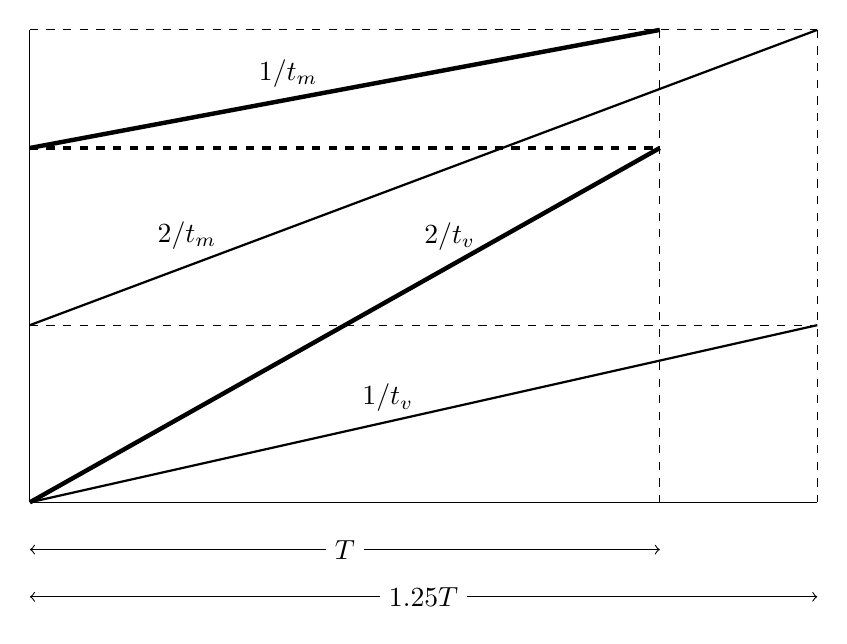
\begin{tikzpicture}
\draw (0,0) -- (10,0);
\draw (0,0) -- (0,6);
\draw[dashed] (0,6) -- (10,6);
\draw[ultra thick] (0,0) -- node[left,near end,xshift=-2mm] {$2/t_v$} (8,4.5)  coordinate (two-one);
\draw[ultra thick] (0,4.5)  -- node[left,xshift=-2mm,yshift=2mm] {$1/t_m$} (8,6) coordinate (two-one-finish);
\draw[dashed,ultra thick] (0,4.5) -- (8,4.5);
\draw[thick] (0,0) -- node[left,yshift=2mm] {$1/t_v$} (10,2.25)  coordinate (one-two);
\draw[thick] (0,2.25)  -- node[left,near start,yshift=2mm] {$2/t_m$} (10,6) coordinate (one-two-finish);
\draw[dashed] (0,2.25) -- (10,2.25);
\draw[dashed] (two-one-finish) -- (two-one-finish |- 0,0);
\draw[dashed] (one-two-finish) -- (one-two-finish |- 0,0);
\draw[<->] (0,-.6) -- node[fill=white] {$T$} (two-one-finish |- 0,-.6);
\draw[<->] (0,-1.2) -- node[fill=white] {$1.25 T$} (one-two-finish |- 0,-1.2);
\end{tikzpicture}
\end{center}


נסמן את הזמנים לצביעת כל הדלתות. 
$=t_v$
הזמן שלוקח צבע ותיק,
$=t_m$
הזמן שלוקח צבע מתלמד,
$=T$
הזמן שלוקח שני צבעים ותיקים וצבע מתלמד אחד.

\smallskip

\noindent\textbf{הסבר על התרשים:}
אמנם הצבעים עובדים במקביל אבל מבחינת התרשים הם
\textbf{מחלקים}
את עבודה )הציר האנכי(. לכן בתרשים מסומן כאילו שצבע )או זוג צבעים( מסיים את חלקו בעבודה ואחר כך הצבע )או הזוג( השני מתחיל את חלקו. מה שחשוב לראות הוא ששני החלקים מסתכמים ליחידת העבודה המליאה. השתמשתי בקווים בעובי שונה ובצבע שונה כדי לבדל את שני ההרכבים: שני ותיקים ומתלמד לעומת ותיק ושני מתלמדים.

ההספקים מתקבלים מעבודה חלקי זמן ורשומים כשיפועים על התרשים.  אפשר להתייחס לזוג צבעים כצבע אחד עם הספק כפול.

\smallskip

מהתרשים רואים ששני ההרכבים סיימו את העבודה ומכאן המשוואה:
\[
\frac{2}{t_v}T + \frac{1}{t_m} T = \frac{1}{t_v} \cdot 1.25T + \frac{2}{t_m} \cdot 1.25 T\,.
\]
נחלק ב-
$T$
)שבעצם מיותר כי כל יחידת זמן, אפילו
$1$,
מתאימה(, נכפיל ב-
$t_m$,
ונקבל:
\[
\frac{t_m}{t_v}=2\,.
\]

\paragraph{סעיף ב}

\begin{center}
\selectlanguage{english}
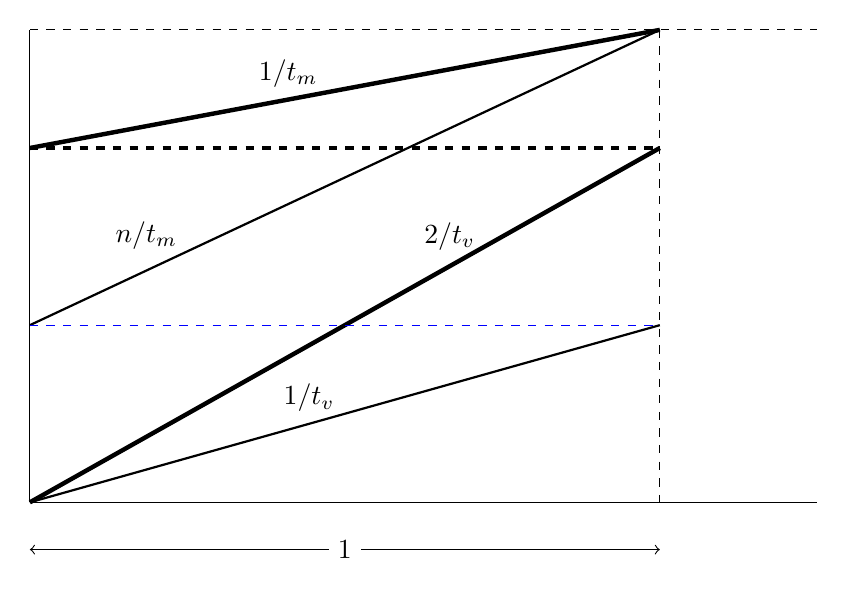
\begin{tikzpicture}
\draw (0,0) -- (10,0);
\draw (0,0) -- (0,6);
\draw[dashed] (0,6) -- (10,6);
\draw[ultra thick] (0,0) -- node[left,near end,xshift=-2mm] {$2/t_v$} (8,4.5)  coordinate (two-one);
\draw[ultra thick] (0,4.5)  -- node[left,xshift=-2mm,yshift=2mm] {$1/t_m$} (8,6) coordinate (two-one-finish);
\draw[dashed,ultra thick] (0,4.5) -- (8,4.5);
\draw[thick] (0,0) -- node[left,yshift=2mm] {$1/t_v$} (8,2.25)  coordinate (one-two);
\draw[thick] (0,2.25)  -- node[left,near start,yshift=2mm] {$n/t_m$} (8,6) coordinate (one-two-finish);
\draw[dashed,blue] (0,2.25) -- (8,2.25);
\draw[dashed] (two-one-finish) -- (two-one-finish |- 0,0);
\draw[<->] (0,-.6) -- node[fill=white] {$1$} (two-one-finish |- 0,-.6);
\end{tikzpicture}
\end{center}

הפעם נשתמש ב-
$1$
כיחידת זמן. העבודה של שני ההרכבים שווה ולכן:
\[
\frac{2}{t_v} + \frac{1}{t_m} = \frac{1}{t_v} + \frac{n}{t_m}\,.
\]
נכפיל ב-
$t_m$,
נשתמש ביחס שחישבנו בסעיף א' ונקבל:
\[
2=\frac{t_m}{t_v}=n-1\,,
\]
והתשובה היא
$n=3$.

\newpage
%%%%%%%%%%%%%%%%%%%%%%%%%%%%%%%%%%%%%%%%%%%%%%%%%%%%%%%%%%%%%%%%

\section*{קיץ תשע"ו, מועד ב'}

\begin{center}
\selectlanguage{english}
\includegraphics[width=\textwidth]{summer-2016b-1}
\end{center}

\paragraph{סעיף א}

\begin{center}
\selectlanguage{english}
\begin{tikzpicture}
\draw (0,0) -- (10,0);
\draw (0,0) -- (0,6);
\draw[dashed] (0,6) -- (10,6);
\draw[thick,name path=gal] (0,0) -- node[right,near end,xshift=3mm] {
\R{גל}
} node[right,xshift=7mm] {$\displaystyle\frac{1}{7}$}(10,6);
\draw[thick,name path=danny] (1.2,0) -- node[left,near end,xshift=-3mm] {
\R{דני}
} node[left,yshift=3mm] {$\displaystyle\frac{1}{(1-t)+4}$} (7,6);
\draw[dashed] (7,6) -- (7,0);
\draw[dashed] (10,6) -- (10,0);
\path [name intersections={of=gal and danny,by=inter}];
\fill (inter) circle [radius=2pt];
\draw[dashed] (inter) -- (inter |- 0,0);
\draw[dashed] (inter) -- (inter -| 0,0);
\node[below] at (0,0) {\p{0800}};
\node[below] at (1.2,0) {$t$};
\node[below] at (inter |- 0,0) {\p{0900}};
\node[below] at (7,0) {\p{1300}};
\node[below] at (10,0) {\p{1500}};
\end{tikzpicture}
\end{center}

נסמן:
$=t$
הזמן שדני התחיל בהרכבה.

\smallskip

ההספקים הרשומים על התרשים מתקבלים מהנתונים על הזמן להשלמת ההרכבה.

\smallskip

נתון שבשעה 
\L{\p{0900}}
שניהם סיימו להרכיב אותו כמות של מחשבים:
\[
\frac{1}{7}\cdot 1 = \frac{1}{5-t} \cdot (1-t)\,.
\]
מתקבל שדני התחיל לעבוד
$\displaystyle\frac{1}{3}$
שעה לאחר
\L{\p{0800}}.

\paragraph{סעיף ב}

\begin{center}
\selectlanguage{english}
\begin{tikzpicture}
\draw (0,0) -- (10,0);
\draw (0,0) -- (0,6);
\draw[dashed] (0,6) -- (10,6);
\draw[thick] (0,0) -- node[right,near end,xshift=2mm,yshift=-2mm] {
\R{גל}
} node[right,xshift=6mm,yshift=-3mm] {$\displaystyle\frac{1}{7}$}(8,2.5);
\draw[thick] (0,0) -- node[left,near end,xshift=-3mm] {
\R{דני}
} node[left,xshift=-2mm,yshift=3mm] {$\displaystyle\frac{3}{14}$} (8,6);
\draw[dashed] (8,6) -- (8,0);
\draw[<->] (0,-.6) -- node[fill=white] {$T$} (8,-.6);
\draw[<->] (8.6,0) -- node[fill=white] {$w_g$} (8.6,2.5);
\draw[<->] (9.2,0) -- node[fill=white] {$w_d$} (9.2,6);
\end{tikzpicture}
\end{center}
נסמן: 
$=T$
הזמן ששניהם עבדו ביום השני. על התרשים סימנו גם את כמות העבודה שעשה כל אחד מהם:
$=w_g$
העבודה של גל,
$=w_d$
העבודה של דני.

\smallskip

מסעיף א' אנו יודעים מתי דני התחיל לעבוד ביום הראשון וניתן לחשב שההספק שלו:
\[
\frac{1}{\left(1-\frac{1}{3}\right)+4}=\frac{3}{14}\,.
\]

\smallskip

נתון שהם סיימו אותה כמות עבודה כמו היום הראשון כאשר כל אחד סיים יחידה שלמה של עבודה. מתקבלת המשוואה:
\[
1+1=w_g+w_d=\frac{1}{7}T + \frac{3}{14}T\,,
\]
והפתרון הוא 
$T=\displaystyle \frac{28}{5}$.

\newpage

%%%%%%%%%%%%%%%%%%%%%%%%%%%%%%%%%%%%%%%%%%%%%%%%%%%%%%%%%%%%%%%%

\section*{חורף תשע"ז}

\begin{center}
\selectlanguage{english}
\includegraphics[width=.9\textwidth]{winter-2017-1}
\end{center}

\paragraph{סעיף א}

\begin{center}
\selectlanguage{english}
\begin{tikzpicture}[scale=.8]
\draw (0,0) -- (10,0);
\draw (0,0) -- (0,6);
\draw[dashed] (0,6) -- (10,6);
\draw[thick] (0,0) -- node[right,near end,xshift=2mm,yshift=-2mm] {
\R{ב}
} node[right,xshift=12mm,yshift=4mm] {$\displaystyle\frac{1}{2m}$}(9,6);
\draw[thick] (0,0) -- node[left,near end,xshift=-3mm] {
\R{א}
} node[left,xshift=-2mm,yshift=3mm] {$\displaystyle\frac{1}{m}$} (4.5,6);
\draw[dashed] (9,6) -- (9,0);
\draw[dashed] (4.5,6) -- (4.5,0);
\draw[<->] (0,-.6) -- node[fill=white] {$m$} (4.5,-.6);
\draw[<->] (0,-1.2) -- node[fill=white] {$2m$} (9,-1.2);
\end{tikzpicture}
\end{center}
כאשר שני הצינורות פתוחים, ההספק הכולל הוא סכום ההספקים של הצינורות. לפי הנתונים:
\[
1/\left(\frac{1}{m}+\frac{1}{2m}\right) > 4\,,
\]
כך ש-
$m>6$.

\begin{center}
\selectlanguage{english}
\begin{tikzpicture}
\draw (0,0) -- (10,0);
\draw (0,0) -- (0,5);
%\draw[dashed] (0,6) -- (10,6);
\draw[thick] (4,0) -- node[above,near end,yshift=2mm] {
\R{ב}
} node[above,near start,yshift=2mm] {$\displaystyle\frac{1}{2m}$}(8,1);
\draw[thick] (0,0) -- node[left,near end,xshift=-3mm] {
\R{א}
} node[left,xshift=-2mm,yshift=3mm] {$\displaystyle\frac{1}{m}$} (8,4);
\draw[dashed] (8,4) -- (8,0);
\draw[dashed] (4,2) -- (4,0);
\draw[<->] (0,-.6) -- node[fill=white] {$2$} (4,-.6);
\draw[<->] (0,-1.2) -- node[fill=white] {$4$} (8,-1.2);
\draw[<->] (9,0) -- node[fill=white] {$w_a$} (9,4);
\draw[<->] (8.5,0) -- node[fill=white] {$w_b$} (8.5,1);
\end{tikzpicture}
\end{center}
נסמן:
$=w_a$
כמות המים שמילא צינור א',
$=w_b$
כמות המים שמילא צינור ב'.

\smallskip

כמות המים בבריכה לאחר ארבע שעות שווה לסכום הכמויות שכל צינור מילא והיא לפחות מחצית הבריכה:
\[
w_a + w_b = \frac{1}{m}\cdot 4 + \frac{1}{2m}\cdot 2 > \frac{1}{2}\,.
\]
מכאן,
$m<10$.

\paragraph{סעיף ב}

\begin{center}
\selectlanguage{english}
\begin{tikzpicture}[scale=.9]
\draw (0,0) -- (10,0);
\draw (0,0) -- (0,6);
\draw[dashed] (0,6) -- (10,6);
\draw[thick] (0,3) -- node[below right,xshift=10mm,yshift=-4mm] {$\displaystyle\frac{1}{m}-\frac{1}{2m}=\frac{1}{2m}$} (2,3.5);
\draw[->] (2.2,2.15) -- +(140:1.6cm);
\draw[thick] (2,3.5) -- node[left,xshift=-4mm,yshift=3mm] {$\displaystyle\frac{1}{m}+\frac{1}{2m}=\frac{3}{2m}$} (7,6);
\draw[dashed] (2,3.5) -- (2,0);
\draw[dashed] (2,3.5) -- (0,3.5);
\draw[dashed] (7,6) -- (7,0);
\draw[<->] (0,-.6) -- node[fill=white] {$1$} (2,-.6);
\draw[<->] (2,-1.2) -- node[fill=white] {$2.5$} (7,-1.2);
\node at (-.4,3) {$\displaystyle\frac{1}{2}$};
\end{tikzpicture}
\end{center}
כדי למלא את הבריכה, מתחילים ממחצית הכמות, מוסיפים )מחסירים כי שלילי( את הכמות של השעה הראשונה, ומוסיפים את הכמות מהתקופה השניה של שעתיים וחצי:
\[
\frac{1}{2} + \frac{1}{2m}\cdot 1 + \frac{3}{2m}\cdot 2.5 = 1\,.
\]
הפתרון הוא
$m=8.5$.

%%%%%%%%%%%%%%%%%%%%%%%%%%%%%%%%%%%%%%%%%%%%%%%%%%%%%%%%%%%%%%%%

\newpage

\section*{חורף תשע"ח}

\begin{center}
\selectlanguage{english}
\includegraphics[width=1.1\textwidth]{winter-2018-1}
\end{center}

\begin{center}
\selectlanguage{english}
\begin{tikzpicture}[scale=1.25]
\draw (0,0) -- (10,0);
\draw (0,0) -- (0,6);
\node at (-.5,1) {$\frac{1}{6}V_1$};
\node at (-.5,3) {$\frac{1}{2}V_1$};
\node at (-.5,6) {$V_1$};

\fill (0,0) circle [radius=2pt];
\draw[dashed] (0,1) -- (1,1);
\draw (0,0) -- node[below,xshift=4pt] {$4x$} (1,1);
\fill (1,1) circle [radius=2pt];

\draw[dashed] (0,3) -- (4,3);
\draw (1,1) -- node[below,xshift=4pt] {$3x$} (4,3);
\fill (4,3) circle [radius=2pt];

\draw[dashed] (0,6) -- (10,6);
\draw (4,3) -- node[below,xshift=4pt] {$x$} (10,6);
\fill (10,6) circle [radius=2pt];

\draw[dashed] (1,1) -- (1,0);
\draw[dashed] (4,3) -- (4,0);
\draw[dashed] (10,6) -- (10,0);

\draw[<->] (10.5,0) -- node[fill=white] {$V_2$} (10.5,5.5);

\fill (1,0) circle [radius=2pt];
\draw (1,0) -- node[below,xshift=4pt] {$x$} (4,1);
\fill (4,1) circle [radius=2pt];
\draw (4,1) -- node[below,xshift=4pt] {$3x$} (10,5.5);
\fill (10,5.5) circle [radius=2pt];

\draw[<->] (0,-.5) -- node[fill=white] {$t_1$} (1,-.5);
\draw[<->] (1,-.5) -- node[fill=white] {$t_2$} (4,-.5);
\draw[<->] (4,-.5) -- node[fill=white] {$t_3$} (10,-.5);


\end{tikzpicture}
\end{center}


נסמן:
$=x$
קצב המילוי של כל צינור בנפרד. 
$=t_1, t_2, t_3$
פרקי הזמן לכל חלוקה של הצינורות בין הבריכות. הקו העליון בתרשים מתאר את המילוי של בריכה א', והקו התחתון מתאר את מילוי של בריכה ב'.

נכתוב את המשוואות ההספק עבור בריכה א':
\[
4x t_1 = \frac{1}{6}V_1,\quad 3x t_2 = (\frac{1}{2}-\frac{1}{6})V_1,\quad xt_3=(1-\frac{1}{2})V_1\,,
\]
ונשתמש בהן כדי לחשב את פרקי הזמן כתלות בנפח בבריכה:
\[
t_1 = \frac{V_1}{24x},\quad t_2 = \frac{V_1}{9x},\quad t_3=\frac{V_1}{2x}\,.
\]
מהתרשים אנו רואים שאפשר לבטא את הנפח של
$V_2$
כסכום של שני חלקים נפרדים: הראשון בפרק הזמן
$t_2$
והשני בפרק הזמן
$t_3$.
כאשר נציב את המשוואות שקבלנו עבור בפרקי הזמן, נקבל את הנפח של
$V_2$
כתלות ב-%
$V_1$
בלבד, כי המשתנה 
$x$ מצטמצם:
\[
V_2 = xt_2 + 3xt_3 = \frac{x V_1}{9x} + \frac{3x V_1}{2x}\ = \frac{29}{18}V_1\,.
\]
מכאן קבלנו את התשובה הדרושה, היחס בין שני הנפחים:
\[
\frac{V_1}{V_2} = \frac{18}{29}\,.
\]
\begin{itemize}
\item 
לא היה צורך במידע על ההספק בפרק הזמן הראשון כאשר רק בריכה א' מתמלאת.
\item
מהתשובה אנו רואים שהנפח של בריכה ב' גדול מהנפח של בריכה א'. לא ידענו זאת לפני שפתרנו את השאלה, והתרשים מראה את המצב ההפוך. אין לזה חשיבות. מטרת התרשים היא להציג את התסריט כדי שנוכל לכתוב את המשוואות הנכונות. כאן, חשוב לשים לב שפרק הזמן הראשון לא נחוץ לפתרון, ושהמילוי של בריכה ב' מתבצע בשני שלבים שזמנם זהים לזמנם של שלבי המילוי של בריכה א'.

\end{itemize}

\end{document}


\tikzsetfigurename{series}
% !TeX root = chapter-1-2-3.tex

\selectlanguage{hebrew}

\chapter{סדרות}


%%%%%%%%%%%%%%%%%%%%%%%%%%%%%%%%%%%%%%%%%%%%%%%%%%%%%%%%%%%%%%%%%%%

\section{קיץ תשע"ח מועד ב}

\begin{center}
\selectlanguage{english}
\includegraphics[width=\textwidth]{summer-2018b-2}
\end{center}
\vspace{-1ex}

\textbf{סעיף א}

נציב את כלל הנסיגה בתוך עצמו:
\[
a_{n+1} = -\frac{c^{n-2}}{a_n} = -\frac{c^{n-2}}{\displaystyle -\frac{c^{n-3}}{a_{n-1}}} = ca_{n-1}\,.
\]
המנה
$a_{n+1}/a_{n-1}=c$
קבועה לא תלוי בזוגיות של האיברים.

\textbf{סעיף ב}
$(1)$

הסדרות של הזוגיים והאי-זוגיים הן סדרות הנדסיות
\textbf{נפרדות},
ולכן יש לחשב את האיברים
$(a_1,a_3,a_5,a_7), (a_2,a_4,a_6)$
בנפרד:
\[
\renewcommand{\arraystretch}{2}
\begin{array}{l}
a_1=-\displaystyle\frac{1}{c},\;\;a_3=ca_1=-1,\;\;a_5=ca_3=-c,\;\;a_7=ca_5=-c^2\\
a_2=\displaystyle
-\frac{c^{1-2}}{a_1}=
-\frac{c^{-1}}{-\frac{1}{c}}=1,\;\;a_4=ca_2=c,\;\;a_6=ca_4=c^2\,.
\end{array}
\]
\textbf{סעיף ב}
$(2)$

כאשר מסכמים את האיברים הם מצטמצמים פרט לאיבר הראשון, ולכן
$S_7=-\frac{1}{c}$.

\newpage

\textbf{סעיף ב}
$(3)$

יש 
$n$ 
אי-זוגיים ו-%
$n-1$
זוגיים, ראו את הפתרון לבחינה של קיץ תשע"ו ב:
\[
S_{\mathit{odd}}+S_{\mathit{even}}=-\frac{1}{c}\frac{c^n-1}{c-1}+ 1\cdot\frac{c^{n-1}-1}{c-1}= \frac{-c^{n-1}+c^{-1} + c^{n-1}-1}{c-1}= -\frac{1}{c}\,.
\]
\textbf{סעיף ג}
$(1)$
\[
\frac{b_{n+1}}{b_n} = \frac{\displaystyle\frac{2}{a_{n+1}a_{n+2}}}{\displaystyle\frac{2}{a_{n}a_{n+1}}}= \frac{a_n}{a_{n+2}} =  \frac{1}{\displaystyle\frac{a_{n+2}}{a_n}} = \frac{1}{c}\,.
\]
\textbf{סעיף ג}
$(2)$

סדרה יורדת אם
$0<q=\displaystyle\frac{1}{c} < 1$.
נתון
$c>0$,
ולכן הסדרה יורדת אם
$c>1$.

\textbf{סעיף ג}
$(3)$

נתון שהסדרה היא הנדסית אינסופית יורדת. ניתן להשתמש בנוסחה 
$S=\displaystyle\frac{a_1q}{1-q}$:
\[
b_1=\frac{-2}{a_1a_2}= \frac{-2}{\displaystyle-\frac{1}{c}\cdot 1}=2c\,,\quad\quad
S_b = 2c\cdot\frac{1}{1-\displaystyle\frac{1}{c}}=\frac{2c^2}{c-1}\,.
\]


%%%%%%%%%%%%%%%%%%%%%%%%%%%%%%%%%%%%%%%%%%%%%%%%%%%%%%%%%%%%%%%%%%%
\np
\section{קיץ תשע"ח מועד א}

\begin{center}
\selectlanguage{english}
\includegraphics[width=.95\textwidth]{summer-2018a-2}
\end{center}

\textbf{סעיף א}

השאלה יפה כי היא דורשת חשיבה, לא חישובים! נבדוק את הטענות על סדרה מוכרת:
\[
1+ \frac{1}{2} + \frac{1}{4} + \frac{1}{8} + \cdots = 2\,.
\]
אם נהפוך את כל הסימנים למינוס, נקבל סדרה שסכומה שלילי:
\[
-1 - \frac{1}{2} - \frac{1}{4} - \frac{1}{8} - \cdots = -\left(1+ \frac{1}{2} + \frac{1}{4} + \frac{1}{8} + \cdots\right) = -2\,.
\]
ברור שהמנה עדיין חיובית
$\frac{1}{2}$.
לכן אפשר לפסול מייד תשובות 
\L{I, II, IV}
ונשאר רק תשובה
\L{III}.
סדרה הנדסית מתכנסת רק אם
$|q|<1$.
נבדוק: מהנוסחה עבור הסכום:
\[
S = \frac{a_1}{1-q}
\]
ניתן לראות שהסכום שלילי רק אם 
$a_1$
שלילי כי המכנה חיובי
$0 < 1-q < 2$.

\textbf{סעיף ב}

המנה של כל אחת מהסדרות היא
$q^2$
ולכן הסכומים הם:
\[
T = \frac{a_1}{1-q^2},\quad\quad R = \frac{a_1q}{1-q^2}\,.
\]
מהמשוואה הנתונה
$T+pR=0$,
נקבל
$\quad 1+pq=0\quad$
ו-%
$p=-\displaystyle\frac{1}{q}\quad$.

\textbf{סעיף ג}

הסדרה לא מתכנסת כי 
$|q|<1$
גורר
$|p|>1$.

\textbf{סעיף ד}

השאלה שואלת על
\textbf{הסדרה המקורית}
$a_n$
ולא על 
$b_n$.
נתון ש-%
$p$
שלילי ולכן
$q=-\displaystyle\frac{1}{p}$
חיובי. נתון שהסדרה מתכנסת ולכן
$0<q<1$.
מצאנו בסעיף א ש-%
$a_1$
שלילי ולכן
$a_{n+1}>a_n$.
נבדוק בדוגמה: אם 
$a_n=-6,q=\frac{1}{2}$,
אז:
\[
a_{n+1} = a_nq = -6\cdot \frac{1}{2} = -3 \;> \; -6 =a_n\,.
\]


%%%%%%%%%%%%%%%%%%%%%%%%%%%%%%%%%%%%%%%%%%%%%%%%%%%%%%%%%%%%%%%%%%%

\np
\section{חורף תשע"ח}

\begin{center}
\selectlanguage{english}
\includegraphics[width=.95\textwidth]{winter-2018-2}
\end{center}

\vspace{-3ex}

\textbf{סעיף א}

נציב 
$a_1+(n-1)d$
עבור 
$a_7,a_{17}$
ונשתמש במשוואה הנתונה
$a_7=-a_{17}$.
\begin{eqnarray*}
a_1+6d &=& -(a_1+16d)\\
a_1+11d &=& 0\\
a_{12} &=&a_1+11d = 0
\end{eqnarray*}
\textbf{סעיף ב}
$(1)$

נשווה את
$-a_1$
לנוסחה לאיבר כללי:
\[
-a_1 = a_n = a_1 + (n-1)d\,.
\]
נציב
$a_1=-11d$:
\[
-(-11d) = -11d + (n-1)d\,.
\]
$d$
מצטמצם ונקבל
$n=23$.

\textbf{סעיף ב}
$(2)$

נציב
$a_1=-11d$
 בנוסחה לסכום של סדרה חשבונית:
\[
\frac{n}{2}(2a_1+(n-1)d) = \frac{n}{2}(2\cdot -11d+(n-1)d) =\frac{dn}{2} (n-23)=0\,.
\]
%\begin{eqnarray*}
%0 &=& \frac{n}{2}(2a_1+(n-1)d)\\
%&=& \frac{n}{2}(2\cdot -11d+(n-1)d)\\
%&=& \frac{dn}{2} (n-23)\,.
%\end{eqnarray*}
נתון שההפרש 
$d$
שונה מאפס וש-%
$n$
מספר טבעי ולכן חיובי, כך שהביטוי מתאפס רק עבור
$n=23$.

\textbf{סעיף ג}

אם איבר חיובי וההפרש חיובי, המכפלה של שני איברים עוקבים היא חיובית, וכך גם אם שניהם שליליים. האפשרות היחידה לקבל מכפלה שלילית היא איבר חיובי והפרש שלילי או להיפך:
\[
\begin{array}{l}
a_k<0,\; a_{k+1}>0\\
a_k>0,\; a_{k+1}<0\,.
\end{array}
\]
אבל ידוע שאחד האיברים בסדרה 
$(a_{12})$
הוא אפס:
\[
\begin{array}{l}
a_k<0,\; a_{k+1}=0,\; a_{k+2}>0\\
a_k>0,\; a_{k+1}=0,\; a_{k+2}<0\,,
\end{array}
\]
ולכן המכפלה של זוג איברים עוקבים חייבת להיות חיובית או אפס.

\textbf{סעיף ד}
נרשום את הסדרה:
\[
a_1,\; a_2,\; \ldots,\; a_{11},\; 0,\; -a_{11},\; \ldots,\; -a_2,\; -a_1,\; \ldots\,.
\]
או ש-%
$11$
האיברים הראשונים שליליים אם ההפרש חיובי, או כל האיברים לאחר האיבר
$a_{12}=0$
שליליים אם ההפרש שלילי.



%%%%%%%%%%%%%%%%%%%%%%%%%%%%%%%%%%%%%%%%%%%%%%%%%%%%%%%%%%%%%%%%%%%
\np
\section{קיץ תשע"ז מועד ב}

\begin{center}
\selectlanguage{english}
\includegraphics[width=.95\textwidth]{summer-2017b-2}
\end{center}

שאלה זו שונה משאלות אחרות כי נתון ביטוי עבור
\textbf{הסכומים}
ולא עבור האיברים בסדרה.

\textbf{סעיף א}

ניתן לחשב:
\[
a_1=S_1=k-\frac{1}{9}\,, \quad\quad\quad a_n=S_{n}-S_{n-1}=\left(k-\frac{1}{3^{n+1}}\right)-\left(k-\frac{1}{3^{n}}\right)=\frac{2}{3^{n+1}}\,.
\]

\textbf{סעיף ב}

המנה
$q=\displaystyle\frac{a_{n+1}}{a_{n}}=\frac{1}{3}$
לא תלויה ב-%
$k$.
במבט ראשון נראה שהתשובה היא שהסדרה היא הנדסית עבור כל ערך של
$k$,
אולם זו
\textbf{טעות}.
המנה המתקבלת מ-%
$\displaystyle\frac{a_2}{a_1}$
חייבת להיות
\textbf{שווה}
למנה המתקבלת במקרה הכללי
$\displaystyle\frac{a_{n+1}}{a_{n}}$.
נחשב:
\[
\frac{a_2}{a_1}=\frac{\displaystyle\frac{2}{3^3}}{\displaystyle k-\frac{1}{9}} = \frac{a_{n+1}}{a_n}=\frac{1}{3}\,.
\]
הפתרון היחיד הוא
$k=\frac{1}{3}$
ואז האיבר הראשון הוא
$\frac{1}{3}-\frac{1}{9}=\frac{2}{9}$.

\textbf{סעיף ג}

הסדרה החדשה הנדסית כי הסדרה המקורית הנדסית, והמנה של הסדרה החדשה היא המנה המקורית לחזקת
$3\cdot 2=6$:
נבחרו כל איבר שלישי מהסדרה המקורית וכל איבר הוא הריבוע של האיבר המקורי. האיבר הראשון של הסדרה החדשה היא האיבר השני של הסדרה המקורית לחזקת שניים. פתרון אחר הוא לחשב את המנה לפי הנוסחה:
\[
q'=\frac{a_{n+3}}{a_n}=\frac{\left(\frac{2}{3^{n+4}}\right)^2}     {\left(\frac{2}{3^{n+1}}\right)^2}=\left(\frac{1}{3^3}\right)^2=\frac{1}{729}\,.
\]
האיבר הראשון הוא
\[
a'_1 = a_2^2=\left(a_1q\right)^2=\left(\frac{2}{9}\cdot\frac{1}{3}\right)^2=\frac{4}{729}\,,
\]
והסכום הוא:
\[
S'=\frac{a'_1}{1-q'}=
\frac{\displaystyle\frac{4}{729}}{1-\displaystyle\frac{1}{729}}= \frac{1}{182}\,.
\]

%%%%%%%%%%%%%%%%%%%%%%%%%%%%%%%%%%%%%%%%%%%%%%%%%%%%%%%%%%%%%%%%%%%
\np
\section{קיץ תשע"ז מועד א}

\begin{center}
\selectlanguage{english}
\includegraphics[width=.95\textwidth]{summer-2017a-2}
\end{center}
הנוסחה ל-%
$a_n$
אינה כלל נסיגה כי איברים של הסדרה לא מופיעים בצד הימני של המשוואה. המשוואה מגדריה את
$a_n$
כפונקציה של
$n$.
נתון שהסדרות 
$b_n,c_n$
הנדסיות או לא נתון שום אפיון של הסדרה המקורית
$a_n$.
נחשב ערכים של הסדרה המקורית לפי הפונקציה:
\[
a_3=\frac{(2^3+1)(2^3-1)}{2^3}=\frac{63}{8}\,, \quad\quad a_6=\frac{(2^6+1)(2^6-1)}{2^6}= \frac{65\cdot 63}{64}\,.
\]
\textbf{סעיף א} 
$(1,2)$

ההגדרה
$a_n=b_n-c_n$
מאפשרת לחשב את הערכים:
\[
b_3=a_3+c_3=\frac{63}{8}+\frac{1}{8}=8\,,\quad\quad c_6=b_6-a_6=64-\frac{65\cdot 63}{64}=\frac{1}{64}\,.
\]
אי אפשר לחשב את מנות של
$b_n,c_n$,
על ידי חילוק של איברים סמוכים כי אין לנו אותם. במקום זה, ננצל את העבודה שנתון שהסדרות הנדסיות כדי לחשב את המנות והאיברים הראשוניים:

\[
\begin{array}{|@{\hspace{2em}}c@{\hspace{2em}}|c|@{\hspace{2em}}c@{\hspace{2em}}|c|}
\hline
\rule[-1.5ex]{0pt}{4ex}b_6&q_b&b_3&b_1\\\hline
\rule[-3.5ex]{0pt}{9ex}b_3q_b^3 & \displaystyle\sqrt[3]{\frac{b_6}{b_3}}=\sqrt[3]{8}=2&
b_1 q_b^2 & \displaystyle\frac{b_3}{q_b^2}=\frac{8}{4}=2\\\hline\hline
\rule[-1.5ex]{0pt}{4ex}c_6&q_c&c_3&c_1\\\hline
c_3q_c^3 & \displaystyle\sqrt[3]{\frac{c_6}{c_3}} =\sqrt[3]{\frac{1}{8}} = \frac{1}{2}&
\rule[-3.5ex]{0pt}{9ex}c_1 q_c^2 & \displaystyle\frac{c_3}{q_c^2}=\frac{1/8}{1/4}=\frac{1}{2}\\
\hline
\end{array}
\]

\textbf{סעיף ב}

נוכיח תוך שימוש בחוקים של חיבור של מספרים שלמים:
\begin{eqnarray*}
C_n &=& (b_1-a_1) + (b_2 - a_2) + \cdots + (b_n-a_n)\\
&=&(b_1 + b_2 + \cdots + b_n) - (a_1 + a_2 + \cdots + a_n)\\
&=& B_n - A_n\,.
\end{eqnarray*}
\textbf{סעיף ג}

הוכחנו ש-%
$C_n=B_n-A_n$,
ונתונה שהסדרה 
$c_n$
הנדסית. חישבנו 
$q_c=\frac{1}{2},\,c_1=\frac{1}{2}$,
ולכן:
\[
C_n = \frac{1}{2}\cdot\frac{\displaystyle\left(\frac{1}{2}^n-1\right)}{\displaystyle\left(\frac{1}{2}-1\right)}=1-2^{-n}\,.
\]
בדיקה מראה ש-%
$0.9 \not< 1-2^{-3}=0.875$,
אבל
$0.9 < 1-2^{-4}=0.9375 < 1$.

השאלה מבקשת את
\textbf{כל הערכים}
של
$n$
המקיימים את האי-שוויון, ולכן התשובה המליאה היא 
\textbf{כל מספר גדול או שווה ל-}%
$4$,
כי גם עבור מספרים גדולים מ-%
$4$
הביטוי
$1-2^{-n}$
מקיים את האי-שוויון.

%%%%%%%%%%%%%%%%%%%%%%%%%%%%%%%%%%%%%%%%%%%%%%%%%%%%%%%%%%%%%%%%%%%
\np
\section{חורף תשע"ז}

\begin{center}
\selectlanguage{english}
\includegraphics[width=.95\textwidth]{winter-2017-2}
\end{center}

\vspace{-2ex}

\textbf{סעיף א}

נחשב את המנה על ידי הצבה עבור 
$b_n$
לפי ההגדרה, ואחר כך הצבה עבור 
$a_{n+1}$
לפי כלל הנסיגה. נקבל מנה קבועה ולכן הסדרה הנדסית:
\[
\frac{b_{n+1}}{b_n} = \frac{\displaystyle\frac{1}{a_{n+1}}+2}{\displaystyle\frac{1}{a_{n}}+2}= \frac{\displaystyle\frac{4a_n+3}{a_n}+2}{\displaystyle\frac{1}{a_{n}}+2}=\frac{3(2a_n+1)}{2a_n+1}=3\,.
\]
\vspace{-3ex}

\textbf{סעיף ב}

לא נתון שהסדרה $a_n$ הנדסית, אבל בסעיף א הוכחנו שהסדרה  
$b_n$
הנדסית, ולכן ניתן לבטא את סכום הסדרה
$\displaystyle\frac{1}{a_n}$
כסכום של הסדרה
$b_n$
על ידי ההצבה 
$\displaystyle\frac{1}{a_i} = b_i - 2$:
\[
\frac{1}{a_1} + \cdots + \frac{1}{a_n}=(b_1-2) + \cdots + (b_n-2)=b_1+\cdots+b_n- 2n\,.
\]
בסעיף א חישבנו 
$q_b=3$
ו-%
$b_1=\displaystyle\frac{1}{a_1}+2=\displaystyle\frac{1}{-1}+2=1$.
סכום הסדרה של ההפוכים של 
$a_n$
הוא:
\[
b_1+\cdots+b_n- 2n=\frac{1(3^n-1)}{3-1} - 2n = \frac{3^n - 4n -1}{2}\,.
\]
\textbf{סעיף ג}

לפי ההגדרה של 
$b_n$
נוכל לבטא את הסכום כך:
\[
(b_1 - 2) - (b_2 - 2) + \cdots + (b_{n-1} - 2) + (b_n - 2)\,.
\]
נתון שמספר האיברים זוגי ולכן סכום הקבועים מתאפס. הסכום של איברי
$b_i$
הוא:
\[
b_1-b_2+\cdots+b_{n-1}-b_n=\frac{1((-3)^n-1)}{-3-1}=\frac{3^n-1}{-4}\,.
\]
נתון שמספר האיברים זוגי ולכן סימני השלילה ב-%
$(-3)^n$
מצטמצמים.


%%%%%%%%%%%%%%%%%%%%%%%%%%%%%%%%%%%%%%%%%%%%%%%%%%%%%%%%%%%%%%%%%%%

\np
\section{קיץ תשע"ו מועד ב}

\begin{center}
\selectlanguage{english}
\includegraphics[width=.95\textwidth]{summer-2016b-2}
\end{center}
\vspace{-1ex}

\textbf{סעיף א}
$(1)$

מספר האיברים החדשים הוא
$n-1$,
כפי שרואים אם רושמים את הסדרה:
\[
a_1,\; a'_1,\; a_2,\; a'_2,\; \ldots,\; a_{n-1},\; a'_{n-1},\; a_n\,.
\]
נתון שהסדרה החדשה גם היא חשבונית. הפרש הסדרה אינו מספר שלם אלא
$1.5$!
המנה של סכומי הסדרות היא:
\[
\frac{S_{\mathit{new}}}{S_{\mathit{old}}}= \frac{\displaystyle\frac{2n-1}{2}(2a_1+1.5(2n-1-1))}{\displaystyle\frac{n}{2}(2a_1+3(n-1))}=\frac{\displaystyle\frac{2n-1}{2}(2a_1+3(n-1))}{\displaystyle\frac{n}{2}(2a_1+3(n-1))}=\frac{2n-1}{n}\,.
\]
\textbf{סעיף א}
$(2)$

מ-%
$\displaystyle\frac{2n-1}{n}=1.9$
נקבל
$n=10$.

נתון שהסדרה החדשה חשבונית ולכן גם סדרת האיברים החדשים חשבונית:
\[
a'_{i+1}-a'_{i}=a'_{i+1}-(a_{i+1}-a_{i+1})-a'_i=(a'_{i+1}-a_{i+1})+(a_{i+1}-a'_i)=\frac{d}{2}+\frac{d}{2}=3\,.
\]
ניתן לבטא את האיבר הראשון כ-%
$a'_1=a_1+1.5$,
ולחשב את
$a_1$
מהנוסחה לסכום הנתון:
\[
\frac{10-1}{2}(2(a_1+1.5)+((10-1)-1)\cdot 3) = 130.5\,,\quad\quad 9a_1=9\,,\quad\quad a_1=1\,.
\]
\textbf{סעיף ב}

השאלה מכלילה את השאלה בסעיף א על ידי הכנסת
$k$
איברים חדשים בין כל שני איברים סמוכים של הסדרה המקורית. נתון גם שהסדרה החדשה
\textbf{חשבונית},
ולכן ההפרשים בין האיברים החדשים חייבים להיות שווים וסכומם שווה להפרש של הסדרה הנתונה שהוא
$3$.
\[
a_i,\; b_1,\; b_2,\; \ldots,\; b_k,\; a_{i+1}\,.
\]
יש
$k+1$
הפרשים שערכם
$\displaystyle\frac{3}{k+1}$.

%%%%%%%%%%%%%%%%%%%%%%%%%%%%%%%%%%%%%%%%%%%%%%%%%%%%%%%%%%%%%%%%%%%

\np
\section{קיץ תשע"ו מועד א}

\begin{center}
\selectlanguage{english}
\includegraphics[width=.95\textwidth]{summer-2016a-2}
\end{center}
\vspace{-2ex}

\textbf{סעיף א}

נציב
$a_n=a_1+(n-1)d$
עבור האיברים בסכום ונקבל משוואה אחת עם שני נעלמים:
\begin{eqnarray*}
(a_1+3d)+(a_1+7d)+(a_1+11d)+(a_1+15d)&=&224\\
a_1+9d&=&56\,.
\end{eqnarray*}
לא נתייאש וננסה לחשב את הסכום
$S_{19}$:
\[
S_{19}=\frac{19}{2}(2a_1+18d) = 19(a_1+9d)=19\cdot 56 = 1064\,.
\]
\textbf{סעיף ב}

נשווה את המשוואה הנתונה
$S_n=n\cdot a_n$
לנוסחה עבור סכום של סדרה חשבונית תוך הצבת הנוסחה לאיבר
$a_n$:
\begin{eqnarray*}
n\cdot a_n &=& \frac{n}{2}(2a_1+(n-1)d)\\
n(a_1+(n-1)d) &=&\frac{n}{2}(2a_1+(n-1)d)
\end{eqnarray*}
נפשט את המשוואה ונקבל 
$d=d/2$
שהפתרון היחיד שלה הוא
$d=0$.

\textbf{סעיף ג}

נציב
$0$
עבור 
$d$:
$a_1+9d=a_1+0=56$.

סעיף ד. במבט ראשון נראה שכדאי לצמצם את סכום הסדרה  ל-%
$b_{20}-b_1$,
אבל זה מבוי סתום כי אין לנו דרך לחשב את איברי הסדרה
$b_n$.
במקום זה נחשב את הביטויים
$(b_{i+1}-b_i)$:
\[
b_{i+1}-b_i=a_i+S_i=(a_1+(i-1)\cdot 0)+\frac{i}{2}(2a_1+(i-1)\cdot 0)=a_1(1+i)\,.
\]
הסכום הוא:
\[
a_1(2+3+\cdots+20)=56\cdot\frac{19}{2}(2\cdot 2 + (19-1)\cdot 1)=11704\,.
\]

%%%%%%%%%%%%%%%%%%%%%%%%%%%%%%%%%%%%%%%%%%%%%%%%%%%%%%%%%%%%%%%%%%%
\np
\section{חורף תשע"ו}

\begin{center}
\selectlanguage{english}
\includegraphics[width=.95\textwidth]{winter-2016-2}
\end{center}

\vspace{-3ex}

\textbf{סעיף א}

נתון:
\[
(1)\, a_4-a_3 = 4 (a_2-a_1),\quad (2)\, a_6 - a_1 = 31\,.
\]
נציב
$a_n=a_1q^{n-1}$ 
עבור
$a_2, a_3, a_4$,
ב-%
$(1)$,
ונקבל שלוש תשובות
$q=1,q=2,q=-2$.\\
נתון שהסדרה 
\textbf{עולה}
ולכן
$q=2$.
נציב 
$a_1q^5=32 a_1$
עבור
$a_6$
ב-%
$(2)$,
ונקבל
$a_1=1$.

\textbf{סעיף ב} 
$(1)$

עבור סדרה I:
\[
q_I=\frac{a_{n+1}\cdot a_{n+2}}{a_n\cdot a_{n+1}}=\frac{a_{n+2}}{a_n}=\frac{a_n\,q^2}{a_n}=q^2=4\,,
\]
והסדרה היא סדרה הנדסית עולה. עבור סדרה II:
\[
q_{II}=\left(\frac{a_{n+1}}{a_n} + \frac{a_{n+2}}{a_{n+1}}\right) / \left(\frac{a_{n}}{a_{n-1}} + \frac{a_{n+1}}{a_{n}}\right)=\frac{q+q}{q+q}=1\,.
\]
הסדרה הנדסית אבל
\textbf{לא עולה}.

\textbf{סעיף ב}
$(2)$

מסכום הסדרה ניתן לחשב את מספר האיברים בסדרה:
\begin{eqnarray*}
a_1\cdot a_2 + \cdots + a_{n+1} \cdot a_{n+2} &=& 2730\\
(1\cdot 2)\cdot \frac{4^{n+1}-1}{4-1}&=&2730\\
4^{n+1}&=&4096\\
n&=&5\,.
\end{eqnarray*}
\textbf{שימו לב!}
אמנם
$n=5$
אבל מספר האיברים בסדרה I הוא 
$n+1=6$:
\[
(1)\, a_1\cdot a_2,\;\; (2)\,a_2\cdot a_3,\;\;(3)\, a_3\cdot a_4,\;\; (4)\,a_4\cdot a_5,\;\; (5)\,a_5\cdot a_6,\;\; (6)\,a_6\cdot a_7 \;(= a_{n+1}\cdot a_{n+2})\,.
\]
\textbf{סעיף ב}
$(2)$

חישבנו
$q_{II}=1$.
נחשב את
$a_1^{II}$:
\[
a_1^{II}=\frac{a_{2}}{a_1} + \frac{a_{3}}{a_{2}}=\frac{2}{1}+\frac{4}{2}=4\,.
\]
\textbf{שימו לב!}
מספר האיברים בסדרה II הוא 
$5$:
\[
(1)\,\frac{a_2}{a_1}+\frac{a_3}{a_2},\;\;
(2)\,\frac{a_3}{a_2}+\frac{a_4}{a_3},\;\;
(3)\,\frac{a_4}{a_3}+\frac{a_5}{a_4},\;\;
(4)\,\frac{a_5}{a_4}+\frac{a_6}{a_5},\;\;
(5)\,\frac{a_6}{a_5}+\frac{a_7}{a_6} \left(= \frac{a_{n+1}}{a_n}+\frac{a_{n+2}}{a_{n+1}}\right)\,.
\]
ולכן סכום האיברים הוא:
\[
a_1^{II}+a_1^{II}\cdot 1 + a_1^{II}\cdot 1^2 + \cdots + a_1^{II}\cdot 1^4 = 4\cdot 5=20\,.
\]


%%%%%%%%%%%%%%%%%%%%%%%%%%%%%%%%%%%%%%%%%%%%%%%%%%%%%%%%%%%%%%%%%%%
\np

\section{קיץ תשע"ה, מועד ב}

\begin{center}
\selectlanguage{english}
\includegraphics[width=.95\textwidth]{summer-2015b-2}
\end{center}
\vspace{-2ex}

\textbf{סעיף א}

החילוק של איברים במרחק שני מקומות אחד מהשני לא תלוי בזוגיות:
\[
\frac{b_{n+2}}{b_n} = \frac{1}{2^{n+1}b_{n+1}}\cdot\frac{1}{b_n}=\frac{1}{2^{n+1}\cdot\displaystyle\frac{1}{2^nb_n}{b_n}}= \frac{1}{2}\,.
\]
\textbf{סעיף ב}

 נחשב בנפרד את הסכום של ארבעת האיברים הזוגיים וארבעת האיברים האי-זוגיים:
\begin{eqnarray*}
S_{\mathit{odd}} &=& b_1+b_3+b_5+b_7=b_1\left(1 + \frac{1}{2} + \frac{1}{4} +\frac{1}{8}\right)=\frac{15}{8}b_1\\
S_{\mathit{even}} &=& b_2+b_4+b_6+b_8=b_2\left(1 + \frac{1}{2} + \frac{1}{4} +\frac{1}{8}\right)=\frac{15}{8}b_2=\frac{15}{8}\cdot\frac{1}{2^1b_1}\,.
\end{eqnarray*}
מ:
\[
S_{\mathit{odd}} + S_{\mathit{even}} =\frac{15}{8}\left(b_1+\frac{1}{2b_1}\right)= 3\frac{7}{16}=\frac{55}{16}\,.
\]
נקבל משוואה ריבועית 
$6b_1^2-11b_1+3=0$
שיש לה שני פתרונות 
$b_1=\frac{3}{2},\,\frac{1}{3}$.


%%%%%%%%%%%%%%%%%%%%%%%%%%%%%%%%%%%%%%%%%%%%%%%%%%%%%%%%%%%%%%%%%%%
\np

\section{חורף תשע"ו}

\begin{center}
\selectlanguage{english}
\includegraphics[width=.95\textwidth]{winter-2016-2}
\end{center}

\textbf{סעיף א}

נתון:
\[
(1)\, a_4-a_3 = 4 (a_2-a_1),\quad (2)\, a_6 - a_1 = 31\,.
\]
נציב
$a_n=a_1q^{n-1}$ 
עבור
$a_2, a_3, a_4$,
ב-%
$(1)$,
ונקבל שלוש תשובות
$q=1,q=2,q=-2$.\\
נתון שהסדרה 
\textbf{עולה}
ולכן
$q=2$.
נציב 
$a_1q^5=32 a_1$
עבור
$a_6$
ב-%
$(2)$,
ונקבל
$a_1=1$.

\textbf{סעיף ב} 
$(1)$

עבור סדרה I:
\[
q_I=\frac{a_{n+1}\cdot a_{n+2}}{a_n\cdot a_{n+1}}=\frac{a_{n+2}}{a_n}=\frac{a_n\,q^2}{a_n}=q^2=4\,,
\]
והסדרה היא סדרה הנדסית עולה. עבור סדרה II:
\[
q_{II}=\left(\frac{a_{n+1}}{a_n} + \frac{a_{n+2}}{a_{n+1}}\right) / \left(\frac{a_{n}}{a_{n-1}} + \frac{a_{n+1}}{a_{n}}\right)=\frac{q+q}{q+q}=1\,.
\]
הסדרה הנדסית אבל
\textbf{לא עולה}.

\textbf{סעיף ב}
$(2)$

מסכום הסדרה ניתן לחשב את מספר האיברים בסדרה:
\begin{eqnarray*}
a_1\cdot a_2 + \cdots + a_{n+1} \cdot a_{n+2} &=& 2730\\
(1\cdot 2)\cdot \frac{4^{n+1}-1}{4-1}&=&2730\\
4^{n+1}&=&4096\\
n&=&5\,.
\end{eqnarray*}
\textbf{שימו לב!}
אמנם
$n=5$
אבל מספר האיברים בסדרה I הוא 
$n+1=6$:
\[
(1)\, a_1\cdot a_2,\;\; (2)\,a_2\cdot a_3,\;\;(3)\, a_3\cdot a_4,\;\; (4)\,a_4\cdot a_5,\;\; (5)\,a_5\cdot a_6,\;\; (6)\,a_6\cdot a_7 \;(= a_{n+1}\cdot a_{n+2})\,.
\]
\textbf{סעיף ב}
$(3)$

חישבנו
$q_{II}=1$.
נחשב את
$a_1^{II}$:
\[
a_1^{II}=\frac{a_{2}}{a_1} + \frac{a_{3}}{a_{2}}=\frac{2}{1}+\frac{4}{2}=4\,.
\]
\textbf{שימו לב!}
מספר האיברים בסדרה II הוא 
$5$:
\[
(1)\,\frac{a_2}{a_1}+\frac{a_3}{a_2},\;\;
(2)\,\frac{a_3}{a_2}+\frac{a_4}{a_3},\;\;
(3)\,\frac{a_4}{a_3}+\frac{a_5}{a_4},\;\;
(4)\,\frac{a_5}{a_4}+\frac{a_6}{a_5},\;\;
(5)\,\frac{a_6}{a_5}+\frac{a_7}{a_6} \left(= \frac{a_{n+1}}{a_n}+\frac{a_{n+2}}{a_{n+1}}\right)\,.
\]
ולכן סכום האיברים הוא:
\[
a_1^{II}+a_1^{II}\cdot 1 + a_1^{II}\cdot 1^2 + \cdots + a_1^{II}\cdot 1^4 = 4\cdot 5=20\,.
\]

%%%%%%%%%%%%%%%%%%%%%%%%%%%%%%%%%%%%%%%%%%%%%%%%%%%%%%%%%%%%%%%%%%%
\np
\section{קיץ תשע"ה מועד ב}

\begin{center}
\selectlanguage{english}
\includegraphics[width=.95\textwidth]{summer-2015b-2}
\end{center}
\vspace{-2ex}

\textbf{סעיף א}

החילוק של איברים במרחק שני מקומות אחד מהשני לא תלוי בזוגיות:
\[
\frac{b_{n+2}}{b_n} = \frac{1}{2^{n+1}b_{n+1}}\cdot\frac{1}{b_n}=\frac{1}{2^{n+1}\cdot\displaystyle\frac{1}{2^nb_n}{b_n}}= \frac{1}{2}\,.
\]
\textbf{סעיף ב}

נחשב בנפרד את הסכום של ארבעת האיברים הזוגיים וארבעת האיברים האי-זוגיים:
\begin{eqnarray*}
S_{\mathit{odd}} &=& b_1+b_3+b_5+b_7=b_1\left(1 + \frac{1}{2} + \frac{1}{4} +\frac{1}{8}\right)=\frac{15}{8}b_1\\
S_{\mathit{even}} &=& b_2+b_4+b_6+b_8=b_2\left(1 + \frac{1}{2} + \frac{1}{4} +\frac{1}{8}\right)=\frac{15}{8}b_2=\frac{15}{8}\cdot\frac{1}{2^1b_1}\,.
\end{eqnarray*}
מ:
\[
S_{\mathit{odd}} + S_{\mathit{even}} =\frac{15}{8}\left(b_1+\frac{1}{2b_1}\right)= 3\frac{7}{16}=\frac{55}{16}\,.
\]
נקבל משוואה ריבועית 
$6b_1^2-11b_1+3=0$
שיש לה שני פתרונות 
$b_1=\frac{3}{2},\,\frac{1}{3}$.

%%%%%%%%%%%%%%%%%%%%%%%%%%%%%%%%%%%%%%%%%%%%%%%%%%%%%%%%%%%%%%%%%%%
\np
\section{קיץ תשע"ה מועד א}

\begin{center}
\selectlanguage{english}
\includegraphics[width=.95\textwidth]{summer-2015a-2}
\end{center}
\vspace{-1ex}

\textbf{סעיף א}

נתון:
\[
a_n = \frac{2}{5}(a_{n-1}+a_{n+1}) =\frac{2}{5}\left(\frac{a_n}{q}+qa_n\right)\,.
\]
$a_n$
מצטמצם ונקבל משוואה ריבועית שפתורונותיה הן 
$q=\frac{1}{2},2$.
נתון שהסדרה יורדת ולכן
$q=\frac{1}{2}$.

\textbf{סעיף ב}
$(1)$

בחילוק של איברים בסמוכים נציב
$a_{n+1}=a_nq,\;a_{n+2}=a_nq^2$
ונצמצם את
$a_n$:
\[
\frac{b_{n+1}}{b_n} = \frac{\displaystyle\frac{a_{n+2}}{(a_{n+1})^2}}{\displaystyle\frac{(a_{n})^2}{a_{n+1}}}= \frac{a_{n+2}}{(a_{n+1})^2}\cdot\frac{(a_{n})^2}{a_{n+1}} = \frac{q^2}{(q)^2}\cdot\frac{(1)^2}{q}=\frac{1}{q}=2\,.
\]
\textbf{סעיף ב}
$(2)$

$b_1=20$
מתקבל מ:
\[
\frac{b_1(2^{10}-1)}{2-1}=20460\,.
\]

השאלה מבקשת את סכום 
\textbf{הסדרה המקורית}
$a_{n}$.
כבר חישבנו את המנה וניתן לחשב את
$a_1$
מהנוסחה עבור 
$b_n$.
החישובים הם:
\[
b_1 = \frac{a_2}{a_1^2} = \frac{qa_1}{(a_1)^2} = \frac{1}{2}\cdot\frac{1}{a_1}\,,\quad\quad\quad a_1=\frac{1}{2b_1}=\frac{1}{40}\,,\quad\quad\quad S_a = \frac{1}{40}\cdot\frac{1}{1-\frac{1}{2}} = \frac{1}{20}\,.
\]

%%%%%%%%%%%%%%%%%%%%%%%%%%%%%%%%%%%%%%%%%%%%%%%%%%%%%%%%%%%%%%%%%%%

\np
\section{חורף תשע"ה}

\begin{center}
\selectlanguage{english}
\includegraphics[width=.95\textwidth]{winter-2015-2}
\end{center}
\vspace{-1ex}

\textbf{סעיף א}

כדאי לרשום את הסדרה כדי לוודא מהם האיברים האמצעיים:
\[
\overbrace{\rule{0pt}{8pt}a_1, a_2, \ldots, a_{49}, a_{50}}^{50}, \overbrace{\rule{0pt}{8pt}a_{51}, a_{52},\ldots, a_{100}}^{50}\,.
\]
ניתן לחשב את הסכום מהגדרת הסדרה:
\[
a_{50}+a_{51}=4\cdot 50+2=202\,.
\]
\textbf{סעיף ב}.

כדי לחשב את ההפרשים נשתמש ב-"טריק": נוסיף ונחסיר את אותו ערך למשוואה:
\begin{eqnarray*}
a_{k+2} - a_{k} &=& a_{k+2}+(a_{k+1}-a_{k+1})-a_{k}\\
&=& (a_{k+2}+a_{k+1})-(a_{k+1}+a_{k})\\
&=& (4(k+1)+2)-(4k+2)\\
&=&4\,.
\end{eqnarray*}
ההפרש קבוע ולא תלוי בזוגיות, ולכן הזוגיים והאי-זוגיים מהווים סדרות חשבוניות.

\textbf{סעיף ג}

שוב כדאי לרשום את הסדרה:
\[
\overbrace{\rule{0pt}{8pt}a_1, a_2, \ldots, a_{49}, a_{50}}^{50}, a_{51}, \overbrace{\rule{0pt}{8pt}a_{52}, \ldots, a_{100}, a_{101}}^{50}\,.
\]
לא ידוע שהסדרה
$a_{n}$
חשבונית, אבל
$a_{51}$
הוא האיבר ה-%
$25$
בסדרת האי-זוגיים.
$d'=4$
חושב בסעיף ב, ולכן:
\[
a_{51}=a_1+25d' =4+25\cdot 4=104\,.
\]
\textbf{סעיף ד}

נחשב את סכום הסדרה כחיבור של סכום האי-זוגיים וסכום הזוגיים:
$S=S_{\mathit{odd}} + S_{\mathit{even}}$.
$a_1=4$
נתון, וניתן לחשב:
\[
a_2=a_{1+1}=4\cdot 1+2-a_1=4+2-4=2\,.
\]
כבר חישבנו שהפרשים של שתי תת-הסדרות הם 
$4$.
מספר האי-זוגיים הוא
$51$
ומספר הזוגיים הוא
$50$.
הסכום הוא:
\[
S=S_{\mathit{odd}} + S_{\mathit{even}}=\frac{51}{2}(2\cdot 4+50\cdot 4)+\frac{50}{2}(2\cdot 2+49\cdot 4)=5304+5000=10304\,.
\]

%%%%%%%%%%%%%%%%%%%%%%%%%%%%%%%%%%%%%%%%%%%%%%%%%%%%%%%%%%%%%%%%%%%
\np

\section{קיץ תשע"ד מועד ב}

\begin{center}
\selectlanguage{english}
\includegraphics[width=.95\textwidth]{summer-2014b-2}
\end{center}
\vspace{-2ex}


\textbf{סעיף א}

הסדרה חשבונית ולכן ניתן להשתמש בהצבות:
\[
a_{n+1}=a_n+d, \quad a_{n+2}=a_n+2d\,,
\]
כדי לקבל שתי משוואות עם שני נעלמים:
\begin{eqnarray*}
4a_nd+4d^2 &=& 216\\
3a_n + 3d &=& 54\,.
\end{eqnarray*}
ערכי הנעלמים הם
$d=3,a_n=15$.

\textbf{סעיף ב}

הסדרה החדשה חשבונית שאיבריה 
$a'_1, a'_2,\ldots$
הן:
\[
\overbrace{a_5=a_1+4d}^{a_1'}, \quad a_6=a_5+5d,\quad  a_7=a_5+6d,\quad  a_8=a_5+7d,\quad  \overbrace{a_9=a_5+8d}^{a_2'}\,.
\]
בסדרה החדשה:
\[
d' = 8d-4d = 4d = 12\,,\quad\quad\quad a_1' = -21 + 4d= -21 + 12 = -9.
\]
מסכום הסדרה החדשה:
\[
\frac{k}{2}(2a'_1 + (k-1)d')=\frac{k}{2}(-18+(k-1)\cdot 12)=450
\]
נקבלת משוואה ריבועית שהשורש החיובי שלה הוא
$k=10$.


%%%%%%%%%%%%%%%%%%%%%%%%%%%%%%%%%%%%%%%%%%%%%%%%%%%%%%%%%%%%%%%%%%%

\np
\section{קיץ תשע"ד מועד א}

\begin{center}
\selectlanguage{english}
\includegraphics[width=.9\textwidth]{summer-2014a-2}
\end{center}

\vspace{-2ex}

כדי לדייק עם האינדקסים כדאי לרשום את הסדרה עם סימון של הסדרות החלקיות:
\[
\underbrace{
\overbrace{\rule{0pt}{8pt}a_1, a_2, \ldots, a_n}^{S_1},
\overbrace{\rule{0pt}{8pt}a_{n+1}, a_{n+2}, \ldots, a_{2n}}^{S_2},
\overbrace{\rule{0pt}{8pt}a_{2n+1}, a_{2n+2}, \ldots, a_{3n}}^{S_3}
}_{S_{3n}}\,.
\]

\vspace{-2ex}

\textbf{סעיף א}

נסכם כל תת-סדרה בנפרד כאשר ההפרשים שווים אבל האיברים הראשונים שונים:
\[
a_1,\quad\quad a_{n+1} = a_1 + nd, \quad\quad a_{2n+1} = a_1 + 2nd\,.
\]
לפי היחס הנתון בין הסכומים:
\vspace{-2ex}
\[
\renewcommand{\arraystretch}{1.2}
\begin{array}{lll}
S_3&=&2S_2\\
\frac{n}{2}(2(a_1+2nd)+(n-1)d)&=&2\cdot \frac{n}{2}(2(a_1+nd)+(n-1)d)\\
2a_1+(5n-1)d&=&4a_1+(6n-2)d\\
2a_1+(6n-5n-2+1)d&=&0\\
2a_1+(n-1)d&=&0\,.
\end{array}
\]
הביטוי בצד השמאלי של המשוואה האחרונה הוא הסכום 
$S_1$.

אפשר לפתור את הבעיה אם נחסיר את הסכום של תת-הסדרות מהסכום של הסדרה כולה:
\[
S_1 = S_{3n} - (S_2+S_3) =  S_{3n} - (S_2 + 2S_2) = S_{3n} - 3S_2\,.
\]

\vspace{-2ex}

\hspace*{1.5em}
\fbox{
\begin{minipage}{.8\textwidth}
במאמר מוסגר, בבחינה של
\textbf{חורף תשע"ב}
אורך הסדרה הוא
$2n-1$,
ונתונים הסכומים של
$n$
האיברים הראשונים ו-%
$n$
האיברים האחרונים. רק רישום זהיר של הסדרה יבהיר שיש חפיפה בין שתי תת-הסדרות:
\[
\renewcommand{\arraystretch}{.3}
\begin{array}{ll}
\overbrace{\rule{0pt}{8pt}a_1, a_2, \ldots, a_n}^{n},&\hspace{-9pt}a_{n+1}, a_{n+2}, \ldots, a_{2n-1}\,.\\
&\hspace{-2em}\underbrace{\rule{10em}{0pt}}_{n}
\end{array}
\]
בדוגמה, קל יותר לשים לב לחפיפה. עם
$n=4$:
\[
\renewcommand{\arraystretch}{.3}
\begin{array}{ll}
\overbrace{\rule{0pt}{8pt}a_1, a_2, a_3, a_4}^{4},&\hspace{-9pt}a_5, a_6, a_7\,.\\
&\hspace{-2em}\underbrace{\rule{5em}{0pt}}_{4}
\end{array}
\]
\vspace*{-1ex}
\end{minipage}
}
\newpage

\textbf{סעיף ב}

נתון סכום הסדרה ועלינו למצוא
$d$
למרות שאין לנו 
$a_1$.
אבל נתון
$a_5+a_7=0$:
\[
a_1 + 4d + a_1 + 6d = 0\,,
\]
ונקבל
$2a_1=-10d$.
בסעיף א חישבנו ש-%
$S_1=0$
ונציב עבור 
$a_1$:
\[
\frac{n}{2}(-10d+(n-1)d)=0\,.
\]
אפשר לחלק את שני צדי המשוואה ב-%
$d,\frac{n}{2}$
ונקבל
$n=11$.

נציב עבור
$2a_1,n$
בנוסחה ל-%
$S_{3n}$:
\begin{eqnarray*}
S_3&=&\frac{3n}{2}(2a_1+(3n-1)d)\\
&=&\frac{33}{2}(-10d+(33-1)d)\\
&=&\frac{33}{2}\cdot 22d = 363d=726\,,
\end{eqnarray*}
ונקבל 
$d=2$.

%%%%%%%%%%%%%%%%%%%%%%%%%%%%%%%%%%%%%%%%%%%%%%%%%%%%%%%%%%%%%%%%%%%
\np

\section{חורף תשע"ד}

\begin{center}
\selectlanguage{english}
\includegraphics[width=.9\textwidth]{winter-2014-2}
\end{center}
\vspace{-2ex}
\textbf{סעיף א}

המנה של הסדרה השלישית קבועה כי נתון שהסדרה הראשונה הנדסית:
\[
\frac{1/a_{n+1}}{1/a_n}=\frac{a_n}{a_{n+1}}
\]
\textbf{סעיף ב}

נתון:
\[
\frac{a_2}{1-q}=6,\quad\quad \frac{-a_2}{1-(-q)}= -3,\quad\quad \frac{1}{a_2}\cdot\frac{\displaystyle\frac{1}{q^n}-1}{\displaystyle\frac{1}{q}-1}=273.25\,.
\]
משתי הנוסחות הראשונות נחשב
$q=\frac{1}{3}$
ו-%
$a_2=6\cdot \left(1-\frac{1}{3}\right)=4$.
נציב בנוסחה השלישית ונקבל
$3^n=2187$.
בדיקת חזקות של
$3$
מראה ש-%
$n=7$.



%%%%%%%%%%%%%%%%%%%%%%%%%%%%%%%%%%%%%%%%%%%%%%%%%%%%%%%%%%%%%%%%%%%

\np
\section{המלצות}

\begin{itemize}


\item
\textbf{חובה לקרוא את השאלות בזהירות רבה.}
בבחינה של קיץ תשע"ה א, סעיף ב שואלת על סדרה חדשה
${b_n}$
אבל בסוף חוזרת ומבקשת למצוא את הסכום של הסדרה הנתונה
${a_n}$.

\item
שימו לב אם סדרה היא חשבונית, הנדסית או לא זו ולא זו. אני מציע להדגיש את המילים "חשבונית" ו-"הנדסית" בשאלה.

\item 
ברוב השאלות נתונה סדרה ומוגדרת סדרה חדשה המובססת על הסדרה הנתונה. 
\textbf{אין בהכרח קשר}
בין תכונה של הסדרה המקורית והסדרה החדשה. להלן שתי סדרות חשבוניות, אבל כאשר משלבים את שתיהן, מתקבלת סדרה שאיננה חשבונית:
\[
\begin{array}{rrrrrrrrrrr}
1,& 4,& 7,& 10,& 13,& \ldots\\
2,& 5,& 8,& 11,& 14, &\ldots\\
1,& 2,& 4,& 5,& 7,& 8,& 10,& 11,& 13,& 14, &\ldots
\end{array}
\]
בבחינה של חורף תשע"ד נתונה סדרה הנדסית אבל השאלה מבקשת להוכיח שסדרת ההפוכים של האיברים הגם היא הנדסית.

\item
כאשר מבקשים להוכיח שתת-סדרת הזוגיים חשבונית או הנדסית וגם תת-סדרת האי-זוגיים )בחינה של קיץ תשע"ה ב(, הוכחה אחת תספיק כי אם 
$\displaystyle \frac{a_{n+2}}{a_n}$
קבועה, לא משנה אם 
$n$
זוגי או אי-זוגי.


\item
כדאי לרשום את איברי הסדרה במיוחד כאשר שואלים על איברים זוגיים ואי-זוגיים )בחינה של חורף תשע"ה(:
\[
\setlength{\extrarowheight}{4pt}
\begin{array}{l}
\overbrace{\rule{0pt}{8pt}a_1, a_2, \ldots, a_{49}, a_{50}}^{50}, \overbrace{\rule{0pt}{8pt}a_{51}, a_{52},\ldots, a_{100}}^{50}\\
\underbrace{\rule{0pt}{8pt}a_1, a_2, \ldots, a_{49}, a_{50}}_{50}, a_{51}, \underbrace{\rule{0pt}{8pt}a_{52}, \ldots, a_{100}, a_{101}}_{50}\,.
\end{array}
\]
\vspace{-4ex}

\item
מקרה מעניין הוא תת-סדרות חופפות )בחינה של חורף תשע"ב שלא נמצאת במסמך זה(:
\[
\renewcommand{\arraystretch}{.4}
\begin{array}{ll}
\overbrace{\rule{0pt}{8pt}a_1, a_2, \ldots, a_n}^{n},&\hspace{-9pt}a_{n+1}, a_{n+2}, \ldots, a_{2n-1}\\
&\hspace{-2em}\underbrace{\rule{10em}{0pt}}_{n}
\end{array}
\]
\vspace{-4ex}
\item
קיימות שתי דרכים לסכם מספר תת-סדרות )בחינה של קיץ תשע"ד א(. דרך אחת היא לסכם כל תת-סדרות בנפרד עם ערכי ה-%
$d, a_1$
או
$n, q$
שלהן. זה קורה לעתים קרובות כאשר השאלה מבקשת לחשב סכום של סדרה, אבל ידוע רק שתת-סדרות חשבוניות או הנדסיות, למשל, זוגיים ואי-זוגיים )בחינה של קיץ תשע"ח ב(.
\item 
דרך אחרת היא לחבר הסכומים של תת-סדרות ולהחסיר את התוצאה מסכום הסדרה כולה:
\[
S_1 = S_n - (S_2+S_3)\,.
\]
\vspace{-6ex}

\item
בסדרה קיימים ארבעה נעלמים
$d, a_1$
או
$S, n, q$.
כדי למצוא את ערכו של נעלם אחד, צריך לדעת את ערכי שלושת הנעלמים האחרים )או שניים אם לא מדובר בסכום(. אם מבקשים לבטא נעלם אחד באמצעות בנעלם אחר, אפשר להסתדר עם פחות ערכים. לפעמים, מספיק לדעת את הקשר בין שני נעלמים כדי לפתור בעיה, כגון
$a_1+11d = 0$
בבחינה של הורף תשע"ח.

\item
הבחינה של חורף תשע"ו מעניינת כי מספר האיברים הוא לא הערך של מספר 
$n$
המופיע בשאלה. חשוב לרשום דוגמה מספרית כדי לוודא מהו מספר האיברים:
\[
(1)\, a_1\cdot a_2,\;\; (2)\,a_2\cdot a_3,\;\;\cdots\;\; (5)\,a_5\cdot a_6=(a_n\cdot a_{n+1}),\;\; (6)\,a_6\cdot a_7 \;(= a_{n+1}\cdot a_{n+2})\,.
\]
\vspace{-4ex}

\item
טריק שימושי הוא לחבר ולהחסיר את אותו ערך בביוטי )בחינה  חורף תשע"ה(:
\[
a_{k+2} - a_{k} = a_{k+2}+(a_{k+1}-a_{k+1})-a_{k} = (a_{k+2}+a_{k+1})-(a_{k+1}+a_{k})\,.
\]
\vspace{-4ex}

\item
הכנסת איברים חדשים בתוך סדרה לא בהכרח שומרת על הסדרה כחשבונית או הנדסית. השורה הראשונה להלן היא סדרה חשבונית. בשורה השנייה הוכנסו איברים של סדרה חשבונית נוספת והסדרה החדשה היא חשבונית. בשורה השלישית הוכנסו איברים של סדרה חשבונית נוספת והסדרה החדשה איננה חשבונית.
\[
\begin{array}{rrrrrrrrrrrrr}
1,& 5,& 9,& 13,& 17\\
1, &3,& 5,&7,& 9,& 11,& 13, &15, & 17\\
1, &2,& 5,&6,& 9,& 10,& 13, &14, & 17
\end{array}
\]
בבחינה של קיץ תשע"ו ב כתוב במפורש שהסדרה חדשה חשבונית.

\item
בישוב הפרש או מנה, כדאי להציב ב-%
$a_{n+1}$
או
$a_{n-1}$
ביטוי שיש בו 
$a_n$.
הנה דוגמה מהבחינה של  קיץ תשע"ה א:
\[
a_n = \frac{2}{5}(a_{n-1}+a_{n+1}) =\frac{2}{5}\left(\frac{a_n}{q}+qa_n\right)\,.
\]
$a_n$
מצטמצם ונקבל משוואה ריבועית ב-%
$q$.

\end{itemize}



\tikzsetfigurename{probability}
\documentclass[12pt,a4paper]{article}
\usepackage[utf8x]{inputenc}
\usepackage[english,hebrew]{babel}
\usepackage{graphicx}
\usepackage{verbatim}
\usepackage{url}
\usepackage{bm}
\usepackage{float}

\graphicspath{{images/}}

\usepackage{tikz}
\usetikzlibrary{external,intersections,patterns}
\tikzexternalize[prefix=tikz/]

% Use stealth arrows
\tikzset {
  >=stealth
}

\textwidth=15.5cm
\textheight=23cm
\topmargin=0pt
\headheight=0pt
\oddsidemargin=2em
\headsep=0pt
\parindent=0pt
\renewcommand{\baselinestretch}{1.1}
\setlength{\parskip}{0.3\baselineskip plus 1pt minus 1pt}

\newcommand{\bover}[1]{\bm{\overline{#1}}}

\begin{document}
\thispagestyle{empty}

\selectlanguage{hebrew}

\begin{center}
\textbf{\Huge הסתברות}

\bigskip
\bigskip
\bigskip

\textbf{\Large מוטי בן-ארי}

\bigskip

\textbf{\Large מכון ויצמן למדע}

\bigskip

\url{http://www.weizmann.ac.il/sci-tea/benari/}

\bigskip

\end{center}

\selectlanguage{english}

\vfill

\begin{center}
\sffamily\copyright{}\  2018 by Moti Ben-Ari.
\end{center}

\begin{footnotesize}
\sffamily
This work is licensed under the Creative Commons Attribution-ShareAlike 3.0 Unported License. To view a copy of this license, visit \url{http://creativecommons.org/licenses/by-sa/3.0/} or send a letter to Creative Commons, 444 Castro Street, Suite 900, Mountain View, California, 94041, USA.
\end{footnotesize}

\begin{center}
\includegraphics[width=.2\textwidth]{../../by-sa.png}
\end{center}

\newpage
\selectlanguage{hebrew}


במסמך זה נפתור את השאלות על הסתברות בבחינות הבגרות, שאלון
$806$.
מצאתי שהבעיות עצמן קלות יחסית, בתנאי שמבינים את ניסוחי השאלות ואיך לתרגם אותן לחישובים המתאימים. בסוף המסמך סיכמתי את הניסוחים שמופיעים בשאלות.


%%%%%%%%%%%%%%%%%%%%%%%%%%%%%%%%%%%%%%%%%%%%%%%%%%%%%%%%%%%%%%%%%%%


\textbf{\R{
חורף תשע"ח
}}

\begin{center}
\selectlanguage{english}
\includegraphics[width=\textwidth]{winter-2018-3}
\end{center}

סעיף א. מיכל תנצח אם )א( היא מטילה 
$4$
לא משנה מה גלית מטילה, אירוע שההסתברות שלה היא 
$1$,
או )ב( מיכל מטילה 
$2$
וגלית מטילה
$1$,
אירוע שההסתברות שלה היא
$\frac{n}{6}$,
כאשר נסמן ב-%
$n$
את המספר הפאות של הקוביה של גלית שכתוב עליהן
$1$.
המשוואה לניצחון של מיכל היא:
\[
\frac{3}{6}\cdot 1 + \frac{3}{6}\cdot \frac{n}{6}=\frac{7}{12}\,,
\]
והפתרון הוא
$n=1$.

סעיף ב. גלית תנצח במשחק אם היא תנצח ב-%
$3,4,5$
סיבובים:
\[
{5\choose 3}\left(\frac{5}{12}\right)^3\left(\frac{7}{12}\right)^2+{5\choose 4}\left(\frac{5}{12}\right)^4\left(\frac{7}{12}\right)^1+{5\choose 5}\left(\frac{5}{12}\right)^5\left(\frac{7}{12}\right)^0=0.3466\,.
\]
סעיף ג. המילים 
\textbf{אם ידוע}
מכוונות להסתברות מותנית:
\vspace{-4ex}
\[
\renewcommand{\arraystretch}{2.4}
\begin{array}{c}
P(\textrm{\R{גלית תנצח}}/\textrm{\R{גלית ניצחה בסיבוב הראשון}}) =\\
\displaystyle\frac{P(\textrm{\R{גלית תנצח}}\cap\textrm{\R{גלית ניצחה בסיבוב הראשון}})}{P(\textrm{\R{גלית ניצחה בסיבוב הראשון}})}\,.
\end{array}
\]
ההסתברות במנה: כדי שגלית תנצח במשחק וגם בסיבוב הראשון, היא חייבת לנצח בסיבוב הראשון וגם ב-%
$2,3,4$
מהסיבובים הנותרים:
\[
\frac{5}{12}\left[{4 \choose 4}\left(\frac{5}{12}\right)^4 \left(\frac{7}{12}\right)^0+
{4 \choose 3}\left(\frac{5}{12}\right)^3 \left(\frac{7}{12}\right)^1+
{4 \choose 2}\left(\frac{5}{12}\right)^2 \left(\frac{7}{12}\right)^2\right]
=\frac{5}{12}\cdot 0.5534\,.
\]
ההסתברות במכנה היא כמובן 
$\frac{5}{12}$,
ולכן התשובה היא
$0.5534$.

%%%%%%%%%%%%%%%%%%%%%%%%%%%%%%%%%%%%%%%%%%%%%%%%%%%%%%%%%%%%%%%%%%%
\newpage

\textbf{\R{
קיץ תשע"ח, מועד א
}}

\begin{center}
\selectlanguage{english}
\includegraphics[width=	\textwidth]{summer-2018a-3}
\end{center}
נסמן ב-%
$N$
את התלמידים שנעזרו בחבריהם, וב-%
$A$
את התלמידים שעברו את המבחן. נתון ש-%
$P(N)=0.37$.
\textbf{מהם}
עברו את הבחינה 
$\displaystyle\frac{35}{37}$,
ההסתברות המותנית
$P(A/N)$.
נחשב:
\[
P(A/N) = \frac{P(N\cap A)}{P(N)} = \frac{P(N\cap A)}{0.37}=\frac{35}{37},\quad\quad\quad P(N\cap A)=0.35\,.
\]
עד כאן טבלת ההסתברויות היא:
\begin{center}
\selectlanguage{english}
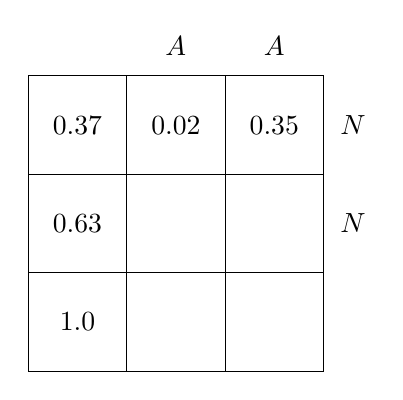
\begin{tikzpicture}[scale=1.25]
\draw (0,0) grid (3,3);
\node at (2.5,3.3) {$\bm{A}$};
\node at (1.5,3.3) {$\bover{A}$};
\node at (3.3,2.5) {$\bm{N}$};
\node at (3.3,1.5) {$\bover{N}$};
\node at (2.5,2.5) {$0.35$};
\node at (0.5,2.5) {$0.37$};
\node at (1.5,2.5) {$0.02$};
\node at (0.5,1.5) {$0.63$};
\node at (0.5,0.5) {$1.0$};
\end{tikzpicture}
\end{center}
בהמשך נתון ש-%
\[
P(\overline{N}\cap\overline{A})=\frac{P(N\cap A)}{5}=\frac{0.35}{5}=0.07\,,
\]
וניתן להשלים את הטבלה:
\begin{center}
\selectlanguage{english}
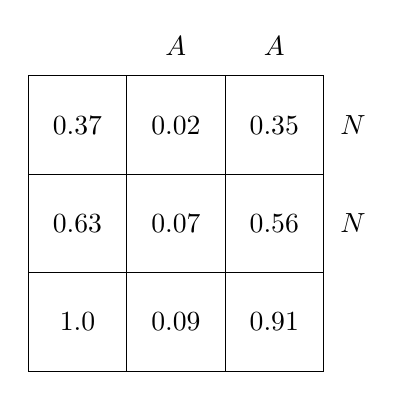
\begin{tikzpicture}[scale=1.25]
\draw (0,0) grid (3,3);
\node at (2.5,3.3) {$\bm{A}$};
\node at (1.5,3.3) {$\bover{A}$};
\node at (3.3,2.5) {$\bm{N}$};
\node at (3.3,1.5) {$\bover{N}$};
\node at (2.5,2.5) {$0.35$};
\node at (0.5,2.5) {$0.37$};
\node at (1.5,2.5) {$0.02$};
\node at (0.5,1.5) {$0.63$};
\node at (0.5,0.5) {$1.0$};
\node at (1.5,0.5) {$0.09$};
\node at (2.5,0.5) {$0.91$};
\node at (1.5,1.5) {$0.07$};
\node at (2.5,1.5) {$0.56$};
\end{tikzpicture}
\end{center}
סעיף א.
\[
P(N/\overline{A})=\frac{P(N\cap \overline{A})}{P(\overline{A})}=\frac{0.02}{0.09}=\frac{2}{9}\,.
\]
סעיף ב. עבור יעל:
\[
P(A/N)=\frac{P(A \cap N)}{P(N)}=\frac{0.35}{0.37}=0.9459\,,
\]
ועבור הדס:
\[
P(A/\overline{N})=\frac{P(A\cap \overline{N})}{P(\overline{N})}=\frac{0.56}{0.63}=0.8889\,.
\]
ליעל הסתברות גבוהה יותר לעבור את המבחן.

סעיף ג. שליש של שש הוא שניים. )שימו לב שלא לקרוא "שלושה" במקום "שליש"!( החישוב הוא לפי נוסחת ברנולי כאשר הערך של
$P(\overline{N}\cap A)$
נמצא בטבלה:
\[
{6 \choose 2}(0.56)^2 (1-0.56)^4=0.1763\,.
\]
סעיף ד. הניסוח "%
\textbf{לפחות אחת}
משתי הטענות
$I, II$"
אומר שהאירוע קורה אם קורה אחד מהאירועים
$I, II$
\textbf{או שניהם}.
באיור להלן שני עגולים המייצגים את שני האירועים
$I, II$.
האירוע "לפחות אחד משניהם" מיוצג על ידי כל השטח המקווקו.
\begin{center}
\selectlanguage{english}
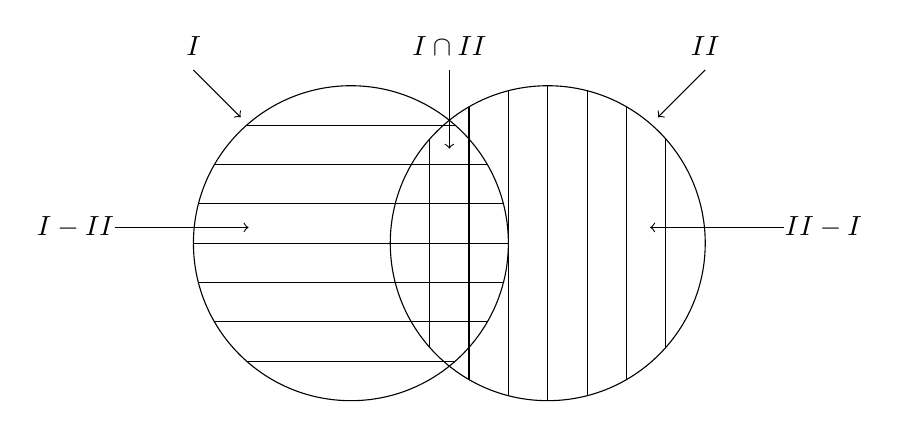
\begin{tikzpicture}
\begin{scope}
\clip[draw] (0,0) circle[radius=2];
\foreach \y in {-1.5,-1,-.5,0,.5,1,1.5}
  \draw (-2,\y) -- (2,\y);
\end{scope}
\begin{scope}
\clip[draw] (2.5,0) circle[radius=2];
\foreach \x in {1,1.5,2,2.5,3,3.5,4}
  \draw (\x,-2) -- (\x,2);
\end{scope}
\node at (-2,2.5) {$I$};
\node at (4.5,2.5) {$II$};
\node at (1.25,2.5) {$I\cap II$};
\node at (-3.5,.2) {$I-II$};
\node at (6,.2) {$II-I$};
\draw[->] (1.25,2.2) -- ++(0,-1);
\draw[->] (-3,.2) -- ++(1.7,0);
\draw[->] (5.5,.2) -- ++(-1.7,0);
\draw[->] (-2,2.2) -- +(.6,-.6);
\draw[->] (4.5,2.2) -- +(-.6,-.6);
\end{tikzpicture}
\end{center}
יש שתי דרכים לחשב את ההסתברות. בדרך הראשונה אנו לוקחים את סכום ההסתברויות של שני האירועים, וחסירים את ההסתברות של האירוע המשותף כי ספרנו אותו פעמיים, פעם כחלק מהאירוע 
$I$
ופעם כחלק מהאירוע
$II$:
\[
P(I \cup II) = P(I) + P(II) - P(I \cap II)\,.
\]
בדרך השניה אנו סופרים כל חלק מהאירוע השותף בנפרד, כאשר הסימון
$A-B$
הוא כל האיברים בקבוצה 
$A$
שאינם בקבוצה
$B$:
\[
P(I \cup II) = P(I-II) + P(II-I) + P(I \cap II)\,.
\]
את ההסתברויות לחישוב ניקח מהטבלה. הדרך הראשונה מופיעה מימין והדרך השניה משמאל:
\begin{center}
\selectlanguage{english}
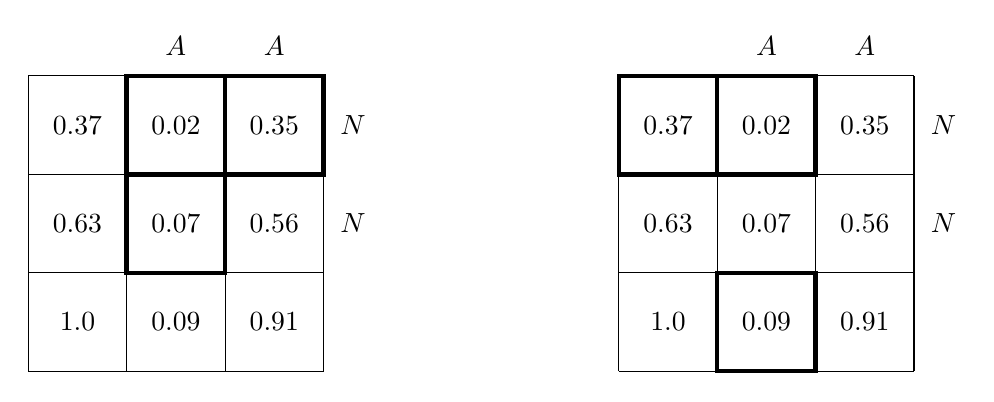
\begin{tikzpicture}[scale=1.25]
\begin{scope}
\draw (0,0) grid (3,3);
\node at (2.5,3.3) {$\bm{A}$};
\node at (1.5,3.3) {$\bover{A}$};
\node at (3.3,2.5) {$\bm{N}$};
\node at (3.3,1.5) {$\bover{N}$};
\node at (2.5,2.5) {$0.35$};
\node at (0.5,2.5) {$0.37$};
\node at (1.5,2.5) {$0.02$};
\node at (0.5,1.5) {$0.63$};
\node at (0.5,0.5) {$1.0$};
\node at (1.5,0.5) {$0.09$};
\node at (2.5,0.5) {$0.91$};
\node at (1.5,1.5) {$0.07$};
\node at (2.5,1.5) {$0.56$};
\draw[ultra thick] (2,2) rectangle +(1,1);
\draw[ultra thick] (1,1) rectangle +(1,1);
\draw[ultra thick] (1,2) rectangle +(1,1);
\end{scope}
\begin{scope}[xshift=6cm]
\draw (0,0) grid (3,3);
\node at (2.5,3.3) {$\bm{A}$};
\node at (1.5,3.3) {$\bover{A}$};
\node at (3.3,2.5) {$\bm{N}$};
\node at (3.3,1.5) {$\bover{N}$};
\node at (2.5,2.5) {$0.35$};
\node at (0.5,2.5) {$0.37$};
\node at (1.5,2.5) {$0.02$};
\node at (0.5,1.5) {$0.63$};
\node at (0.5,0.5) {$1.0$};
\node at (1.5,0.5) {$0.09$};
\node at (2.5,0.5) {$0.91$};
\node at (1.5,1.5) {$0.07$};
\node at (2.5,1.5) {$0.56$};
\draw[ultra thick] (0,2) rectangle +(1,1);
\draw[ultra thick] (1,0) rectangle +(1,1);
\draw[ultra thick] (1,2) rectangle +(1,1);
\end{scope}
\end{tikzpicture}
\end{center}
בשתי הדרכים מקבלים אותה תוצאה:
\[
\renewcommand{\arraystretch}{1.5}
\begin{array}{l}
P(N\cup\overline{A})=P(N) + P(\overline{A}) - P(N\cap\overline{A}) = 0.37+0.09-0.02=0.44\\
P(N\cup\overline{A})=P(N-\overline{A}) + P(\overline{A}-N) + P(N\cap\overline{A}) = 0.35+0.07+0.02=0.44\,.
\end{array}
\]


%%%%%%%%%%%%%%%%%%%%%%%%%%%%%%%%%%%%%%%%%%%%%%%%%%%%%%%%%%%%%%%%%%%

\textbf{\R{
קיץ תשע"ח, מועד ב
}}

\begin{center}
\selectlanguage{english}
%\includegraphics[width=\textwidth]{summer-2018b-3}
\includegraphics[width=.85\textwidth]{summer-2018b-3-1}
\includegraphics[width=\textwidth]{summer-2018b-3-2}
\end{center}

סעיף א
$(1)$.
שחר ידע שהוא ענה נכון על שתי שאלות ולכן כדי לקבל ציון
$60$
עליו לענות על 
\textbf{בדיוק אחת}
משלושת השאלות האחרות:
\[
{3 \choose 1}\left(\frac{1}{4}\right)\left(\frac{3}{4}\right)^2=\frac{27}{64}\,.
\]
סעיף א
$(2)$.
כדי לעבור את המבחן עליו לצבור
\textbf{לפחות}
שלוש תשובות נכונות. יש להוסיף את ההסבתרויות של ארבע וחמש תשובות נכונות:
\[
\frac{27}{64}+{3 \choose 2}\left(\frac{1}{4}\right)^2\left(\frac{3}{4}\right)^1+{3 \choose 3}\left(\frac{1}{4}\right)^3\left(\frac{3}{4}\right)^0=\frac{37}{64}\,.
\]
סעיף ב.
דניאל צירך לענות נכון על שאלה אחת 
\textbf{בדיוק}
מתוך שלושת השאלות הנותרות. דניאל ידע שתשובה אחת מתוך ארבע לא נכונה, לכן ההסתברות שהוא ענה נכון על השאלה היא
$\frac{1}{3}$:
\[
{3 \choose 1}\left(\frac{1}{3}\right)\left(\frac{2}{3}\right)^2=\frac{4}{9}\,.
\]
סעיף ג. אם הדס ידעה ש-%
$k$
מתוך 
$4$
תשובות לא נכונות, ההסתברות שהיא ענתה תשובה נכונה היא
$\frac{1}{4-k}$,
וההסתברות שהיא תענה תשובה לא נכונה היא
$\frac{4-k-1}{4-k}$.
כדי לקבל ציון 
\textbf{בדיוק}
$100$
הדס צריכה לבחור תשובות נכונות לשתי השאלות הנותרות. כדי לקבל ציון 
\textbf{בדיוק}
$60$
עליה לבחר תשובות לא נכונות לשתי השאלות הנותרות.

אין צורך להשתמש בנוסחת ברנולי במלואו, כי כאשר מחשבים את ההסתברות של "כל" או "אף אחד", 
${n\choose k}=1$,
וגם
$(1-p)^0=1$
או
$p^0=1$.
לכן, מספיק לחשב את ההסתברות של האירוע לחזקת מספר השאלות:
\begin{eqnarray*}
\left(\frac{1}{4-k}\right)^2 &=&\left(\frac{4-k-1}{4-k}\right)^2\\
(3-k)^2&=&1\\
k^2-6k+8&=& 0\,.
\end{eqnarray*}
הפתרונות הם 
$k=2,4$
אבל נתון ש-"אחת ]מהתשובות[ נכונה", לכן הפתרון היחיד הוא
$k=2$.

%%%%%%%%%%%%%%%%%%%%%%%%%%%%%%%%%%%%%%%%%%%%%%%%%%%%%%%%%%%%%%%%%%%

\newpage

\textbf{\R{
חורף תשע"ז
}}

\begin{center}
\selectlanguage{english}
\includegraphics[width=.95\textwidth]{winter-2017-3.png}
\end{center}
\vspace{-1ex}

סעיף א. לפי המידע הנתון:
\[
{5 \choose 4} p^4(1-p)^1 = 3{5\choose 5}p^5(1-p)^0\,.
\]
והפתרון הוא
$p=\frac{5}{8}$.

סעיף ב. ההסתברות ל-%
$3,4,5$
פגיעות היא:
\[
{5 \choose 3}p^3(1-p)^2 + {5 \choose 4}p^4(1-p)^1 + {5 \choose 5}p^5(1-p)^0
\]
נציב
$p=\frac{5}{8}$
ונקבל
$0.7248$.

סעיף ג 
$(1)$.
לדעתי, ניסוח השאלה לא ברור. אני פירשתי אותה: מה ההסתברות של
\textbf{האירוע}
"אביגיל מחטיאה בזריקה השנייה ופוגעת בשלוש או ארבע מהזריקות האחרות"? כותב הבחינה התכוון להסתברות מותנית: "%
\textbf{אם ידוע ש-}%
אביגיל החטיאה בזריקה השנייה, מה ההסתברות שהיא פוגעת בשלוש או ארבע מהזריקות האחרות"?
\[
\renewcommand{\arraystretch}{2}
\begin{array}{c}
P(1,3,4,5\ \textrm{\R{אביגיל פגעה בשלוש או ארבע מהזריקות}}/\textrm{\R{אביגיל החטיאה בזריקה השניה}}) =\\
\displaystyle\frac{P(1,3,4,5\ \textrm{\R{אביגיל פגעה בשלוש או ארבע מהזריקות}}\cap \textrm{\R{אביגיל החטיאה בזריקה השניה}})}{P(\textrm{\R{אביגיל החטיאה בזריקה השניה}})}\,.
\end{array}
\]
אפשר לפתור את הבעיה בשתי דרכים. נתחיל עם הדרך הפשוטה יותר. נתון שהסיכוי לפגוע במטרה אינו תלוי בניסיונות הקודמים, ולכן ההסתברויות בלתי תלויות והחישוב מצטמצם:
\[
\renewcommand{\arraystretch}{2}
\begin{array}{c}
\displaystyle\frac{P(1,3,4,5\ \textrm{\R{אביגיל פגעה בשלוש או ארבע מהזריקות}}) \cdot P(\textrm{\R{אביגיל החטיאה בזריקה השניה}})}{P(\textrm{\R{אביגיל החטיאה בזריקה השניה}})}=\\
P(1,3,4,5\ \textrm{\R{אביגיל פגעה בשלוש או ארבע מהזריקות}})\,.
\end{array}
\]
החישוב הוא:
\[
{4\choose 4}\left(\frac{5}{8}\right)^4 \left(\frac{3}{6}\right)^0 +{4\choose 3}\left(\frac{5}{8}\right)^3\left(\frac{3}{8}\right)^1 = 0.5188\,.
\]
הדרך השנייה ארוכה יותר אבל מעניינת. האירוע של החיתוך בנוסחה להסתברות מותנית מורכבת משני אירועים: )א( לא משנה מה יצאה מהזריקה הראשונה, הזריקה השניה החטיאה, ושלושת הזריקות האחרונות פגעו. )ב( הזריקה הראשונה פגעה, הזריקה השניה החטיאה, ושתיים מתוך שלושת הזריקות האחרונות פגעו. הסתברות של האירוע המשותף היא:
\[
1\cdot \frac{3}{8} \cdot \left(\frac{5}{8}\right)^3 \quad + \quad
\frac{5}{8}\cdot \frac{3}{8} \cdot \left[{3\choose 2}\left(\frac{5}{8}\right)^2\frac{3}{8}\right] = 0.1945\,.
\]
נחלק ב-%
$\frac{3}{8}$,
ההסתברות האביגיל החטיאה בזריקה השנייה, ונקבל 
$0.5188$.

סעיף ג 
$(2)$.
לא משנה איזו זריקה החטיאה, הזריקות בלתי תלויות וחישוב ההסתברות של "תמר פגעה בשלוש  או ארבע מהזריקות 
$2,3,4,5$"
נותן אותה תוצאה כמו האירוע "אביגיל פגעה בשלוש או ארבע מהזריקות 
$1,3,4,5$".

%%%%%%%%%%%%%%%%%%%%%%%%%%%%%%%%%%%%%%%%%%%%%%%%%%%%%%%%%%%%%%%%%%%
\bigskip

\textbf{\R{
קיץ תשע"ז, מועד א
}}

\begin{center}
\selectlanguage{english}
\includegraphics[width=.95\textwidth]{summer-2017a-3}
\end{center}

סעיף א. נסמן ב-%
$D$
את האירוע "לדייר יש קלנועית" ואת ההסתברות של האירוע ב-%
$p$.
נתון ש:
\[
{9\choose 4} p^4 (1-p)^5=24 {9\choose 6} p^6 (1-p)^3\,.
\]
נפשט ונקבל משוואה ריבועית:
\[
15p^2+2p-1=0\,,
\]
עם שני פתרונות
$p=\frac{1}{5},-\frac{1}{3}$.
הסתברות חייבת להיות לא-שלילית ולכן התשובה היא 
$p=\frac{1}{5}=0.2$.

סעיף ב. המילים
"\textbf{ידוע ש-}"
מכוונות להסתברות מותנית:
\[
P(D=4/D\ge3) = \frac{P(D=4\cap D\ge 3)}{P(D\ge 3)}\,.
\]
כאשר יש חפיפה בין שני ביטויים בחיתוך אפשר לפשט אותו. ברור שאם ערך גדול או שווה
$3$
\textbf{וגם}
שווה ל-%
$4$
אז הוא שווה ל-%
$4$:
\[
P(D=4/D\ge3) =\frac{P(D=4)}{P(D\ge 3)}\,.
\]
לפי נוסחת ברנולי:
\[
P(D=4)={6\choose 4} 0.2^4 (1-0.2)^2= 0.01536\,.
\]
את הערך של
$P(D\ge 3)$
אפשר לחשב בשתי דרכים, בצורה ישירה או כאחד פחות המשלים. נבחר את האפשרות השנייה כי יש פחות גורמים בביטוי:
\[
1-0.2^0(1-0.2)^6-{6\choose 1}0.2^1(1-0.2)^5 - {6 \choose 2} 0.2^2(1-0.2)^4=0.099\,,
\]
והתשובה היא
$\displaystyle\frac{0.01536}{0.099}=0.15534$.

סעיף ג. הבחירה 
\textbf{האחרונה} 
תהיה "הצלחה" ויהיו שתי "הצלחות" בחמשת הבחירות הקודמות:
\[
\overbrace{\pm\;\pm\;\pm\;\pm\;\pm}^{2/5}\quad\quad \overbrace{+}^{1/1}\,.
\]
התשובה מתקבלת מנוסחת ברנולי לבחירות הראשונות כפול ההסתברות
$p$
לבחירה האחרונה:
\[
\left[{5\choose 2}0.2^2 (1-.02)^3\right]\cdot 0.2=0.04096\,.
\]

%%%%%%%%%%%%%%%%%%%%%%%%%%%%%%%%%%%%%%%%%%%%%%%%%%%%%%%%%%%%%%%%%%%
\newpage

\textbf{\R{
קיץ תשע"ז, מועד ב
}}

\begin{center}
\selectlanguage{english}
\includegraphics[width=.95\textwidth]{summer-2017b-3}
\end{center}

המילים "מוציאים באקראי
$\ldots$
\textbf{ולאחר מכן}
שוב מוציאים באקראי" מכוונות לשימוש בעץ. נסמן ב-%
\textsf{b}
את מספר הכדורים הכחולים בקופסה 
$I$.
באיור~%
\L{\ref{fig.summer-2017b.1}},
בכל צומת רשום שני זוגות של מספרים: מספר הכדורים האדומים ומספר הכדורים הכחולים בקופסה
$I$,
ומתחתיו מספר הכדורים האדומים ומספר הכדורים הכחולים בקופסה
$II$.

סעיף א. הכוכביות מסמנות את שתי האפשרויות בהן הוצאנו כדור אדום אחד בדיוק מקופסה
\textsf{I}.
\begin{figure}
\begin{center}
\selectlanguage{english}
\begin{tikzpicture}
[grow=right,
level 1/.append style={font=\sffamily,text width=2cm,level distance=5cm,sibling distance=10em},
level 2/.append style={font=\sffamily,text width=2cm,level distance=7cm,sibling distance=6em}]
\node[font=\sffamily,text width=2cm] {(10-b,b)\\(3,7)} % root
child {
  node {(10-b,b)\\(3,7)}
    child {
      node {(10-b,b)\\(3,7)}
      edge from parent node[below] {\R{כחול}}
        node[above,xshift=16mm,yshift=-2mm] {$\frac{b}{10}$}
    }
    child {
      node {(9-b,b)\ *\\(4,7)}
      edge from parent node[above] {\R{אדום}}
        node[below,xshift=16mm,yshift=2mm] {$\frac{10-b}{10}$}
    }
    edge from parent node[below] {\R{כחול}} node[above,xshift=8mm,yshift=0mm] {$\frac{b}{10}$}
}
child { 
  node {(9-b,b)\\(4,7)}
    child {
      node {(9-b,b)\ *\\(4,7)}
      edge from parent node[below] {\R{כחול}}
        node[above,xshift=16mm,yshift=-2mm] {$\frac{b}{9}$}
    }
    child {
      node {(8-b,b)\\(5,7)}
      edge from parent node[above] {\R{אדום}}
        node[below,xshift=16mm,yshift=2mm] {$\frac{9-b}{9}$}
    }
    edge from parent node[above] {\R{אדום}} 
      node[below,xshift=8mm,yshift=0mm] {$\frac{10-b}{10}$}
};
\end{tikzpicture}
\selectlanguage{hebrew}
\setlength{\belowcaptionskip}{-4ex}
\caption{עץ ההסתברויות של הוצאת הכדורים מקופסה $I$}\label{fig.summer-2017b.1}
\end{center}
\end{figure}
נשווה את הסתברות הנתונה לסכום ההסתברויות של שני המסלולים:
\[
\frac{10-b}{10}\cdot\frac{b}{9} + \frac{b}{10}\cdot\frac{10-b}{10} = \frac{19}{36}\,.
\]
נפשט ונקבל משוואה ריבועית 
$b^2-10b+25=0$
שיש לה פתרון אחד
$b=5$.

סעיף ב. לאחר הצבת 
$b=5$,
נקבל עבור כל מצב את מספר הכדורים האדומים וכחולים בקופסה
$II$,
נוכל לחשב את ההסתברויות להוצאת כדור אדום מקופסה
$II$,
ונסכם את ההסתברויות לאחר הכפלתן בהסתברות להגיע לכל אחד מהמצבים:
\[
\renewcommand{\arraystretch}{2}
\begin{array}{l}
\displaystyle\left(\frac{5}{10}\cdot\frac{4}{9}\right)\left(\frac{5}{5+7}\right)+
\left(\frac{5}{10}\cdot\frac{5}{9}\right)\left(\frac{4}{4+7}\right)+\\
\displaystyle\left(\frac{5}{10}\cdot\frac{5}{10}\right)\left(\frac{4}{4+7}\right)+
\left(\frac{5}{10}\cdot\frac{5}{10}\right)\left(\frac{3}{3+7}\right)
=0.3595\,.
\end{array}
\]

סעיף ג. המילים 
"\textbf{ידוע ש-}"
מכוונת להסתברות מותנית:
\vspace{-4ex}
\[
\renewcommand{\arraystretch}{2}
\begin{array}{c}
P(II\ \textrm{\R{נשארו שלושה אדומים בקופסה}}/II\ \textrm{\R{הוציאו כדור אדום מקופסה}}) =\\
\displaystyle\frac{P(II\ \textrm{\R{נשארו שלושה אדומים בקופסה}} \cap II\ \textrm{\R{הוציאו כדור אדום מקופסה}})}{P(II\ \textrm{\R{הוציאו כדור אדום מקופסה}})}
\end{array}
\]
ישארו שלושה כדורים אדומים רק אם היו אברעה כדורים אדומים לפני הבחירה. ההסתברות במנה היא ההסתברות )הנתונה!( שנגיע לאחד המצבים המסומנים בכוכבית כפול ההסתברות לבחור אדום מקופסה 
$II$,
וחישבנו את ההסתברות במכנה בסעיף ב. התשובה היא:
\[
\frac{\displaystyle\frac{19}{36}\cdot\frac{4}{11}}{0.3595}=0.53385\,.
\]

%%%%%%%%%%%%%%%%%%%%%%%%%%%%%%%%%%%%%%%%%%%%%%%%%%%%%%%%%%%%%%%%%%%
\newpage

\textbf{\R{
חורף תשע"ו
}}

\begin{center}
\selectlanguage{english}
\includegraphics[width=.85\textwidth]{winter-2016-3}
\end{center}
סעיף א. ההסתברות שדן לא יזכה באף אחד מחמישת המשחקים היא 
$P(0)^5$.
נתון שערך זה הוא 
$\frac{1}{32}$,
ולכן 
$P(0)=\frac{1}{2}$.
לפי המידע הנתון:
\begin{eqnarray*}
{5\choose 2} P(50)^2 (1-P(50))^3 &=& {5\choose 1} P(50) (1-P(50))^4\\
P(50)&=&\frac{1}{3}\,.
\end{eqnarray*}
סעיף ב. לפי ההסתברות המשלימה:
$\displaystyle P(100) = 1 - P(0) - P(50) = 1-\frac{1}{2}-\frac{1}{3}=\frac{1}{6}$.

סעיף ג. המילים
"\textbf{ידוע כי}"
מכוונות להסתברות מותנית:
\vspace{-4ex}
\[
\renewcommand{\arraystretch}{2}
\begin{array}{c}
P(\textrm{\R{ באף משחק}}50\textrm{\R{לא זכה ב-}}
/
\textrm{\R{ בשני משחקים}}
100\textrm{\R{זכה ב-}}) =\\
\displaystyle\frac{
P(\textrm{\R{ באף משחק}}50\textrm{\R{לא זכה ב-}}
\cap
\textrm{\R{ בשני משחקים}}
100\textrm{\R{זכה ב-}})
}
{P(
\textrm{\R{ בשני משחקים}}
100\textrm{\R{זכה ב-}})}\,.
\end{array}
\]
נתבונן בעץ המציג את תוצאות שני המשחקים )איור~%
\L{\ref{fig.winter-2017.1}}(.
סימנו את המסלולים שבהם דן זכה ב-%
$100$
והמסלולים בהם דן לא זכה ב-%
$50$
באף אחד משני המשחקים.
\begin{figure}
\begin{center}
\selectlanguage{english}
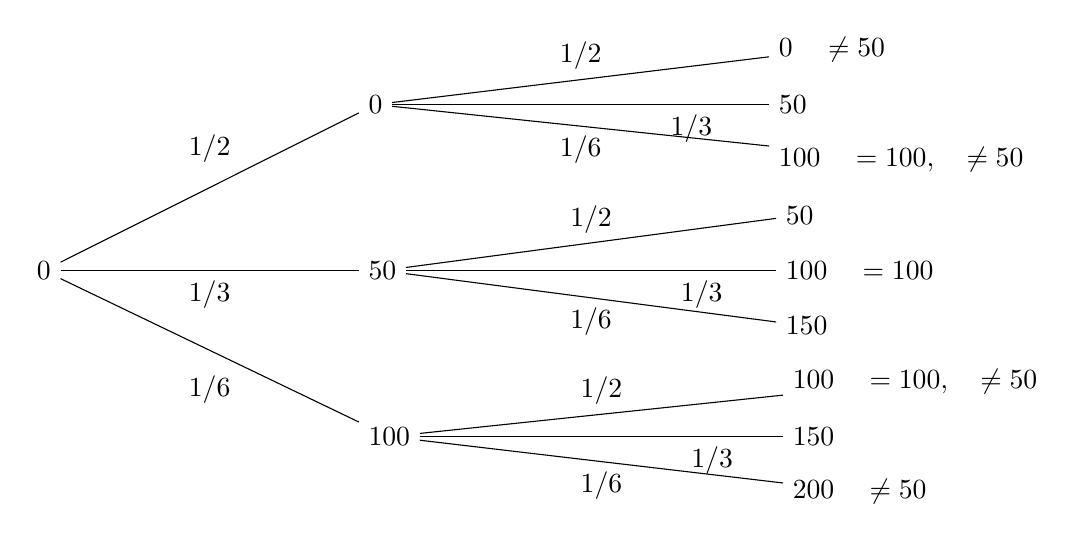
\begin{tikzpicture}
[grow=right,
level 1/.append style={font=\sffamily,level distance=4cm,sibling distance=6em},
level 2/.append style={font=\sffamily,level distance=5cm,sibling distance=2em}]
\node[left] {$0$} % root
child {
  node[right] {$100$}
    child {
      node[right] {$200\quad \neq 50$}
      edge from parent node[below] {$1/6$}
    }
    child {
      node[right] {$150$}
      edge from parent node[below,xshift=4em] {$1/3$}
    }
    child {
      node[right] {$100\quad =100,\quad \neq 50$}
      edge from parent node[above] {$1/2$}
    }
    edge from parent node[below,yshift=-2mm] {$1/6$}
}
child {
  node[right] {$50$}
    child {
      node[right] {$150$}
      edge from parent node[below] {$1/6$}
    }
    child {
      node[right] {$100\quad =100$}
      edge from parent node[below,xshift=4em] {$1/3$}
    }
    child {
      node[right] {$50$}
      edge from parent node[above] {$1/2$}
    }
    edge from parent node[below] {$1/3$}
}
child {
  node[right] {$0$}
    child {
      node[right] {$100\quad =100,\quad \neq 50$}
      edge from parent node[below] {$1/6$}
    }
    child {
      node[right] {$50$}
      edge from parent node[below,xshift=4em] {$1/3$}
    }
    child {
      node[right] {$0\quad \neq 50$}
      edge from parent node[above] {$1/2$}
    }
    edge from parent node[above,yshift=2mm] {$1/2$}
}
;
\end{tikzpicture}
\selectlanguage{hebrew}
\setlength{\belowcaptionskip}{-6ex}
\caption{עץ ההסתברויות של המשחקים}\label{fig.winter-2017.1}
\end{center}
\end{figure}
חישוב ההסתברות המותנית:
\[
\frac{\displaystyle\frac{1}{2}\cdot\frac{1}{6} + \frac{1}{6}\cdot \frac{1}{2}}{\displaystyle\frac{1}{2}\cdot\frac{1}{6} + \frac{1}{3}\cdot \frac{1}{3}+ \frac{1}{6}\cdot \frac{1}{2}}  =  \frac{\displaystyle\frac{1}{6}}{\displaystyle\frac{5}{18}}=\frac{3}{5}\,.
\]

%%%%%%%%%%%%%%%%%%%%%%%%%%%%%%%%%%%%%%%%%%%%%%%%%%%%%%%%%%%%%%%%%%%
\newpage

\textbf{\R{
קיץ תשע"ו, מועד א
}}

\begin{center}
\selectlanguage{english}
\includegraphics[width=.95\textwidth]{summer-2016a-3}
\end{center}

נסמן 
$=S$
נבחנים שהצליחו,
$=K$
נבחנים מקיבוצים,
$=M$
נבחנים ממושבים,
$=E$
נבחנים מערים. ההסתברויות הנתונות הן:
\[
P(K)=0.20,\;P(M)=0.40,\;P(E)=0.40,\;P(S)=0.70\,.
\]
נחשב את שאר ההסתברויות. לפי הסתברות משלימה
$P(\overline{S})=1-P(S)=0.30$.
נתון:
\[
P(\overline{S}/M)=P(\overline{S}\cap M) / P(M)=\frac{1}{8}\,,
\]
ולכן:
\[
P(\overline{S}\cap M)=\frac{1}{8}P(M)=0.05\,.
\]
לפי ההגדרה:
\[
P(S)=P(K\cap S) + P(M\cap S) + P(E\cap S)\,.
\]
נסמן
$P(K\cap S)=p$,
ההסתברות שנבחנים מקיבוצים הצליחו. נתון:
\[
P(E\cap S)=2.5P(K\cap S)=2.5p\,,
\]
ולכן:
\[
0.70=p+(0.40-0.05)+2.5p\,,
\]
ו-%
$p=0.1$.

שימו לב שהמילים 
"$\frac{1}{8}$
\textbf{מן}
הנבחנים שהיו ממושבים נכשלו" מכוונות להסתברות מותנית, לעומת המילים "ההסתברות לבחור באקראי
\textbf{מבין כל}
הנבחנים נבחן שהיה מהעיר
\textbf{וגם}
הצליח במבחן" מכוונות לחיתוך הסתברויות. המילה "מבין" בדרך כלל מכוונת להסתברות מותנית, אבל כאשר "מבין" מתייחס ל-%
"\textbf{כל}
הנבחנים" אין הסתברות מותנית. לחילופין, ההסתברות לבחור אחד "מכל הנבחנים" היא 
$1$,
ולכן:
\[
P(E\cap S/\textrm{\R{כל הנבחנים}})=
\frac{(P(E\cap S)\cap \textrm{\R{כל הנבחנים}})}
{P(\textrm{\R{כל הנבחנים}})} = 
\frac{P(E\cap S)}{1}=P(E\cap S)\,.
\]
נסכם את המידע בטבלה:
\begin{center}
\selectlanguage{english}
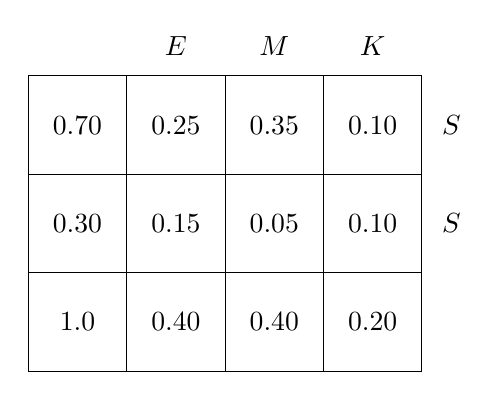
\begin{tikzpicture}[scale=1.25]
\draw (0,0) grid (4,3);
\node at (3.5,3.3) {$\bm{K}$};
\node at (2.5,3.3) {$\bm{M}$};
\node at (1.5,3.3) {$\bm{E}$};
\node at (4.3,2.5) {$\bm{S}$};
\node at (4.3,1.5) {$\bover{S}$};

\node at (0.5,2.5) {$0.70$};
\node at (0.5,1.5) {$0.30$};
\node at (0.5,0.5) {$1.0$};

\node at (1.5,2.5) {$0.25$};
\node at (1.5,1.5) {$0.15$};
\node at (1.5,0.5) {$0.40$};

\node at (2.5,2.5) {$0.35$};
\node at (2.5,1.5) {$0.05$};
\node at (2.5,0.5) {$0.40$};

\node at (3.5,2.5) {$0.10$};
\node at (3.5,1.5) {$0.10$};
\node at (3.5,0.5) {$0.20$};
\end{tikzpicture}
\end{center}
סעיף א. לפי הנוסחה להסתברות מותנית:
\[
P(\overline{E}/\overline{S})=P((K\cup M)/\overline{S}) = \frac{P(K\cap \overline{S})+P(M\cap \overline{S})}{P(\overline{S})}=\frac{0.10+0.05}{0.30}=\frac{1}{2}\,.
\]
סעיף ב
$(1)$.
לפי הנוסחה להסתברות מותנית:
\[
P(\overline{M}/S)=P((K\cup E)/S) = \frac{P(K\cap S)+P(E\cap S)}{P(S)}=\frac{0.10+0.25}{0.70}=\frac{1}{2}\,.
\]
סעיף ב
$(2)$.
%את ההסתברות שנבחן שהצליח המושב ניתן לחשב בדיוק כמו בסעיף ב
%$(1)$,
%אבל ההסתברות זו היא המשלים של ההסתברות שחושב שם
%$P(M/S)=1-P(\overline{M}/S)=1-\frac{1}{2}=\frac{1}{2}$.
"לפחות אחד ממושב" הוא המשלים ל-"כולם לא מהמושב":
\[
1-P(\overline{M}/S)^5=1-\left(\frac{1}{2}\right)^2=\frac{31}{32}\,.
\]
%%%%%%%%%%%%%%%%%%%%%%%%%%%%%%%%%%%%%%%%%%%%%%%%%%%%%%%%%%%%%%%%%%%
\newpage

\textbf{\R{
קיץ תשע"ו, מועד ב
}}

\begin{center}
\selectlanguage{english}
\includegraphics[width=.86\textwidth]{summer-2016b-3}
\end{center}
נסמן:
$=y$
ההסתברות שיעל תנצח במשחק בודד, 
$=a$
ההסתברות שאנה תנצח במשחק בודד.

סעיף א. לפי המידע הנתון:
\[
{4 \choose 2}y^2(1-y)^2 + {4\choose 3}y^3(1-y) = 10\cdot {4\choose 4}y^4(1-y)^0\,.
\]
נפשט ונקבל משוואה ריבועית
$4y^2+4y-3=0$
שהשורש החיובי היחיד שלה היא
$y=\frac{1}{2}$.

סעיף ב. כדאי לצייר עץ של האירועים, אבל אוותר עליו בשאלה זו כי המצב פשוט. האפשרויות לקבל שוויון הן: )א( ניצחון אחד לאנה וליעל, או )ב( תיקן בשני המשחקים. ההסתברות לתיקו היא המשלים לסכום ההסתברויות שאחת מהן תנצח:
\[
{2 \choose 1}ya + (1-(y+a))^2 = 0.34\,.
\]
נציב 
$y=\frac{1}{2}$
ונקבל
$a=0.3$.

סעיף ג. המילים
"\textbf{אם ידוע ש-}"
מכוונות להסתברות מותנית:
\vspace{-2ex}
\[
\renewcommand{\arraystretch}{2}
\begin{array}{c}
P(\textrm{\R{אנה תנצח במשחק השני}} / \textrm{\R{תוצאת הסבב השני היא שוויון}})=\\
\displaystyle\frac{
P(\textrm{\R{אנה תנצח במשחק השני}} \cap \textrm{\R{תוצאת הסבב השני היא שוויון}})
}
{P(\textrm{\R{תוצאת הסבב השני היא שוויון}})}\,.
\end{array}
\]
ההסתברות לשיוון בסבב השני נתונה. אם אנה תנצח במשחק השני, יהיה שוויון רק אם גם יעל תנצח במשחק הראשון:
\vspace{-1ex}
\[
\frac{ya}{.34}=\frac{\displaystyle\frac{1}{2}\cdot 0.3}{.34}=0.4412\,.
\]
שימו לב שלא צריכים
$2 \choose 1$
כי האירוע הוא שאנה תנצח במשחק 
\textbf{השני}
ויעל תנצח במשחק
\textbf{הראשון}.
%%%%%%%%%%%%%%%%%%%%%%%%%%%%%%%%%%%%%%%%%%%%%%%%%%%%%%%%%%%%%%%%%%%
\newpage

\textbf{\R{
חורף תשע"ה
}}

\begin{center}
\selectlanguage{english}
\includegraphics[width=.85\textwidth]{winter-2015-3}
\end{center}

"יישוב גדול" אומר לי שניתן לבחור מספר רב של תושבים, לפחות שמונה תושבים כפי שנדרש.

סעיף א. כל קבוצה היא בחירה בלתי תלוייה:
\[
{4 \choose 2}\left(\frac{2}{3}\right)^2\left(1-\frac{2}{3}\right)^2=\frac{8}{27}\,,
\]
וכדי לקבל את ההסתברות שלשתי הקבוצות יהיו בדיוק שני גברים, נעלה ערך זה בריבוע:
\[
\left(\frac{8}{27}\right)^2=\frac{64}{729}\,.
\]
סעיף ב. המילים
"\textbf{ידוע כי}"
מכוונות להסתברות מותנית:
\vspace{-4ex}
\[
\renewcommand{\arraystretch}{2}
\begin{array}{c}
P(\textrm{\R{בדיוק שני גברים}} / \textrm{\R{לכל היותר שני גברים}})=\\
\displaystyle\frac{
P(\textrm{\R{בדיוק שני גברים}} \cap \textrm{\R{לכל היותר שני גברים}})
}
{P(\textrm{\R{לכל היותר שני גברים}})}\,.
\end{array}
\]
החיתוך במנה שקולה ל-"בדיוק שני גברים" )שחישבנו בסעיף א(, כי "לכל היותר שני גברים" היא 
$0,1,2$
גברים. "לכל היותר שני גברים" הוא הסכום של שלוש נוסחאות ברנולי:
\[
\left(\frac{2}{3}\right)^0\left(\frac{1}{3}\right)^4 + {4\choose 1}\left(\frac{2}{3}\right)^1\left(\frac{1}{3}\right)^3 + {4\choose 2}\left(\frac{2}{3}\right)^2\left(\frac{1}{3}\right)^2=\frac{11}{27}\,
\]
והתשובה לשאלה היא:
\[
\frac{8/27}{11/27}=\frac{8}{11}\,.
\]

%%%%%%%%%%%%%%%%%%%%%%%%%%%%%%%%%%%%%%%%%%%%%%%%%%%%%%%%%%%%%%%%%%%
\newpage

\textbf{\R{
קיץ תשע"ה, מועד א
}}

\begin{center}
\selectlanguage{english}
\includegraphics[width=.85\textwidth]{summer-2015a-3}
\end{center}

נסמן 
$=n$
מספר הספרות בקבוצה. מספר הזוגיים 
$3=$,
ומספר האי-זוגיים
$n-3=$.
השאלה מתארת בחירה של "הספרה הראשונה" ואחר כך "הספרה הראשונה", תיאור המכוון לעץ הסתברויות )איור~%
\L{\ref{fig.summer-2015a.1}}(.
כדי לפשט את האיור רשמתי בכל צומת את ההסתברויות ולא את מספר הספרות.

\begin{figure}[H]
\begin{center}
\selectlanguage{english}
\begin{tikzpicture}
[grow=right,
level 1/.append style={text width=2cm,level distance=3.5cm,sibling distance=8em},
level 2/.append style={text width=2.5cm,level distance=4.5cm,sibling distance=4em}]
\node[text width=2cm] {$\left(\frac{3}{n},\frac{n-3}{n}\right)$} % root
child {
  node {$\left(\frac{3}{n-1},\frac{n-4}{n-1}\right)$}
    child {
      node {$\left(\frac{3}{n-2},\frac{n-5}{n-2}\right)\quad *$}
      edge from parent node[below,xshift=5mm,yshift=-1mm] {\R{אי-זוגי}}
    }
    child {
      node {$\left(\frac{2}{n-2},\frac{n-4}{n-2}\right)$}
      edge from parent node[above,xshift=5mm,yshift=1mm] {\R{זוגי}}
    }
    edge from parent node[below,yshift=-1mm] {\R{אי-זוגי}}
}
child { 
  node {$\left(\frac{2}{n-1},\frac{n-3}{n-1}\right)$}
    child {
      node {$\left(\frac{2}{n-2},\frac{n-4}{n-2}\right)\quad *$}
      edge from parent node[below,xshift=5mm,yshift=-1mm] {\R{אי-זוגי}}
    }
    child {
      node {$\left(\frac{1}{n-2},\frac{n-3}{n-2}\right)$}
      edge from parent node[above,xshift=5mm,yshift=1mm] {\R{זוגי}}
    }
    edge from parent node[above] {\R{זוגי}}
};
\end{tikzpicture}
\selectlanguage{hebrew}
\setlength{\belowcaptionskip}{-8ex}
\caption{עץ ההסתברויות של בחירת הספרות}\label{fig.summer-2015a.1}
\end{center}
\end{figure}

סעיף א. המספר יהיה אי-זוגי אם 
\textbf{הבחירה השנייה}
היא של ספרה אי-זוגית. המסלולים האלה מסומנים בכוכביות באיור. נשווה את סכום ההסתברויות של המסלולים לערך הנתון:
\[
\frac{3}{n}\cdot\frac{n-3}{n-1} \;+\; \frac{n-3}{n}\cdot\frac{n-4}{n-1} = \frac{4}{7}\,.
\]
נפשט ונקבל משוואה ריבועית
$n^2-8n+7=0$
שיש לה שני פתרונות לא-שליליים
$n=1,n=7$.
נתון שיש לפחות שלוש ספרות, לכן מספר הספרות הוא
$7$.
שימו לב שהשאלה מבקשת את מספר הספרות 
\textbf{האי-זוגיות}
ולכן התשובה היא
$7-3=4$.

סעיף ב. המילים 
"\textbf{אם ידוע ש-}"
מכוונות להסתברות מותנית. במספר זוגי הספרה האחרונה זוגית:
\vspace{-3ex}
\[
\renewcommand{\arraystretch}{2}
\begin{array}{c}
P(\textrm{\R{שתי ספרות זוגיות}} / \textrm{\R{ספרה אחרונה זוגית}})=\\
\displaystyle\frac{
P(\textrm{\R{שתי ספרות זוגיות}} \cap \textrm{\R{ספרה אחרונה זוגית}})
}
{P(\textrm{\R{ספרה אחרונה זוגית}})}=\\
\displaystyle\frac{
P(\textrm{\R{שתי ספרות זוגיות}})
}
{P(\textrm{\R{ספרה אחרונה זוגית}})}\,.
\end{array}
\]
את החיתוך אפשר לפשט כי אם שתי הספרות זוגיות, הספרה האחרונה חייבת להיות זוגית.

ניתן לחשב את ההסתברות "ספרה אחרונה זוגית" במכנה לפי המידע בעץ ההסתברויות או פשוט לשים לב שהיא המשלימה לערך הנתון בסעיף א של "הספרה האחרונה אי-זוגית". נחשב את ההסתברות במנה לפי המסלול הבודד בעץ ההסתברויות )איור~
\L{\ref{fig.summer-2015a.2}}(
של בחירה של שתי ספרות זוגיות:
\[
\frac{\displaystyle\frac{3}{7}\cdot\frac{2}{6}}{1-\displaystyle\frac{4}{7}}=\frac{1}{3}\,.
\]
סעיף ג. הסכום יהיה זוגי רק אם שתי הספרות האחרונת הן זוגיות או אי-זוגיות:
\begin{eqnarray*}
2k_1+2k_2+2k_3&=&2(k_1+k_2+k_3)\\
2k_1+2(k_2+1)+2(k_3+1)&=&2(k_1+k_2+k_3+1)\,.
\end{eqnarray*}
שני האירועים )בחירת הספרות( בלתי תלויים, ולכן אפשר לבטא את החיתוך כמכפלה:
\vspace{-3ex}
\[
\renewcommand{\arraystretch}{2}
\begin{array}{c}
P(\textrm{\R{סכום זוגי}} / \textrm{\R{ספרה ראשונה זוגית}})=\\
\displaystyle\frac{
P(\textrm{\R{סכום זוגי}} \cap \textrm{\R{ספרה ראשונה זוגית}})
}
{P(\textrm{\R{ספרה ראשונה זוגית}})}=\\
\displaystyle\frac{
P(\textrm{\R{סכום זוגי}}) \cdot P(\textrm{\R{ספרה ראשונה זוגית}})
}
{P(\textrm{\R{ספרה ראשונה זוגית}})}=\\
P(\textrm{\R{סכום זוגי}})\,.
\end{array}
\]
שימו לב שלאחר הבחירה הראשונה של אמילי מספר הספרות הוא שש. לפי עץ ההסתברויות החדש )איור~
\L{\ref{fig.summer-2015a.3}}(
 ההסתברות היא:
\[
\frac{2}{6}\cdot\frac{1}{5}+\frac{4}{6}\cdot\frac{3}{5}=\frac{7}{15}\,.
\]

\begin{figure}[H]
\begin{center}
\selectlanguage{english}
\begin{tikzpicture}
[grow=right,
level 1/.append style={level distance=3cm,sibling distance=8em},
level 2/.append style={level distance=4cm,sibling distance=4em}]
\node {$\left(\frac{3}{7},\frac{4}{7}\right)$} % root
child {
  node {$\left(\frac{3}{6},\frac{3}{6}\right)$}
    child {
      node {$\left(\frac{3}{5},\frac{2}{5}\right)$}
      edge from parent node[below,xshift=5mm,yshift=-3mm] {\R{אי-זוגי}}
    }
    child {
      node {$\left(\frac{2}{5},\frac{3}{5}\right)$}
      edge from parent node[above,xshift=5mm,yshift=1mm] {\R{זוגי}}
    }
    edge from parent node[below,yshift=-3mm] {\R{אי-זוגי}}
}
child { 
  node {$\left(\frac{2}{6},\frac{4}{6}\right)$}
    child {
      node {$\left(\frac{2}{5},\frac{3}{5}\right)$}
      edge from parent node[below,xshift=5mm,yshift=-3mm] {\R{אי-זוגי}}
    }
    child {
      node {$\left(\frac{1}{5},\frac{4}{5}\right)\quad$ *}
      edge from parent node[above,xshift=5mm,yshift=1mm] {\R{זוגי} }
    }
    edge from parent node[above,yshift=2mm] {\R{זוגי}}
};
\end{tikzpicture}
\selectlanguage{hebrew}
\caption{עץ ההסתברויות של בחירת הספרות}\label{fig.summer-2015a.2}
\end{center}
\end{figure}
\begin{figure}[H]
\begin{center}
\selectlanguage{english}
\begin{tikzpicture}
[grow=right,
level 1/.append style={level distance=3cm,sibling distance=8em},
level 2/.append style={level distance=4cm,sibling distance=4em}]
\node {$\left(\frac{2}{6},\frac{4}{6}\right)$} % root
child {
  node {$\left(\frac{2}{5},\frac{3}{5}\right)$}
    child {
      node {$\left(\frac{2}{4},\frac{2}{4}\right)$}
      edge from parent node[below,xshift=5mm,yshift=-2mm] {\R{אי-זוגי}}
    }
    child {
      node {$\left(\frac{1}{4},\frac{3}{4}\right)$}
      edge from parent node[above,xshift=5mm,yshift=2mm] {\R{זוגי}}
    }
    edge from parent node[below,yshift=-3mm] {\R{אי-זוגי}}
}
child { 
  node {$\left(\frac{1}{5},\frac{4}{5}\right)$}
    child {
      node {$\left(\frac{1}{4},\frac{3}{4}\right)$}
      edge from parent node[below,xshift=5mm,yshift=-2mm] {\R{אי-זוגי}}
    }
    child {
      node {$\left(\frac{0}{4},\frac{4}{4}\right)\quad$ *}
      edge from parent node[above,xshift=5mm,yshift=2mm] {\R{זוגי}}
    }
    edge from parent node[above,yshift=2mm] {\R{זוגי}}
};
\end{tikzpicture}
\selectlanguage{hebrew}
\caption{עצי ההסתברויות של בחירת הספרות}\label{fig.summer-2015a.3}
\end{center}
\end{figure}
\clearpage

%%%%%%%%%%%%%%%%%%%%%%%%%%%%%%%%%%%%%%%%%%%%%%%%%%%%%%%%%%%%%%%%%%%
\newpage

\textbf{\R{
קיץ תשע"ה, מועד ב
}}

\begin{center}
\selectlanguage{english}
\includegraphics[width=.85\textwidth]{summer-2015b-3}
\end{center}

סעיף א
$(1)$.
נסמן
$=b$
ההסתברות להביא אוכל מהבית. לפי המידע הנתון:
\[
{4 \choose 2} b^2(1-b)^2 = 6\cdot {4 \choose 1} b (1-b)^3\,.
\]
פתרון המשוואה הוא 
$b=\frac{4}{5}$.

סעיף א
$(2)$.
"לפחות אחד אבל לא כולם" היא המשלים ל-"לא אפס ולא כולם":
\[
1-\left(\frac{1}{5}\right)^8-\left(\frac{4}{5}\right)^8=0.8322\,.
\]
סעיף ב
$(1)$.
בעץ ההסתברויות באיור~
\L{\ref{fig.summer-2015b.1}}
הכוכבית מראה את מהמסלול עבור "אוכל בקפטריה":
\[
\frac{1}{5}\cdot \frac{4}{10} = \frac{2}{25}\,.
\]
סעיף ב
$(2)$.
המילה
"\textbf{מבין}"
מכוונת להסתברות מותנית, כאשר קבוצת "מביא אוכל" היא תת-קבוצה של "אוכלים" והחישוב מצטמטם:
\[
%\vspace{-1ex}
\renewcommand{\arraystretch}{2}
\begin{array}{c}
P(\textrm{\R{מביא אוכל}} / \textrm{\R{אוכלים}})=\\
\displaystyle\frac{
P(\textrm{\R{מביא אוכל}} \cap \textrm{\R{אוכלים}})
}
{P(\textrm{\R{אוכלים}})}=\\
\displaystyle\frac{
P(\textrm{\R{מביא אוכל}})
}
{P(\textrm{\R{אוכלים}})}\,.
\end{array}
\]
החישוב הוא:
\[
\frac{4/5}{\displaystyle\frac{4}{5}+\frac{2}{25}}=\frac{10}{11}\,.
\]

\begin{figure}[H]
\begin{center}
\selectlanguage{english}
\begin{tikzpicture}
[grow=right,
level 1/.append style={level distance=3cm,sibling distance=6em},
level 2/.append style={text width=1cm,level distance=4cm,sibling distance=6em}]
\node[text width=1cm] {} % root
child {
  node {}
    edge from parent node[below,xshift=-5mm,yshift=-2mm] {\R{מביא מהבית}}
      node[above] {$\frac{4}{5}$}
}
child { 
  node {}
    child {
      node {*}
      edge from parent node[below,xshift=5mm,yshift=-1mm] {\R{אוכל בקפטריה}}
        node[above,xshift=8mm,yshift=-2mm] {$\frac{4}{10}$}
    }
    child {
      node {}
      edge from parent node[above,xshift=5mm,yshift=1mm] {\R{לא אוכל}}
        node[below,xshift=8mm,yshift=2mm] {$\frac{6}{10}$}
    }
    edge from parent node[above,xshift=-4mm,yshift=3mm] {\R{לא מביא מהבית}}
      node[below,xshift=4mm,yshift=2mm] {$\frac{1}{5}$}
};
\end{tikzpicture}
\selectlanguage{hebrew}
\setlength{\belowcaptionskip}{-4ex}
\caption{עץ ההסתברויות של אפשרויות האכילה}\label{fig.summer-2015b.1}
\end{center}
\end{figure}
%%%%%%%%%%%%%%%%%%%%%%%%%%%%%%%%%%%%%%%%%%%%%%%%%%%%%%%%%%%%%%%%%%%
%\newpage

\textbf{\R{
חורף תשע"ד
}}
\begin{center}
\selectlanguage{english}
\includegraphics[width=.9\textwidth]{winter-2014-3}
\end{center}

נסמן
$=T$
מספר המשתתפים בתאטרון,
$=R$
מספר המשתתפים בריקודי עם. המילה 
"\textbf{מבין}"
מכוונת להתסברות מותנית. נתון
$P(R/T)=0.6$
וגם שהאירועים בלתי תלויים. נחשב:
\[
0.6=P(R/T)=\frac{P(R\cap T)}{P(T)}=\frac{P(R)\cdot P(T))}{P(T)}=P(R)\,.
\]
ביחד עם הנתון
$P(R)=2P(T)$
נתחיל למלא את הטבלה:
\begin{center}
\selectlanguage{english}
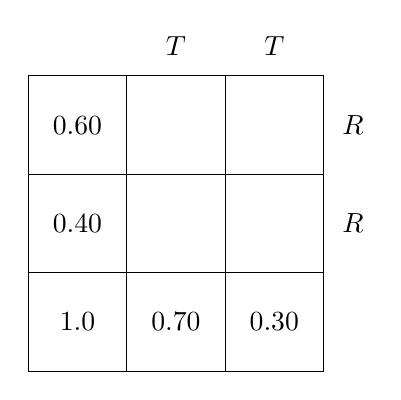
\begin{tikzpicture}[scale=1.25]
\draw (0,0) grid (3,3);
\node at (2.5,3.3) {$\bm{T}$};
\node at (1.5,3.3) {$\bover{T}$};
\node at (3.3,2.5) {$\bm{R}$};
\node at (3.3,1.5) {$\bover{R}$};
\node at (0.5,2.5) {$0.60$};
\node at (2.5,0.5) {$0.30$};
\node at (.5,.5) {$1.0$};
\node at (1.5,.5) {$0.70$};
\node at (.5,1.5) {$0.40$};
\end{tikzpicture}
\end{center}
שוב נסתמך על העובדה שהאירועים בלתי תלויים ונקבל:
\[
P(R\cap T)=P(R)\cdot P(T)=0.6\cdot 0.3=0.18\,,
\]
ואז יש לנו מספיק נתונים למלא את הטבלה:
\begin{center}
\selectlanguage{english}
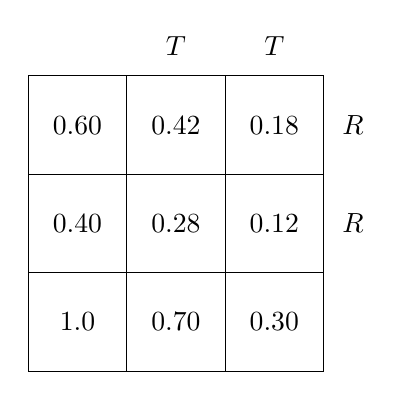
\begin{tikzpicture}[scale=1.25]
\draw (0,0) grid (3,3);
\node at (2.5,3.3) {$\bm{T}$};
\node at (1.5,3.3) {$\bover{T}$};
\node at (3.3,2.5) {$\bm{R}$};
\node at (3.3,1.5) {$\bover{R}$};
\node at (2.5,2.5) {$0.18$};
\node at (0.5,2.5) {$0.60$};
\node at (1.5,2.5) {$0.42$};
\node at (0.5,1.5) {$0.40$};
\node at (0.5,0.5) {$1.0$};
\node at (1.5,0.5) {$0.70$};
\node at (2.5,0.5) {$0.30$};
\node at (1.5,1.5) {$0.28$};
\node at (2.5,1.5) {$0.12$};
\end{tikzpicture}
\end{center}
סעיף א. חישבנו ש-%
$P(R\cap T)=0.18$.

סעיף ב. המילים "כל התושבים המשתתפים בחוג לריקודי עם,
\textbf{ורק הם}"
מכוונות להסתברות מותנית. אם ידוע שתושב משתתף בריקודי עם, ההסתברות שהוא משתתף גם בתאטרון היא:
\[
P(T/R) = \frac{P(T\cap R)}{P(R)}= \frac{0.18}{.060} = 0.3\,.
\]
כדי לחשב "לפחות שניים" עדיף לחשב את המשלים ל-"אפס או אחד":
\[
1-{6\choose 0}(0.3)^0(0.7)^6 -{6\choose 1}(0.3)^1(0.7)^5=0.5798\,.
\]

%%%%%%%%%%%%%%%%%%%%%%%%%%%%%%%%%%%%%%%%%%%%%%%%%%%%%%%%%%%%%%%%%%%
\newpage

\textbf{\R{
קיץ תשע"ד, מועד א
}}

\begin{center}
\selectlanguage{english}
\includegraphics[width=.9\textwidth]{summer-2014a-3}
\end{center}
\vspace{-2ex}
סעיף א. איור~%
\L{\ref{fig.winter-2014.2}}
)למעלה( מראה את צבירת הנקודות של 
\textbf{אבא}
בשני הסיבובים. המצבים בהם אבא צובר
\textbf{יותר}
מנקודה אחת מסומנים בכוכבית. ההסתברות של האירוע היא:
\[
0.2\cdot 0.2 \,+\, 0.2\cdot 0.7 \,+\, 0.7\cdot 0.2 \,=\,0.32\,.
\]
סעיף ב. איור~%
\L{\ref{fig.winter-2014.2}}
)למטה( מראה את צבירת הנקודות של
\textbf{דני}
בשני הסיבובים. המצבים בהם דני צובר 
\textbf{לפחות}
נקודה אחת מסומנים בכוכבית. ההסתברות של האירוע היא:
\[
0.2\cdot 0.1 \,+\,0.1\cdot 0.2 \,+\, 0.1\cdot 0.1 \,+\,0.1\cdot 0.7 \,+\, 0.7\cdot 0.1\,+\,0.7\cdot 0.7\,=\,0.68\,.
\]
סעיף ג. המילים
"\textbf{ידוע כי}"
מכוונות להסתברות מותנית והחיתוך מצטמצם כי אם יש תיקו אחד וניצחון של דני אז דני צבר לפחות נקודה אחת:
\vspace{-2ex}
\[
\renewcommand{\arraystretch}{2}
\begin{array}{c}
P(\textrm{\R{תיקו אחד, ניצחון אחד לדני}} / \textrm{\R{דני צבר לפחות נקודה אחת}})=\\
\displaystyle\frac{
P(\textrm{\R{תיקו אחד, ניצחון אחד לדני}} \cap \textrm{\R{דני צבר לפחות נקודה אחת}})
}
{P(\textrm{\R{דני צבר לפחות נקודה אחת}})}=\\
\displaystyle\frac{
P(\textrm{\R{תיקו אחד, ניצחון אחד לדני}})
}
{P(\textrm{\R{דני צבר לפחות נקודה אחת}})}\,.
\end{array}
\]
נחשב את המנה על ידי חיבור ההסתברויות של שני מסלולים בעץ המסומנים ב-%
$\#$:
\[
\frac{0.1\cdot 0.7 \,+\, 0.7\cdot 0.1}{0.68} = .2059\,.
\]
סעיף ד. בסעיף ב חישבנו את ההסתברות של האירוע בכל סיבוב, ונשאר רק לחשב:
\vspace{-1ex}
\[
{4\choose 2}(0.68)^2 (0.32)^2= 0.2841\,.
\]
\vspace{-2ex}
\begin{figure}[H]
\begin{center}
\selectlanguage{english}
\begin{tikzpicture}
[align=left,grow=right,
level 1/.append style={font=\sffamily,level distance=3cm,sibling distance=8em},
level 2/.append style={font=\sffamily,level distance=4cm,sibling distance=3em}]
\node at (-1,3) {$0.2=$ \R{אבא}\\%
$0.1=$ \R{דני}\\%
$0.7=$ \R{תיקו}};
\node[left] {$0$} % root
child {
  node[right] {$\frac{1}{2}$}
    child {
      node[right] {$1$}
      edge from parent node[below,yshift=-1mm] {$0.7$}
    }
    child {
      node[right] {$\frac{1}{2}$}
      edge from parent node[below,xshift=4mm] {$0.1$}
    }
    child {
      node[right] {$1\frac{1}{2}\quad *$}
      edge from parent node[above,yshift=1mm] {$0.2$}
    }
    edge from parent node[below,yshift=-3mm] {$0.7$}
}
child {
  node[right] {$0$}
    child {
      node[right] {$\frac{1}{2}$}
      edge from parent node[below,yshift=-1mm] {$0.7$}
    }
    child {
      node[right] {$0$}
      edge from parent node[below,xshift=4mm] {$0.1$}
    }
    child {
      node[right] {$1$}
      edge from parent node[above,yshift=1mm] {$0.2$}
    }
    edge from parent node[below] {$0.1$}
}
child {
  node[right] {$1$}
    child {
      node[right] {$1\frac{1}{2}\quad *$}
      edge from parent node[below,yshift=-1mm] {$0.7$}
    }
    child {
      node[right] {$1$}
      edge from parent node[below,xshift=4mm] {$0.1$}
    }
    child {
      node[right] {$2\quad *$}
      edge from parent node[above,yshift=1mm] {$0.2$}
    }
    edge from parent node[above,yshift=3mm] {$0.2$}
};
\end{tikzpicture}
%\selectlanguage{hebrew}
%\caption{עץ ההסתברויות של המשחקים: צבירת נקודות של אבא}\label{fig.winter-2014.1}
%\end{center}
%\end{figure}
%
%
%\begin{figure}[H]
%\begin{center}
%\selectlanguage{english}
\bigskip

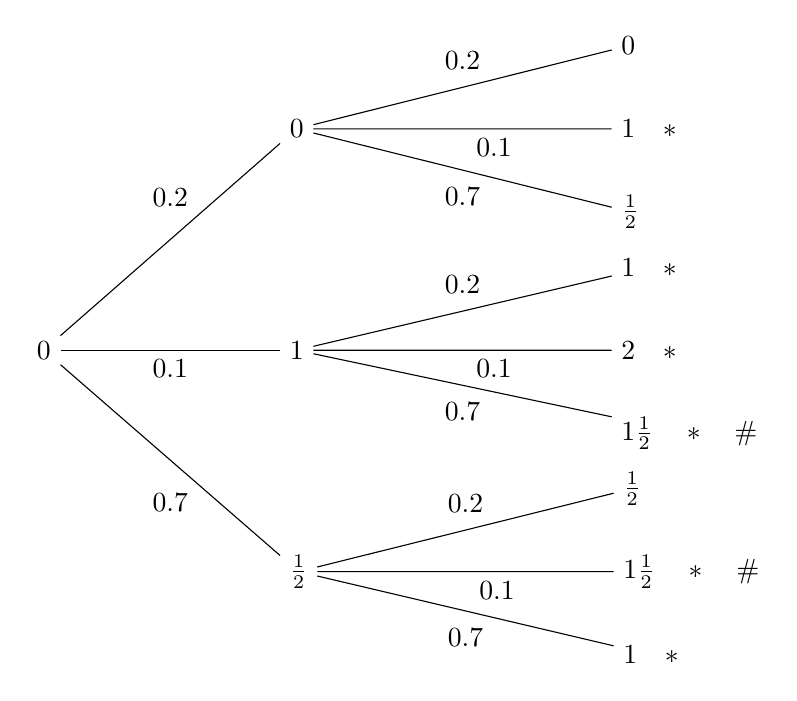
\begin{tikzpicture}
[grow=right,
level 1/.append style={font=\sffamily,level distance=3cm,sibling distance=8em},
level 2/.append style={font=\sffamily,level distance=4cm,sibling distance=3em}]
\node[left] {$0$} % root
child {
  node[right] {$\frac{1}{2}$}
    child {
      node[right] {$1\quad *$}
      edge from parent node[below,yshift=-1mm] {$0.7$}
    }
    child {
      node[right] {$1\frac{1}{2}\quad *\quad \#$}
      edge from parent node[below,xshift=4mm] {$0.1$}
    }
    child {
      node[right] {$\frac{1}{2}$}
      edge from parent node[above,yshift=1mm] {$0.2$}
    }
    edge from parent node[below,yshift=-3mm] {$0.7$}
}
child {
  node[right] {$1$}
    child {
      node[right] {$1\frac{1}{2}\quad *\quad \#$}
      edge from parent node[below,yshift=-1mm] {$0.7$}
    }
    child {
      node[right] {$2\quad *$}
      edge from parent node[below,xshift=4mm] {$0.1$}
    }
    child {
      node[right] {$1\quad *$}
      edge from parent node[above,yshift=1mm] {$0.2$}
    }
    edge from parent node[below] {$0.1$}
}
child {
  node[right] {$0$}
    child {
      node[right] {$\frac{1}{2}$}
      edge from parent node[below,yshift=-1mm] {$0.7$}
    }
    child {
      node[right] {$1\quad *$}
      edge from parent node[below,xshift=4mm] {$0.1$}
    }
    child {
      node[right] {$0$}
      edge from parent node[above,yshift=1mm] {$0.2$}
    }
    edge from parent node[above,yshift=3mm] {$0.2$}
};
\end{tikzpicture}
\selectlanguage{hebrew}
\setlength{\belowcaptionskip}{-4ex}
\caption{עץ ההסתברויות של צבירת נקודות של אבא )למעלה( ודני )למטה(}\label{fig.winter-2014.2}
\end{center}
\end{figure}


%%%%%%%%%%%%%%%%%%%%%%%%%%%%%%%%%%%%%%%%%%%%%%%%%%%%%%%%%%%%%%%%%%%

\textbf{\R{
קיץ תשע"ד, מועד ב
}}

\begin{center}
\selectlanguage{english}
\includegraphics[width=.95\textwidth]{summer-2014b-3}
\end{center}

נמלא את הטבלה ממידע הנתון. נתון ש-% 
$0.4$
מהתלמידים הן בנות. 
$10\%$
מהם בחרו במסלול ב, ולכן נרשום
$0.1\times 0.4=.04$
מעל לתא עם הנתון הראשון. הסתברות המשלימה היא
$0.4-0.04=0.36$.
נתון ש-%
$75\%$
מהתלמידים שבחרו במסלול א הן בנות:
$0.75 \cdot \aleph = 0.36$,
ולכן 
$0.48$
מהתלמידים בחרו מסלול א. ניתן למלא את שאר התאים בטבלה לפי ההסתברויות המשלימות:
\begin{center}
\selectlanguage{english}
\begin{tikzpicture}[scale=2.2]
\draw (0,0) grid (3,3);
\node at (2.5,3.3) {\sffamily\bfseries \R{בנות}};
\node at (1.5,3.3) {\sffamily\bfseries \R{בנים}};
\node at (3.3,2.5) {\sffamily\bfseries \R{א}};
\node at (3.3,1.5) {\sffamily\bfseries \R{ב}};
\node at (2.5,2.7) {$.4-.04=$};
\node at (2.5,2.3) {$.36$};
\node at (0.5,2.7) {$.36/.75=$};
\node at (0.5,2.3) {$.48$};
\node at (1.5,2.7) {$.48-.36=$};
\node at (1.5,2.3) {$.12$};
\node at (0.5,1.7) {$1-.48=$};
\node at (0.5,1.3) {$.52$};
\node at (0.5,0.5) {$1$};
\node at (1.5,0.7) {$1-.4=$};
\node at (1.5,0.3) {$.6$};
\node at (2.5,0.7) {\sffamily\bfseries \R{נתון}};
\node at (2.5,0.3) {$0.4$};
\node at (1.5,1.7) {$.52-.04=$};
\node at (1.5,1.3) {$.48$};
\node at (2.5,1.7) {$.1\times .4=$};
\node at (2.5,1.3) {$.04$};
\end{tikzpicture}
\end{center}
בצורה יותר מפורשת תוך שימוש בהסתברות מותנית:
\[
0.1 = P(\textrm{\R{מסלול ב}} / \textrm{\R{בנות}})=
\displaystyle\frac{
P(\textrm{\R{מסלול ב}} \cap \textrm{\R{בנות}})
}
{P(\textrm{\R{בנות}})}=
\displaystyle\frac{
P(\textrm{\R{מסלול ב}} \cap \textrm{\R{בנות}})
}
{0.4}\,.
\]
מכאן ש:
\[
P(\textrm{\R{מסלול ב}} \cap \textrm{\R{בנות}})
=0.4\cdot 0.1= 0.04\,.
\]
לפי הסתברות משלימה:
\[
P(\textrm{\R{מסלול א}} \cap \textrm{\R{בנות}}) 
= 0.40-0.04=0.36\,.
\]
נמשיך עם הנתון הנוסף:
\[
0.75 = P(\textrm{\R{בנות}} / \textrm{\R{מסלול א}})=
\displaystyle\frac{
P(\textrm{\R{בנות}} \cap \textrm{\R{מסלול א}})
}{P(\textrm{\R{מסלול א}})}=\frac{0.36}{P(\textrm{\R{מסלול א}})}\,.
\]
מכאן ש:
\[
P(\textrm{\R{מסלול א}})=\frac{0.36}{0.75}=0.48\,.
\]
סעיף א. הסעיף מבקש
$P(\textrm{\R{מסלול א}})$
וחישבנו שערכו 
$0.48$.
לכאורה, נראה שמדובר בהסתברות מותנית, אבל מה שידוע הוא שבחרנו 
\textbf{תלמיד כלשהו},
וההסתברות היא אחת.

סעיף ב.
\begin{eqnarray*}
P(\textrm{\R{התלמיד הוא בת}} \cap \textrm{\R{מסלול א}}) &=& 
0.36\\
P(\textrm{\R{התלמיד הוא בת}}) \cdot P(\textrm{\R{מסלול א}})
&=&0.4 \cdot 0.48 = 0.192\,.
\end{eqnarray*}
האירועים
\textbf{אינם}
בלתי תלויים.

סעיף ג. כדי לחשב
"\textbf{לפחות אחת}",
נחשב שת ההסתברות המשלימה ל-%
"\textbf{אף אחת}".
ההסתברות שבת לא תבחר מסלול א היא ההסתברות שהיא תבחר מסלול ב:
\[
P(\textrm{\R{מסלול ב}} / \textrm{\R{בת}})=
\displaystyle\frac{
P(\textrm{\R{מסלול ב}} \cap \textrm{\R{בת}})
}{P(\textrm{\R{בת}})}
=\frac{0.04}{0.4}=0.1\,.
\]
נפתור את המשוואה:
\[
(0.1)^n=1-0.99=0.01\,,
\]
ונקבל 
$n=2$.
%%%%%%%%%%%%%%%%%%%%%%%%%%%%%%%%%%%%%%%%%%%%%%%%%%%%%%%%%%%%%%%%%%%

\newpage

\begin{center}
\textbf{סיכום}
\end{center}

\begin{itemize}
\item
\textbf{קרא בזהירות את השאלה}. 
לעתים השאלות ארוכות )בחינות של קיץ תשע"ה א, קיץ תשע"ח ב( וחשוב להבין את המשמעות של כל פסקה.

%%%%%%%%%%%%%%%%%%%%%%%%%%%%%%%%%%%%

\item
כמעט כל הבחינות מכילות שאלות על 
\textbf{הסתברות מותנית}.
ניסוחים רבים מכוונים להסתברות מותנית וחשוב להכיר אותם!

\begin{itemize}
\item
הניסוח השכיח ביותר משתמש במילים
"\textbf{אם ידוע ש-}"
או
"\textbf{ידוע כי}".

\item
בבחינה של חורף תשע"ז
כתוב "%
\textbf{אם} $\ldots$ ,
\textbf{מהי ההסתברות} $\ldots$".
לא לגמרי ברור שלמילה "אם" יש משמעות של "אם ידוע", אבל זאת הכוונה.

\item
לעתים קרובות )למשל, בבחינה של קיץ תשע"ה ב( כתוב "%
\textbf{מה ההסתברות לבחור} $\ldots$
\textbf{מבין} $\ldots$".

\item
יוצא מן הכלל: בבחינה של קיץ תשע"ו א כתוב
"\textbf{מבין}
כל הנבחנים" והמילה "מבין" בדרך כלל מכוונת להסתברות מותנית, אבל כאשר "מבין" מתייחס ל-%
"\textbf{כל}
הנבחנים" אין הסתברות מותנית, או ההסתברות מותנית בהסתברות שהיא 
$1$,
והחיתוך מצטמצם:
\[
P(X/\textrm{\R{כל הנבחנים}})=
\frac{P(X\cap \textrm{\R{כל הנבחנים}})}
{P(\textrm{\R{כל הנבחנים}})} = 
\frac{P(X)}{1}=P(X)\,.
\]
מצב דומה מופיע בבחינה של קיץ תשע"ד ב )"בוחרים באקראי תלמיד י"ב )בן/בת("(, ובבחינה של קיץ תשע"ח ב )"מן התלמידים שנגשו למבחן"(.

\item
בבחינה של קיץ תשע"ח א הניסוח הוא: "%
$\ldots X\%$
נעזרו 
$\ldots$.
$\displaystyle\frac{k}{n}$
\textbf{מהם}
עברו את הבחינה".

\item
בבחינה של חורף תשע"ד יש ניסוח אחר:
\textbf{כל התושבים המשתתפים ב-} $\ldots$,
\textbf{ורק הם}.
\end{itemize}

%%%%%%%%%%%%%%%%%%%%%%%%%%%%%%%%%%%%

\item
כאשר יש חיתוך בחישוב של הסתברות מותנית, לעתים קרובות ניתן לפשט את החישוב. בבחינה של קיץ תשע"ז א יש לחשב
$P(D=4\cap D\ge 3)$,
אבל אם ערך גדול או שווה
$3$
\textbf{וגם}
שווה ל-%
$4$,
אז הוא שווה ל-%
$4$, 
ולכן מספיק לחשב
$P(D=4)$.

%%%%%%%%%%%%%%%%%%%%%%%%%%%%%%%%%%%%

\item
כאשר יש חיתוך בין שני אירועים בלתי תלויים, חישוב ההסתברות המותנית מצטמצם )בחינה של קיץ תשע"ה א(:
\[
\renewcommand{\arraystretch}{2.4}
\begin{array}{l}
\displaystyle\frac{
P(\textrm{\R{סכום זוגי}} \cap \textrm{\R{ספרה ראשונה זוגית}})
}{P(\textrm{\R{ספרה ראשונה זוגית}})}=\\
\displaystyle\frac{
P(\textrm{\R{סכום זוגי}}) \cdot P(\textrm{\R{ספרה ראשונה זוגית}})
}
{P(\textrm{\R{ספרה ראשונה זוגית}})}=\\
P(\textrm{\R{סכום זוגי}})
\,.
\end{array}
\]
מצב דומה מופיע בבחינות של חורף תשע"ז וחורף משע"ח.
%%%%%%%%%%%%%%%%%%%%%%%%%%%%%%%%%%%%

\item
בבחינה של חורף תשע"ד נתון
$P(T/R)$
וגם נתון ששני אירועים הם
\textbf{בלתי תלויים}.
החיתוך שווה למכפלת ההסתברויות והחישוב מצטמצם:
\[
P(T/R) = \frac{P(T \cap R)}{P(R)} =\frac{P(T)\cdot P(R)}{P(R)} = P(T)\,.
\]
\vspace{-4ex}
%%%%%%%%%%%%%%%%%%%%%%%%%%%%%%%%%%%%

\item
המילה 
\textbf{בדיוק}
מכוונת לחישוב אחד של נוסחת ברנולי, כי נתון כמה "הצלחות" צריכות להיות וגם כמה "כשלונות". מקרה מעניין נמצא בבחינה של קיץ תשע"ח ב כאשר נתון שההסתברות לקבל 
$60$
שווה להסתברות לקבל
$100$.
נתון גם שיש שלוש הצלחות מתוך חמש )%
$20$
נקודות כל אחת(, אז ההסתברות לקבל שני כשלונות )%
$20$
נקודות כל אחת( צריכה להיות שווה להסתברות לקבל שתי הצלחות )%
$20$
נקודות כל אחת(.

%%%%%%%%%%%%%%%%%%%%%%%%%%%%%%%%%%%%

\item
בבחינה של קיץ תשע"ז א כתוב "%
\textbf{בוחרים באקראי}
$\ldots$,
\textbf{עד של-}
$3$
מהם
\textbf{בדיוק}
יש קלנועית". המשמעות של "עד ש-" היא שמפסיקים את הבחירה האקראית כאשר הבחירה 
\textbf{האחרונה} 
היא "הצלחה". במקרה זה נשארו שתי "הצלחות" שיש לחשב את ההסתברות שלהן לפי נוסחת ברנולי, ואז להכפיל בהסתברות של "הצלחה" בבחירה האחרונה:
\[
\overbrace{\pm\;\pm\;\pm\;\pm\;\pm}^{2/5}\quad\quad \overbrace{+}^{1/1}\,.
\]
\vspace{-6ex}
%%%%%%%%%%%%%%%%%%%%%%%%%%%%%%%%%%%%

\item
בבחינה של קיץ תשע"ז ב הביטוי "מוציאים באקראי
$\ldots$",
ובהמשך הביטוי "מוציאים באקראי
\textbf{שוב}
$\ldots$"
מכוון לשימוש בעץ כדי לתאר את הבחירה הסדרתית.

%%%%%%%%%%%%%%%%%%%%%%%%%%%%%%%%%%%%

\item
בבחינה של קיץ תשע"ח א, המשמעות של הניסוח "%
\textbf{לפחות אחת}
משתי הטענות 
$I, II$"
היא שהאירוע קורה אם קורה אחד מהאירועים
$I, II$,
\textbf{או שניהם},
המסומן 
$I \cup II$.
יש שתי דרכים לחשב את ההסתברות: על ידי חיבור ההסתברות של שני האירועים וחיסור האירוע המשותף כדי לקזז את הספירה הכפולה, או לחבר את האירוע המשותף עם האירועים של אחד ולא השני המסומן 
$I-II, II-I$:
\begin{eqnarray*}
P(I \cup II) &=& P(I) + P(II) - P(I \cap II)\\
P(I \cup II) &=& P(I-II) + P(II-I) + P(I \cap II)\,.
\end{eqnarray*}
הערכים לחישוב
$P(I \cup II)$
בשתי הדרכים מסומנים בטבלה להלן, כאשר התא המקווקו מופיע פעמיים, פעם כחלק מהאירוע
$I$
ופעם כחלק מהאירוע
$II$:
\begin{center}
\selectlanguage{english}
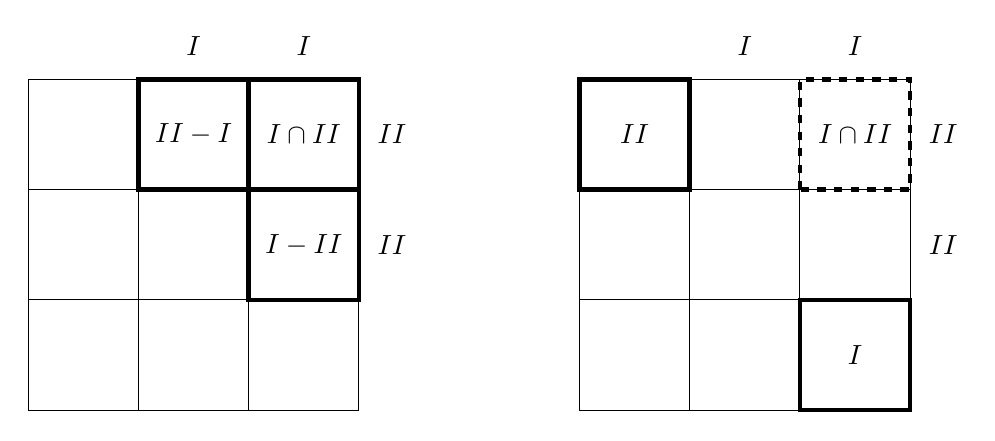
\begin{tikzpicture}[scale=1.4]
\begin{scope}
\draw (0,0) grid (3,3);
\node at (2.5,3.3) {$\bm{I}$};
\node at (1.5,3.3) {$\bover{I}$};
\node at (3.3,2.5) {$\bm{II}$};
\node at (3.3,1.5) {$\bover{II}$};
\node at (2.5,2.5) {$I\cap II$};
\node at (2.5,1.5) {$I-II$};
\node at (1.5,2.5) {$II-I$};
\draw[ultra thick] (2,2) rectangle +(1,1);
\draw[ultra thick] (1,2) rectangle +(1,1);
\draw[ultra thick] (2,1) rectangle +(1,1);
\end{scope}
\begin{scope}[xshift=5cm]
\draw (0,0) grid (3,3);
\node at (2.5,3.3) {$\bm{I}$};
\node at (1.5,3.3) {$\bover{I}$};
\node at (3.3,2.5) {$\bm{II}$};
\node at (3.3,1.5) {$\bover{II}$};
\node at (2.5,2.5) {$I\cap II$};
\node at (2.5,0.5) {$I$};
\node at (0.5,2.5) {$II$};
\draw[ultra thick] (0,2) rectangle +(1,1);
\draw[ultra thick] (2,0) rectangle +(1,1);
\draw[ultra thick,dashed] (2,2) rectangle +(1,1);
\end{scope}
\end{tikzpicture}
\end{center}

%%%%%%%%%%%%%%%%%%%%%%%%%%%%%%%%%%%%

\item
בבחינה של חורף תשע"ו נתון ההסתברות
$p$
ש-"לא יזכה
\textbf{באף משחק}
מתוך 
$n$
משחקים". גם בבחינה של  קיץ תשע"ח ב צריכים לחשב את ההסבתרות של תשובה נכונה 
\textbf{לכל}
השאלות או תשובה נכונה
\textbf{לאף אחת}
מהשאלות.  אין צורך להשתמש בנוסחת ברנולי במלואו:
\[
{n \choose k}p^k(1-p)^{n-k}\,.
\]
אם
$k=0$
או
$k=n$,
${n\choose k}=1$.
גם
$p^n(1-p)^0=p^n\cdot 1$
או
$p^0(1-p)^n=1\cdot(1-p)^n$,
ונשאר רק גורם אחד 
$p^n$
או
$(1-p)^n$.

%%%%%%%%%%%%%%%%%%%%%%%%%%%%%%%%%%%%

\item
בבחינות של קיץ תשע"ו א, ב יש שלוש תוצאות אפשרויות במקום שתיים. סכום ההסתברויות חייב להיות אחד, ולכן כאשר מחשבים משלים להסתברות אחת, יש להחסיר את שתי ההסתברויות האחרות. בבחינה של מועד ב, ההסתברות לתיקו היא אחד פחות ההסתברות שיעל תנצח פחות ההסתברות אנה תנצח:
\[
P(\textrm{\R{תיקו}}) =
1 - (P(\textrm{\R{יעל}})+
P(\textrm{\R{אנה}})) = 
1 - P(\textrm{\R{יעל}})-
P(\textrm{\R{אנה}}) \,.
\]
\vspace{-4ex}
\item 
במספר בחינות )חורף תשע"ה, קיץ תשע"ד ב, קיץ תשע"ה ב( כתוב "ישוב גדול", "עיר גדולה", "אוניברסיטה גדולה". אני מניח שבמילה "גדול" מבטיחה שאפשר לבחור תושבים או סטודנטים כפי שדרוש  בשאלות. אין משמעות לבחור ארבעה סטודנטים אם יש רק שניים באוניברסיטה.
\end{itemize}

\end{document}


\tikzsetfigurename{geometry}
\documentclass[12pt,a4paper]{article}
\usepackage[utf8x]{inputenc}
\usepackage[english,hebrew]{babel}
\usepackage{graphicx}
\usepackage{verbatim}
\usepackage{url}
\usepackage{bm}
\usepackage{float}

\graphicspath{{images/}}

\usepackage{tikz}
\usetikzlibrary{positioning,through,calc,intersections,arrows.meta}
\usepackage{tkz-euclide}
\usetkzobj{all}

%\usetikzlibrary{external}
%\tikzexternalize[prefix=tikz/]

% Use stealth arrows
\tikzset {
  >=stealth
}

\textwidth=15.5cm
\textheight=23cm
\topmargin=0pt
\headheight=0pt
\oddsidemargin=2em
\headsep=0pt
\parindent=0pt
\renewcommand{\baselinestretch}{1.1}
\setlength{\parskip}{0.3\baselineskip plus 1pt minus 1pt}

\newcommand{\bover}[1]{\bm{\overline{#1}}}

\begin{document}
\thispagestyle{empty}

\selectlanguage{hebrew}

%\begin{comment}

\begin{center}
\textbf{\Huge גיאומטריה}

\bigskip
\bigskip
\bigskip

\textbf{\Large מוטי בן-ארי}

\bigskip

\textbf{\Large מכון ויצמן למדע}

\bigskip

\url{http://www.weizmann.ac.il/sci-tea/benari/}

\bigskip

\end{center}

\selectlanguage{english}

\vfill

\begin{center}
\sffamily\copyright{}\  2018 by Moti Ben-Ari.
\end{center}

\begin{footnotesize}
\sffamily
This work is licensed under the Creative Commons Attribution-ShareAlike 3.0 Unported License. To view a copy of this license, visit \url{http://creativecommons.org/licenses/by-sa/3.0/} or send a letter to Creative Commons, 444 Castro Street, Suite 900, Mountain View, California, 94041, USA.
\end{footnotesize}

\begin{center}
\includegraphics[width=.2\textwidth]{../../by-sa.png}
\end{center}

\newpage
\selectlanguage{hebrew}


במסמך זה אביא פתרונות לשאלות על גיאומטריה )שאלה 4( בבחינות הבגרות )שאלון
$806$(.
אנסה לתאר את דרכי החשיבה המובילות לפתרונות עם דגש על בחירת המשפטים שמשתמשים בהם בפתרונות, תוך ציון מספרי המשפטים כפי שמופיע ברשימה של משרד החינוך. בסוף אביא מספר המלצות המבוססות על תהליכי הפתרון.

%\end{comment}

%%%%%%%%%%%%%%%%%%%%%%%%%%%%%%%%%%%%%%%%%%%%%%%%%%%%%%%%%%%%%%%%%%%

%\begin{comment}

\section*{קיץ תשע"ח מועד ב}

\begin{center}
\selectlanguage{english}
\includegraphics[width=\textwidth]{summer-2018b-4}
\end{center}
\vspace{-8mm}
\textbf{סעיף א}

%%%%%%%%%%%%%%%%%%%%%%%%%%%%%%%%%%%%%%%%%%%%%%%%%%%%%%%%%%%%%%%%%%%

\section*{קיץ תשע"ח מועד א}

\begin{center}
\selectlanguage{english}
\includegraphics[width=\textwidth]{summer-2018a-4}
\end{center}
\vspace{-8mm}
\textbf{סעיף א}
%\end{comment}

%%%%%%%%%%%%%%%%%%%%%%%%%%%%%%%%%%%%%%%%%%%%%%%%%%%%%%%%%%%%%%%%%%%

\section*{חורף תשע"ח}

\begin{center}
\selectlanguage{english}
\includegraphics[width=\textwidth]{winter-2018-4}
\end{center}
\vspace{-8mm}
\textbf{סעיף א}


%\begin{comment}

%%%%%%%%%%%%%%%%%%%%%%%%%%%%%%%%%%%%%%%%%%%%%%%%%%%%%%%%%%%%%%%%%%%

\section*{קיץ תשע"ז מועד ב}

\begin{center}
\selectlanguage{english}
\includegraphics[width=\textwidth]{summer-2017b-4}
\end{center}
\vspace{-8mm}
\textbf{סעיף א}

תהי 
$GF$
מקביל ל-%
$BC$
ו-%
$EH$
מקביל ל-%
$CD$.
לפי זוויות מתאימות ומשלימות, המרובעים 
$BEHG,ECFH$
הם מקביליות. בגלל ש-%
$E$
היא נקודת האמצע של
$BC$,
$H$
הוא נקודת האמצע של
$GF=BC$.
מכאן שהמשולשים 
$\triangle ECF,\triangle EHF$
חופפים, ו-%
$S_{EHF}=S_{ECF}=S$.
באותה דרך נוכיח ש-%
$S_{BEH}=S_{BGH}=S$,
ולכן
$S_{BCFG}=4S$.
$GF$
הוא קו אמצעים ומחלק את המקבילית לשני חלקים ששטחם שווה, כך ש-%
$S_{ABCD}=S_{BCFG}+S_{GFDA}=8S$.

\begin{center}
\selectlanguage{english}
\begin{tikzpicture}[scale=1]
\coordinate (B) at (0,0);
\coordinate (E) at (4,0);
\coordinate (C) at (8,0);
\draw[thick] (B) -- (C);
\draw[thick] (E) -- +(-30:4) coordinate (F);
\draw[thick] (C) -- ($(C) ! 2 ! (F)$) coordinate (D);
\draw[thick] (D) -- +(-8,0) coordinate (A) -- (B);
\fill (A) node[below left] {$A$} circle(1.5pt);
\fill (B) node[above left] {$B$} circle(1.5pt);
\fill (C) node[above right] {$C$} circle(1.5pt);
\fill (D) node[below right] {$D$} circle(1.5pt);
\fill (E) node[above] {$E$} circle(1.5pt);
\fill (F) node[right] {$F$} circle(1.5pt);
\coordinate (G) at ($(A)!.5!(B)$);
\fill (G) node[left] {$G$} circle(1.5pt);
\draw[thick,dashed] (G) -- (F);
\coordinate (H) at ($(G)!.5!(F)$);
\fill (H) node[below] {$H$} circle(1.5pt);
\draw[thick,dashed] (E) -- (H);
\end{tikzpicture}
\end{center}
\textbf{הוכחה אחרת}
לפי משפט
$5$%
א "שטח מקבילית שווה למכפלת צלע המקבילית בגובה לצלע זו". הגובה של המקבילית כפול מהגובה של המשולש לפי דמיון של משולשים 
$\triangle FCK, \triangle DCJ$.
חישוב השטחים נותן:
\begin{eqnarray*}
S_{ECF}&=&\frac{1}{2}ah=S\\
S_{ABCD}&=&2a\cdot 2h=4ah=8S\,.
\end{eqnarray*}
\begin{center}
\selectlanguage{english}
\begin{tikzpicture}[scale=1]
\coordinate (B) at (0,0);
\coordinate (E) at (4,0);
\coordinate (C) at (8,0);
\draw[thick] (B) -- (C);
\draw[thick] (E) -- +(-30:4) coordinate (F);
\draw[thick] (C) -- ($(C) ! 2 ! (F)$) coordinate (D);
\draw[thick] (D) -- +(-8,0) coordinate (A) -- (B);
\fill (A) node[below left] {$A$} circle(1.5pt);
\fill (B) node[above left] {$B$} circle(1.5pt);
\fill (C) node[above right] {$C$} circle(1.5pt);
\fill (D) node[below right] {$D$} circle(1.5pt);
\fill (E) node[above] {$E$} circle(1.5pt);
\fill (F) node[below left] {$F$} circle(1.5pt);
\draw[thick,dashed,name path=dj] (D) -- +(2.5,0);
\draw[thick,dashed,name path=cj] (C) -- ($(A)!(C)!(D)$);
\path[name intersections={of=dj and cj,by={J}}];
\fill (J) node[below] {$J$} circle(1.5pt);
\draw (J) rectangle +(7pt,7pt);
\coordinate (K) at ($(C)!.5!(J)$);
\fill (K) node[right] {$K$} circle(1.5pt);
\path (E) -- node[above] {$a$} (C);
\path (A) -- node[below] {$2a$} (D);
\draw[thick,dashed] (F) -- (K);
\draw[<->] ($(C)+(.8,0)$) -- node[fill=white] {$h$} ($(K)+(.8,0)$);
\draw[<->] ($(C)+(1.2,0)$) -- node[fill=white] {$2h$} ($(J)+(1.2,0)$);
\end{tikzpicture}
\end{center}
\textbf{סעיף ב}
הדרך לחפש יחס בין קטעי קו היא למצוא משולשים דומים שקטעי הקו הם צלעות של המשולשים. קצת קשה לראות אותם אלא אם נפשט את הציור. קטע האמצעים במקבילית מקביל לבסיסים,
$BC\|GF$,
ומזוויות מתחלפות אנו מקבלים ש-%
$\triangle LMB \sim \triangle KMF$.
מתכונות המקבילית רשמנו את אורכי הקטעים תוך שימוש בנעלמים
$a,b,c$.

\begin{center}
\selectlanguage{english}
\begin{tikzpicture}[scale=1]
\coordinate (B) at (0,0);
\coordinate (E) at (4,0);
\coordinate (C) at (8,0);
\draw[thick] (B) -- (C);
\path (E) -- +(-30:4) coordinate (F);
\draw[thick] (C) -- ($(C) ! 2 ! (F)$) coordinate (D);
\draw[thick] (D) -- +(-8,0) coordinate (A) -- (B);
\draw[thick,name path=bf] (B) -- (F);
\fill (A) node[below left] {$A$} circle(1.5pt);
\fill (B) node[above left] {$B$} circle(1.5pt);
\fill (C) node[above right] {$C$} circle(1.5pt);
\fill (D) node[below right] {$D$} circle(1.5pt);
\fill (E) node[above] {$E$} circle(1.5pt);
\fill (F) node[right] {$F$} circle(1.5pt);
\coordinate (G) at ($(A)!.5!(B)$);
\fill (G) node[left] {$G$} circle(1.5pt);
\draw[thick,dashed,name path=gf] (G) -- (F);
\coordinate (L) at (2,0);
\draw[thick,dashed,name path=ln] (L) -- ($(A)!.25!(D)$) coordinate (N);
\fill (L) node[above] {$L$} circle(1.5pt);
\fill (N) node[below] {$N$} circle(1.5pt);
\path[name intersections={of=bf and ln,by={M}}];
\fill (M) node[below left] {$M$} circle(1.5pt);
\path[name intersections={of=gf and ln,by={K}}];
\fill (K) node[below left ] {$K$} circle(1.5pt);
\draw[thick] (L) -- (K);
\draw[thick] (K) -- (F);
\path (B) -- node[above] {$a$} (L);
\path (B) -- node[left] {$b$} (G);
\path (G) -- node[left] {$b$} (A);
\path (K) -- node[left] {$b$} (N);
\path (K) -- node[below] {$3a$} (F);
\path (L) -- node[right] {$c$} (M);
\path (M) -- node[left] {$b-c$} (K);
\end{tikzpicture}
\end{center}
\vspace{-3ex}
\begin{eqnarray*}
\frac{c}{b-c}&=&\frac{a}{3a}=\frac{1}{3}\\
b&=&4c\\
\frac{LM}{MN}&=&\frac{c}{2b-c}\\
&=&\frac{a}{2\cdot 4c-c}\\
&=&\frac{1}{7}\,.
\end{eqnarray*}

\textbf{סעיף ג}
לפי משפט
$72$
"במעגל, כל הזוויות ההיקפיות הנשענות על מיתר מאותו צד של המיתר שוות זו לזו" ומשפט
$73$
"זווית היקפית הנשענת על קוטר היא זווית ישרה", 
$\angle BFC=90^\circ$.
נסמן
$\angle CBF=\alpha$
ונשלים את הסימונים בציור כאשר אנו יודעים ש-%
$\triangle BEF,\triangle CEF$
שווה שוקיים, והזוויות הנגדיות במקבילית שוות. לפי משפט
$56$
"ניתן לחסום מרובע במעגל אם ורק אם סכום זוג זוויות נגדיות שווה ל-%
$180^\circ$".
אבל
$(90-\alpha)+90=180-\alpha=180$,
וזה לא ייתכן אלא אם
$\alpha=0$.
אבל לא ייתכן כי נתון ש-%
$\alpha$
היא זווית חדה. )בהגדרת זווית חדה יש לציין שהיא חייבת להיות גדול מאפס.(
\begin{center}
\selectlanguage{english}
\begin{tikzpicture}[scale=1]
\coordinate (B) at (0,0);
\coordinate (E) at (4,0);
\coordinate (C) at (8,0);
\draw[thick] (B) -- (C);
\draw[thick] (E) -- +(-30:4) coordinate (F);
\draw[thick] (C) -- ($(C) ! 2 ! (F)$) coordinate (D);
\draw[thick] (D) -- +(-8,0) coordinate (A) -- (B);
\draw[thick,name path=bf] (B) -- (F);
\fill (A) node[below left] {$A$} circle(1.5pt);
\fill (B) node[above left] {$B$} circle(1.5pt);
\fill (C) node[above right] {$C$} circle(1.5pt);
\fill (D) node[below right] {$D$} circle(1.5pt);
\fill (E) node[above] {$E$} circle(1.5pt);
\fill (F) node[right] {$F$} circle(1.5pt);
\path (B) -- node[above] {$a$} (E) -- node[above] {$a$} (C);
\path (E) -- node[above] {$a$} (F);
\draw[rotate=75] (F) rectangle +(7pt,7pt);
\node[below right,xshift=28pt,yshift=2pt] at (B) {$\alpha$};
\node[above left,xshift=-28pt,yshift=8pt] at (F) {$\alpha$};
\node[below left,xshift=0pt,yshift=2pt] at (C) {$90-\alpha$};
\node[above right,xshift=6pt,yshift=2pt] at (A) {$90-\alpha$};
\node[below left,xshift=-6pt,yshift=2pt] at (F) {$90$};
\end{tikzpicture}
\end{center}
יש לי בעיה עם השימוש כאן במשפט
$72$,
כי הוא לא מנוסח כ-"אם ורק אם". לא קשה להוכיח את הכיוון ההפוך כי כל הנקודות הנמצאות במרחק שווה מנקודה 
$E$
נמצאות על מעגל שמרכזו 
$E$.

אפשר להגיע לאותה משוואה
$180-\alpha=180$,
ללא שימוש במשפט
$72$,
אלא רק בעובדות ש: )א( המרובע
$ABCD$
הוא מקבילית, )ב( המשולשים 
$\triangle BEF,\triangle CEF$
שווה שוקיים, )ג( זוויות משלימות ב-%
$E,F$:
\begin{center}
\selectlanguage{english}
\begin{tikzpicture}[scale=1]
\coordinate (B) at (0,0);
\coordinate (E) at (4,0);
\coordinate (C) at (8,0);
\draw[thick] (B) -- (C);
\draw[thick] (E) -- +(-30:4) coordinate (F);
\draw[thick] (C) -- ($(C) ! 2 ! (F)$) coordinate (D);
\draw[thick] (D) -- +(-8,0) coordinate (A) -- (B);
\draw[thick,name path=bf] (B) -- (F);
\fill (A) node[below left] {$A$} circle(1.5pt);
\fill (B) node[above left] {$B$} circle(1.5pt);
\fill (C) node[above right] {$C$} circle(1.5pt);
\fill (D) node[below right] {$D$} circle(1.5pt);
\fill (E) node[above] {$E$} circle(1.5pt);
\fill (F) node[right] {$F$} circle(1.5pt);
\path (B) -- node[above] {$a$} (E) -- node[above] {$a$} (C);
\path (E) -- node[above] {$a$} (F);
%\draw[rotate=75] (F) rectangle +(7pt,7pt);
\node[below right,xshift=28pt,yshift=2pt] at (B) {$\alpha$};
\node[above left,xshift=-28pt,yshift=8pt] at (F) {$\alpha$};
\node[below left,xshift=0pt,yshift=2pt] at (C) {$90-\alpha$};
\node[above right,xshift=6pt,yshift=2pt] at (A) {$90-\alpha$};
\node[below left,xshift=-6pt,yshift=2pt] at (F) {$90$};
\node[above,xshift=40pt,yshift=2pt] at (F) {$90-\alpha$};
\node[below left,xshift=4pt,yshift=2pt] at (E) {$180-2\alpha$};
\node[below right,xshift=16pt,yshift=2pt] at (E) {$2\alpha$};
\draw[->] ($(F)+(20pt,10pt)$) -- +(-25pt,0);
\end{tikzpicture}
\end{center}

%%%%%%%%%%%%%%%%%%%%%%%%%%%%%%%%%%%%%%%%%%%%%%%%%%%%%%%%%%%%%%%%%%%

\section*{קיץ תשע"ז מועד א}

\begin{center}
\selectlanguage{english}
\includegraphics[width=\textwidth]{summer-2017a-4}
\end{center}
\vspace{-8mm}
\textbf{סעיף א}
בנדיבותם מחברי השאלה סיפקו רמז מועיל, הקו המקווקוו 
$EC$.
השאלה שואלת על הזווית
$\angle DEF$
שהיא הזווית בין המשיק
$ED$
לבין במיתר 
$EF$.
המשפט המתאים הוא משפט 
$79$
"זווית בין משיק ומיתר שווה לזווית ההיקפית הנשענת על מיתר זה מצידו השני", כאשר הזווית ההיקפית היא
$\angle ECF$.
שתי הזוויות מסומנות ב-%
$\alpha$.

הזווית השניה במשוואה היא
$\angle BCD$
ונקבל את ערכה אם נידע את ערכה של
$\angle ECO$.
נתון ש-%
$AB\|DC,\angle ADC=90^\circ$,
וכמובן שהמשיק מאונך לרדיוס
$EO$,
ולכן, 
$EO\|DC,EO\perp AD$,
ו-%
$\angle OEC=\alpha$
בגלל זוויות מתחלפות. המשולש
$\triangle ECO$
שווה שוקיים ולכן
$\angle ECO=\alpha$.
מכאן ש-%
$\angle BCD=2\alpha= 2\angle{DEF}$.

\begin{center}
\selectlanguage{english}
\begin{tikzpicture}%[scale=.8]
\coordinate (O) at (0,0);
\fill (O) node[right] {$O$} circle(1.5pt);
\draw[thick,name path=circle] (O) circle(3cm);
\coordinate (E) at (-3,0);
\fill (E) node[left] {$E$} node[below right,xshift=18pt] {$\alpha$} circle(1.5pt);
\draw[thick] (E) -- +(0,2.5) coordinate (A);
\fill (A) node[above left] {$A$} circle(1.5pt);
\draw[thick] (E) -- +(0,-2.5) coordinate (D);
\fill (D) node[below left] {$D$} circle(1.5pt);
\path[name path=db] (D) -- +(6,0);
\path[name intersections={of=db and circle,by={F,C}}];
\fill (C) node[below right] {$C$} node[above left,xshift=-18pt] {$\alpha$} node[above left,xshift=-16pt,yshift=14pt] {$\alpha$} circle(1.5pt);
\fill (F) node[below] {$F$} circle(1.5pt);
\path[name path=ab] (A) -- +(2,0);
\path[name intersections={of=ab and circle,by={B}}];
\fill (B) node[above] {$B$} circle(1.5pt);
\draw[thick] (A) -- (B) -- (C) -- (D);
\draw[thick] (E) -- node[above] {$r$} (O) -- node[right] {$r$} (C);
\draw[thick,dashed] (C) -- (E) -- (F);
\node at (-40mm,-5mm) {$\alpha$};
\draw[->] (-39mm,-5mm) -- +(11mm,0);
\draw (E) rectangle +(7pt,7pt);
\draw (D) rectangle +(7pt,7pt);
\draw[rotate=-90] (A) rectangle +(7pt,7pt);
\end{tikzpicture}
\end{center}
אפשרות אחרת היא להשתמש במשפט
$103$
"אם מנקודה שמחוץ למעגל יוצאים חותך ומשיק, אז מכפלת החותך בחלקו החיצוני שווה לריבוע המשיק". לכן:
\begin{eqnarray*}
ED^2&=&DC\cdot DF\\
\frac{ED}{DF}&=&\frac{DC}{ED}\\
\triangle EDF &\sim& \triangle CDE\,.
\end{eqnarray*}
נשתמש במשפט
$69$
"במעגל, זווית היקפית שווה למחצית הזווית המרכזית הנשענת על אותה הקשת" ובעובדה ש-%
$\angle BOE=\angle BCD$,
זוויות מתחלפות:
\begin{eqnarray*}
\angle BCD &=& \angle BOE\\
&=& 2\cdot BCE\\
\angle ECD &=& \angle BCD-\angle BCE\\
&=&\angle BCD/2\\
\angle DEF &=& \angle BCD/2\,,
\end{eqnarray*}
לפי הדמיון של המשולשים שכבר הוכחנו.

\textbf{סעיף ב}
שני המשולשים
$\triangle ABE,\triangle DFE$
הם ישר זווית כך שהם חופפים אם יש להם זוג זוויות שוות וזוג צלעות שווים. נתון ש-%
$BC$
הוא קוטר ולכן אפשר להפעיל את משפטש
$44$
"בטרפז , ישר החוצה שוק אחת ומקביל לבסיסים, חוצה את השוק השנייה" על הטרפז
$ABCD$,
ו-%
$AE=DE$.

אם נצייר את המיתר
$BE$
אפשר לקוות שהזווית 
$\angle AEB$
בין המיתר ומשיק יהיה שווה לזווית
$\angle DEF$
במשלוש השני. שוב נראה מתאים משפט
$79$,
כאשר הזווית ההיקפית היא
$\angle ECO$.
אבל כבר הוכחנו שזווית זו שווה ל-%
$\alpha=\angle DEF$.
\begin{center}
\selectlanguage{english}
\begin{tikzpicture}%[scale=.8]
\coordinate (O) at (0,0);
\fill (O) node[right] {$O$} circle(1.5pt);
\draw[thick,name path=circle] (O) circle(3cm);
\coordinate (E) at (-3,0);
\fill (E) node[left] {$E$} circle(1.5pt);
\draw[thick] (E) -- node[left] {$x$} +(0,2.5) coordinate (A);
\fill (A) node[above left] {$A$} circle(1.5pt);
\draw[thick] (E) -- node[left] {$x$} +(0,-2.5) coordinate (D);
\fill (D) node[below left] {$D$} circle(1.5pt);
\path[name path=db] (D) -- +(6,0);
\path[name intersections={of=db and circle,by={F,C}}];
\fill (C) node[below right] {$C$} node[above left,xshift=-16pt,yshift=14pt] {$\alpha$} circle(1.5pt);
\fill (F) node[below] {$F$} circle(1.5pt);
\path[name path=ab] (A) -- +(2,0);
\path[name intersections={of=ab and circle,by={B}}];
\fill (B) node[above] {$B$} circle(1.5pt);
\draw[thick] (A) -- (B) -- (C) -- (D);
\draw[thick] (E) -- (O) -- node[right] {$r$} (C);
\draw[thick,dashed] (C) -- (E) -- (F);
\draw[thick,dashed] (B) -- (E);
\node at (-40mm,-5mm) {$\alpha$};
\draw[->] (-39mm,-5mm) -- +(11mm,0);
\node at (-40mm,5mm) {$\alpha$};
\draw[->] (-39mm,5mm) -- +(11mm,0);
\draw (E) rectangle +(7pt,7pt);
\draw (D) rectangle +(7pt,7pt);
\draw[rotate=-90] (A) rectangle +(7pt,7pt);
\path (O) -- node[right] {$r$} (B);
\end{tikzpicture}
\end{center}
אפשרות אחרת היא לחשב לפי משולשים שווה שוקיים
$\triangle BOE, \triangle EOC$.
אנו יודעים ש-%
$\angle BOE=2\alpha$,
ולכן
$\angle BEO = \angle OBE = 90-\alpha$
ו-%
$\angle AEB=90-(90-\alpha)=\alpha$.
נסמן
$\angle EOF=\beta$
ונשים לב 
$\triangle EOF,\triangle OFC$
שווה שוקיים )רדיוסים(. בגלל ש-%
$EO\perp ED$,
זוויות הבסיס של
$\triangle EOF$
שוות ל-%
$90-\alpha$,
ונחשב
\[
\beta = 180-(90-\alpha)-(90-\alpha)=2\alpha=\angle BOE\,.
\]
לכן המיתרים
$EF,EB$
שווים, ויש לנו זוג צלעות שווים וזוג זוויות שווים במשלושים ישר זווית, כך 
$\triangle ABE, \triangle DFE$
חופפים.

\textbf{סעיף ג}
האורך של 
$BC$
הוא 
$2r$,
כך שעלינו להוכיח ש-%
$DF+DC=2r$.
אם נפשט את הציור נראה ש-%
$EO$
הוא קטע אמצעים של הטרפז
$ABCD$.
נפעיל את משפט
$43$
"קטע האמצעים בטרפז מקביל לבסיסים ושווה למחצית סכומם" ונקבל ש-%
\[
EO=\frac{1}{2}(AB+DC)=(DF+DC)=r\,,
\]
כי 
$AB=DF$
לפי משולשים חופפים שהוכחנו בסעיף הקודם, ו-%
$EO$
הוא רדיוס.
\begin{center}
\selectlanguage{english}
\begin{tikzpicture}%[scale=.8]
\coordinate (O) at (0,0);
\fill (O) node[right] {$O$} circle(1.5pt);
\draw[thick,name path=circle] (O) circle(3cm);
\coordinate (E) at (-3,0);
\fill (E) node[left] {$E$} circle(1.5pt);
\draw[thick] (E) -- +(0,2.5) coordinate (A);
\fill (A) node[above left] {$A$} circle(1.5pt);
\draw[thick] (E) -- +(0,-2.5) coordinate (D);
\fill (D) node[below left] {$D$} circle(1.5pt);
\path[name path=db] (D) -- +(6,0);
\path[name intersections={of=db and circle,by={F,C}}];
\fill (C) node[below right] {$C$} circle(1.5pt);
\fill (F) node[below] {$F$} circle(1.5pt);
\path[name path=ab] (A) -- +(2,0);
\path[name intersections={of=ab and circle,by={B}}];
\fill (B) node[above] {$B$} circle(1.5pt);
\draw[thick] (A) -- (B) -- (C) -- (D);
\draw[thick] (E) -- node[above] {$r$} (O) -- node[right] {$r$} (C);
\draw (E) rectangle +(7pt,7pt);
\draw (D) rectangle +(7pt,7pt);
\draw[rotate=-90] (A) rectangle +(7pt,7pt);
\path (O) -- node[right] {$r$} (B);
\end{tikzpicture}
\end{center}
אפשרות אחרת היא להשתמש במשפט פיתגורס ומשפט 
$103$
על משיק וקו חותך. נסמן את אורכי הצלעות באיור ונקבל:
\begin{eqnarray*}
a^2&=&bc\\
BC^2&=& (2a)^2 + (c-b)^2\\
&=&4bc+c^2-2bc+b^2\\
&=&c^2+2bc+b^2\\
&=&(c+b)^2\\
BC&=&c+b=DC+DF\,.
\end{eqnarray*}
\begin{center}
\selectlanguage{english}
\begin{tikzpicture}%[scale=.8]
\coordinate (O) at (0,0);
\fill (O) node[right] {$O$} circle(1.5pt);
\path[thick,name path=circle] (O) circle(3cm);
\coordinate (E) at (-3,0);
\fill (E) node[left] {$E$} circle(1.5pt);
\draw[thick] (E) -- +(0,2.5) coordinate (A);
\fill (A) node[above left] {$A$} circle(1.5pt);
\draw[thick] (E) -- +(0,-2.5) coordinate (D);
\fill (D) node[below left] {$D$} circle(1.5pt);
\path[name path=db] (D) -- +(6,0);
\path[name intersections={of=db and circle,by={F,C}}];
\fill (C) node[below right] {$C$} circle(1.5pt);
\fill (F) node[below] {$F$} circle(1.5pt);
\path[name path=ab] (A) -- +(2,0);
\path[name intersections={of=ab and circle,by={B}}];
\fill (B) node[above] {$B$} circle(1.5pt);
\draw[thick] (A) -- (B) -- (C) -- (D);
\draw[thick] (E) -- (O) -- (C);
\draw (E) rectangle +(7pt,7pt);
\draw (D) rectangle +(7pt,7pt);
\draw (F) rectangle +(7pt,7pt);
\draw[rotate=-90] (A) rectangle +(7pt,7pt);
\draw[thick] (B) -- (F);
\path (E) -- node[left] {$a$} (D);
\path (-1.5,0) -- node[left] {$a$} (F);
\path (D) -- node[below] {$b$} (F);
\draw[<->] (-3,-3.2) -- node[fill=white] {$c$} +(4.67,0);
\end{tikzpicture}
\end{center}

%%%%%%%%%%%%%%%%%%%%%%%%%%%%%%%%%%%%%%%%%%%%%%%%%%%%%%%%%%%%%%%%%%%

\section*{חורף תשע"ז}

\begin{center}
\selectlanguage{english}
\includegraphics[width=\textwidth]{winter-2017-4}
\end{center}
\vspace{-8mm}
\textbf{סעיף א}
כאשר יש שני משיקים ברור שמשפט
$80$
"שני משיקים למעגל היוצאים מאותה נקודה שווים זה לזה" עשוייה לעזור. נפעיל את המשפט על שני המעגלים ונקבל:
\begin{eqnarray*}
AD&=&AB=a\\
AE&=&AC=a+b\\
DE&=&BC=b\,.
\end{eqnarray*}
אם נוכיח ש-%
$DB\|EC$,
המרובע
$BDEC$
יהיה טרפז לפי ההגדרה והוכחנו שהוא שווה שוקיים.

ממשפט
$80$
נובע גם שהמשולשים
$\triangle ADB,\triangle AEC$
שווה שוקיים, ולכן לפי משפט
$6$
"במשולש שווה שוקיים , חוצה זווית הראש, התיכון לבסיס והגובה לבסיס מתלכדים", הקו 
$c$,
חוצה הזווית 
$\angle A$,
הוא גם גובה. מכאן שבסיסי המשולשים
$DB, EC$
מאונכים שניהם לקו והם מקבילים.
\begin{center}
\selectlanguage{english}
\begin{tikzpicture}%[scale=.8]
\coordinate [label=left:$A$] (A) at (0,0);
\fill (A) circle(1.5pt);
\node[circle,draw,thick] (o1) at (5.4,0) [minimum size=2.7cm] {};
\node[circle,draw,thick] (o2) at (9,0) [minimum size=4.5cm] {};
\coordinate (F) at (6.75,0);
\coordinate (B) at (tangent cs:node=o1,point={(A)},solution=1);
\coordinate (D) at (tangent cs:node=o1,point={(A)},solution=2);
\coordinate (C) at (tangent cs:node=o2,point={(A)},solution=1);
\coordinate (E) at (tangent cs:node=o2,point={(A)},solution=2);
\fill (B) node[below] {$B$} circle(1.5pt);
\fill (D) node[above] {$D$} circle(1.5pt);
\fill (F) node[above right] {$F$} circle(1.5pt);
\fill (C) node[below] {$C$} circle(1.5pt);
\fill (E) node[above] {$E$} circle(1.5pt);
\draw[thick] (A) -- ($(A) !1.2! (E)$);
\draw[thick] (A) -- ($(A) !1.2! (C)$);
\draw[thick,name path=db] (D) -- (B);
\draw[thick,name path=ec] (E) -- (C);
\draw[thick,dashed,name path=dot] (0,0) -- node[above,near end,xshift=15mm] {$c$} (12,0);
\path[name intersections={of=db and dot,by={M}}];
\path[name intersections={of=ec and dot,by={N}}];
\fill (M) circle(1.5pt);
\fill (N) circle(1.5pt);
\draw (M) rectangle +(7pt,7pt);
\draw (N) rectangle +(7pt,7pt);
\path (A) -- node[above] {$a$} (D);
\path (A) -- node[below] {$a$} (B);
\path (D) -- node[above] {$b$} (E);
\path (B) -- node[below] {$b$} (C);
\end{tikzpicture}
\end{center}

\textbf{סעיף ב}
לפי משפט 
$43$
"קטע האמצעים בטרפז מקביל לבסיסים ושווה למחצית סכומם", כאן:
$GH=\frac{1}{2}(BD+CE)$.
תחילה עלה בדעתי שאפשר להשתמש בנוסחה לשטח של טרפז שהיא
\[
S_{BDEC}=h\cdot\frac{1}{2}(BD+CE)\,,
\]
אבל זה לא הוביל לפתרון. אחר כך חשבתי לחפש משולשים כדי להשתמש במשפט
$14$
"קטע אמצעים במשולש מקביל לצלע השלישית ושווה למחציתה", אבל לא מצאתי משולש מתאים. לבסוף, לאחר פישוט של הציור, שמתי לב ש-%
$H,G$
הן נקודות הניתן להפעיל עליהן את משפט 
$80$
שכבר השתמשתי בסעיף א:
\begin{center}
\selectlanguage{english}
\begin{tikzpicture}%[scale=.8]
\coordinate [label=left:$A$] (A) at (0,0);
\fill (A) circle(1.5pt);
\node[circle,draw,thick] (o1) at (5.4,0) [minimum size=2.7cm] {};
\node[circle,draw,thick] (o2) at (9,0) [minimum size=4.5cm] {};
\coordinate (F) at (6.75,0);
\path[name path=gh] (6.75,-2.2) -- (6.75,2.2);
\coordinate (B) at (tangent cs:node=o1,point={(A)},solution=1);
\coordinate (D) at (tangent cs:node=o1,point={(A)},solution=2);
\coordinate (C) at (tangent cs:node=o2,point={(A)},solution=1);
\coordinate (E) at (tangent cs:node=o2,point={(A)},solution=2);
\fill (B) node[below] {$B$} circle(1.5pt);
\fill (D) node[above] {$D$} circle(1.5pt);
\fill (F) node[above right] {$F$} circle(1.5pt);
\fill (C) node[below] {$C$} circle(1.5pt);
\fill (E) node[above] {$E$} circle(1.5pt);
\draw[thick,name path=ae] (A) -- ($(A) !1.2! (E)$);
\draw[thick,name path=ac] (A) -- ($(A) !1.2! (C)$);
\draw[thick] (D) -- (B);
\draw[thick] (E) -- (C);
\path[name intersections={of=ac and gh,by={G}}];
\path[name intersections={of=ae and gh,by={H}}];
\fill (G) node[below] {$G$} circle(1.5pt);
\fill (H) node[above] {$H$} circle(1.5pt);
\draw[thick] (G) -- (H);
\path (D) -- node[above] {$x$} (H);
\path (H) -- node[above] {$y$} (E);
\path (H) -- node[right,xshift=20pt] {$x,y$} (F);
\draw[<-] (6.75,9mm) -- +(8mm,0);
\end{tikzpicture}
\end{center}
מכאן
$DH=HF=x$
ו-%
$HE=HF=y$,
ולכן
$DH=HE$.
אותה הוכחה מראה ש-%
$BG=GC$,
ו-%
$GH$
הוא קטע אמצעים של הטרפז.

\textbf{סעיף ג}
ניתן לכתוב את הטענה שיש להוכיח כיחס:
\[
\frac{BD}{CD}=\frac{r}{R}\,,
\]
ולכן כל מה שצירך לעשות הוא להוכיח ש-%
$\triangle BO_1D\sim\triangle CO_2E$.
המשולשים מורכבים משני משולשים חופפים
$\triangle MO_1D, \triangle MO_1B$
ו-%
$\triangle NO_2E, \triangle NO_2C$'
כך שמספיק להוכיח דמיון של המשולשים הקטנים. המשולשים הם ישר זווית ומספיק למצוא עוד זוויות שוות כדי להוכיח דימון על ידי ז.ז. כבר הוכיחנו ש-%
$DB\|EC$
והזווית בין רדיוס למשיק היא זוויות ישרה, ולכן:
\[
\angle MDO_1=\angle O_1DA-\angle MDA=\angle O_2EA-\angle O_2EA=\angle NEO_2\,.
\]
\begin{center}
\selectlanguage{english}
\begin{tikzpicture}%[scale=.8]
\coordinate [label=left:$A$] (A) at (0,0);
\fill (A) circle(1.5pt);
\coordinate (center1) at (5.4,0);
\coordinate (center2) at (9,0);
\node[circle,draw,thick] (o1) at (center1) [minimum size=2.7cm] {};
\node[circle,draw,thick] (o2) at (center2) [minimum size=4.5cm] {};
\coordinate (F) at (6.75,0);
\path[name path=gh] (6.75,-2.2) -- (6.75,2.2);
\coordinate (B) at (tangent cs:node=o1,point={(A)},solution=1);
\coordinate (D) at (tangent cs:node=o1,point={(A)},solution=2);
\coordinate (C) at (tangent cs:node=o2,point={(A)},solution=1);
\coordinate (E) at (tangent cs:node=o2,point={(A)},solution=2);
\fill (B) node[below] {$B$} circle(1.5pt);
\fill (D) node[above] {$D$} circle(1.5pt);
%\fill (F) node[above right] {$F$} circle(1.5pt);
\fill (C) node[below] {$C$} circle(1.5pt);
\fill (E) node[above] {$E$} circle(1.5pt);
\draw[thick,name path=ae] (A) -- ($(A) !1.2! (E)$);
\draw[thick,name path=ac] (A) -- ($(A) !1.2! (C)$);
\draw[thick,name path=db] (D) -- (B);
\draw[thick,name path=ec] (E) -- (C);
\draw[thick,dashed,name path=dot] (0,0) -- node[above,near end,xshift=15mm] {$c$} (12,0);
\fill (center1) node[above right] {$O_1$} circle(1.5pt);
\fill (center2) node[above right] {$O_2$} circle(1.5pt);
\draw[thick,dashed] (B) -- node[right] {$r$} (center1) -- node[right] {$r$} (D);
\draw[thick,dashed] (C) -- node[right] {$R$} (center2) -- node[right] {$R$} (E);
\path[name intersections={of=dot and db,by={M}}];
\fill (M) node[above left] {$M$} circle(1.5pt);
\path[name intersections={of=dot and ec,by={N}}];
\fill (N) node[above left] {$N$} circle(1.5pt);
\end{tikzpicture}
\end{center}
%%%%%%%%%%%%%%%%%%%%%%%%%%%%%%%%%%%%%%%%%%%%%%%%%%%%%%%%%%%%%%%%%%%


\section*{קיץ תשע"ו מועד ב}

\begin{center}
\selectlanguage{english}
\includegraphics[width=\textwidth]{summer-2016b-4}
\end{center}
\vspace{-8mm}
\textbf{סעיף א}
ניעזר במשפט 
$56$ 
"ניתן לחסום מרובע במעגל אם ורק אם סכום זוג זוויות נגדיות שווה ל-%
$180^\circ$.
נצייר את המעגלים ונבחר זוג זוויות נגדיות, למשל,
$\angle LKA,\angle ABK$.
נסמן זוויות אחת
$\alpha$
ונשתמש בקיצור
$\alpha'=180^\circ-\alpha$
עבור הזווית הנגדית. לפי זוויות משלימות
$\angle ABP=\alpha$,
$\angle LKD=\alpha'$,
ונפעיל שוב את משפט
$56$
כדי להסיק ש-%
$\angle LCD=\alpha$.
מכאן ש-%
$AB\|DC$
לפי זוויות מתאימות.
\begin{center}
\selectlanguage{english}
\begin{tikzpicture}%[scale=1.2]
\coordinate [label=left:$D$] (D) at (0,0);
\coordinate [label=right:$C$] (C) at (4,0);
\coordinate [label=above:$P$] (P) at (1.5,5);
\coordinate (K) at ($(D)!.25!(P)$);
\coordinate (L) at ($(C)!.35!(P)$);
\coordinate (A) at ($(D)!.75!(P)$);
\draw[thick,name path=pd] (P) -- (D);
\draw[thick,name path=pc] (P) -- (C);
\path[name path=ab] (A) -- +(2,0);
\path[name intersections={of=ab and pc,by={B}}];
\draw[thick] (D) -- (C);
\draw[thick] (K) -- (L);
\draw[thick] (A) -- (B);
\tkzCircumCenter(A,B,L)\tkzGetPoint{O1}
\tkzDrawCircle[dotted,name path=circ1](O1,A)
\tkzCircumCenter(K,L,C)\tkzGetPoint{O2}
\tkzDrawCircle[dotted,name path=circ2](O2,L)
\fill (P) circle(1.5pt);
\fill (C) node[above left,xshift=-2pt] {$\alpha$} circle(1.5pt);
\fill (D) node[above right,xshift=2pt] {$\beta$} circle(1.5pt);
\fill (K) node[left,xshift=-6pt] {$K$} node[above right,xshift=6pt] {$\alpha$} node[below right,xshift=8pt,yshift=4pt] {$\alpha'$}  circle(1.5pt);
\fill (L) node[right,xshift=6pt] {$L$} node[left,xshift=-4pt,yshift=4pt] {$\beta$} node[below left] {$\beta'$} circle(1.5pt);
\fill (A) node[left,xshift=-6pt] {$A$} node[below right,xshift=-4pt] {$\beta'$}  node[above right,xshift=0pt] {$\beta$} circle(1.5pt);
\fill (B) node[below left,xshift=2pt] {$\alpha'$} node[above left,xshift=-3pt] {$\alpha$} node[right,xshift=6pt] {$B$} circle(1.5pt);
\end{tikzpicture}
\end{center}

\textbf{סעיף ב}
נסמן זווית
$\beta=\angle PDC$.
בגלל ש-%
$AB\|DC$,
לפי זוויות חד-צדדיות
$\angle DAB=180-\beta$
שנסמן
$\beta'$.
לפי משפט 
$56$
המרובע 
$ABCD$
בר-חסימה אם:
\begin{eqnarray*}
\alpha + \beta' &=& 180\\
\alpha' + \beta &=& 180\,.
\end{eqnarray*}
כל אחת מהמשוואות נותן את התשובה
$\alpha=\beta$,
כלומר שהמשולש
$\triangle PAB$
שווה שוקיים, אבל נתון ש-%
$PA\neq PB$.
המסקנה היא שלא ניתן לחסום את המרובע
$ABCD$.

\textbf{סעיף ג}
$\triangle PAB \sim \triangle PDC$
כך שאם נידע את היחס ביניהם נוכל לחשב את אורכו של
$PD$
מאורכו של
$PA$.
ניתן לחשב את יחס השטחים של שני המשולשים:
\[
\frac{S_{ABP}}{S_{PDC}} = \frac{S_{ABP}}{S_{ABP} + S_{ABCD}}=\frac{S}{S+24S}=\frac{1}{25}\,.
\]
לפי משפט 
$100$
יחס הצלעות הוא השורש של יחס השטחים, ולכן:
\begin{eqnarray*}
\frac{PA}{PD}&=&\frac{1}{5}\\
\frac{3}{PD}&=&\frac{1}{5}\\
PD&=&15\,.
\end{eqnarray*}

\textbf{סעיף ד}
היה לי קשה למצוא את המשולשים הדומים המוזכרים ברמז עד שציירתי את המשולש עם ערכי הצלעות שחישבנו וללא המעגלים:
\begin{center}
\selectlanguage{english}
\begin{tikzpicture}%[scale=1.2]
\coordinate [label=left:$D$] (D) at (0,0);
\coordinate [label=right:$C$] (C) at (4,0);
\coordinate [label=above:$P$] (P) at (1.5,5);
\coordinate (K) at ($(D)!.25!(P)$);
\coordinate (L) at ($(C)!.35!(P)$);
\coordinate (A) at ($(D)!.75!(P)$);
\draw[thick,name path=pd] (P) -- (D);
\draw[thick,name path=pc] (P) -- (C);
\path[name path=ab] (A) -- +(2,0);
\path[name intersections={of=ab and pc,by={B}}];
\draw[thick] (D) -- (C);
\draw[thick] (K) -- (L);
\draw[thick] (A) -- (B);
\fill (P) circle(1.5pt);
\fill (C) circle(1.5pt);
\fill (D) circle(1.5pt);
\fill (K) node[left,xshift=-6pt] {$K$} node[above right] {$\alpha$} circle(1.5pt);
\fill (L) node[right,xshift=6pt] {$L$} node[left,xshift=-4pt,yshift=4pt] {$\beta$}  circle(1.5pt);
\fill (A) node[left,xshift=-6pt] {$A$} node[above right] {$\beta$} circle(1.5pt);
\fill (B) node[above left,xshift=-3pt] {$\alpha$} node[right,xshift=6pt] {$B$} circle(1.5pt);
\path (B) -- node[right] {$4$} (P);
\path (L) -- node[right] {$5$} (B);
\path (A) -- node[left] {$3$} (P);
\end{tikzpicture}
\end{center}
עכשיו אפשר לראות ש-%
$\triangle PBA \sim \triangle PKL$,
ולכן יחס השטחים הוא:
\[
\left(\frac{PA}{PL}\right)^2=\left(\frac{3}{9}\right)^2=\left(\frac{1}{3}\right)^2=\frac{1}{9}\,.
\]
מכאן:
\begin{eqnarray*}
\frac{S_{PBA}}{S_{PKL}}&=&\frac{1}{9}\\
S_{PKL}&=&9S_{PBA}=9S\\
S_{KLCD}&=&S_{PDC}-S_{PKL}=25S-9S=16S\,.
\end{eqnarray*}


%%%%%%%%%%%%%%%%%%%%%%%%%%%%%%%%%%%%%%%%%%%%%%%%%%%%%%%%%%%%%%%%%%%

\newpage

\section*{קיץ תשע"ו מועד א}

\begin{center}
\selectlanguage{english}
\includegraphics[width=\textwidth]{summer-2016a-4}
\end{center}

\textbf{סעיף א}

לאחר שנסמן את הזוויות והאורכים, קופץ לעין משפט
$86$
"במשולש ישר זווית התיכון ליתר שווה למחצית היתר". כמו כן, נתון ש-%
$AB\|EC$,
ולכן
$\angle ABE=\alpha$
כי היא הזווית המתחלפת של
$\angle CEB$.
$\triangle EDF$
שווה שוקיים אז 
$\angle DFA=\angle CEB=\alpha$
ו-%
$\triangle EDF \sim \triangle EAB$
לפי ז.ז.
\vspace{-20mm}
\begin{center}
\selectlanguage{english}
\begin{tikzpicture}%[scale=1]
\coordinate [label=above right:$A$] (A) at (6.5,4.5);
\coordinate [label=above left:$B$] (B) at (.5,4.5);
\coordinate [label=below right:$E$] (E) at (10,0);
\coordinate [label=below left:$C$] (C) at (0,0);
\coordinate [label=below:$D$] (D) at (5,0);
\coordinate [label=above right:$F$] (F) at ($(B)!(C)!(E)$);
\fill (A) circle(1.5pt);
\fill (B) node[below right,xshift=18pt] {$\alpha$} circle(1.5pt);
\fill (C) circle(1.5pt);
\fill (D) circle(1.5pt);
\fill (E) node[above left,xshift=-18pt,yshift=-1pt] {$\alpha$} node[above left,xshift=-14pt,yshift=12pt] {$\alpha$} circle(1.5pt);
\fill (F) circle(1.5pt);
\draw[thick] (A) -- (B) -- (C) -- (E) -- cycle;
\draw[thick] (B) -- (E);
\draw[thick] (C) -- (F) -- (D);
\path[name path=cf] (C) -- ($ (C) ! 1.8 ! (F) $);
\path[name path=ab] (A) -- (B);
%\path [name intersections={of=cf and ab,by={G}}];
%\fill (G) node[above] {$G$} circle(1.5pt);
%\draw[thick] (F) -- (G);
\draw[rotate=-114] (F) rectangle +(7pt,7pt);
\path (C) -- node[below,yshift=-2pt] {$3a$} (D);
\path (A) -- node[right,xshift=2pt] {$4a$} (E);
\path (D) -- node[below,yshift=-2pt] {$3a$} (E);
\path (F) -- node[left,yshift=0pt] {$3a$} (D);
\draw[thick,dashed] (F) -- ($ (C)!(F)!(D) $) coordinate(H);
\draw (H) rectangle +(7pt,7pt);
\end{tikzpicture}
\end{center}


\textbf{סעיף ב}

כדי לחשב את השטח של 
$\triangle CEF$
יש לנו בסיס
$CE$
ונבנה גובה מ-%
$F$
ל-%
$CE$.
חדי עין ישימו לב גובה זה משותף לשני המשולשים
$\triangle CFD,\triangle DFE$.
בגלל ש-%
$D$
הוא אמצע הבסיס
$CE$,
השטחים של שני המשולים שווים.

בסעיף א הוכחנו ש-%
$\triangle CEB\sim AEB$,
כך שיחס השטחים הוא יחס הצלעות בריבוע:
\[
\frac{S_{DFE}}{S_{EAB}}= \left(\frac{DE}{AE}\right)^2= \left(\frac{3a}{4a}\right)^2=\frac{9}{16}\,,
\]
ולכן
$S_{DFE}=\frac{9}{16}\,S_{EAB}=\frac{9}{16}\, S$.
מכאן:
\[
S_{CEF} = S_{CFD}+S_{DFE}=2 \, S_{DFE}= \frac{9}{8}\, S.
\]

\textbf{סעיף ג}
כבר הראינו ש-%
$\angle ABE = \angle BEC$
ו-%
$\angle BFG = \angle DFE$
הן זוויות קודקודיות, לכן
$\triangle BFG \sim \triangle DFE$
לפי ז.ז. על ידי השלמת הזוויות המשלימות במשולשים, קל לראות ש-%
$AGDE$
הוא מקבילית, ולכן:
\[
GF=GD-DF=AE-DF=4a-3a=a\,.
\]
מכאן ש-%
\begin{eqnarray*}
\frac{S_{BFG}}{S_{DFE}}&=&\left(\frac{a}{3a}\right)^2=\frac{1}{9}\\\\
S_{BFG}&=&\frac{1}{9}S_{DFE}=\frac{1}{9}\cdot\frac{1}{2}S_{CEF}=\frac{1}{(9\cdot 2)}\frac{9}{8}S=\frac{1}{16}S\,.
\end{eqnarray*}

\vspace{-25mm}

\begin{center}
\selectlanguage{english}
\begin{tikzpicture}%[scale=1]
\coordinate [label=above right:$A$] (A) at (6.5,4.5);
\coordinate [label=above left:$B$] (B) at (.5,4.5);
\coordinate [label=below right:$E$] (E) at (10,0);
\coordinate [label=below left:$C$] (C) at (0,0);
\coordinate [label=below:$D$] (D) at (5,0);
\coordinate (F) at ($(B)!(C)!(E)$);
\fill (A)  node[below left] {$180-2\alpha$}circle(1.5pt);
\fill (B) node[below left,xshift=-8pt,yshift=-8pt] {$\alpha$} circle(1.5pt);
\draw[<-] (1.1,4.4) -- +(-155:26pt);
\draw[<-] (1.4,4.2) -- +(-170:33pt);
\fill (C) circle(1.5pt);
\fill (D) node[above left,xshift=-4pt] {$2\alpha$} node[above right,xshift=-4pt] {$180-2\alpha$} circle(1.5pt);
\fill (E) node[above left,xshift=-18pt,yshift=-1pt] {$\alpha$} node[above left,xshift=-14pt,yshift=12pt] {$\alpha$}  circle(1.5pt);
\fill (F) node[above right,xshift=4pt,yshift=-4pt] {$F$}node[below right,xshift=16pt,yshift=-12pt] {$\alpha$} circle(1.5pt);
\draw[thick] (A) -- (B) -- (C) -- (E) -- cycle;
\draw[thick] (B) -- (E);
\draw (D) -- (F);
\draw[thick] (F) -- (C);
\path[name path=df] (D) -- ($ (D) ! 1.8 ! (F) $);
\path[name path=ab] (A) -- (B);
\path [name intersections={of=df and ab,by={G}}];
\fill (G) node[above] {$G$} circle(1.5pt);
\draw[thick] (F) -- (G);
%\draw[rotate=-114] (F) rectangle +(7pt,7pt);
%\path (C) -- node[below,yshift=-2pt] {$3a$} (D);
\path (A) -- node[right,xshift=2pt] {$4a$} (E);
\path (D) -- node[below,yshift=-2pt] {$3a$} (E);
\path (F) -- node[left,yshift=0pt] {$3a$} (D);
%\draw[thick,dashed] (F) -- ($ (C)!(F)!(D) $) coordinate(H);
%\draw (H) rectangle +(7pt,7pt);
\end{tikzpicture}
\end{center}



%%%%%%%%%%%%%%%%%%%%%%%%%%%%%%%%%%%%%%%%%%%%%%%%%%%%%%%%%%%%%%%%%%%
\newpage

\section*{חורף תשע"ו}

\begin{center}
\selectlanguage{english}
\includegraphics[width=\textwidth]{winter-2016-4}
\end{center}

\textbf{סעיף א}


$ABCD$
הוא ריבוע עם זוויות ישרות בפינות. כאשר יש גם מעגל וגם זוויות ישרות מייד חושבים על משפטים
$73,74$
שזווית היקפית נשענת על קוטר אם ורק אם היא זוויות ישרה. 
$\angle CDE$
היא זוויות ישרה ולכן 
$EC$
הוא קוטר ולכן 
$\angle ENC$
היא זוויות ישרה. לפי משפט 
$24$
$CD\|EN$
כי
$\angle NCD+\angle CNE=180^\circ$.


\begin{center}
\selectlanguage{english}
\begin{tikzpicture}%[scale=1]
\coordinate [label=above left:$A$] (A) at (0,5);
\coordinate [label=above right:$B$] (B) at (5,5);
\coordinate [label=below right:$C$] (C) at (5,0);
\coordinate [label=below left:$D$] (D) at (0,0);
\coordinate [label=left:$E$] (E) at (0,3.5);
\draw[thick] (A) -- (B) -- (C) -- (D) -- cycle;
\draw[thick,name path=db] (D) -- (B);
\draw[thick,name path=ce] (C) -- (E);
\fill (A) circle(1.5pt);
\fill (B) circle(1.5pt);
\fill (C) circle(1.5pt);
\fill (D) circle(1.5pt);
\fill (E) circle(1.5pt);
\tkzCircumCenter(C,D,E)\tkzGetPoint{O}
\tkzDrawCircle[thick,name path=circ](O,C)
\path [name intersections={of=db and ce,by={F}}];
\fill (F) node[above,yshift=4pt] {$F$} circle(1.5pt);
\path [name intersections={of=circ and db,by={M}}];
\fill (M) node[left,xshift=-4pt] {$M$} circle(1.5pt);
\path[name path=bc] (B) -- (C);
\path [name intersections={of=circ and bc,by={N}}];
\fill (N) node[right] {$N$} circle(1.5pt);
\draw[thick,dashed] (E) -- (N);
\draw[rotate=0] (D) rectangle +(7pt,7pt);
\draw[rotate=90] (C) rectangle +(7pt,7pt);
\end{tikzpicture}
\end{center}

\vspace{-30mm}
\textbf{סעיף ב}

לקח לי די הרבה זמן לפתור סעיף זה, כי חשבתי להשוות אורכים לפי משולשים דומים או משפט פיתגורס. לבסוף נזכרתי במשפט
$(66)$:
"במעגל, אם מרחקו של מיתר ממרכז המעגל קטן יותר ממרחקו של מיתר אחר, אז מיתר זה ארוך יותר מהמיתר האחר". 
\vspace{-12mm}

\begin{center}
\selectlanguage{english}
\begin{tikzpicture}%[scale=1]
\coordinate (A) at (0,5);
\coordinate (B) at (5,5);
\coordinate [label=below right:$C$] (C) at (5,0);
\coordinate [label=below left:$D$] (D) at (0,0);
\coordinate [label=left:$E$] (E) at (0,3.5);
\path[thick,name path=db] (D) -- (B);
\draw[thick,name path=ce] (C) -- (E);
%\fill (B) circle(1.5pt);
\fill (C) circle(1.5pt);
\fill (D) circle(1.5pt);
\fill (E) circle(1.5pt);
\tkzCircumCenter(C,D,E)\tkzGetPoint{O}
\tkzDrawCircle[thick,name path=circ](O,C)
\path [name intersections={of=db and ce,by={F}}];
\fill (F) node[above,yshift=4pt] {$F$} circle(1.5pt);
\path [name intersections={of=circ and db,by={M}}];
\fill (M) node[left,xshift=-4pt] {$M$} circle(1.5pt);
\path[name path=bc] (B) -- (C);
\path [name intersections={of=circ and bc,by={N}}];
\fill (N) node[right] {$N$} circle(1.5pt);
\draw[thick,dashed] (D) -- (N);
\draw[rotate=0] (D) rectangle +(7pt,7pt);
\draw[rotate=90] (C) rectangle +(7pt,7pt);
\fill (O) node[below,yshift=-4pt] {$O$} circle(1.5pt);
\draw[thick] (E) -- (D) -- (C) -- (N);
\draw[thick] (D) -- (M);
\end{tikzpicture}
\end{center}

הזוויות בריבוע 
$\angle NCE, \angle EDC$
ישרות ולכן הן נשענות על קוטרים, וכמובן שהמרחק של הקוטר 
$CE$
קטן יותר ממרכז המעגל (שווה 0) מהמרחק של המיתר 
$DM$
שאינו עובר דרך המרכז. מכאן שהקוטר 
$CE$
ארוך יותר מהמיתר
$DM$.


\textbf{סעיף ג}

מצורת המשוואה שיש להוכיח חשבתי תחילה על משפט תלס וחפשתי משולשים דומים, עד ששמתי לב שבמשפט תלס היחסים הם בין חילוק שהאורכים של קטעים וכאן יש לנו מכפלות. אז נזכרתי במשפט
$102$
"אם מנקודה מחוץ למעגל יוצאים שני חותכים, אז מכפלת חותך אחד בחלקו החיצוני שווה
למכפלת החותך השני בחלקו החיצוני", שמגדיר יחסים בין מכפלות. נשתמש במשפט זה עבור הנקודה
$B$
ונקבל
\[
BM\cdot BD = BN \cdot BC\,.
\]
$AD=BC$
כי הם צלעות בריבוע 
$ABCD$,
ו-%
$ED=NC$
כי הם צעלות במלבן
$ENCD$.
מכאן:
\[
BM\cdot BD =  BN \cdot BC = (BC-NC)\cdot BD = (AD-ED) \cdot AD = AE\cdot AD\,.
\]
\begin{center}
\selectlanguage{english}
\begin{tikzpicture}%[scale=1]
\coordinate [label=above left:$A$] (A) at (0,5);
\coordinate [label=above right:$B$] (B) at (5,5);
\coordinate [label=below right:$C$] (C) at (5,0);
\coordinate [label=below left:$D$] (D) at (0,0);
\coordinate [label=left:$E$] (E) at (0,3.5);
\draw[thick] (B) -- (C) -- (D) -- (A);
\draw[thick,name path=db] (D) -- (B);
\path[name path=ce] (C) -- (E);
%\draw[thick,dashed,name path=ac] (A) -- (C);
\fill (A) circle(1.5pt);
\fill (B) circle(1.5pt);
\fill (C) circle(1.5pt);
\fill (D) circle(1.5pt);
\fill (E) circle(1.5pt);
\tkzCircumCenter(C,D,E)\tkzGetPoint{O}
\tkzDrawCircle[thick,name path=circ](O,C)
\path [name intersections={of=db and ce,by={F}}];
%\fill (F) node[above,yshift=4pt] {$F$} circle(1.5pt);
\path [name intersections={of=circ and db,by={M}}];
\fill (M) node[left,xshift=-4pt] {$M$} circle(1.5pt);
\path[name path=bc] (B) -- (C);
\path [name intersections={of=circ and bc,by={N}}];
\fill (N) node[right] {$N$} circle(1.5pt);
%\path [name intersections={of=circ and ac,by={G}}];
%\fill (G) node[above,yshift=4pt] {$G$} circle(1.5pt);
\draw[thick,dashed] (E) -- (N);
\draw[rotate=0] (D) rectangle +(7pt,7pt);
\draw[rotate=90] (C) rectangle +(7pt,7pt);
\end{tikzpicture}
\end{center}


%%%%%%%%%%%%%%%%%%%%%%%%%%%%%%%%%%%%%%%%%%%%%%%%%%%%%%%%%%%%%%%%%%%

\section*{קיץ תשע"ה מועד ב}

\begin{center}
\selectlanguage{english}
\includegraphics[width=\textwidth]{summer-2015b-4}
\end{center}

\textbf{סעיף א}
$\angle ACB=90^\circ$
כי הוא נשען על קוטר. 
לפי משפט
$(56)$
ניתן לחסום מרובע במעגל רק אם סכום הזוויות הנגדיות שווה ל-%
$180^\circ$,
ולכן
$\angle ADC+\angle ABC=180^\circ$,
אבל
\[
\angle CDE=180-(180-\alpha)=\alpha=\angle ABC\,,
\]
בגלל זוויות משלימות. 
$\triangle ABC \sim \triangle CDE$
לפי ז.ז. )משפט
$98$(.


\begin{center}
\selectlanguage{english}
\begin{tikzpicture}%[scale=1]
\coordinate [label=above:$O$] (O) at (0,0);
\coordinate [label=below left:$A$] (A) at (-2,-2);
\fill (O) circle(1.5pt);
\fill (A) circle(1.5pt);
\node [draw,thick,circle through=(A),name path=circ] (circle) at (O) {};
\path [name path=diam] (A) -- +(45:6);
\path [name intersections={of=circ and diam,by={B}}];
\fill (B) node[above right] {$B$} node[below,xshift=-3pt,yshift=-6pt] {$\alpha$} circle(1.5pt);
\draw[thick] (A) -- (B);
\draw [thick,name path=ad] (A) -- +(-15:5);
\path [name intersections={of=circ and ad,by={dummy1,D}}];
\fill (D) node[below] {$D$} node[right,xshift=10pt,yshift=1pt] {$\alpha$} node[above,xshift=-8pt,yshift=8pt] {$180\!-\!\alpha$} circle(1.5pt);
\path [thick,name path=dc] (D) -- +(45:4);
\path [name intersections={of=circ and dc,by={dummy2,C}}];
\fill (C) node[right] {$C$} circle(1.5pt);
\draw [thick] (D) -- (C) -- (B);
\coordinate (E) at ($(A)!(C)!(D)$);
\fill (E)  node[below] {$E$} circle(1.5pt);
\draw[thick] (C) -- (E);
\draw[rotate=76] (E) rectangle +(5pt,5pt);
\draw[thick,dashed] (A) -- (C);
\draw[rotate=108] (C) rectangle +(5pt,5pt);
\end{tikzpicture}
\end{center}

\textbf{סעיף ב}
היחס בין הצלעות של משולשים דומים שווה לשורש שורש יחס השטחים הנתון )משפט
$100$(.
נחפש צלעות שהיחס ביניהם הוא 
$\frac{1}{2}$.
היתר
$AB=2r$
כך שהצלע המתאים לה במשולש הדומה
$CD$
יהיה באורך
$r$.

המשולש
$\triangle OCD$
שווה שוקיים )אפילו שווה צלעות(, ולכן לפי משפט
$6$
הגובה הנתון
$CF$
הוא גם תיכון. לפי משפט 
$20$\footnote{%
בספרי גיאומטריה משתמשים במשפט זה כדי להוכיח שמשלושים ישר זווית עם צלעות ויתרים שווים חופפים.}
המשולשים
$\triangle OCF,\triangle OAF,\triangle DCF$
חופפים, ו-%
$\triangle ACF$
חופף ל-%
$\triangle OAF$
לפי צ.ז.צ. מכאן ש-%
$OC\|AD$
לפי זוויות מתחלפות
$\angle OCA,\angle CAD$.

\begin{center}
\selectlanguage{english}
\begin{tikzpicture}%[scale=1]
\coordinate [label=above:$O$] (O) at (0,0);
\coordinate [label=below left:$A$] (A) at (-2,-2);
\fill (O) circle(1.5pt);
\fill (A) circle(1.5pt);
\node [draw,thick,circle through=(A),name path=circ] (circle) at (O) {};
\path [name path=diam] (A) -- +(45:6);
\path [name intersections={of=circ and diam,by={B}}];
\fill (B) node[above right] {$B$} node[below,xshift=-3pt,yshift=-6pt] {$\alpha$} circle(1.5pt);
\draw[thick] (A) -- (B);
\draw [thick,name path=ad] (A) -- +(-15:5);
\path [name intersections={of=circ and ad,by={dummy1,D}}];
\fill (D) node[below] {$D$} node[right,xshift=10pt,yshift=1pt] {$\alpha$} circle(1.5pt);
\path [thick,name path=dc] (D) -- +(45:4);
\path [name intersections={of=circ and dc,by={dummy2,C}}];
\fill (C) node[right] {$C$} circle(1.5pt);
\draw [thick] (D) -- node[above] {$r$} (C) -- (B);
\coordinate (E) at ($(A)!(C)!(D)$);
\fill (E)  node[below] {$E$} circle(1.5pt);
\draw[thick] (C) -- (E);
\draw[rotate=76] (E) rectangle +(5pt,5pt);
\draw[thick,dashed,name path=ac] (A) -- (C);
\draw[rotate=107] (C) rectangle +(5pt,5pt);
\draw[thick,dashed,name path=od] (D) -- node[left,near end,yshift=-2pt] {$r/2$} node[left,near start,yshift=-2pt] {$r/2$} (O) -- node[above] {$r$} (C);
\path [name intersections={of=ac and od,by={F}}];
\fill (F) node[above right] {$F$} circle(1.5pt);
\draw[rotate=107] (F) rectangle +(5pt,5pt);
\path (A) -- node[above] {$r$} (O) -- node[above] {$r$} (B);
\end{tikzpicture}
\end{center}
בפתרונות אחרים שראיתי, משתמשים בעובדה ש-%
$\triangle OCD$
הוא שווה צלעות ולכן הזוויות שלו הן
$60^\circ$.
לא מצאתי שערך זה נחוץ כדי להוכיח את הטענה.

\textbf{סעיף ג}
כדי להוכיח ש-%
$CF$
משיק למעגל, נשמתמש במשפט )
$78$(
ונוכיח שהזווית 
$\angle ECO$
בינו לבין הרדיוס
$CO$
היא זווית ישרה. כאן כן נשתמש בעובדה ש-%
$\triangle OCD$
הוא שווה צלעות ולכן הזווית
$\angle OCD$
הוא
$60^\circ$.
בסעיף א הוכחנו ש-%
$ABC\sim CDE$
כך ש-%
$\angle CAB = \angle ECD$.
בסעיף ב הוכחנו ש-%
$AC$
הוא חוצה זווית של
$\angle OAD$.
מכאן ש-%
\[
\angle ECO = \angle ECD + \angle OCD = 30^\circ + 60^\circ = 90^\circ\,.
\]


%%%%%%%%%%%%%%%%%%%%%%%%%%%%%%%%%%%%%%%%%%%%%%%%%%%%%%%%%%%%%%%%%%%

\section*{קיץ תשע"ה מועד א}

\begin{center}
\selectlanguage{english}
\includegraphics[width=\textwidth]{summer-2015a-4}
\end{center}

\textbf{סעיף א}
כאשר יש שני משיקים וקו מהנקודת החיתוך של המשיקים למרכז המעגל, עולה מיד שני משפטים: משפט
$(77)$
שהמשיקים האונכים לרדיוסים ומשפט
$(81)$
שהקו מנקודת החיתוך למרכז חוצה את הזווית. באיור, סימנו את חצאי הזווית ב-%
$\alpha$.
ניתן להשלים את שאר הזוויות )כאשר קיצרנו
$\beta = 90-\alpha$(
תוך שימוש בעובדות שסכום הזוויות במשולש וסכום הזוויות המשלימות לזווית שטוחה הם 
$180$.
בנוסף השתמשנו שוויון של רדיוסים כדי לקבל ש-%
$\triangle AOD$
הוא שווה שוקיים, ולכן
$\angle ADO=\angle DOA$.
כפי שניתן לראות,
$\angle ADO=\angle POB$
ולכן הן זוויות המאימות ו-%
$AD\perp PO$.

\begin{center}
\selectlanguage{english}
\begin{tikzpicture}[scale=1.2]
\coordinate [label=below:$O$] (O) at (0,0);
\coordinate [label=right:$B$] (B)  at (2.5,0);
\coordinate [label=above right:$P$] (P) at (2.5,4.5);
\node [draw,thick,circle through=(B),name path=circ] (circle) at (O) {};
\draw[thick,name path=tan1] (P) -- (B);
\path[name path=bd] (B) -- +(-5.2,0);
\path [name intersections={of=circ and bd,by={dummy,D}}];
\draw[thick] (B)--(O);
\draw[thick] (O) -- node[below] {$r$} (D);
\coordinate (A) at (tangent cs:node=circle,point={(P)},solution=1);
\draw[thick] (P) -- (A) -- (D);
\fill (O) node[above right,yshift=-2pt,xshift=2pt] {$\beta$} node[above,yshift=4pt,xshift=-1pt] {$\beta$} node[above left,yshift=-2pt,xshift=-4pt] {$2\alpha$} circle(1.5pt);
\fill (B) circle(1.5pt);
\fill (P) node[below left,yshift=-16pt,xshift=-14pt] {$\alpha$} node[below,yshift=-16pt,xshift=-5pt] {$\alpha$} circle(1.5pt);
\fill (D) node[left] {$D$} node[above right,yshift=-2pt,xshift=2pt] {$\beta$} circle(1.5pt);
\fill (A) node[above left] {$A$} node[below,yshift=-4pt] {$\beta$} circle(1.5pt);
\draw[thick] (P) -- (O);
\draw[thick,dashed] (O) -- node[above right,xshift=-2pt] {$r$} (A);
\draw[rotate=-60] (A) rectangle +(5pt,5pt);
\draw[rotate=90] (B) rectangle +(5pt,5pt);
\node at (-2.5,3.5) {$\beta = 90-\alpha$};
\end{tikzpicture}
\end{center}

\textbf{סעיף ב}

$AC\perp DB$
ו-%
$\angle ADC = \angle POB = \beta$,
ולכן
$\triangle ADC \sim \triangle POB$
לפי משפט
$(98)$
דמיון ז.ז.

\begin{center}
\selectlanguage{english}
\begin{tikzpicture}[scale=1.2]
\coordinate [label=below:$O$] (O) at (0,0);
\coordinate [label=right:$B$] (B)  at (2.5,0);
\coordinate [label=above right:$P$] (P) at (2.5,4.5);
\node [draw,thick,circle through=(B),name path=circ] (circle) at (O) {};
\draw[thick,name path=tan1] (P) -- (B);
\path[name path=bd] (B) -- +(-5.2,0);
\path [name intersections={of=circ and bd,by={dummy,D}}];
\draw[thick] (B)--(O);
\draw[thick] (O) -- (D);
\coordinate (A) at (tangent cs:node=circle,point={(P)},solution=1);
\draw[thick] (P) -- (A) -- (D);
\fill (O)  node[above right,yshift=-2pt,xshift=4pt] {$\beta$} circle(1.5pt);
\fill (B) circle(1.5pt);
\fill (P) node[below left,yshift=-16pt,xshift=-14pt] {$\alpha$} node[below,yshift=-16pt,xshift=-5pt] {$\alpha$} circle(1.5pt);
\fill (D) node[left] {$D$} node[above right,yshift=-2pt,xshift=14pt] {$\beta$} circle(1.5pt);
\fill (A) node[above left] {$A$} circle(1.5pt);
\draw[thick] (P) -- (O);
\draw[thick] (O) -- (A);
\draw[rotate=-60] (A) rectangle +(5pt,5pt);
\draw[rotate=90] (B) rectangle +(5pt,5pt);
\node at (-2.5,3.5) {$\beta = 90-\alpha$};
\draw[thick,dashed,name path=ac] (A) -- ($(D)!(A)!(B)$) node[below] {$C$} coordinate (C);
\draw[rotate=90] (C) rectangle +(5pt,5pt);
\draw[thick,dashed,name path=pd] (P) -- (D);
\draw[thick] (-2,0) arc[start angle=0,end angle=72,radius=4mm];
\path [name intersections={of=pd and ac,by={E}}];
\fill (E) node[right] {$E$} circle(1.5pt);=;
\end{tikzpicture}
\end{center}

\textbf{סעיף ג}
הזווית בנקדוה
$D$
משותפת ל-%
$\angle EDC$
ול-%
$\angle PDB$.
שני המשולשים הם ישר זווית ו-%
$\triangle DEC\sim \triangle DPB$
לפי דמיון ז.ז.

\textbf{סעיף ד}

מה יש לנו בצורה שערך אחד כפול לערך אחר. כמובן, שמדובר בקוטר ורדיוס. בסעיפים הקודמים הוכחנו ששני זוגות של משולשים דומים. נפשט את האיור ונראה אם אפשר למצוא את התשובה תוך שימוש במשולשים.
\begin{center}
\selectlanguage{english}
\begin{tikzpicture}[scale=1]
\coordinate [label=below:$O$] (O) at (0,0);
\coordinate [label=right:$B$] (B)  at (2.5,0);
\coordinate [label=above right:$P$] (P) at (2.5,4.5);
\node [circle through=(B),name path=circ] (circle) at (O) {};
\draw[thick,name path=tan1] (P) -- (B);
\path[name path=bd] (B) -- +(-5.2,0);
\path [name intersections={of=circ and bd,by={dummy,D}}];
\draw[thick] (B)-- node[below] {$r$} (O);
\draw[thick] (O) -- node[below,xshift=10pt] {$r$} (D);
\coordinate (A) at (tangent cs:node=circle,point={(P)},solution=1);
\draw[thick] (A) -- (D);
\fill (O) circle(1.5pt);
\fill (B) circle(1.5pt);
\fill (P) circle(1.5pt);
\fill (D) node[left] {$D$} circle(1.5pt);
\fill (A) node[above left] {$A$} circle(1.5pt);
\draw[thick] (P) -- (O);
\draw[rotate=90] (B) rectangle +(5pt,5pt);
\draw[thick,name path=ac] (A) -- ($(D)!(A)!(B)$) node[below] {$C$} coordinate (C);
\draw[rotate=90] (C) rectangle +(5pt,5pt);
\path [name intersections={of=pd and ac,by={E}}];
\fill (E) node[right,yshift=4pt] {$E$} circle(1.5pt);
\draw[thick] (E) -- (D) -- (P);
\end{tikzpicture}
\end{center}
\vspace{-25mm}
מסעיף ב
$\triangle ADC \sim \triangle POB$,
ולכן:
\[
\frac{AC}{PB} = \frac{DC}{OB} = \frac{DC}{r}\,.
\]
מסעיף ג
$\triangle DEC \sim \triangle DPB$,
ולכן:
\[
\frac{EC}{PB} = \frac{DC}{DB} = \frac{DC}{2r}\,.
\]
נצרף את שתי המשוואות:
\[
\frac{AC}{EC} = \frac{(PB\cdot DC)/r}{(PB\cdot DC)/2r}= 2\,.
\]


%%%%%%%%%%%%%%%%%%%%%%%%%%%%%%%%%%%%%%%%%%%%%%%%%%%%%%%%%%%%%%%%%%%

\section*{חורף תשע"ה}

\begin{center}
\selectlanguage{english}
\includegraphics[width=\textwidth]{winter-2015-4}
\end{center}

\textbf{סעיף א}

\begin{center}
\selectlanguage{english}
\begin{tikzpicture}
\coordinate [label=below right:$D$] (D)  at (0,0);
\coordinate [label=below:$C$] (C)  at (4,0);
\coordinate [label=above right:$B$] (B)  at (3,3);
\coordinate [label=above left:$A$] (A)  at (-1,3);
\draw[thick,name path=para] (A) -- (B) -- (C) -- (D) -- cycle;
\node at (2,-.3) {$x$};
\node at (1.2,3.3) {$x$};
\path[name path=bf] (B) -- (-4,-.3);
\path[name path=df] (D) -- (-4,0);
\path[name intersections={of=bf and para,by={dummy,E}}];
\node[above left,xshift=-4pt] at (E) {$E$};
\path[name intersections={of=df and bf,by={F}}];
\node[below left] at (F) {$F$};
\draw[thick] (D) -- (F) -- (B);
\fill (A) circle (1.5pt);
\fill (B) circle (1.5pt);
\fill (C) circle (1.5pt);
\fill (D) circle (1.5pt);
\fill (E) circle (1.5pt);
\fill (F) circle (1.5pt);
\draw[thick,dashed] (E) |- (A);
\draw[thick,dashed] (E) |- (D);
\draw[thick,dashed] (B) -- (D);
\node at (-.1,2.4) {$h_1$};
\node at (-.8,.6) {$h_2$};
\end{tikzpicture}
\end{center}

ברור שהמשלושים
$\triangle ABE, \triangle DFE$
דומים בגלל הזוויות המתחלפות ב-%
$A,D$
ו-%
$B,F$.
לפי משפט
$100$
היחס בין הגבהים שווה לשורש היחס בין השטחים:
\[
\frac{h_1}{h_2} = \sqrt{\frac{S_{ABE}}{S_{DEF}}} = \sqrt{\frac{27}{48}} = \sqrt{\frac{9}{16}}=\frac{3}{4}\,.
\]
יש שתי שיטות לחשב את השטח של 
$\triangle BED$.
אפשר לראות שהשטח של המשולש שווה לnחצית שטח המקבילית פחות השטח של המשולש
$\triangle ABE$. 
)%
$DB$
הוא אלכסון ולכן השטח של המשולש
$\triangle ABD$
הוא מחצית שטח המקבילית.( סימנו את אורך הצלעות 
$AB, DC$
ב-%
$x$,
והשטח הוא:
\begin{eqnarray*}
S_{BDC} &=& \frac{1}{2}x(h_1+h_2) - \frac{1}{2}xh_1\\
&=& \frac{1}{2}x\left(h_1+\frac{4}{3}h_1-h_1\right)\\
&=& \frac{1}{2}x\cdot \frac{4}{3}h_1\\
&=& \frac{4}{3}\left(\frac{1}{2}xh_1\right)=\frac{4}{3}\left(S_{ABE}\right)= \frac{4}{3}\cdot 27 = 36\,.
\end{eqnarray*}

הדרך השנייה קשה לראות אבל החישוב מאוד פשוט. למשולשים 
$\triangle AEB,\triangle BED$
גובה זהה 
$h$
מהנקודה
$B$,
ולכן יחס השטחים הוא שורש יחס הצלעות
$AE,ED$
במשולשים 
$\triangle AEB,\triangle DFE$.
\begin{center}
\selectlanguage{english}
\begin{tikzpicture}
\coordinate [label=below right:$D$] (D)  at (0,0);
\coordinate (C)  at (4,0);
\coordinate [label=above right:$B$] (B)  at (3,3);
\coordinate [label=above left:$A$] (A)  at (-1,3);
\path[thick,name path=para] (A) -- (B) -- (C) -- (D) -- cycle;
\path[name path=bf] (B) -- (-4,-.3);
\path[name path=df] (D) -- (-4,0);
\path[name intersections={of=bf and para,by={dummy,E}}];
\node[above left,xshift=-4pt] at (E) {$E$};
\draw[thick] (A) -- (B) -- (E) -- cycle;
\draw[thick] (E) -- (D) -- (B);
\fill (A) circle (1.5pt);
\fill (B) circle (1.5pt);
\fill (D) circle (1.5pt);
\fill (E) circle (1.5pt);
\draw[thick,dashed] (B) -- node[above left] {$h$} ($(A)!(B)!(D)$);
\end{tikzpicture}
\end{center}
\vspace{-12mm}
\begin{eqnarray*}
\frac{S_{BED}}{S_{AEB}} &=& \frac{4}{3}\\
S_{BED} &=& \frac{4}{3}S_{AEB}=\frac{4}{3}\cdot 27 = 36\,.
\end{eqnarray*}

\vspace{-8mm}

\textbf{סעיף ב}

הנתון שהמרובע 
$BCDE$
בר חסימה במעגל מרמז למשפט
$(56)$
האומר שסכום הזוויות הנגדיות הוא 
$180^\circ$,
לכן קודם נסמן זוויות ואז נראה אם יוצא מזה משהו מועיל.
\begin{center}
\selectlanguage{english}
\begin{tikzpicture}[scale=1.1]
\coordinate [label=below right:$D$] (D)  at (0,0);
\coordinate [label=below:$C$] (C)  at (4,0);
\coordinate [label=above right:$B$] (B)  at (3,3);
\coordinate [label=above left:$A$] (A)  at (-1,3);
\draw[thick,name path=para] (A) -- (B) -- (C) -- (D) -- cycle;
\path[name path=bf] (B) -- (-4,-.3);
\path[name path=df] (D) -- (-4,0);
\path[name intersections={of=bf and para,by={dummy,E}}];
\node[above left,xshift=-4pt] at (E) {$E$};
\path[name intersections={of=df and bf,by={F}}];
\node[below left] at (F) {$F$};
\draw[thick] (D) -- (F) -- (B);
\fill (A) node[below right,xshift=2pt] {$\alpha$} circle (1.5pt);
\fill (B) node[below left,xshift=-22pt,yshift=1pt] {$\beta$} circle (1.5pt);
\fill (C) node[above left,xshift=-2pt] {$\alpha$} circle (1.5pt);
\fill (D) node[above left,xshift=-2pt] {$\alpha$} circle (1.5pt);
\fill (E) node[above,xshift=5pt,yshift=3pt] {$(\alpha)$} node[below,xshift=-5pt,yshift=-5pt] {$(\alpha)$} node[right,xshift=3pt,yshift=-5pt] {$(\alpha+\beta)$} circle (1.5pt);
\fill (F) circle (1.5pt);
\end{tikzpicture}
\end{center}
\vspace{-2mm}
הזוויות המוסמנות ב-%
$\alpha$
שוות בגלל זוויות מתחלפות ומתאימות במקבילית. נחשב את הזוויות המסומנות בסוגריים כך: 
$\angle AEB = 180 -(\alpha+\beta)$
כדי להשלים את זוויות המשולש ל-%
$180$,
ולכן הזווית המשלימה 
$\angle BED$
שווה ל-%
$180 - (180-(\alpha+\beta))=\alpha+\beta$\,.
לפי משפט
$(56)$:
\begin{eqnarray*}
\angle BCD + \angle BED &=& 180\\
\alpha + (\alpha + \beta) &=& 180\\
180-(\alpha+\beta) &=& \alpha\\
\angle AEB &=& \alpha\,,
\end{eqnarray*}
וגם 
$\angle FED=\alpha$
בגלל זוויות קודקודיות.

הפתעה נעימה: המשולשים
$\triangle AED, \triangle FED$ 
שווי שוקיים! זה מאפשר לנו להשתמש ביחס הנובע מהדמיון בין המשולשים שחישבנו בסעיף א.
$AB=EB$
ולכן
\[
\frac{AB}{EF} = \frac{EB}{EF} = \frac{3}{4}\,.
\]


%%%%%%%%%%%%%%%%%%%%%%%%%%%%%%%%%%%%%%%%%%%%%%%%%%%%%%%%%%%%%%%%%%%

\section*{קיץ תשע"ד מועד ב}

\begin{center}
\selectlanguage{english}
\includegraphics[width=\textwidth]{summer-2014b-4}
\end{center}

\vspace{-4ex}

\textbf{סעיף א}

\begin{center}
\selectlanguage{english}
\begin{tikzpicture}[scale=1.1]
\coordinate [label=left:$O_1$] (o1) at (0,0);
\coordinate [label=above:$A$] (A)  at (50:2);
\draw[rotate=-130] (A) rectangle +(4pt,4pt);
\coordinate [label=below:$C$] (C) at (-130:2);
\node [draw,circle through=(C)] at (o1) {};
\draw (A) -- (C);
\coordinate [label=right:$O_2$] (o2) at (5,0);
\coordinate [label=above:$D$] (D)  at ($(o2) + (50:1)$);
\coordinate [label=below:$B$] (B)  at ($(o2) + (-130:1)$);
\draw[rotate=50] (B) rectangle +(4pt,4pt);
\node [draw,circle through=(B)] at (o2) {};
\draw (B) -- (D);
\draw[name path=diameters] (o1) -- node[below,xshift=4mm] {\textsf{\small 90}} (o2);
\draw[name path=tangents] ($ (A) ! -.5 ! (B) $) -- ($ (A) ! 1.5 ! (B) $);
\path [name intersections={of=diameters and tangents,by={[label=above:$E$]E}}];
\path (A)  -- node[left] {\textsf{\small 30}} (o1);
\path (o1) -- node[left] {\textsf{\small 30}} (C);
\path (D)  -- node[right] {\textsf{\small 20}} (o2);
\path (o2) -- node[right] {\textsf{\small 20}} (B);
\path (o1) -- node[above] {$x$} (E);
%\draw[dashed] (C) -- (D);
\end{tikzpicture}
\end{center}

\medskip

$(1)$
משיק מאונך לרדיוס בנדוקת ההשקה שלו )משפט 77( ולכן המשולשים באיור הם ישר זווית. כדי לחשב את היחס
$\frac{O_1 E}{O_1 C}$
ננסה להוכיח שהמשולשים דומים.

הקו $AB$ משיק לשני המעגלים ולכן הזוויות
$\angle O_1 A E, \angle O_2 B E$
ישרות. הזוויות הקודקודיות
$\angle A E O_1, \angle B E O_2$
גם הן שוות. מכאן שהמשולשים
$\triangle O_1 A E, \triangle O_2 B E$
דומים )משפט 98, דמיון ז.ז.(. נסמן ב-%
$x$
את הקטע
$O_1 E$
ומהיחסים בין המשולשים הדומים נחשב את היחס המבוקש בשאלה:
\[
 \frac{O_1 E}{O_1 A}= \frac{x}{30} = \frac{O_2 E}{O_2B} = \frac{90-x}{20}\,, \quad\quad \frac{O_1 E}{O_1 C} = \frac{9}{5}\,.
\]

$(2)$
נראה שאפשר להשתמש באותה שיטה כדי להוכיח שהמשולשים 
$\triangle E O_1 C \sim \triangle E O_2 D$
דומים.
\begin{center}
\selectlanguage{english}
\begin{tikzpicture}[scale=1.1]
\coordinate [label=left:$O_1$] (o1) at (0,0);
\coordinate [label=above:$A$] (A)  at (50:2);
\draw[rotate=-130] (A) rectangle +(4pt,4pt);
\coordinate [label=below:$C$] (C) at (-130:2);
\node [draw,circle through=(C)] at (o1) {};
\draw (A) -- (o1);
\draw[dashed,very thick] (o1) -- (C);
\coordinate [label=right:$O_2$] (o2) at (5,0);
\coordinate [label=above:$D$] (D)  at ($(o2) + (50:1)$);
\coordinate [label=below:$B$] (B)  at ($(o2) + (-130:1)$);
\node[below right] at (o1) {$\alpha$};
\node[above left,xshift=1mm] at (o2) {$\alpha$};
\draw[rotate=50] (B) rectangle +(4pt,4pt);
\node [draw,circle through=(B)] at (o2) {};
\draw (B) -- (o2);
\draw[dashed,very thick] (o2) -- (D);
\draw[name path=diameters,dashed,very thick] (o1) -- node[below,xshift=6mm,yshift=-2mm] {\textsf{\small 90}} (o2);
\draw[name path=tangents] ($ (A) ! -.5 ! (B) $) -- ($ (A) ! 1.5 ! (B) $);
\path [name intersections={of=diameters and tangents,by={[label=above:$E$]E}}];
\path (A)  -- node[left,xshift=-1mm] {\textsf{\small 30}} (o1);
\path[dashed,very thick] (o1) -- node[left,xshift=-1mm] {\textsf{\small 30}} (C);
\path (D)  -- node[right,xshift=1mm] {\textsf{\small 20}} (o2);
\path (o2) -- node[right,xshift=1mm] {\textsf{\small 20}} (B);
\path[dashed,very thick] (o1) -- node[above] {$x$} (E);
\draw[dashed,very thick] (C) -- (D);
\end{tikzpicture}
\end{center}
אבל, כפי שמרמז סעיף ב, איננו יודעים שהנקודה
$E$
נמצאת על הקו הישר
$CD$,
ולכן איננו יכולים להניח ש-%
$\angle O_1 E C, \angle O_2 E D$
הן זוויות הקודקודיות )שוות(. במקום זה, נשתמש בעובדה שהקוטרים מקביליים ולהוכיח בצורה ישירה שהמשולשים דומים.

הקווים 
$AC,DB$
מקבילים אחד לשני כי שניהם ניצבים לאותו קו
$O_1,O_2$,
ולכן 
$\angle C O_1 E, \angle D O_2 E$
הן זוויות מתחלפות ושוות. כל הרדיוסים של מעגל שווים, כך ש-%
$O_1C=O_1A, O_2B=O_2D$.
מכאן שאפשר להשתמש בעובדה שהוכחנו ש-%
$\triangle E O_1 A \sim \triangle E O_2 B$
הם משולשים דומים כדי לראות שגם המשולשים
$\triangle E O_1 C \sim \triangle E O_2 D$
דומים.

\textbf{סעיף ב}
נתבונן בזוויות סביב הנקודה
$E$:
\begin{center}
\selectlanguage{english}
\begin{tikzpicture}[scale=1.1]
\coordinate [label=left:$O_1$] (o1) at (0,0);
\coordinate [label=above:$A$] (A)  at (50:2);
\coordinate [label=below:$C$] (C) at (-130:2);
\node [circle through=(C)] at (o1) {};
\draw (A) -- (C);
\coordinate [label=right:$O_2$] (o2) at (5,0);
\coordinate [label=above:$D$] (D)  at ($(o2) + (50:1)$);
\coordinate [label=below:$B$] (B)  at ($(o2) + (-130:1)$);
\node [circle through=(B)] at (o2) {};
\draw (B) -- (D);
\draw[name path=diameters] (o1) -- (o2);
\draw[name path=tangents] ($ (A) ! -.1 ! (B) $) -- ($ (A) ! 1.1 ! (B) $);
\path [name intersections={of=diameters and tangents,by={[label=above:$E$]E}}];
\path (A)  -- (o1);
\path (o1) -- (C);
\path (D)  -- (o2);
\path (o2) -- (B);
\path (o1) -- (E);
\node[xshift=-20pt,yshift=7pt] at (E) {$\alpha$};
\node[xshift=20pt,yshift=-7pt] at (E) {$\alpha$};
\node[xshift=38pt,yshift=6pt] at (E) {$\beta$};
\node[xshift=-38pt,yshift=-7pt] at (E) {$\beta$};
\draw (C) -- (D);
\end{tikzpicture}
\end{center}
הנקודה
$E$
נמצאת על 
$CD$
אם הזווית 
$\angle AED$
צמודה לזווית
$AEC$
)משפט 1(.


לאחר שהוכחנו את דמיון המשולשים
$\triangle O_1 E C\sim \triangle O_2 E D$
ו-%
$\triangle O_1 A E \sim \triangle O_2 B E$,
אפשר לסמן את הזוויות השוות
$\alpha$
ו-%
$\beta$.
נתון ש-%
$AB$
הוא קו ישר, ולכן 
$\angle AED$
צמודה ל-%
$\angle DEB$,
כך ש-%
$\angle AED = 180^\circ - \alpha - \beta$.
מכאן ש-%
$CD$
הוא קו ישר כי
$\angle CED = (180^\circ - \alpha - \beta) + \alpha + \beta = 180^\circ$.


%%%%%%%%%%%%%%%%%%%%%%%%%%%%%%%%%%%%%%%%%%%%%%%%%%%%%%%%%%%%%%%%%%%
\section*{קיץ תשע"ד מועד א}

\begin{center}
\selectlanguage{english}
\includegraphics[width=\textwidth]{summer-2014a-4}
\end{center}


\textbf{סעיף א}
המשפטים שיכולים להיות שימושיים הם:
$(103)$
כאשר יש משיק וקו שחותך את המעגל, 
$AB^2=AC\cdot AD$.
$(77)$
הרדיוס והמשיק מאונכים זה לזה
$MB \perp PA$. 
$(68)$
קטע ממרכז המעגל החוצה מיתר מאונך למיתר.
$(56)$
ניתן לחסום מרובע במעגל רק אם סכום הזוויות הנגדיות שווה ל-%
$180^\circ$.

\begin{center}
\selectlanguage{english}
\begin{tikzpicture}[scale=1]
\coordinate [label=left:$M$] (M) at (0,0);
\coordinate [label=below right:$B$] (B)  at (-45:3);
\coordinate [label=right:$A$] (A) at (6,2);
\node [draw,thick,circle through=(B),name path=circ] at (M) {};
\draw[name path=tangents,thick] (A) -- ($ (A) ! 1.5 ! (B) $);
\path[name path=adc] (A) -- +(-9,0);
\path[name intersections={of=adc and circ,by={[label=above right:$C$]C,[label=above left:$D$]D}}];
\draw[thick] (A) -- (D);
\draw[thick,name path=am] (A) -- (M);
\draw[thick] (B) -- (M);
\path[name path=mid] (M) -- +(0,3.5);
\path[name intersections={of=mid and adc,by={[label=above:$E$]E}}];
\draw[thick,name path=eb] (E) -- (B);
\draw[thick] (E) -- (M);
\path[name intersections={of=eb and am,by={T}}];
\node[above,xshift=4pt] at (T) {$T$};
\fill (M) circle (1.5pt);
\fill (A) circle (1.5pt);
\fill (B) circle (1.5pt);
\fill (C) circle (1.5pt);
\fill (D) circle (1.5pt);
\fill (E) circle (1.5pt);
\end{tikzpicture}
\end{center}

משני המפשטים אנו יודעים ש-%
$\angle MEA + \angle MBA = 90^\circ + 90^\circ = 180^\circ$.
לפי משפט
$(106)$,
סכום הזוויות הפנימיות של מרובע הוא 
$360^\circ$,
ולכן:
\[
\angle EMB + \angle EAB = 360^\circ -(\angle MEA + \angle MBA) = 360^\circ - 180^\circ=180^\circ\,.
\]

\textbf{סעיף ב}

נכין איור עם המידע הרלוונטי בלבד. המעגל החוסם את המרובע
$AEMB$
והמשולש
$BDC$:
\vspace{-22mm}
\begin{center}
\selectlanguage{english}
\begin{tikzpicture}[scale=1]
\coordinate [label=left:$M$] (M) at (0,0);
\coordinate [label=below right:$B$] (B)  at (-45:3);
\coordinate [label=right:$A$] (A) at (6,2);
\node [circle through=(B),name path=circ] at (M) {};
\draw[name path=tangents,thick] (A) -- (B); %($ (A) ! 1.1 ! (B) $);
\path[name path=adc] (A) -- +(-9,0);
\path[name intersections={of=adc and circ,by={[label=above right:$C$]C,[label=above left:$D$]D}}];
\draw[thick,name path=am] (A) -- (M);
\draw[thick] (B) -- (M);
\path[name path=mid] (M) -- +(0,3.5);
\path[name intersections={of=mid and adc,by={[label=above left:$E$]E}}];
\draw[thick,name path=eb] (E) -- (B);
\draw[thick] (E) -- (M);
\path[name intersections={of=eb and am,by={T}}];
\node[above,xshift=4pt] at (T) {$T$};
\fill (M) circle (1.5pt);
\fill (A) circle (1.5pt);
\fill (B) circle (1.5pt);
\fill (C) circle (1.5pt);
\fill (D) circle (1.5pt);
\fill (E) circle (1.5pt);
\draw[thick,dashed] (C) -- (B) -- (D) -- cycle;
\tkzCircumCenter(M,E,A)\tkzGetPoint{O}
\tkzDrawCircle[thick](O,A)
\end{tikzpicture}
\end{center}
\vspace{-18mm}
אפשר לראות שקטעי הקווים
$MA,BE$
הם מיתרים נחתכים של המעגל החוסם. לפי משפט
$(101)$
$TB\cdot TE=MT\cdot TA$.
נתון שהנקודה
$T$
היא מפגש התיכונים, ולכן לפי משפט
$(46)$,
$TB/TE=2$.
כעת החישוב פשוט:
\begin{eqnarray*}
TB\cdot TE &=& MT\cdot AT\\
TB\cdot (TB/2) &=& MT\cdot AT\\
TB^2 &=& 2MT\cdot AT\,.
\end{eqnarray*}

\textbf{סעיף ג}
$\angle MBA$
היא זווית ישרה, ולכן לפי משפט
$(74)$
$MA$
הוא קוטר. עם הערכים הנתונים
$MT=1, TE=\frac{\sqrt{10}}{2}$
נחשב את הרדיוס:
\begin{eqnarray*}
R &=& \frac{1}{2}MA\\
&=&\frac{1}{2}(MT+TA)\\
%&=&\frac{1}{2}(1+TA)\\
&=&\frac{1}{2}(1+\frac{TB^2}{2\cdot 1})\\
&=&\frac{1}{2}(1+2TE^2)\\
&=&\frac{1}{2}(1+2\frac{10}{4})\\
&=&3\,.
\end{eqnarray*}

%%%%%%%%%%%%%%%%%%%%%%%%%%%%%%%%%%%%%%%%%%%%%%%%%%%%%%%%%%%%%%%%%%%


\section*{חורף תשע"ד}

\begin{center}
\selectlanguage{english}
\includegraphics[width=\textwidth]{winter-2014-4}
\end{center}

\textbf{\R{סעיף א}}
אין לנו מידע על מיתרים המגדירים את המרובע שאמור להיות מקבילית, ולכן ננסה להוכיח אל ידי אפיון המקבילית כמרובע עם זוויות נגדיות שוות )משפט 92( או עם צלעות נגדיות מקביליות )משפט 03(. נתון שזוג אחד של צלעות
$CL,DE$
מקבילי, אז ננסה להוכיח שהזוג
$DC,EL$
מקבילי.

כאשר יש "מספר רב" של מיתרים, סביר שיש זוויות הנשענות על אותו מיתר או קשת ולכן הן שוות )משפטים 07,27(.

נסמן את הזוויות של המשלוש 
$\alpha=60^\circ$.
\begin{center}
\selectlanguage{english}
\begin{tikzpicture}%[scale=.75]
\coordinate (left) at (0,0);
\coordinate (right) at (6,0);
\coordinate (apath) at (0,-4);
\coordinate (bpath) at (7,1);
\coordinate (cpath) at (1.5,4);
\path [name path=chord1] (apath) -- (bpath);
\path [name path=chord2] (apath) -- (cpath);
\coordinate (center) at ($ (right)!.5!(left) $);
\node [draw,thick,circle through=(left),name path=circ] at (center) {};
\path [name intersections={of=circ and chord1,by={b,a}}];
\path [name intersections={of=circ and chord2,by={c,dummy1}}];
\fill (a) circle (2pt) node[below left] {$A$} node[xshift=4pt,yshift=15pt] {$\alpha$};
\fill (b) circle (2pt) node[right] {$B$} node[xshift=-15pt,yshift=-5pt] {$\alpha$};
\fill (c) circle (2pt) node[above left] {$C$} node[xshift=6pt,yshift=-10pt] {$\alpha$};
\path [name path=chord3] (b) -- +(-7,0);
\path [name intersections={of=circ and chord3,by={d}}];
\fill (d) circle (2pt) node[left] {$D$};
\path [name path=chord4] (c) -- +(4,0);
\path [name intersections={of=circ and chord4,by={l}}];
\fill (l) circle (2pt) node[above right] {$L$};
%% Draw triangle
\draw[thick] (a) -- (b) -- (c) -- cycle;
\draw[thick] (b) -- (d) -- (c) -- (l);
\draw[thick,name path=chord5] (l) -- (a);
\draw [name intersections={of=chord5 and chord3,by={e}}];
\fill (e) circle (2pt) node[below right] {$E$};
%% Angles
\draw[thick] +($ (a)!.15!(b) $) arc [radius=18pt,start angle=20,delta angle=82];
\draw[thick] ($ (c)!.15!(b) $) arc [radius=18pt,start angle=-20,delta angle=-75];
\draw[thick] ($ (b)!.15!(c) $) arc [radius=18pt,start angle=140,delta angle=82];
\end{tikzpicture}
\end{center}
$\angle CLA=\angle CBA$
כי הן נשענות על המיתר
$AC$.
$\angle CDB=\angle CAB$
כי הן נשענות על המיתר
$BC$.
נתון ש-%
$CL\|DB$
והזוויות המתחלפות שוות
$\angle LEB = \angle CLA$.
מכאן:
\begin{eqnarray*}
60^\circ=\angle CBA &=& \angle CLA =\angle LEB\\
60^\circ=\angle CAB &=& \angle CDB\,.
\end{eqnarray*}
$DC\|LE$
כי
$\angle LEB,\angle CDB$
הן זוויות מתאימות שוות.

\textbf{\R{סעיף ב}}
$(1)$
שוב, אין לנו מידע על אורכי הקווים לכן ננסה להוכיח שכל הזוויות של המשולש
$\triangle ADE$
שוות ל-%
$60^\circ$.
כמובן, שמספיק להוכיח ששתי זוויות שוות ל-%
$60^\circ$
כי השלישית צריכה להשלים ל-%
$180^\circ$,
סכום הזוויות במשולש.

בסעיף א הוכחנו ש-%
$\angle LEB=60^\circ$
ו-%
$\angle DEA=60^\circ$
כי הן זוויות קודקודיות. ננסה להוכיח ש-%
$\angle DAE=60^\circ$
או
$\angle ADE=60^\circ$
על ידי חיפוש זוויות אחרת הנשענת על אותו מיתר. בדיקה קצרה מראה ש-%
$\angle ACB=60^\circ, \angle ADE=\angle ADB$
נשענות על המיתר
$AB$.

$(2)$
נקח רמז מהחלק הראשון של הסעיף. אם
$\triangle ADE$
שווה צלעות, אז
$AE=DE$
ו-%
$DE=CL$
כי הן צלעות נגדיות של מקבילית. לכן:
\[
LA-LC=(LE+AE)-LC=(LE+LC)-LC=LE\,.
\]
נשאר להוכיח
$LE=LB$.
הוכחנו ש-%
$\angle LEB=60^\circ$,
כך שאם נוכיח שזווית נוספת ב-%
$\triangle LEB$
שווה ל-%
$60^\circ$
נקבל משלוש שווה צלעות ו-%
$LE=LB$.
שוב נחפש זוויות הנשענות על אותו מיתר ונקבל ש-%
$\angle BLA=\angle BCA$
כי שתיהן נשענות על המיתר
$AB$.

תוך כי נסיונות לפתור מצאתי הוכחה אחרת מעניינת. 
$\angle LBE=\angle LBD, \angle DCL$
נשענות או אותו קשה אבל
\textbf{מצדדים נגדיים}.
הזווית שנשענת על קשת שווה למחצית הקשת, ולכן אם סכום שתי הקשתות הוא כל המעגל, סכום הזוויות שווה 
$180^\circ$.
אנו יודעים ש-%
$\angle DCL=120^\circ$
כך ש-%
$\angle LBE=\angle LBD=60^\circ$.

%%%%%%%%%%%%%%%%%%%%%%%%%%%%%%%%%%%%%%%%%%%%%%%%%%%%%%%%%%%%%%%%%%%

\newpage

\section*{המלצות}

\begin{itemize}
\item
חשוב לצייר ציורים 
\textbf{וגדולים}.
בתהליך הפתרון אנו מסמנים את המידע המצטבר על הזוויות והצלעות ויש לדאוג שיהיה מספיק מקום.

\item
על הציורים להיות ברורים תוך שימוש בסרגל ומחוגה. אבל 
\textbf{אין לסמוך על הציור}.
לעתים, מה שנראה ברור בציור הוא בדיוק מה שעלינו להוכיח. בעמוד 
\L{\pageref{}}
הבאתי הוכחה שכל משולש הוא שווה שוקיים, כאשר ההוכחה מסתמכת על ציור שאינו נכון.

\item
אני מעדיף לסמן זוויות עם אות (יוונית)
$\alpha$
ולא על ידי ציון שלושת הנקודות המגדירות אותה
$\angle ABC$,
כי קשה לעקוב אחר הנקודות השונות.

\item
לשאלות מספר סעיפים. במקרים רבים כדאי לצייר ציורים נפרדים לכל סעיף תוך העלמת מידע לא רלוונטי. בבחינה של בבבבב קל לראות את דרך הפתרון רק כאשר מסלקים קווים לא רלוונטיים.

\item
רצוי לרשום את המשפטים שיכולים להיות רלוונטיים לפני שמנסים לפתור את השאלה. זה יכול לכוון לפתרון. עם זאת יש לזכור שלא כל המשפטים נחוצים. בבחינה של בבבב היחס בין משיק לקו החותך מעגל נראה רלוונטי אבל אין בו צורך.

\item
יש משפטים שזוכרים בקלות כי הם די אינטואטיביים, למשל, שמשולשים חופפים לפי צ.צ.צ. ודומים לפי ז.ז. יש משפטים אחרים שקשה יותר לזכור אותם ושהוכחת נכונותם לא קלה. הכנתי מסמך: " " 
\url{}
עם ציוריים צבעוניים של מבחר משפטים כדי לעזור לזכור אותם. מה שקשה לזכור מניסוח מילולי מסורבל, קל לזכור מציור:
\begin{quote}
$45.$
שלושת התיכונים במשולש נחתכים בנקודה אחת.\\
$46.$
נקודת חיתוך התיכונים מחלקת כל תיכון ביחס 2:1.\\
)החלק הקרוב לקדקוד הוא פי 2 מהחלק האחר(.
\end{quote}
\begin{center}
\selectlanguage{english}
\begin{tikzpicture}[scale=1.1]
\coordinate (a) at (0,0);   % Points of the triangle
\coordinate (b) at (6,0);
\coordinate (c) at (4,3);
% Coordinates of bisectors
\coordinate (ab) at ($(a)!.5!(b)$);
\coordinate (bc) at ($(b)!.5!(c)$);
\coordinate (ac) at ($(a)!.5!(c)$);
% Draw the triangle and bisectors
\draw[blue,very thick] (a) -- node[above] {$\bm{x}$} (ac) -- node[above] {$\bm{x}$} (c);
\draw[red,very thick] (b) -- node[right] {$\bm{y}$} (bc) -- node[right] {$\bm{y}$} (c);
\draw[green!60!black,very thick] (a) -- node[below] {$\bm{z}$} (ab) -- node[below] {$\bm{z}$} (b);
\draw[very thick,red,name path=da] (a) -- (bc);
\draw[very thick,blue,name path=db] (b) -- (ac);
\draw[very thick,green!60!black,name path=dc] (c) -- (ab);
% Get their intersection
\path [name intersections={of=da and db,by={intersection}}];
% Labels
\path (a) -- node[above,red] {$\bm{2a}$} (intersection);
\path (bc) -- node[above,red] {$\bm{a}$} (intersection);
\path (b) -- node[above,blue] {$\bm{2b}$} (intersection);
\path (ac) -- node[above,blue] {$\bm{b}$} (intersection);
\path (c) -- node[right,green!60!black] {$\bm{2c}$} (intersection);
\path (ab) -- node[right,green!60!black] {$\bm{c}$} (intersection);
% Points at the intersections
\fill (intersection) circle (2pt);
\fill (ab) circle (2pt);
\fill (ac) circle (2pt);
\fill (bc) circle (2pt);
\end{tikzpicture}
\end{center}

\end{itemize}

%%%%%%%%%%%%%%%%%%%%%%%%%%%%%%%%%%%%%%%%%%%%%%%%%%%%%%%%%%%%%%%%%%%
%%%%%%%%%%%%%%%%%%%%%%%%%%%%%%%%%%%%%%%%%%%%%%%%%%%%%%%%%%%%%%%%%%%
\newpage

\begin{center}
\textbf{\large נספח א: אין לסמוך על איורים!}
\end{center}
הנה הוכחה "נכונה"
\textbf{\R{שכל}}
משולש שווה שוקיים!

נתון משולש שרירותי 
$ABC$,
תהי
$P$
נקודת החיתוך בין חוצה הזווית של
$\angle A$
לבין האנך האמצעי של 
$BC$.
סמן ב-%
$E,F$
את נקודות החיתוך של האנחים מ-%
$P$
לצלעות
$AB,AC$.

המשולשים
$\triangle APE, \triangle APF$
חופפים כי הם משולשים ישר זווית עם זוויות שוות
$\alpha$
וצלע $AP$ משותף.
$BD=DC=a$
ולכן המשולשים
$\triangle DPB, \triangle DPC$
חופפים. מכאן ש-%
$PB=PC$
וגם המשלושים
$\triangle EPB, \triangle FPC$
חופפים ו-%
$AE+EB=AF+FC$,
$\triangle ABC$
שווה שוקיים.
\begin{center}
\selectlanguage{english}
\begin{tikzpicture}[scale=1]
\coordinate (P) at (0,0);
\node[xshift=4mm,yshift=1mm] at (P) {$P$};
\coordinate [label=left:$B$] (B)  at (-2,-2);
\coordinate [label=right:$C$] (C)  at (4,-2);
\coordinate [label=above:$A$] (A)  at (-1,2);
\node[below,yshift=-12pt,xshift=2pt] at (A) {$\alpha$};
\node[below,yshift=-12pt,xshift=15pt] at (A) {$\alpha$};
\draw (A) -- (B);
\draw (A) -- (C);
\draw (B) -- (C);
\draw (A) -- (P);
\draw (B) -- (P);
\draw (C) -- (P);
\coordinate[label=left:$E$] (E) at ($ (A) ! .44 ! (B) $);
\draw[rotate=-100] (E) rectangle +(4pt,4pt);
\draw (P) -- (E);
\coordinate[label=right:$F$] (F) at ($ (A) ! .33 ! (C) $);
\draw[rotate=-132] (F) rectangle +(4pt,4pt);
\draw (P) -- (F);
\coordinate[label=below:$D$] (D) at ($ (B) ! .33 ! (C) $);
\draw (D) rectangle +(4pt,4pt);
\draw (P) -- (D);
\node[left] at ($ (A) ! .5 ! (E) $) {};
\node[left] at ($ (B) ! .5 ! (E) $) {};
\node[below] at ($ (B) ! .5 ! (D) $) {$a$};
\node[below] at ($ (C) ! .5 ! (D) $) {$a$};
\node[right,xshift=2pt] at ($ (A) ! .5 ! (F) $) {};
\node[right,xshift=2pt] at ($ (C) ! .5 ! (F) $) {};
\end{tikzpicture}
\end{center}
הבעיה בהוכחה היא שהאיור אינו נכון כי הנקודה
$P$
נמצאות
\textbf{\R{מחוץ}}
למשולש:
\begin{center}
\selectlanguage{english}
\includegraphics[width=.4\textwidth]{isoceles}
\end{center}

%%%%%%%%%%%%%%%%%%%%%%%%%%%%%%%%%%%%%%%%%%%%%%%%%%%%%%%%%%%%%%%%%%%
%%%%%%%%%%%%%%%%%%%%%%%%%%%%%%%%%%%%%%%%%%%%%%%%%%%%%%%%%%%%%%%%%%%
\newpage

\begin{center}
\textbf{\large נספח ב: ייצוג גרפי של משפטים בגיאומטריה}
\end{center}

%\bigskip\bigskip

%
% Thale's theorems
%
\selectlanguage{english}
\hspace*{-8mm}
\begin{minipage}[t]{.45\textwidth}
%\begin{center}
%\selectlanguage{hebrew}
%\textsf{משפטי תאלס}
%\end{center}
\begin{tikzpicture}[scale=1.2]
% Points of the triangle
\coordinate (a) at (0,0);
\coordinate (b) at (6,0);
\coordinate (c) at (4,3);
% Midpoints of the sides
\coordinate (mid1) at ($(a)!.5!(c)$);
\coordinate (mid2) at ($(b)!.5!(c)$);
% Draw the base and median
\draw[very thick,orange!80!black] (a) -- node[below] {$\bm{f}$} (b);
\draw[very thick,pink!60!black] (mid1) -- node[above] {$\bm{e}$} (mid2);
% Get the median
\coordinate (midbase) at ($(a)!.5!(b)$);
% Draw the triangle, sides in two parts
\draw[very thick,red] (a) -- node[above] {$\bm{b}$} (mid1);
\draw[very thick,blue] (mid1) -- node[above] {$\bm{a}$} (c);
\draw[very thick,green!60!black] (b) -- node[above,xshift=2pt] {$\bm{d}$} (mid2);
\draw[very thick,magenta] (mid2) -- node[above,xshift=2pt] {$\bm{c}$} (c);
% Dots at the midpoints
\fill (mid1) circle (2pt);
\fill (mid2) circle (2pt);
% Display first formula in color
\begin{scope}[xshift=2.5cm,yshift=.9cm]
\node[anchor=base,blue] at (0,0) {$\bm{a}$};
\node[anchor=base] at (.2,0) {$\bm{/}$};
\node[anchor=base,red] at (.4,0) {$\bm{b}$};
\node[anchor=base] at (.7,0) {$\bm{=}$};
\node[anchor=base,magenta] at (1,0) {$\bm{c}$};
\node[anchor=base] at (1.2,0) {$\bm{/}$};
\node[anchor=base,green!60!black] at (1.4,0) {$\bm{d}$};
\end{scope}
\begin{scope}[xshift=.9cm,yshift=.2cm]
% Display second formula in color
\node[anchor=base,blue] at (0,0) {$\bm{a}$};
\node[anchor=base] at (.2,0) {$\bm{/}$};
\node[anchor=base,blue] at (.5,0) {$\bm{(a}$};
\node[anchor=base] at (.9,0) {$\bm{+}$};
\node[anchor=base,red] at (1.3,0) {$\bm{b)}$};
\node[anchor=base] at (1.7,0) {$\bm{=}$};
\node[anchor=base,magenta] at (2.1,0) {$\bm{c}$};
\node[anchor=base] at (2.3,0) {$\bm{/}$};
\node[anchor=base,magenta] at (2.6,0) {$\bm{(c}$};
\node[anchor=base] at (3.0,0) {$\bm{+}$};
\node[anchor=base,green!60!black] at (3.4,0) {$\bm{d)}$};
\node[anchor=base] at (3.8,0) {$\bm{=}$};
\node[anchor=base,pink!60!black] at (4.1,0) {$\bm{e}$};
\node[anchor=base] at (4.3,0) {$\bm{/}$};
\node[anchor=base,orange!80!black] at (4.5,0) {$\bm{f}$};
\end{scope}
\end{tikzpicture}
\end{minipage}
\hspace{.1\textwidth}
\begin{minipage}[t]{.45\textwidth}
%
%  Angle bisector splits side proportionally
%
\begin{tikzpicture}[scale=1.2]
% Draw base and path two lines at known angles
\path[name path=ab] (0,0) coordinate (a) -- (0:6) coordinate (b);
\path[name path=ac] (a) -- node[left,xshift=-2pt,blue] {$\bm{a}$} +(60:4);
\path[name path=bc] (b) -- node[right,xshift=4pt,red] {$\bm{b}$} +(145:6);
% Get their intersection and draw lines to third vertex
\path[name intersections={of=ac and bc,by=c}];
\draw[blue,very thick] (a) -- (c);
\draw[red,very thick] (c) -- (b);
% Path bisectors of two lines
\path[name path=bisector] (c) -- +(-77.5:3.6);
% Intersection of angle bisectors
\draw[name intersections={of=bisector and ab,by=int}];
% Draw base of triangle
\draw[very thick,magenta] (a) -- node[below] {$\bm{c}$} (int);
\draw[very thick,green!60!black] (int) -- node[below] {$\bm{d}$} (b);
% Draw bisector and label angle
\draw[very thick] (c) -- (int);
\node[magenta,below,xshift=-3pt,yshift=-12pt] at (c) {$\bm{\alpha}$};
\node[magenta,below,xshift=11pt,yshift=-12pt] at (c) {$\bm{\alpha}$};
 Draw dot
\fill (int) circle (2pt);
% Display formula in color
\begin{scope}[xshift=29mm,yshift=4mm]
\node[anchor=base,blue] at (0,0) {$\bm{a}$};
\node[anchor=base] at (.2,0) {$\bm{/}$};
\node[anchor=base,red] at (.4,0) {$\bm{b}$};
\node[anchor=base] at (.7,0) {$\bm{=}$};
\node[anchor=base,magenta] at (1,0) {$\bm{c}$};
\node[anchor=base] at (1.2,0) {$\bm{/}$};
\node[anchor=base,green!60!black] at (1.4,0) {$\bm{d}$};
\end{scope}
\end{tikzpicture}
\end{minipage}

\bigskip\bigskip\bigskip

%%%%%%%%%%%%%%%%%%%%%%%%%%%%%%

%
% Medians of a triangle meet at a point with ratio 1:2
%
\selectlanguage{english}
\hspace*{-8mm}
\begin{minipage}[t]{.45\textwidth}
\begin{tikzpicture}[scale=1.2]
\coordinate (a) at (0,0);   % Points of the triangle
\coordinate (b) at (6,0);
\coordinate (c) at (4,3);
% Coordinates of bisectors
\coordinate (ab) at ($(a)!.5!(b)$);
\coordinate (bc) at ($(b)!.5!(c)$);
\coordinate (ac) at ($(a)!.5!(c)$);
% Draw the triangle and bisectors
\draw[blue,very thick] (a) -- node[above] {$\bm{x}$} (ac) -- node[above] {$\bm{x}$} (c);
\draw[red,very thick] (b) -- node[right] {$\bm{y}$} (bc) -- node[right] {$\bm{y}$} (c);
\draw[green!60!black,very thick] (a) -- node[below] {$\bm{z}$} (ab) -- node[below] {$\bm{z}$} (b);
\draw[very thick,red,name path=da] (a) -- (bc);
\draw[very thick,blue,name path=db] (b) -- (ac);
\draw[very thick,green!60!black,name path=dc] (c) -- (ab);
% Get their intersection
\path [name intersections={of=da and db,by={intersection}}];
% Labels
\path (a) -- node[above,red] {$\bm{2a}$} (intersection);
\path (bc) -- node[above,red] {$\bm{a}$} (intersection);
\path (b) -- node[above,blue] {$\bm{2b}$} (intersection);
\path (ac) -- node[above,blue] {$\bm{b}$} (intersection);
\path (c) -- node[right,green!60!black] {$\bm{2c}$} (intersection);
\path (ab) -- node[right,green!60!black] {$\bm{c}$} (intersection);
% Points at the intersections
\fill (intersection) circle (2pt);
\fill (ab) circle (2pt);
\fill (ac) circle (2pt);
\fill (bc) circle (2pt);
\end{tikzpicture}
\end{minipage}
\hspace{.1\textwidth}
%
% Bisector of hypothenuse is half the hypothenuse
%
\selectlanguage{english}
\begin{minipage}[t]{.45\textwidth}
\begin{tikzpicture}[scale=1.2]
\coordinate (a) at (0,0);   % Points of the triangle
\coordinate (b) at (6,0);
\coordinate (c) at (0,3);
% Dummy to raise figure
\path (2,-11pt) -- +(3,0);
% Coordinate of bisector
\coordinate (hyp) at ($(b)!.5!(c)$);
% Draw the triangle and bisectors
\draw[very thick] (b) -- (a) -- (c);
\draw[very thick,blue] (a) -- node[above,red] {$\bm{a}$} (hyp);
\draw[very thick,blue] (b) -- node[above,red] {$\bm{a}$} (hyp);
\draw[very thick,blue] (c) -- node[above,red] {$\bm{a}$} (hyp);
% Draw square to denote right angle
\draw (a) rectangle +(8pt,8pt);
% Points at the intersections
\fill (hyp) circle (2pt);
\end{tikzpicture}
\end{minipage}

\bigskip\bigskip\bigskip

%
% Inscribed circle center at meeting of angle bisectors
%
\selectlanguage{english}
\begin{minipage}[t]{.45\textwidth}
%\begin{center}
%\selectlanguage{hebrew}
%\textsf{נקודת חיתוך חוצי הזוויות}
%\end{center}
\begin{tikzpicture}[baseline=-6mm,scale=1.3]
% Draw base and path two lines at known angles
\draw[very thick] (0,0) coordinate (a) -- (0:5) coordinate (b);
\path[name path=ac] (a) -- +(60:3.5);
\path[name path=bc] (b) -- +(140:4.5);
% Get their intersection and draw lines to third vertex
\path[name intersections={of=ac and bc,by=c}];
\draw[very thick] (a) -- (c) -- (b);
% Path bisectors of two lines
\path[name path=bia,blue] (a) -- +(30:3.6);
\path[name path=bib,red] (b) -- +(160:5);
% Intersection of angle bisectors
\path [name intersections={of=bia and bib,by=center}];
%% Draw angle bisectors to center
\draw[very thick,red] (a) -- (center);
\draw[very thick,blue] (c) -- (center);
\draw[very thick,green!60!black] (b) -- (center);
%% Labels of angles
\node[red,right,xshift=14pt,yshift=4pt] at (a) {$\bm{\alpha}$};
\node[red,right,xshift=12pt,yshift=18pt] at (a) {$\bm{\alpha}$};
\node[blue,below,xshift=-4pt,yshift=-10pt] at (c) {$\bm{\beta}$};
\node[blue,below,xshift=10pt,yshift=-8pt] at (c) {$\bm{\beta}$};
\node[green!60!black,left,xshift=-30pt,yshift=6pt] at (b) {$\bm{\gamma}$};
\node[green!60!black,left,xshift=-30pt,yshift=20pt] at (b) {$\bm{\gamma}$};
%% Get perpendicular from center to one side and draw circle
\coordinate (perp) at ($(a)!(center)!(b)$);
\node [very thick,draw,circle through=(perp)] at (center) {};
%% Draw dot at center
\fill (center) circle (1.5pt);
\end{tikzpicture}
\end{minipage}
\hspace{.1\textwidth}
%
% Perpendicular bisectors meet in the center of the circumscribed circle
%
\selectlanguage{english}
\begin{minipage}[t]{.45\textwidth}
%\begin{center}
%\selectlanguage{hebrew}
%\textsf{נקודת חיתוך האנחים האמצעיים}
%\end{center}
\begin{tikzpicture}[scale=.8]
% Circle goes from (a) to (b)
\coordinate (a) at (0,0);
\coordinate (b) at (6,0);
% Line containing lower points is (c) -- (d)
\coordinate (c) at (0,-2);
\coordinate (d) at (6,-2);
% Line containing upper points is (e) -- (f)
\coordinate (e) at (0,2);
\coordinate (f) at (4,3);
% Name the two chords
\path [name path=chord1] (c) -- (d);
\path [name path=chord2] (e) -- (f);
% Name the coordinate of the center of the circle
\coordinate (center) at ($ (a)!.5!(b) $);
% Draw a circle whose center is half-way between (a) and (b) through (a)
\node [draw,very thick,circle through=(a),name path=circ] at (center) {};
% Get intersections of the upper and lower lines with the circle
\path [name intersections={of=circ and chord1,by={i1,i2}}];
\path [name intersections={of=circ and chord2,by={i3,i4}}];
% Draw triangle
\draw [very thick,blue] (i1) -- node[left] {$\bm{a}$} ($(i1)!.5!(i3)$) --
  node[left] {$\bm{a}$} (i3);
\draw[very thick,green!60!black] (i3) -- node[right] {$\bm{b}$} ($(i3)!.5!(i2)$) --
  node[right] {$\bm{b}$} (i2);
\draw[very thick,red] (i2) -- node[below] {$\bm{c}$} ($(i2)!.5!(i1)$) -- 
  node[below] {$\bm{c}$} (i1);
% Draw three perpendicular bisectors
\draw [very thick,red,fill] (center) -- ($(i1)!(center)!(i2)$)
  circle[radius=1pt];
\draw [very thick,blue,fill] (center) -- ($(i1)!(center)!(i3)$)
  circle[radius=1pt];
\draw [very thick,green!60!black,fill] (center) -- ($(i2)!(center)!(i3)$)
  circle[radius=1pt];
% Draw squares to denote right angles
\draw[red] ($ (i1) !.5! (i2) $) rectangle +(6pt,6pt);
\draw[blue,rotate=-30] ($ (i1) !.5! (i3) $) rectangle +(6pt,6pt);
\draw[magenta,rotate=-160] ($ (i3) !.5! (i2) $)
  rectangle +(6pt,6pt);
% Draw dots at all intersections
\fill (i1) circle (3pt);
\fill (i2) circle (3pt);
\fill (i3) circle (3pt);
\fill (center) circle (3pt);
\end{tikzpicture}
\end{minipage}

\bigskip\bigskip

%
% Angles of tangent and angle subtending a chord are equal
%
\selectlanguage{english}
\hspace{8mm}
\begin{minipage}[t]{.45\textwidth}
%\begin{center}
%\selectlanguage{hebrew}
%\textbf{}
%\end{center}
\begin{tikzpicture}[scale=.7,baseline=-60pt]
% Circle goes from (a) to (b)
\coordinate (a) at (0,0);
\coordinate (b) at (6,0);
% Line containing lower point (d)
\coordinate (d) at (7,-2);
% Point outside circle is (e)
\coordinate (e) at (1.6,4);
% Name the lower chord
\path [name path=chord] (a) -- (d);
% Draw a circle whose center is half-way between (a) and (b) through (a)
\node [draw,very thick,circle through=(a),name path=circ] (circle) at ($ (a)!.5!(b) $) {};
% Get intersection of the lower line with the circle
\path [name intersections={of=circ and chord,by={i1,i2}}];
% Draw the tangent line
\coordinate (tan) at (tangent cs:node=circle, point={(e)}, solution=2);
\draw[very thick,blue] (e) -- ($ (e)!2!(tan) $);
% Draw the triangle
\draw [very thick,blue] (tan) node[below right,xshift=6pt,yshift=-10pt] {$\bm{\alpha}$} -- (i2);
\draw [very thick,red] (tan) -- (a) node[right,xshift=8pt,yshift=2pt] {$\bm{\alpha}$} -- (i2);
% Dots at intersections
\fill (a) circle (4pt);
\fill (i2) circle (4pt);
\fill (tan) circle(4pt);
\end{tikzpicture}
\end{minipage}
\hspace{.05\textwidth}
%
% Inscribed angle one half of central angle
%
\begin{minipage}[t]{.45\textwidth}
\hspace{3em}
\begin{tikzpicture}[scale=.7]
% Circle goes from (a) to (b)
\coordinate (a) at (0,0);
\coordinate (b) at (6,0);
\coordinate (center) at (3,0);
% Line containing lower points is (c) -- (d)
\coordinate (c) at (0,-2);
\coordinate (d) at (6,-2);
% Line containing upper points is (e) -- (f);
\coordinate (e) at (0,2.3);
\coordinate (f) at (4.5,3);
% Name the upper and lower lines
\path [name path=chord1] (c) -- (d);
\path [name path=chord2] (e) -- (f);
% Draw a circle whose center is half-way between (a) and (b) through (a)
\node [draw,very thick,circle through=(a),name path=circ] at (center) {};
% Get intersections of the upper and lower lines with the circle
\path [name intersections={of=circ and chord1,by={i1,i2}}];
\path [name intersections={of=circ and chord2,by={i3,i4}}];
% Draw the lower chord
%\draw[very thick] (i1) -- (i2);
% Draw the two subtended angles and the center angle
\draw[very thick,red] (i1) -- (i3)
  node[below,xshift=-3pt,yshift=-12pt] {$\bm{\alpha}$} -- (i2);
\draw[very thick,green!60!black] (i1) -- (i4)
  node[below,xshift=6pt,yshift=-12pt] {$\bm{\alpha}$} -- (i2);
\draw[very thick,blue] (i1) -- (center)
  node[below,yshift=-8pt] {$\bm{2\alpha}$} -- (i2);
% Dots at intersections
\fill (i1) circle (3pt);
\fill (i2) circle (3pt);
\fill (i3) circle (3pt);
\fill (i4) circle (3pt);
\fill (center) circle (3pt);
\end{tikzpicture}
\end{minipage}

\newpage

%
% Intersecting chords
%
\selectlanguage{english}
\begin{minipage}[t]{.45\textwidth}
%\begin{center}
%\selectlanguage{hebrew}
%\textsf{חיתוך מיתרים}
%\end{center}
\begin{tikzpicture}[scale=.7]
% Circle goes from (a) to (b)
\coordinate (a) at (0,0);
\coordinate (b) at (6,0);
% Line containing lower points is (c) -- (d)
\coordinate (c) at (0,-2);
\coordinate (d) at (6,-1.5);
% Line containing upper points is (e) -- (f)
\coordinate (e) at (0,1.5);
\coordinate (f) at (6,4);
% Name the upper and lower lines
\path [name path=chord1] (c) -- (d);
\path [name path=chord2] (e) -- (f);
% Draw a circle whose center is half-way between (a) and (b) through (a)
\node [draw,very thick,circle through=(a),name path=circ] at ($ (a)!.5!(b) $) {};
% Get intersections of the upper and lower lines with the circle
\path [name intersections={of=circ and chord1,by={i1,i2}}];
\path [name intersections={of=circ and chord2,by={i3,i4}}];
% Name the two chords
\path [name path=x1] (i1) -- (i3);
\path [name path=x2] (i2) -- (i4);
% Get their intersection
\path [name intersections={of=x1 and x2,by={p}}];
% Draw four lines from intersection to circle
\draw[very thick,red] (i1) -- node[left] {$\bm{a}$} (p);
\draw[very thick,blue] (p) --  node[left] {$\bm{b}$} (i3);
\draw[very thick,magenta] (i2) -- node[right,yshift=4pt] {$\bm{c}$} (p);
\draw[very thick,green!60!black] (p) -- node[right,yshift=4pt] {$\bm{d}$} (i4);
% Dots at intersections
\fill (p) circle (3pt);
\fill (i1) circle (3pt);
\fill (i2) circle (3pt);
\fill (i3) circle (3pt);
\fill (i4) circle (3pt);
% Display formula in color
\begin{scope}[xshift=2.3cm,yshift=-1.5cm]
\node[anchor=base,red] at (0,0) {$\bm{a}$};
\node[anchor=base,blue] at (10pt,0) {$\bm{b}$};
\node[anchor=base] at (23pt,0) {$\bm{=}$};
\node[anchor=base,magenta] at (36pt,0) {$\bm{c}$};
\node[anchor=base,green!60!black] at (46pt,0) {$\bm{d}$};
\end{scope}
\end{tikzpicture}
\end{minipage}
\hspace{.05\textwidth}
%
% Intersecting secants
%
\selectlanguage{english}
\begin{minipage}[t]{.45\textwidth}
\begin{tikzpicture}[scale=.7]
% Circle goes from (a) to (b)
\coordinate (a) at (0,0);
\coordinate (b) at (6,0);
% Line containing lower points is (c) -- (d)
\coordinate (c) at (1,-3);
\coordinate (d) at (7,1.5);
% Point outside circle is (e)
\coordinate (e) at (-1,4);
% Name the lower chord
\path [name path=chord] (c) -- (d);
% Draw a circle whose center is half-way between (a) and (b) through (a)
\node [draw,very thick,circle through=(a),name path=circ] at ($ (a)!.5!(b) $) {};
% Get intersection of the lower line with the circle
\path [name intersections={of=circ and chord,by={i1,i2}}];
% Draw the full secants
\draw [name path=secant1,very thick,green!60!black] (i1) -- node[left,xshift=6pt,yshift=-13pt] {$\bm{c}$} (e);
\draw [name path=secant2,very thick,blue] (i2) -- node[right,xshift=2pt,yshift=-8pt] {$\bm{a}$} (e);
% Get intersections of the secants with the circle
\path [name intersections={of=circ and secant1,by={s11,s12}}];
\path [name intersections={of=circ and secant2,by={s21,s22}}];
% Draw offset lines from outside point with the intersections of the secants
\draw[very thick,red]
  let \p1 = (s21), \p2 = (e) in
    (\x2-5pt,\y2) -- node[left] {$\bm{b}$} (\x1-5pt,\y1);
\draw[very thick,magenta]
  let \p1 = (s12), \p2 = (e) in
    (\x2+5pt,\y2+3pt) -- node[right,xshift=4pt,yshift=2pt] {$\bm{d}$} (\x1+4pt,\y1+2pt);
% Dots at intersections
\fill (s11) circle (3pt);
\fill (s12) circle (3pt);
\fill (s21) circle (3pt);
\fill (s22) circle (3pt);
\fill (s12) circle (3pt);
\fill (e) circle (3pt);
% Display formula in color
\begin{scope}[xshift=2.4cm,yshift=-4mm]
\node[anchor=base,blue] at (0,0) {$\bm{a}$};
\node[anchor=base,red] at (11pt,0) {$\bm{b}$};
\node[anchor=base] at (25pt,0) {$\bm{=}$};
\node[anchor=base,green!60!black] at (39pt,0) {$\bm{c}$};
\node[anchor=base,magenta] at (51pt,0) {$\bm{d}$};
\end{scope}
\end{tikzpicture}
\end{minipage}


\bigskip\bigskip

%
% Intersecting tangent and secant
%
\selectlanguage{english}
\begin{minipage}[t]{.45\textwidth}
\begin{tikzpicture}[scale=.7]
% Circle goes from (a) to (b)
\coordinate (a) at (0,0);
\coordinate (b) at (6,0);
% Line containing lower points is (c) -- (d)
\coordinate (c) at (1,-3);
\coordinate (d) at (7,1.5);
% Point outside circle is (e)
\coordinate (e) at (-1,4);
% Name the lower chord
\path [name path=chord] (c) -- (d);
% Draw a circle whose center is half-way between (a) and (b) through (a)
\node [draw,very thick,circle through=(a),name path=circ] (circle) at ($ (a)!.5!(b) $) {};
% Get intersection of the lower line with the circle
\path [name intersections={of=circ and chord,by={i1,i2}}];
% Draw the full secant
\draw [name path=secant2,very thick,blue] (i2) -- node[right,yshift=-4pt] {$\bm{a}$} (e);
% Get intersection of the secant with the circle
\path [name intersections={of=circ and secant2,by={s21,s22}}];
% Draw offset line from outside point with the intersection of the secant
\draw[very thick,red]
  let \p1 = (s21), \p2 = (e) in
    (\x2-5pt,\y2) -- node[left] {$\bm{b}$} (\x1-5pt,\y1);
% Draw the tangent line
\coordinate (tan) at (tangent cs:node=circle, point={(e)}, solution=2);
\draw[very thick,green!60!black] (e) -- node[right,yshift=4pt] {$\bm{c}$} (tan);
% Dots at intersections
\fill (s21) circle (3pt);
\fill (s22) circle (3pt);
\fill (e) circle (3pt);
\fill (tan) circle(3pt);
% Display formula in color
\begin{scope}[xshift=2.5cm]
\node[anchor=base,green!60!black] at (0,0) {$\bm{c^2}$};
\node[anchor=base] at (.6,0) {$\bm{=}$};
\node[anchor=base,blue] at (1.1,0) {$\bm{a}$};
\node[anchor=base,red] at (1.5,0) {$\bm{b}$};
\end{scope}
\end{tikzpicture}
\end{minipage}
\hspace{.05\textwidth}
%
% Intersecting tangents
%
\begin{minipage}[t]{.45\textwidth}
\begin{tikzpicture}[scale=.7]
% Circle goes from (a) to (b)
\coordinate (a) at (0,0);
\coordinate (b) at (6,0);
\coordinate (center) at (3,0);
% Point outside circle is (e)
\coordinate (e) at (-2,2);
\node [draw,very thick,circle through=(a),name path=circ] (circle) at (center) {};
% Draw the tangent line
\coordinate (tan1) at (tangent cs:node=circle, point={(e)}, solution=1);
\coordinate (tan2) at (tangent cs:node=circle, point={(e)}, solution=2);
\draw[very thick,blue] (e) -- node[left] {$\bm{a}$} (tan1);
\draw[very thick,red] (e) -- node[above] {$\bm{a}$} (tan2);
% Draw radii
\draw[ultra thick,dashed,green!60!black] (center) -- node[below] {$\bm{r}$} (tan1);
\draw[ultra thick,dashed,green!60!black] (center) -- node[right] {$\bm{r}$} (tan2);
% Draw right angles
\draw[very thick,green!60!black,rotate=34] (tan1) rectangle +(10pt,10pt);
\draw[very thick,green!60!black,rotate=-168] (tan2) rectangle +(10pt,10pt);
% Dots at intersections
\fill (e) circle (3pt);
\fill (center) circle (3pt);
\fill (tan1) circle(3pt);
\fill (tan2) circle(3pt);
\end{tikzpicture}
\end{minipage}


%%%%%%%%%%%%%%%%%%%%%%%%%%%%%%%%%%%%%%%%%%%%%%%%%%%%%%%%%%

\bigskip
\bigskip
\bigskip

%
% Sums of opposite sides of circumscribed quadrilateral are equal
%
\selectlanguage{english}
\begin{minipage}[t]{.45\textwidth}
%\begin{center}
%\selectlanguage{hebrew}
%\textbf{}
%\end{center}
\begin{tikzpicture}[scale=.65]
% Circle goes from (a) to (b)
\coordinate (x) at (0,3);
\coordinate (y) at (6,3);
\coordinate (a) at (-2,5.5);
% Draw a circle whose center is half-way between (a) and (b) through (a)
\node [draw,very thick,circle through=(x),name path=circ] (circle) at ($ (x)!.5!(y) $) {};
% Draw tangent lines
\coordinate (tan1) at (tangent cs:node=circle, point={(a)}, solution=1);
\draw[very thick,red] (a) -- node[below,xshift=-2pt] {$\bm{b}$}
  ($(a)!1.5!(tan1)$) coordinate (b);
\coordinate (tan2) at (tangent cs:node=circle, point={(a)}, solution=2);
\draw[very thick,magenta] (a) -- node[above] {$\bm{c}$}
  ($(a)!1.8!(tan2)$) coordinate (c);
\coordinate (tan3) at (tangent cs:node=circle, point={(c)}, solution=2);
\draw[very thick,blue] (c) -- node[right] {$\bm{a}$}
  ($(c)!1.51!(tan3)$)  coordinate (d);
\draw[very thick,green!60!black] (b) -- node[below] {$\bm{d}$} (d);
% Display formula in color
\begin{scope}[xshift=2cm,yshift=3cm]
\node[anchor=base,blue] at (0,0) {$\bm{a}$};
\node[anchor=base] at (.4,0) {$\bm{+}$};
\node[anchor=base,red] at (.8,0) {$\bm{b}$};
\node[anchor=base] at (1.3,0) {$\bm{=}$};
\node[anchor=base,magenta] at (1.8,0) {$\bm{c}$};
\node[anchor=base] at (2.2,0) {$\bm{+}$};
\node[anchor=base,green!60!black] at (2.6,0) {$\bm{d}$};
\end{scope}
\end{tikzpicture}
\end{minipage}
\hspace{.1\textwidth}
%
% Opposite angles in an inscribed quadrilateral add up to 180
%
\selectlanguage{english}
\begin{minipage}[t]{.45\textwidth}
%\begin{center}
%\selectlanguage{hebrew}
%\textbf{}
%\end{center}
\begin{tikzpicture}[scale=.75]
% Circle goes from (a) to (b)
\coordinate (a) at (0,0);
\coordinate (b) at (6,0);
% Line containing lower points is (c) -- (d)
\coordinate (c) at (0,-2);
\coordinate (d) at (6,-1.5);
% Line containing upper points is (e) -- (f)
\coordinate (e) at (0,1.5);
\coordinate (f) at (6,3);
% Name the upper and lower lines
\path [name path=chord1] (c) -- (d);
\path [name path=chord2] (e) -- (f);
% Draw a circle whose center is half-way between (a) and (b) through (a)
\node [draw,very thick,circle through=(a),name path=circ] at ($ (a)!.5!(b) $) {};
% Get intersections of the upper and lower lines with the circle
\path [name intersections={of=circ and chord1,by={i1,i2}}];
\path [name intersections={of=circ and chord2,by={i3,i4}}];
% Draw the two subtended angles
\draw[very thick,red] (i1) -- (i2)
  node[left,xshift=-3pt,yshift=6pt] {$\bm{180-\alpha}$} -- (i3);
\draw[very thick,blue] (i1) -- (i4)
  node[right,xshift=3pt,yshift=-8pt] {$\bm{\alpha}$} -- (i3);
% Dots at intersections
\fill (i1) circle (3pt);
\fill (i2) circle (3pt);
\fill (i3) circle (3pt);
\fill (i4) circle (3pt);
\end{tikzpicture}
\end{minipage}

\bigskip\bigskip\bigskip\bigskip

%
% Diagonals of parallelogram bisect each other
%
\begin{minipage}[t]{.45\textwidth}
\begin{tikzpicture}[scale=.8]
% Bottom side of parallelogram
\coordinate (a) at (0,0);
\coordinate (b) at (6,0);
% Draw parallelogram at angle 50
\draw[very thick,magenta] (a) -- node[left,xshift=-2pt,yshift=2pt] {$\bm{d}$} +(50:4) coordinate (c);
\draw[very thick,green!60!black] (c) -- node[above] {$\bm{c}$} +(6,0) coordinate (d);
\draw[very thick,magenta] (d) -- node[right] {$\bm{d}$} +(230:4) coordinate (b);
\draw[very thick,green!60!black] (b) -- node[below] {$\bm{c}$} (a);
% Name the two diagonals
\path [name path=d1] (a) -- (d);
\path [name path=d2] (b) -- (c);
% Get their intersection
\path [name intersections={of=d1 and d2,by={intersection}}];
% Draw diagonals
\draw[very thick,red] (a) -- node[above] {$\bm{a}$} (intersection);
\draw[very thick,red] (intersection) -- node[above] {$\bm{a}$} (d);
\draw[very thick,blue] (b) -- node[above] {$\bm{b}$} (intersection);
\draw[very thick,blue] (intersection) -- node[above] {$\bm{b}$} (c);
% Dot at their intersection
\fill (intersection) circle (3pt);
\end{tikzpicture}
\end{minipage}
\hspace{.1\textwidth}
%
% Median of a trapezoid is average of sides
%
\selectlanguage{english}
\begin{minipage}[t]{.45\textwidth}
\begin{tikzpicture}
% Bottom of trapeze
\coordinate (a) at (0,0);
\coordinate (b) at (6,0);
% Draw the bases of the trapeze
\draw[very thick,magenta] (a) -- node[below] {$\bm{d}$} (b);
\path (a) -- ++(60:3) coordinate (c) -- ++(1.8,0) coordinate (d);
\draw[very thick,orange!80!black] (c) -- node[above] {$\bm{c}$} (d);
% Draw the sides of the trapeze in two parts
\coordinate (mid1) at ($(a)!.5!(c)$);
\coordinate (mid2) at ($(b)!.5!(d)$);
\draw[very thick,red] (a) -- node[left,xshift=-2pt] {$\bm{a}$} (mid1);
\draw[very thick,red] (mid1) -- node[left,xshift=-2pt] {$\bm{a}$} (c);
\draw[very thick,blue] (b) -- node[right,xshift=2pt] {$\bm{b}$} (mid2);
\draw[very thick,blue] (mid2) -- node[right,xshift=2pt] {$\bm{b}$} (d);
% Draw the median
\draw[very thick,green!60!black] (mid1) -- (mid2);
% Display formula in color
\begin{scope}[xshift=17mm,yshift=15mm]
\node[anchor=base] at (0,0) {$\bm{(}$};
\node[anchor=base,orange!80!black] at (.2,0) {$\bm{c}$};
\node[anchor=base] at (.5,0) {$\bm{+}$};
\node[anchor=base,magenta] at (.8,0) {$\bm{d}$};
\node[anchor=base] at (1.0,0) {$\bm{)}$};
\node[anchor=base] at (1.2,0) {$\bm{/}$};
\node[anchor=base] at (1.4,0) {$\bm{2}$};
\end{scope}
% Dots at the midpoints
\fill (mid1) circle (2pt);
\fill (mid2) circle (2pt);
\end{tikzpicture}
\end{minipage}

%%\end{comment}


\end{document}


\tikzsetfigurename{trigonometry}
% !TeX root = chapter-4-5.tex

\chapter{טריגונומטריה}

\begin{comment}

\section{קיץ תשע"ח מועד ב}

\begin{center}
\selectlanguage{english}
\includegraphics[width=\textwidth]{summer-2018b-5}
\end{center}

%%%%%%%%%%%%%%%%%%%%%%%%%%%%%%%%%%%%%%%%%%%%%%%%%%%%%%%%%%%%%%
\np

\section{קיץ תשע"ח מועד א}

\begin{center}
\selectlanguage{english}
\includegraphics[width=\textwidth]{summer-2018a-5}
\end{center}

%%%%%%%%%%%%%%%%%%%%%%%%%%%%%%%%%%%%%%%%%%%%%%%%%%%%%%%%%%%%%%
\np

\section{חורף תשע"ח}

\begin{center}
\selectlanguage{english}
\includegraphics[width=\textwidth]{winter-2018-5}
\end{center}

%%%%%%%%%%%%%%%%%%%%%%%%%%%%%%%%%%%%%%%%%%%%%%%%%%%%%%%%%%%%%%
\np

\section{קיץ תשע"ז מועד ב}

\begin{center}
\selectlanguage{english}
\includegraphics[width=\textwidth]{summer-2017b-5}
\end{center}

%%%%%%%%%%%%%%%%%%%%%%%%%%%%%%%%%%%%%%%%%%%%%%%%%%%%%%%%%%%%%%
\np

\end{comment}

\section{קיץ תשע"ז מועד א}

\begin{center}
\selectlanguage{english}
\includegraphics[width=\textwidth]{summer-2017a-5}
\end{center}

\textbf{סעיף א}

הופסנו סימונים תוך הסתמכות על הנתון ש-%
$\triangle ABC$
שווה שוקיים,
$AF,BD,CF$
תיכונים, ומשפט

$46$
"נקודת חיתוך התיכונים מחלקת כל תיכון ביחס 
$2:1$".
כמו כן,
$AF=CE$
כי
$\triangle AEC\cong \triangle CEA$
לפי צ.ז.צ.

\begin{center}
\selectlanguage{english}
\begin{tikzpicture}[scale=1.1]
\draw[thick] (0,0) coordinate (A) node[left] {$A$} -- (8,0) coordinate (C) node[right] {$C$} -- (4,4.5) coordinate (B) node[above] {$B$} -- cycle;
\fill (A) circle(1.5pt);
\fill (B) circle(1.5pt);
\fill (C) circle(1.5pt);
\coordinate (D) at ($(A)!.5!(C)$);
\coordinate (E) at ($(A)!.5!(B)$);
\coordinate (F) at ($(C)!.5!(B)$);
\fill (D) node[below] {$D$} circle(1.5pt);
\fill (E) node[left,xshift=-2pt,yshift=2pt]  {$E$} circle(1.5pt);
\fill (F) node[right,xshift=2pt,yshift=2pt] {$F$} circle(1.5pt);
\draw (D) rectangle +(8pt,8pt);
\draw[thick,name path=af] (A) -- (F);
\draw[thick,name path=ce] (C) -- (E);
\draw[thick,name path=bd] (B) -- (D);
\path[name intersections={of=af and ce,by={O}}];
\fill (O) node[above right,yshift=2pt] {$O$} circle(1.5pt);
\path (A) -- node[below] {$a/2$} (D) -- node[below] {$a/2$} (C);
\path (A) -- node[left] {$b/2$} (E) -- node[left] {$b/2$} (B);
\path (C) -- node[right] {$b/2$} (F) -- node[right] {$b/2$} (B);
\path (B) -- node[right] {$2r$} (O) -- node[right] {$r$} (D);
\path (A) -- node[above] {$2c$} (O) -- node[below] {$c$} (F);
\path (C) -- node[above] {$2c$} (O) -- node[below] {$c$} (E);
\draw[thick,dashed,name path=ef] (E) -- (F);
\path[name intersections={of=ef and bd,by={G}}];
\fill (G) node[above left] {$G$} circle(1.5pt);
\draw (G) rectangle +(8pt,8pt);
\end{tikzpicture}
\end{center}

נשתמש במשפט
$91$
"משפט תאלס המורחב: ישר המקביל לאחת מצלעות המשולש חותך את שתי הצלעות האחרות או את המשכיהן בקטעים פרופורציוניים", כך ש-%
$EF=\displaystyle\frac{AC}{2}=\frac{a}{2}$:
\erh{14pt}
\begin{equationarray*}{rcl}
S_{BOE}&=&\frac{1}{2}\cdot \frac{a}{4}\cdot BG+\frac{1}{2}\cdot \frac{a}{4}\cdot GO\\
&=&\frac{1}{2}\cdot \frac{a}{4}\cdot 2r\\
&=&\frac{1}{4}ar\\
S_{COD} &=& \frac{1}{2}r\cdot \frac{a}{2}\\
&=&=\frac{1}{4}ar\,.
\end{equationarray*}

%%%%%%%%%%%%%%%%%%%%%%%%%%%%%%%%%%%%%%%%%%%%%%%%%%%%%%%%%%%%%%

\begin{comment}
\np

\section{חורף תשע"ז}

\begin{center}
\selectlanguage{english}
\includegraphics[width=\textwidth]{winter-2017-5}
\end{center}


%%%%%%%%%%%%%%%%%%%%%%%%%%%%%%%%%%%%%%%%%%%%%%%%%%%%%%%%%%%%%%
\np

\section{קיץ תשע"ו מועד ב}

\begin{center}
\selectlanguage{english}
\includegraphics[width=\textwidth]{summer-2016b-5}
\end{center}

%%%%%%%%%%%%%%%%%%%%%%%%%%%%%%%%%%%%%%%%%%%%%%%%%%%%%%%%%%%%%%
\np

\section{קיץ תשע"ו מועד א}

\begin{center}
\selectlanguage{english}
\includegraphics[width=\textwidth]{summer-2016a-5}
\end{center}

%%%%%%%%%%%%%%%%%%%%%%%%%%%%%%%%%%%%%%%%%%%%%%%%%%%%%%%%%%%%%%
\np

\section{חורף תשע"ו}

\begin{center}
\selectlanguage{english}
\includegraphics[width=\textwidth]{winter-2016-5}
\end{center}

%%%%%%%%%%%%%%%%%%%%%%%%%%%%%%%%%%%%%%%%%%%%%%%%%%%%%%%%%%%%%%
\np


\section{קיץ תשע"ה מועד ב}

\begin{center}
\selectlanguage{english}
\includegraphics[width=\textwidth]{summer-2015b-5}
\end{center}

\vspace{-1ex}

\textbf{סעיף א}

הוספנו סימונים לתרשים ונצטרך להצדיק אותם. 
משפט
$77$
"המשיק למעגל מאונך לרדיוס בנקודת ההשקה" ולכן הקו 
$EF$
הניצב לצלעות המקיבלים 
$AB\|DC$
הוא באורך
$2r$.
$AG, BH$
אנכים מ-%
$AB$ 
ל-%
$DC$,
כך ש-%
$AG=EF=BF=2r$,
ו-%
$AB=GH=b_2$.
הטרפז שווה-שוקיים ולפי משפט
$39$
"בטרפז שווה שוקיים הזוויות שליד אותו בסיס שוות זו לזו", 
$\angle ADC=\angle BCD=70^\circ$.

\begin{center}
\selectlanguage{english}
\begin{tikzpicture}[scale=1.1]
\node[circle,draw,thick] (In) at (0,0) [minimum size=5.45cm] {};
\fill (In) circle(1.5pt);
\coordinate (D) at (-3.5,-2.5);
\draw[thick] (D) -- +(7,0) coordinate (C) node[above left,xshift=-2pt] {$70$};
\fill (C) node[below right] {$C$} circle(1.5pt);
\fill (D) node[below left] {$D$}  node[above right,xshift=2pt] {$70$} circle(1.5pt);
\coordinate (DA) at (tangent cs:node=In,point={(D)},solution=2);
\path[name path=da] (D) -- ($(D)!1.7!(DA)$);
\fill (DA) circle(1.5pt);
\coordinate (CB) at (tangent cs:node=In,point={(C)},solution=1);
\path[name path=cb] (C) -- ($(C)!1.7!(CB)$);
\fill (CB) circle(1.5pt);
\path[name path=top] (-3,2.5) -- (3,2.5);
\path[name intersections={of=da and top,by={A}}];
\path[name intersections={of=cb and top,by={B}}];
\fill (A) node[above left] {$A$} circle(1.5pt);
\fill (B) node[above right] {$B$} circle(1.5pt);
\draw[thick] (D) -- node[left] {$s$} (A) -- (B) -- node[right] {$s$} (C);
\draw[thick,dashed] (D) -- (B);
\coordinate (AB) at (0,2.5);
\fill (AB)  node[above] {$E$} circle (1.5pt);
\coordinate (DC) at (0,-2.5);
\fill (DC)  node[below,yshift=-1pt] {$F$} circle (1.5pt);
\draw[thick,dashed] (AB) -- node[left,yshift=-6pt] {$2r$} (DC);
\coordinate (ADC) at ($(D)!(A)!(C)$);
\draw[thick,dashed] (A) -- node[right,yshift=8pt] {$2r$} (ADC);
\fill (ADC) node[below,yshift=-1pt] {$G$} circle(1.5pt);
\coordinate (BDC) at ($(D)!(B)!(C)$);
\draw[thick,dashed] (B) -- node[left,yshift=8pt] {$2r$} (BDC);
\fill (BDC) node[below,yshift=-1pt] {$H$} circle(1.5pt);
\draw (ADC) rectangle +(8pt,8pt);
\draw (BDC) rectangle +(8pt,8pt);
\draw (DC) rectangle +(8pt,8pt);
\draw[<->] ($(D)+(0,-8mm)$) -- node[fill=white] {$b_1$} ($(ADC)+(0,-8mm)$);
\draw[<->] ($(ADC)+(0,-8mm)$) -- node[fill=white] {$b_2$} ($(BDC)+(0,-8mm)$);
\draw[<->] ($(BDC)+(0,-8mm)$) -- node[fill=white] {$b_1$} ($(C)+(0,-8mm)$);
\draw[<->] ($(D)+(0,-14mm)$) -- node[fill=white] {$b$} ($(C)+(0,-14mm)$);
\draw[<->] ($(A)+(0,8mm)$) -- node[fill=white] {$b_2$} ($(B)+(0,8mm)$);
\end{tikzpicture}
\end{center}

\np

$\triangle ADG \cong \triangle BCH$
לפי ז.צ.ז: מהשלמת הזוויות במשולשים,
$\angle DAG=\angle CBH=180-90-70$.
מכאן ש-%
$DG=HC=b_1$,
והבסיס הוא
$b=2b_1+b_2$.

כעת נוכל לגשת לחישוב הערכים המבוקשים בסעיף.


$(1)$
לפי משפט
$57$
"מרובע קמור חוסם מעגל אם ורק אם סכום שתי צלעות נגדיות שווה לסכום שתי הצלעות הנגדיות האחרות":
\vspace{-6ex}

\erh{12pt}
\begin{equationarray*}{rcl}
2s&=&b_2+(b_1+b_2+b_1)\\
b_2 &=&s-b_1\\
\tan 70 &=& \frac{2r}{b_1}\\
\sin 70&=&\frac{2r}{s}\\
b&=&2b_1+b_2=2b_1+(s-b_1)=b_1+s\\
&=&2r\left(\frac{1}{\tan 70}+\frac{1}{\sin 70}\right)\\
&=&2.856r\,.
\end{equationarray*}

\vspace{-3ex}

$(2)$
$s=\displaystyle\frac{2r}{\sin 70}=2.128r$.

\medskip

$(3)$
האלכסון הוא היתר של 
$\triangle BDH$
שצלעותיו ידועים:

\vspace{-6ex}

\erh{18pt}
\begin{equationarray*}{rcl}
DB^2&=& (b_1+b_2)^2 + (2r)^2\\
&=&s^2 +(2r)^2\\
&=& \left(\frac{2r}{\sin 70}\right)^2 + 4r^2\\
DB&=&2r\sqrt{\left(\frac{1}{\sin 70}\right)^2+1}\\
&=&2.921r\,.
\end{equationarray*}

\vspace{-3ex}

\textbf{סעיף ב}

במבט ראשון נראה שכדאי להשתמש במשפט
$56$
"ניתן לחסום מרובע במעגל אם ורק אם סכום זוג זוויות נגדיות שווה ל-%
$180^\circ$",
אבל יש לנו כל כך הרבה מידע על הטרפז שאין בו צורך.


\textbf{שימו לב!!}
המרכז של המעגל החוסם
$M_1$
אינו בהכרח המרכז של המעגל החסום
$M_2$.
ניסיתי לחשב את 
$R$
לפי פיתגורס ב-%
$\triangle FM_2C$
אבל זה לא נכון.

\np

\begin{center}
\selectlanguage{english}
\begin{tikzpicture}[scale=1.1]
\node[circle,draw,thick] (In) at (0,0) [minimum size=5.45cm] {};
\fill (In) circle(1.5pt);
\coordinate (D) at (-3.5,-2.5);
\draw[thick] (D) -- +(7,0) coordinate (C) node[above left,xshift=-2pt] {$70$};
\fill (C) node[below right] {$C$} circle(1.5pt);
\fill (D) node[below left] {$D$} circle(1.5pt);
\coordinate (DA) at (tangent cs:node=In,point={(D)},solution=2);
\path[name path=da] (D) -- ($(D)!1.7!(DA)$);
%\fill (DA) circle(1.5pt);
\coordinate (CB) at (tangent cs:node=In,point={(C)},solution=1);
\path[name path=cb] (C) -- ($(C)!1.7!(CB)$);
%\fill (CB) circle(1.5pt);
\path[name path=top] (-3,2.5) -- (3,2.5);
\path[name intersections={of=da and top,by={A}}];
\path[name intersections={of=cb and top,by={B}}];
\fill (A) node[above left] {$A$} circle(1.5pt);
\fill (B) node[above right] {$B$} circle(1.5pt);
\draw[thick] (D) -- (A) -- (B) -- (C);
\draw[ultra thick] (D) -- (B) -- (C) -- cycle;
\coordinate (AB) at (0,2.5);
\coordinate (DC) at (0,-2.5);
\fill (DC)  node[below,yshift=-1pt] {$F$} circle (1.5pt);
\coordinate (ADC) at ($(D)!(A)!(C)$);
%\draw[thick,dashed] (A) -- node[right,yshift=8pt] {$2r$} (ADC);
%\fill (ADC) node[below,yshift=-1pt] {$G$} circle(1.5pt);
\coordinate (BDC) at ($(D)!(B)!(C)$);
\draw[thick,dashed] (B) -- node[left,yshift=8pt] {$2r$} (BDC);
\fill (BDC) node[below,yshift=-1pt] {$H$} circle(1.5pt);
\draw (BDC) rectangle +(8pt,8pt);
\draw[<->] ($(D)+(0,-8mm)$) -- node[fill=white] {$b_1$} ($(ADC)+(0,-8mm)$);
\draw[<->] ($(ADC)+(0,-8mm)$) -- node[fill=white] {$b_2$} ($(BDC)+(0,-8mm)$);
\tkzCircumCenter(B,D,C)\tkzGetPoint{Cir}
\tkzDrawCircle[thick,dotted,name path=circle](Cir,D)
\fill (Cir) node[right,xshift=2pt,yshift=2pt] {$M_{1}$} circle(1.5pt);
\fill (In) node[above]  {$M_{2}$} circle(1.5pt);
\draw[thick,dotted] (Cir) -- (A);
\draw[thick,dotted] (Cir) -- (B);
\draw[thick,dotted] (Cir) -- (C);
\draw[thick,dotted] (Cir) -- (D);
\end{tikzpicture}
\end{center}
במקום זה יש להשתמש בחוק הסינוסים במשולש
$\triangle BCD$ 
)מודגש(:
\erh{16pt}
\begin{equationarray*}{rcl}
2R&=&\frac{DB}{\sin BCD}=\frac{2.921r}{\sin 70}\\
\frac{r}{R}&=&\frac{2\cdot \sin 70}{2.921}\\
&=&6.434\,.
\end{equationarray*}


%%%%%%%%%%%%%%%%%%%%%%%%%%%%%%%%%%%%%%%%%%%%%%%%%%%%%%%%%%%%%%

\np

\section{קיץ תשע"ה מועד א}

\begin{center}
\selectlanguage{english}
\includegraphics[width=\textwidth]{summer-2015a-5}
\end{center}

\vspace{-1ex}

\textbf{סעיף א}

נסמן בתרשים צלעות וזוויות גם לפי זוויות מתחלפות ומתאימות:
\begin{center}
\selectlanguage{english}
\begin{tikzpicture}[scale=1.1]
\draw[thick] (0,0) coordinate (A) node[below left] {$A$} -- (6,0) coordinate (D) node[below] {$D$} -- (8,0) coordinate (E) node[below right] {$E$} -- (3,3) coordinate (C) node[above right] {$C$} -- (1,3) coordinate (B) node[above left] {$B$} -- (A) -- node[above,xshift=-2pt] {$a$} (C);
\draw[thick] (B) -- node[below,xshift=-2pt] {$1.8a$} (D) -- (C);
\fill (A) node[above right,xshift=10pt] {$2\alpha$} circle(1.5pt);
\fill (B) node[below right,xshift=14pt] {$\alpha$} circle(1.5pt);
\fill (C) circle(1.5pt);
\fill (D) node[above left,xshift=-14pt] {$\alpha$} circle(1.5pt);
\fill (E) node[above left,xshift=-14pt] {$\alpha$} circle(1.5pt);
\draw[ultra thick] (A) -- (E) -- (C) -- cycle;
\end{tikzpicture}
\end{center}

\vspace{-1ex}

כדי לחשב את הזווית 
$\angle CEA=\alpha$
נחפש משלוש שם שני צלעות באורך
$a,1.8a$,
כדי להשתמש בחוק הסינוסים כך שהנעלם
$a$
יצטמצם. אמנם שני הקווים 
$AC,BD$
אינם צלעות של משולש, אבל ניתן לראות ש-%
$BD=CD=1.8a$.
נתון 
$BC\|AD,\,CE\|BD$,
וניתן למשתמש במשפט
$29$
"מרובע שבו כל זוג זוויות נגדיות שוות הוא מקבילית" בגלל זוויות מתחלפות ומתאימות
$\angle CBE,=\angle BDA=\angle CEA=\alpha$,
וזוויות פנימיות
$\angle BCE=\angle BDE=180-\alpha$.

בחוק הסינוסים במשולש המודגש
$ACE$:
\erh{6pt}
\begin{equationarray*}{rcl}
\frac{1}{\sin \alpha} &=& \frac{1.8a}{\sin 2\alpha}\\
1.8\sin \alpha &=& \sin 2\alpha = 2\sin \alpha \cos \alpha\\
\cos \alpha &=& 0.9\\
\alpha &\approx& 25.84\,.
\end{equationarray*}

\np

\textbf{סעיף ב}
נרשום את כל הזוויות במשולש 
$ACE$:
\begin{eqnarray*}
\angle CEA=\alpha &\approx& 25.84\\
\angle CAE=2\alpha &\approx& 51.68\\
\angle ACE=180-3\alpha &\approx& 102.48\,.
\end{eqnarray*}
מהתרשים אפשר לראות ששטח המשולש
$ACE$
מורכב מהשטו של שני משולשים עם אותו גובה:
\begin{center}
\selectlanguage{english}
\begin{tikzpicture}[scale=1.1]
\draw[thick] (0,0) coordinate (A) node[below left] {$A$} -- 
%(6,0) coordinate (D) node[below] {$D$} -- 
(8,0) coordinate (E) node[below right] {$E$} -- (3,3) coordinate (C) node[above right] {$C$} -- (1,3) coordinate (B) node[above left] {$B$} -- (A) -- node[above,xshift=-2pt] {$a$} (C);
%\draw[thick] (B) -- node[below,xshift=-2pt] {$1.8a$} (D) -- (C);
\fill (A) node[above right,xshift=10pt] {$2\alpha$} circle(1.5pt);
\fill (B) circle(1.5pt);
%\fill (B) node[below right,xshift=14pt] {$\alpha$} circle(1.5pt);
\fill (C) circle(1.5pt);
%\fill (D) circle(1.5pt);
%\fill (D) node[above left,xshift=-14pt] {$\alpha$} circle(1.5pt);
\fill (E) node[above left,xshift=-14pt] {$\alpha$} circle(1.5pt);
\draw[ultra thick] (A) -- (E) -- node[right,xshift=2pt,yshift=2pt] {$1.8a$} (C) -- cycle;
\coordinate (F) at ($(A)!(C)!(E)$);
\draw[thick,dashed] (C) -- node[left] {$h$} (F);%($(A)!(C)!(E)$);
\fill (F) circle(1.5pt);
\draw (F) rectangle +(8pt,8pt);
\path (A) -- node[below] {$b_1$} (F) -- node[below] {$b_2$} (E);
\end{tikzpicture}
\end{center}

\vspace{-6ex}

\erh{10pt}
\begin{equationarray*}{rcl}
S_{ACE} &=& \frac{1}{2}(b_1+b_2)h\\
\tan 2\alpha &=& \frac{h}{b_1}\\
\tan \alpha &=& \frac{h}{b_2}\\
S_{ACE} &=& \frac{1}{2}h^2\left(\frac{1}{\tan 2\alpha}+\frac{1}{\tan \alpha}\right)\\
87.873 &=& \frac{1}{2}h^2(6.79+2.06)\\
&=& h^2\cdot 1.425\\
h&\approx& 7.825\,.
\end{equationarray*}
פתרון אחר היא להשתמש בנוסחה לשטח )ששכחתי 
$\ldots$(
שיש לה גורם של סינוס:
\erh{10pt}
\begin{equationarray*}{rcl}
S_{ACE} &=& \frac{1}{2}\cdot AC \cdot CE \cdot \sin ACE\\
&=& \frac{1}{2}\cdot a \cdot 1.8a \cdot \sin (180-3\alpha)\\
87.873 &=& 0.87873 a^2\\
a&=&10\\
h &=& a\sin 2\alpha \approx 7.846\,.
\end{equationarray*}
פתרון זה מעט יותר פשוט ומומלץ למי שלא שכח את הנוסחה.

%%%%%%%%%%%%%%%%%%%%%%%%%%%%%%%%%%%%%%%%%%%%%%%%%%%%%%%%%%%%%%


\np


\section{חורף תשע"ה}

\begin{center}
\selectlanguage{english}
\includegraphics[width=.95\textwidth]{winter-2015-5}
\end{center}

\vspace{-1ex}

\textbf{סעיף א}

נמסן את הצלעות בתרשים.
\begin{center}
\selectlanguage{english}
\begin{tikzpicture}[scale=1.1]
\draw[thick] (0,0) coordinate (D) node[left] {$D$} -- node[below] {$a$} (6,0) coordinate (C) node[right] {$C$};
\draw[thick,name path=ca] (C) -- +(144:7) coordinate (A) node[left] {$A$};
\draw[thick,name path=db] (D) -- +(54:5.1) coordinate (B) node[right] {$B$};
\draw[thick] (D) -- (A) -- node[above] {$d$} (B) -- (C);
\path[name intersections={of=ca and db,by=M}];
\fill (A) node[below right,xshift=10pt] {$\alpha$} circle(1.5pt);
\fill (B) circle(1.5pt);
\fill (C) node[above left,xshift=-12pt] {$\alpha$} node[above left,xshift=-29pt,yshift=28pt] {$\beta$}  circle(1.5pt);
\fill (D) circle(1.5pt);
\fill (M) node[left,xshift=-2pt,yshift=-2pt] {$M$} circle(1.5pt);
\draw[rotate=-126] (M) rectangle +(8pt,8pt);
\coordinate (E) at ($(B) ! .5 ! (C) $);
\fill (E) node[right] {$E$} circle(1.5pt);
\draw[thick] (M) -- node[above] {$c/2$} (E);
\path (B) -- node[right] {$c/2$} (E) -- node[right] {$c/2$} (C);
\path (M) -- node[below] {$b$} (C);
\path (M) -- node[above] {$e$} (B);
\path (D) -- node[above] {$f$} (M);
\end{tikzpicture}
\end{center}

\vspace{-1ex}

נתון ש-%
$\angle BMC=90$
ולכן 
$\triangle BMC$
ישר זווית, ונתון ש-%
$ME$
הוא תיכון ליתר. מייד יש לנו
$ME=c/2$
לפי משפט 
$86$
"במשולש ישר זווית התיכון ליתר שווה למחצית היתר".


$ME=\displaystyle\frac{c}{2}=\frac{1}{2}\cdot \frac{b}{\cos \beta}$.
אבל
$b$
צלע משותף ל-%
$\triangle DMC,\triangle MEC$,
$ b = a\cos \alpha$.
מכאן ש:
\[
ME = \frac{c}{2} = \frac{b}{2\cos \beta} = \frac{a\cos \alpha}{2\cos \beta}\,.
\]

\np

\textbf{סעיף ב}

למשולשים
$\triangle AMB, \triangle CMB$
צעל משותף
$MB=e$.
\erh{12pt}
\begin{equationarray*}{rcl}
\tan \beta &=& \frac{e}{b}\\
\sin \alpha &=& \frac{e}{d}\\
AB = d &=& \frac{b\tan \beta}{\sin \alpha}\\
&=& \frac{a \cos\alpha\tan\beta}{\sin\alpha}\\
&=& \frac{a\tan\beta}{\tan\alpha}\\
&=& 6.6\cdot\frac{1}{3} = 2.2\,.
\end{equationarray*}
הוכחת אחרת משתמשת במשולשים דומים. 
$\angle BAM = \angle ACD = \alpha$
לפי זוויות מתחלפות, ו-%
$\triangle ABM \sim \triangle DMC$.
\erh{12pt}
\begin{equationarray*}{rcl}
\tan \beta &=& \frac{e}{b}\\
\tan \alpha &=& \frac{f}{b}\\
\frac{\tan \beta}{\tan \alpha} &=& \frac{e}{f}=\frac{1}{3}\\
\frac{d}{a}&=& \frac{1}{3}\\
AB = d&=& \frac{6.6}{3}=2.2\,.
\end{equationarray*}

\textbf{סעיף ג}
ממשפט פיתגורס
$b= \sqrt{a^2-f^2}=5.32$
ו:
\erh{12pt}
\begin{equationarray*}{rcl}
\tan \beta &=& \frac{e}{b} = \frac{1.3}{5.32}=0.2444\\
\beta &=& 13.73\\
\tan \alpha &=& 3\tan\beta = 0.7331\\
\alpha &=& 36.24\\
\angle DCB &=& \alpha + \beta = 49.97\,.
\end{equationarray*}



%%%%%%%%%%%%%%%%%%%%%%%%%%%%%%%%%%%%%%%%%%%%%%%%%%%%%%%%%%%%%%

\np

\section{קיץ תשע"ד מועד ב}

\begin{center}
\selectlanguage{english}
\includegraphics[width=\textwidth]{summer-2014b-5}
\end{center}

\vspace{-2ex}

\textbf{סעיף א}

\begin{center}
\selectlanguage{english}
\begin{tikzpicture}[scale=.8]
\draw[thick] (0,0) coordinate (C) -- node[below] {$a$} (4,0) coordinate (B) -- (0,8) coordinate (A) -- cycle;
\coordinate (G) at (0,4);
\path (C) -- node[left] {$a$} (G) -- node[left] {$a$} (A);
\draw[thick] (B) -- (G);
\coordinate (P) at ($(G)!.25!(B)$);
\fill (B) node[right] {$B$} circle(1.5pt);
\fill (A) node[above] {$A$} circle(1.5pt);
\fill (C) node[left] {$C$} circle(1.5pt);
\fill (G) node[left] {$G$} circle(1.5pt);
\fill (P) node[above,yshift=2pt] {$P$} circle(1.5pt);
\tkzCircumCenter(A,B,C)\tkzGetPoint{M1}
\tkzDrawCircle[thick,dotted,name path=circle](M1,A)
\tkzCircumCenter(C,G,B)\tkzGetPoint{M2}
\tkzDrawCircle[thick,dotted,name path=circle](M2,B)
\fill (M1) node[right] {$M'$} circle(1.5pt);
\fill (M2) node[left] {$M$} circle(1.5pt);
\draw (C) rectangle +(8pt,8pt);
\end{tikzpicture}
\end{center}

\vspace{-11ex}
נסמן
$=R,M$
את מרכז המעגל החוסם את
$CGB$
והרדיוס שלו, ו-%
$=R',M'$
את מרכז המעגל החוסם את
$ACB$
והרדיוס שלו.

נתון היחס בין הצלעות של המשולשים
$\triangle CGB, \triangle ACB$,
ולכן אפשר להשתמש בחוק הסינוסים ובמשפט פיתגורס, תחילה עבור
$\triangle CGB$:
\[
2R=\frac{BG}{\sin 90}=BG=\sqrt{a^2+a^2}=\sqrt{2}a\,,
\]

\np

ואחר כך עבור
$\triangle ACB$:
\[
2R'=\frac{AB}{\sin 90}=AB=\sqrt{a^2+(2a)^2}=\sqrt{5}a=\frac{\sqrt{5}}{\sqrt{2}}\cdot\sqrt{2}a=\sqrt{\frac{5}{2}}\cdot 2R\,,
\]
ולכן:
\[
R'=\sqrt{\frac{5}{2}}R\,.
\]

\textbf{סעיף ב}

מרכז המעגל החוסם הוא נקודת החיתוך של האנכים האמצעיים:
\[
GM'\perp AC,\quad M'H\perp BC,\quad CH=HB=\frac{a}{2}\,.
\]

\vspace{-4ex}

\begin{center}
\selectlanguage{english}
\begin{tikzpicture}[scale=1.4]
\clip (-.5,-1) rectangle +(5,5.4);
\draw[thick] (0,0) coordinate (C) -- (4,0) coordinate (B) -- (0,8) coordinate (A) -- cycle;
\coordinate (G) at (0,4);
\path (C) -- node[left] {$a$} (G) -- node[left] {$a$} (A);
\draw[thick] (B) -- (G);
\coordinate (P) at ($(G)!.25!(B)$);
\fill (B) node[right] {$B$} circle(1.5pt);
\fill (A) node[above] {$A$} circle(1.5pt);
\fill (C) node[left] {$C$} circle(1.5pt);
\fill (G) node[left] {$G$} circle(1.5pt);
\fill (P) node[below,xshift=-2pt,yshift=-2pt] {$P$} circle(1.5pt);
\tkzCircumCenter(A,B,C)\tkzGetPoint{M1}
%\tkzDrawCircle[thick,dotted,name path=circle](M1,A)
\tkzCircumCenter(C,G,B)\tkzGetPoint{M2}
%\tkzDrawCircle[thick,dotted,name path=circle](M2,B)
\fill (M1) node[right] {$M'$} circle(1.5pt);
\fill (M2) node[left,xshift=-2pt,yshift=-2pt] {$M$} circle(1.5pt);
\draw (C) rectangle +(8pt,8pt);
\draw (G) rectangle +(8pt,8pt);
\draw[thick] (P) -- node[above,xshift=-2pt] {$z$} (M1);
\coordinate (H) at (M1 |- B);
\fill (H) node[above left] {$H$} circle(1.5pt);
\draw[thick,dashed] (G) -- (M1) -- (H);
\draw (H) rectangle +(8pt,8pt);
\path (G) -- node[below,xshift=-4pt,yshift=2pt] {$x$} (P) -- node[below,xshift=-4pt,yshift=2pt] {$x$} (M2) -- node[below,xshift=-4pt,yshift=2pt] {$2x$} (B);
\path (C) -- node[below] {$a/2$} (H) -- node[below] {$a/2$} (B);
\path (M1) -- node[right] {$y$} (M2) -- node[left] {$a/2$} (H);
\end{tikzpicture}
\end{center}

\vspace{-5ex}

בסעיף הקודם חישבנו את האורך
$a$
כתלות ב-%
$R$,
וגם נתון היחס 
$BG=4\cdot PG$.
אם נמצא משולש שעבורו נוכל לחשב שני צלעות והזווית הכלואה ביניהם, נוכל להשתמש בחוק הקוסינוסים. בתרשים נראה ש-%
$\triangle MPM'$
יכול להתאים.

נסמן
$x=PM$, $y=MM'$, $z=PM'$.

לפי משפט 
$91$
"משפט תאלס המורחב: ישר המקביל לאחת מצלעות המשולש חותך את שתי הצלעות האחרות או את המשכיהן בקטעים פרופורציוניים." 
$CG\|MH$
ולכן:
\[
\frac{GB}{MB}=\frac{GC}{MH}=2\,.
\]
אבל
$GCHM'$
הוא מלבן ולכן
$y=MM'=\frac{a}{2}$.

ביחד עם הנתון
$GB=4\cdot PG$:
\[
MB=2x,\; GM = 2x,\; GP = PM =x\,,
\]
כפי שסומן בתרשים. את
$x$
ניתן לחשב לפי משפט פיתגורס:
\[
4x=4\cdot PM= GB= \sqrt{a^2+a^2}=\sqrt{2}a=2R,\quad x=\frac{R}{2}\,.
\]

\np

$\triangle MHB$
הוא ישר-זווית שווה-שוקיים, כך ש-%
$\angle PMM'=\angle BMH=45$
לפי זוויות קודקודיות.

כעת יש לנו מספיק נתונים להשתמש בחוק הקוסינוסים כי:
\[
x=\frac{R}{2},\quad y = \frac{a}{2} = \frac{2R}{2\sqrt{2}}=\frac{R}{\sqrt{2}}\,.
\]
\vspace{-10ex}

\erh{14pt}
\begin{equationarray*}{rcl}
z^2&=&x^2+y^2-2xy\cos \angle PMM'\\
&=&\frac{R^2}{4}+\frac{R^2}{2} - 2\frac{R}{2}\frac{R}{\sqrt{2}}\cos 45\\
&=& R^2(\frac{1}{4}+\frac{1}{2}-\frac{\sqrt{2}}{2\sqrt{2}})\\
&=&\frac{R^2}{4}\\
PG=z&=&\frac{R}{2}\,.
\end{equationarray*}

$M'$,
מרכז המעגל החוסם את
$ACB$
מסומן על הצלע
$AB$.
הטענה נכונה, אבל להוכחנו אותה וגם לא השתמשנו בה בפתרון. קיימת פתרון לשאלה אם נוכיח את הטענה.

האנך האמצעי
$GM'$
מקביל לצעל
$CB$
ולפי משפט תאלס המורחב חוצה את הצלע
$AB$.
מכאן שהאנך האמצעי של 
$AB$
חותך את 
$AB$
ב-%
$M'$
והוא המרכז של המעגל החוסם.

נסמן
$y=AB$,
$4x=GB$,
$PM'=z$,
$\alpha = \angle CAB$,
$\beta = \angle ABG$.
מסעיף א יש לנו
\[
a = \sqrt{2}R,\quad 4x=2R,\quad y=2\sqrt{\frac{5}{2}}R=\sqrt{10}R\,.
\]
\begin{center}
\selectlanguage{english}
\begin{tikzpicture}[scale=.8]
\draw[thick] (0,0) coordinate (C) -- node[below] {$a$} (4,0) coordinate (B) -- (0,8) coordinate (A) node[below,xshift=6pt,yshift=-20pt] {$\alpha$} -- cycle;
\coordinate (G) at (0,4);
\path (C) -- node[left] {$a$} (G) -- node[left] {$a$} (A);
\draw[thick] (B) -- (G);
\coordinate (P) at ($(G)!.25!(B)$);
\fill (B) node[right] {$B$} circle(1.5pt);
\fill (A) node[above] {$A$} circle(1.5pt);
\fill (C) node[left] {$C$} circle(1.5pt);
\fill (G) node[left] {$G$} node[below,xshift=8pt,yshift=-12pt] {$45$} circle(1.5pt);
\fill (P) node[below,yshift=-2pt] {$P$} circle(1.5pt);
\tkzCircumCenter(A,B,C)\tkzGetPoint{M1}
%\tkzDrawCircle[thick,dotted,name path=circle](M1,A)
\tkzCircumCenter(C,G,B)\tkzGetPoint{M2}
%\tkzDrawCircle[thick,dotted,name path=circle](M2,B)
\fill (M1) node[right] {$M'$} circle(1.5pt);
%\fill (M2) node[left] {$M$} circle(1.5pt);
\draw (C) rectangle +(8pt,8pt);
\draw (G) rectangle +(8pt,8pt);
\draw[thick,dashed] (G) -- (M1);
\draw[thick] (P) -- (M1);
\path (A) -- node[right] {$y/2$} (M1) -- node[right] {$y/2$} (B);
\node at ($(B)+(15pt,20pt)$) {$\beta$};
\draw[->] ($(B)+(10pt,20pt)$) -- +(-26pt,0);
\path (P) -- node[below,near start,yshift=-2pt] {$3x$} (B);
\path (P) -- node[above,near start] {$z$} (M1);
\end{tikzpicture}
\end{center}
נחשב את הזוויות
$\alpha,\beta$
ונשמתש בחוק הקוסינוסים:
\erh{14 pt}
\begin{equationarray*}{rcl}
\sin \alpha &=& \frac{a}{y}= \frac{\sqrt{2}R}{\sqrt{10}R} = \sqrt{\frac{1}{5}}\\
\alpha &=& 26.57\\
\beta&=& 180-\angle AGB-\alpha=180-135-26.57=18.43\\
z^2&=&(3x)^2 + \frac{y}{2}^2 - 2\cdot 3x\cdot \frac{y}{2} \cdot \cos 18.43\\
&=&\left(\frac{3R}{2}\right)^2 + \left(\frac{\sqrt{10}R}{2}\right)^2 - 2\cdot \frac{3R}{2} \cdot \frac{\sqrt{10}R}{2} \cdot 0.9487\\
&=&0.25R^2\\
PM'=z&=&\frac{R}{2}\,.
\end{equationarray*}
אני מעדיף את הפתרון הראשון. אמנם התרשים מעט יותר מסובך אבל החישובים הרבה יותר פשוטים.



\np

\section{קיץ תשע"ד מועד א}

%%%%%%%%%%%%%%%%%%%%%%%%%%%%%%%%%%%%%%%%%%%%%%%%%%%%%%%%%%%%%%

\begin{center}
\selectlanguage{english}
\includegraphics[width=\textwidth]{summer-2014a-5}
\end{center}

\textbf{סעיף א}

נסמן את הזווית המבוקשת
$\alpha=\angle AMB$.
נתון 
$\angle BAC=50$
ובמשולש שווה-שוקיים:
\[
\angle ABC=\angle ACB=(180-50)/2=65\,.
\]
\begin{center}
\selectlanguage{english}
\begin{tikzpicture}[scale=.9]
\draw[thick] (0,0) coordinate (B) -- (5,0) coordinate (C);
\draw[thick] (B) -- node[left] {$a$} (2.5,6) coordinate (A);
\draw[thick,name path=ac] (A) -- (C);
\fill (B) node[below left] {$B$} node[above right,xshift=4pt] {$65$} circle(1.5pt);
\fill (A) node[above] {$A$} node[below,yshift=-16pt] {$50$} circle(1.5pt);
\fill (C) node[below right] {$C$} node[above left,xshift=-4pt] {$65$} circle(1.5pt);
\coordinate (M) at ($(A)!.5!(C)$);
\fill (M) node[below right,xshift=4pt,yshift=2pt] {$M$} node[left,yshift=2pt] {$\alpha$}  circle(1.5pt);
\draw[thick] (B) -- ($(B)!1.5!(M)$) coordinate (D);
\fill (D) node[right] {$D$} circle(1.5pt);
\path (A) -- node[right] {$a/2$} (M);
\path (M) -- node[right] {$a/2$} (C);
\node at ($(B)+(-25pt,25pt)$) {$130\!-\!\alpha$};
\draw[->] ($(B)+(0,25pt)$) -- +(18pt,0);
\end{tikzpicture}
\end{center}
בדיקה קצרה מראה שאין מספיק נתונים לחשב את הזוויות רק מהשלמת הזוויות.

נתון ש-%
$BM$
הוא תיכון ל-%
$AC$
וסמנו את אורכי הצלעות בנעלם
$a$.
אם נפעיל את משפט הסינוים על המשולש
$\triangle ABM$,
הנעלם יצטמצם:

\np

\erh{12pt}
\begin{equationarray*}{rcl}
\frac{a}{\sin\alpha}&=&\frac{a/2}{\sin(130-\alpha)}\\
\sin \alpha &=& 2\sin(130-\alpha)\\
&=&2\sin 130\cos \alpha - 2\sin\alpha \cos 130\\
&=&1.53\cos\alpha + 1.29\sin\alpha\\
\tan \alpha &=& \frac{-1.53}{0.29}\\
\tan(180-\alpha) &=& \frac{1.53}{0.29}\\
\alpha&=&100.73^\circ\approx 101^\circ\,.
\end{equationarray*}
$\tan(180-\alpha)=-\tan\alpha$
כי הסימן הקוסינוס מתחלף והסימן הסינוס נשאר אותו דבר.

\medskip

\textbf{סעיף ב}

\vspace{-12ex}

\begin{center}
\selectlanguage{english}
\begin{tikzpicture}[scale=.9]
\draw[thick] (0,0) coordinate (B) -- (5,0) coordinate (C);
\draw[thick] (B) -- node[left] {$a$} (2.5,6) coordinate (A);
\draw[thick,name path=ac] (A) -- (C);
\fill (B) node[below left] {$B$} node[above right,xshift=11pt,yshift=20pt] {$29$} node[above right,xshift=16pt] {$36$} circle(1.5pt);
\fill (A) node[above] {$A$} node[below,yshift=-16pt] {$50$} circle(1.5pt);
\fill (C) node[below right] {$C$} node[above left,xshift=-4pt] {$65$} circle(1.5pt);
\coordinate (M) at ($(A)!.5!(C)$);
\fill (M) node[below right,xshift=4pt,yshift=2pt] {$M$} node[left,yshift=2pt] {$101$} node[above,xshift=3pt,yshift=7pt] {$79$}  circle(1.5pt);
\draw[thick] (B) -- ($(B)!1.8!(M)$) coordinate (D);
\fill (D) node[right] {$D$} node[below left,xshift=-12pt,yshift=2pt] {$\beta$} circle(1.5pt);
\path (A) -- (M);
\path (M) -- (C);
\tkzCircumCenter(A,B,C)\tkzGetPoint{C1}
\tkzDrawCircle[thick,dotted,name path=circle](C1,A)
\tkzCircumCenter(A,B,D)\tkzGetPoint{D1}
\tkzDrawCircle[thick,dotted,name path=circle](D1,A)
\draw[thick,dashed] (A) -- (D);
\end{tikzpicture}
\end{center}
את הזווית
$\angle AMD$
חישבנו בסעיף הקודם. נצטרך לחשב אחת מהזוויות
$\angle MAD,\angle ADM$
והזווית השלישית תתקבל מסכום הזוויות במשולש. מהתרשים אנו רואים שהצלע מול הזווית
$\beta=\angle MAD$
הוא באורך
$a$,
ואותו צלע הוא מול הזווית
$\angle AMB=101$.
לפי חוק הסינוסים:

\np

\erh{12pt}
\begin{equationarray*}{rcl}
2R_{ABC}&=&\frac{a}{\sin 65}=2\cdot 10\\
2R_{ABD}&=&\frac{a}{\sin \beta}=2\cdot 14\\
a &=& 18.126\\
\sin \beta &=& 0.647\\
\beta &=& 40.34\,.
\end{equationarray*}
שלושת הזוויות של
$\triangle AMD$
הן )בקירוב למעלה שלמה(
$79^\circ, 40^\circ, 61^\circ$.


%%%%%%%%%%%%%%%%%%%%%%%%%%%%%%%%%%%%%%%%%%%%%%%%%%%%%%%%%%%%%%
\np

\section{חורף תשע"ד}

\begin{center}
\selectlanguage{english}
\includegraphics[width=\textwidth]{winter-2014-5}
\end{center}

\textbf{סעיף א}

נתון ש-%
$DE$
הוא האנך האמצעי ל-%
$AB$,
ולכן
$\triangle AED\cong BED$.
לא נותר אלא לסמן זוויות לפי זווית משלימה וסכום זוויות המשולש. )קיצרנו
$\beta'=90-\beta$.(
$\angle EAC=\alpha-\beta$.

\begin{center}
\selectlanguage{english}
\begin{tikzpicture}[scale=.9]
\draw[thick] (0,0) coordinate (A) -- (5,1) coordinate (C);
\draw[thick] (A) -- (100:8) coordinate (B);
\draw[thick,name path=bc] (B) -- (C);
\coordinate (D) at ($(A) ! .5 ! (B)$);
\fill (A) node[below left] {$A$} node[above right,xshift=14pt,yshift=12pt] {$\alpha-\beta$} node[above,xshift=2pt,yshift=16pt] {$\beta$} circle(1.5pt);
\fill (B) node[above] {$B$} node[below right,xshift=4pt,yshift=-14pt] {$\beta$} circle(1.5pt);
\fill (C) node[right] {$C$} node[above right,xshift=-4pt,yshift=6pt] {$180-(\alpha+\beta)$} circle(1.5pt);
\draw[->] ($(C)+(0pt,12pt)$) -- +(-14pt,-8pt);
\fill (D) node[left] {$D$} circle(1.5pt);
\path[name path=de] (D) -- +(10:4);
\path[name intersections={of=bc and de,by={E}}];
\fill (E) node[right] {$E$} node[above left,xshift=-8pt,yshift=-4pt] {$\beta'$} node[below left] {$\beta'$} node[below,xshift=4pt,yshift=-12pt] {$2\beta$}   circle(1.5pt);
\draw[thick] (D) -- (E);
\draw[thick,name path=ae] (A) -- (E);
\path (A) -- node[left] {$a$} (D);
\path (D) -- node[left] {$a$} (B);
\path (C) -- node[right] {$c$} (E);
\path (E) -- node[right,xshift=2pt] {$b$} (B);
\path (E) -- node[right] {$b$} (A);
\draw[rotate=10] (D) rectangle +(7pt,7pt);
\draw[thick] ($(A)+(10:8mm)$) arc[start angle=25,end angle=101,radius=8mm];
\end{tikzpicture}
\end{center}

\np

\textbf{סעיף ב}

בתרשים שני הקטעים מסומנים ב-%
$b,c$
והשאלה מבקש את היחס
$\frac{c}{b}$.
המחשבה הראשונה היתה להשתמש במשפט תאלס אבל לא ידוע ש-%
$DE\not\|AC$.
השאלה עוסקת בטריגונומטריה אז ננסה את משפט הסינוסים. בסעיף הקודם ראינו ש-%
$\triangle AED\cong BED$
ואם נסמן גם
$AE=b$,
נוכל להשתמש במשפט ב-%
$\triangle AEC$:
\[
\frac{c}{\sin (\alpha-\beta)}=\frac{b}{\sin(180-(\alpha+\beta))}\,.
\]
מבט במעגל היחידה מראה ש-%
$\sin (180-\theta) = \sin \theta$,
ולכן
\[
\frac{c}{b}=\frac{\sin (\alpha-\beta)}{\sin (\alpha+\beta)}\,.
\]
\begin{center}
\selectlanguage{english}
% Functions of 180-\theta
\begin{tikzpicture}[scale=1.8]
\coordinate (origin) at (0,0);
% Draw circle
\draw[name path=circle] (origin) circle [radius=1];
% Draw axes
\draw (-1,0) -- (1,0);
\draw (0,-1) -- (0,1);
% Draw first ray
\path[name path=ray1] (origin) -- +(40:1.1);
\path[name intersections={of=circle and ray1,by=on-circle1}];
\draw (origin) node[above right,xshift=18pt,yshift=-1pt] {$\theta$} -- (on-circle1) node[above right,xshift=-4pt] {$(\cos \theta, \sin \theta)$};
% Draw altitude and square for right angle
\draw[dashed] (on-circle1) -- (on-circle1 |- origin);
\draw (on-circle1 |- origin) rectangle +(-2pt,2pt);
% Draw second ray
\path[name path=ray2] (origin) -- +(140:1.1);
\path[name intersections={of=circle and ray2,by=on-circle2}];
\draw (origin) -- (on-circle2) node[above left,xshift=4pt] {$(-\cos \theta, \sin \theta)$};
% Draw altitude and square for right angle
\draw[dashed] (on-circle2) -- (on-circle2 |- origin);
\draw (on-circle2 |- origin) rectangle +(2pt,2pt);
% Draw the arc for 180-\theta
\draw (12pt,0) arc(0:140:12pt);
\node at (8pt,18pt) {$180-\theta$};
\draw[->] (6pt,15pt) -- +(0,-4pt);
\end{tikzpicture}
\end{center}

\textbf{סעיף ג}

המשפט הרלוונטי למעגל חסום הוא
$49$
"שלושת חוצי הזוויות של משולש נחתכים בנקודה אחת, שהיא מרכז המעגל החסום במשולש". נתון חוצה זווית אחד ב-%
$A$.
לא ברור מראש אם כדאי לבדוק את החיתוך עם חוצה הזווית ב-%
$B$
או ב-%
$C$.
ננסה ב-%
$C$
כי אנחנו צריכים אורך )של הרדיוס( ונתון לנו
$AC=10$,
$\beta=40^\circ$,
וש-%
$AE$
הוא חוצה זווית, וזה מאפשר לנו לסמן ערכים:
\begin{center}
\selectlanguage{english}
\begin{tikzpicture}[scale=.9]
\draw[thick] (0,0) coordinate (A) -- (5,1) coordinate (C);
\draw[thick] (A) -- (100:8) coordinate (B);
\draw[thick,name path=bc] (B) -- (C);
\coordinate (D) at ($(A) ! .5 ! (B)$);
\fill (A) node[below left] {$A$} node[above right,xshift=10pt,yshift=10pt] {$40$} node[above,xshift=3pt,yshift=18pt] {$40$} circle(1.5pt);
\fill (B) node[above] {$B$} node[below right,xshift=3pt,yshift=-18pt] {$40$} circle(1.5pt);
\fill (C) node[right] {$C$} node[left,xshift=-14pt,yshift=2pt] {$30$} node[above left,xshift=-16pt,yshift=8pt] {$30$} circle(1.5pt);
%\draw[->] ($(C)+(0pt,12pt)$) -- +(-14pt,-8pt);
\fill (D) node[left] {$D$} circle(1.5pt);
\path[name path=de] (D) -- +(10:4);
\path[name intersections={of=bc and de,by={E}}];
\fill (E) node[right] {$E$} node[above left,xshift=-8pt,yshift=-4pt] {$50$} node[below left,xshift=-3pt,yshift=-2pt] {$50$} node[below,xshift=4pt,yshift=-12pt] {$80$}   circle(1.5pt);
\draw[thick] (D) -- (E);
\draw[thick,name path=ae] (A) -- (E);
\path (A) -- node[left] {$a$} (D);
\path (D) -- node[left] {$a$} (B);
\path (C) -- node[right] {$c$} (E);
\path (E) -- node[right,xshift=2pt] {$b$} (B);
\path (E) -- node[right,xshift=4pt,yshift=10pt] {$b$} (A);
\path (A) -- node[below] {$10$} (C);
\draw[rotate=10] (D) rectangle +(7pt,7pt);
%\draw[thick] ($(A)+(10:8mm)$) arc[start angle=25,end angle=101,radius=8mm];
\path[name path=cf] (C) -- +(160:5);
\path[name intersections={of=ae and cf,by={F}}];
\fill (F) node[left] {$F$} node[below,xshift=8pt,yshift=-8pt] {$110$} circle(1.5pt);
\draw[thick] (C) -- node[above] {$x$} (F);
\end{tikzpicture}
\end{center}
\np
הנקודה
$F$
היא נקודת החיתוך של חוצי הזוויות ולכן היא מרכז המעגל החסום. לפי משפט הסינוסים:
\erh{14pt}
\begin{equationarray*}{rcl}
\frac{x}{\sin 40}&=&\frac{10}{\sin 110}\\
x &=& \frac{10\sin 40}{\sin 110} = 6.84\,.
\end{equationarray*}
\textbf{לא לעצור כאן!}
השאלה מבקשת את הרדיוס של המעגל החסום ולא המרחק של מרכז המעגל. 

נוריד אנך לצלע 
$AC$
ונוכל לחשב:
\[
r=x\sin 30 = \frac{6.84}{2} = 3.42\,.
\]
כדי להראות את המעגל החסום, ציירתי תרשים חדש עם ערכי זוויות מדוייקים:
\begin{center}
\selectlanguage{english}
\begin{tikzpicture}[scale=.9]
\coordinate (A) at (0,0);
\draw[thick] (A) -- +(90:8) coordinate (B);
\path[name path=bc] (B) -- +(-50:10);
\path[name path=ac] (A) -- +(10:7);
\path[name intersections={of=ac and bc,by={C}}];
\draw[thick] (A) -- (C) -- (B);
\fill (B) node[above] {$B$};
\fill (A) node[below left] {$A$} node[above right,xshift=10pt,yshift=4pt] {$40$} circle(1.5pt);
\fill (C) node[right] {$C$} node[left,xshift=-14pt,yshift=2pt] {$30$} circle(1.5pt);
\path[name path=af] (A) -- +(50:5);
\path[name path=cf] (C) -- +(160:6);
\path[name intersections={of=af and cf,by={F}}];
\fill (F) node[above] {$F$} circle(1.5pt);
\draw[thick] (A) -- (F) -- node[above,near start] {$x$} (C);
\coordinate (G) at ($(A)!(F)!(C)$);
\draw[very thick,dashed]  (G) -- node[left] {$r$} (F);
\draw[rotate=10] (G) rectangle +(7pt,7pt);
\fill (G) circle(1.5pt);
\node[draw,very thick,dotted,circle through=(G)] at (F) {};
\end{tikzpicture}
\end{center}

\selectlanguage{english}
\end{comment}


\tikzsetfigurename{question6}
% !TeX root = bagrut-806.tex

\selectlanguage{hebrew}

\chapter{חדו"א שאלה 
$6$}

%%%%%%%%%%%%%%%%%%%%%%%%%%%%%%%%%%%%%%%%%%%%%%%%%%%%%%%%%%%%%%%%%%%%%%

\section{קיץ תשע"ח מועד ב}

\begin{center}
\selectlanguage{english}
\includegraphics[width=\textwidth]{summer-2018b-6a}
\includegraphics[width=\textwidth]{summer-2018b-6b}
\end{center}

\vspace{-4ex}

\textbf{סעיף א}

נקודות הקיצון של
$f'(x)$
הן הנקודות בהן 
$f''(x)=0$.
לגרף II נקודות קיצון ב-%
$\pm\sqrt{3},0$
ובנקודות הללו הגרף I חותך את ציר ה-%
$x$.
לכן, II הוא הגרף של
$f'(x)$
ו-I הוא הגרף של
$f''(x)$.

\textbf{סעיף ב}

$(1)$
הגרף II מתאפס ב-%
$\pm\sqrt{6},0$,
אבל ב-%
$0$
היא לא מחליף סימן ולכן
$0$
הוא לא נקודת קיצון.

$(2)$
הנגזרת השנייה מתאפסת בשלוש נקודות
$\pm\sqrt{3},0$.
בכל שלושת הנקודות הנגזרת הראשונה לא מחליפה סימן, ולכן כולן נקודות פיתול ולא נקודות קיצון.

\np

\textbf{סעיף ג}

הנגזרת השנייה היא שיפוע המשיק לנגזרת הראשונה. בתחום הניתן הערך המינימלי מתקבל ב-%
$1$.


\textbf{סעיף ד}

נתון שהפוקציה אי-זוגית אז 
$f(0)=0$.
הוכחה:
$a=-a$
אם ורק אם
$a=0$.
אם
$f(x)$
אי-זוגית,
$f(0)=f(-0)=-f(0)=0$.

בין 
$0$
ל-%
$\sqrt{3}$
הנגזרת הראשונה, השיפוע, שלילית )גרף II(, ולכן 
$f(x)$
יורדת מאפס לערכים שליליים. בסעיף ב חישבנו שיש שתי נקודות פיתול ב-%
$\pm\sqrt{3}\approx 1.73$
בנוסף לנקודה ב-%
$0$.
נתון שהפונקציה אי-זוגיות כך שאפשר לקבל את הערכים עבור
$x<0$
על ידי סימטריה סביב ציר ה-%
$y$.
הגרף נראה כך:
\begin{center}
\selectlanguage{english}
\begin{tikzpicture}[scale=1]
\begin{axis}[
    xlabel = $x$,
    ylabel = {$f(x)$},
    axis lines=center,
    xmin = -2.51,
    xmax = 2.51,
    ymin = -60,
    ymax = 60,
    every axis y label/.style={at={(ticklabel cs:0.7)},rotate=90,anchor=west,},
    every axis x label/.style={at={(ticklabel cs:0.9)},anchor=north,},
]
\addplot [
    domain=-2.5:2.5, 
    samples=50, 
]
{x^5-10*x^3};
\draw[dashed,thick] ({axis cs:2.45,0}|-{rel axis cs:0,0}) -- ({axis cs:2.45,0}|-{axis cs:0,0});
\draw[dashed,thick] ({axis cs:-2.45,0}|-{rel axis cs:0,2}) -- ({axis cs:-2.45,0}|-{axis cs:0,0});
\end{axis}
\end{tikzpicture}
\end{center}

\textbf{סעיף ה}

מהגרף רואים שהגבולות הם 
$-\sqrt{6},0$,
אבל כדאי לנמק. מצאנו בסעיף ב ש-%
$f'(-\sqrt{6})=0$,
ובסעיף ד ראינו ש-%
$f(0)=0$,
כך שציר ה-%
$x$
תוחם את השטח. חישוב השטח:
\[
\int_{-\sqrt{6}}^0 0-f'(x) dx = - \left.f(x)\right|_{-\sqrt{6}}^{0}=0-(-f(-\sqrt{6}))=f(-\sqrt{6})=t\,,
\]
כי נקודת המקסימום של 
$f(x)$
היא ב-%
$x=-\sqrt{6}$.

\textbf{סעיף ו}

לפי
$f(0)=0$,
$c=0$.

הנגזרת הראשונה מתאפסת ב-%
$\pm\sqrt{6}$:
\erh{10pt}
\begin{equationarray*}{rcl}
f'(x) &=& 5ax^4 + 3bx^2\\
&=& 5a(\pm\sqrt{6})^4 + 3b(\pm\sqrt{6})^2\\
&=&5a(\pm\sqrt{6})^2 + 3b= 0\\
%30a+3b&=&0\\
\frac{a}{b}&=&-\frac{1}{10}\,.
\end{equationarray*}

\np

%%%%%%%%%%%%%%%%%%%%%%%%%%%%%%%%%%%%%%%%%%%%%%%%%%%%%%%%%%%%%%%%%%%%%%


\section{קיץ תשע"ח מועד א}

\begin{center}
\selectlanguage{english}
\includegraphics[width=\textwidth]{summer-2018a-6a}
\includegraphics[width=\textwidth]{summer-2018a-6b}
\end{center}

\vspace{-4ex}

\textbf{סעיף א}

נתון שהפונקציה מוגדרת לכל 
$x$,
ולכן לפולינום במכנה לא יהיו שורשים:
\[
(-2)^2-4\cdot a \cdot 1 = 4-4a< 0\,,
\]
ולכן 
$a>1$.
אסור שלפולינום יהיו ערכים שליליים. לפולינום יש ערך חיובי, למשל, 
$x=\frac{1}{2}$.
אם הפולינום לא יכול לקבל ערך אפס, אין נקודות חיתוך עם ציר ה-%
$x$
ולא יהיו ערכים שליליים.

\textbf{סעיף ב}

$(1)$
$f(0)=\frac{-1}{\sqrt{1}}$
ונקודת החיתוך עם ציר ה-%
$y$
היא
$(0,-1)$.
המכנה חיובי כך שנקודת החיתוך עם ציר ה-%
$x$
מתקבל מ-%
$ax-1=0$,
והנקודה היא
$(\frac{1}{a},0)$.

$(2)$
עבור
$x\rightarrow +\infty$:
\[
\frac{\left(a-\frac{1}{x}\right)}{+\sqrt{a-\frac{2}{x}+\frac{1}{x^2}}}\mathop{\longrightarrow}\limits_{+\infty} =\frac{a}{\sqrt{a}}=\sqrt{a}\,.
\]
עבור
$x\rightarrow -\infty$:
\[
\frac{\left(a-\frac{1}{x}\right)}{-\sqrt{a-\frac{2}{x}+\frac{1}{x^2}}}\mathop{\longrightarrow}\limits_{-\infty} =-\frac{a}{\sqrt{a}}=-\sqrt{a}\,.
\]

\np

$(3)$
נחשב את הנגזרת הראשונה:
\erh{16pt}
\begin{equationarray*}{rcl}
f'(x)&=&\frac{a\sqrt{ax^2-2x+1}-(ax-1)\cdot\disfrac{1}{2}\cdot\left(\sqrt{ax^2-2x+1}\right)^{-\frac{1}{2}}(2ax-2)}
{(\sqrt{ax^2-2x+1})^2}\\
&=&\frac{a(ax^2-2x+1)-(ax-1)(ax-1)}{(\sqrt{ax^2-2x+1})^2\sqrt{ax^2-2x+1}}\,.
\end{equationarray*}
המכנה חיובי ולכן סימן הנגזרת שווה בסימן המונה:
\[
a^2x^2-2ax+a-a^2x^2+2ax-1=a-1\,.
\]
הוכחנו ש-%
$a>1$
ולכן
$a-1>0$
והפונקציה תמיד עולה.

$(4)$

\vspace{-4ex}

\begin{center}
\selectlanguage{english}
\begin{tikzpicture}[scale=1]
\begin{axis}[
    xlabel = $x$,
    ylabel = {$f(x)$},
    axis lines=center,
    xtick={-4,...,4},
    ytick={-2,...,2},
    xmin = -4,
    xmax = 4,
    ymin = -2,
    ymax = 2,
    yticklabel style={
    anchor=east,
    },
    every axis y label/.style={at={(ticklabel cs:0.7)},rotate=90,anchor=west,},
    every axis x label/.style={at={(ticklabel cs:0.9)},anchor=north,},
]
\addplot [
    domain=-4:4, 
    samples=50, 
]
{(3*x-1)/sqrt(3*x^2-2*x+1)};
\draw[dashed,thick] ({axis cs:-4,-1.732}-|{rel axis cs:0,0}) -- ({axis cs:-4,-1.732}-|{rel axis cs:8,0});
\draw[dashed,thick] ({axis cs:-4,1.732}-|{rel axis cs:0,0}) -- ({axis cs:-4,1.732}-|{rel axis cs:8,0});
\fill (axis cs:0,-1) circle(1.5pt) node[right] {$(0,-1)$};
\fill (axis cs:.333,0) circle(1.5pt) node[above right] {$(1/a,0)$};
\end{axis}
\end{tikzpicture}
\end{center}

\textbf{סעיף ג}

$\frac{1}{3}<\frac{2}{3}$
ולכן גבולות האינטגרל הם בחלק החיובי של הפונקציה.
\erh{12pt}
\begin{equationarray*}{rcl}
\int_{2/3}^2 \frac{3x-1}{\sqrt{3x^2-2x+1}}&=& \int_{2/3}^2 \frac{2}{2}\left(\sqrt{3x^2-2x+1}\right)'\\
&=&\left. \sqrt{3x^2-2x+1} \right|_{2/3}^2\\
&=&{\sqrt{12-4+1}}-\sqrt{\frac{4}{3}-\frac{4}{3}+1}=2\,.
\end{equationarray*}

\vspace{-4ex}

\textbf{סעיף ד}

נתון ש-%
$b>\frac{1}{3}$
כך שגבולות האינטרגלים בתחום החיובי של הפונקציות. שתי האפשרויות הן ש-%
$f(x)$
מעל 
$g(x)$
וש-%
$g(x)$
מעל
$f(x)$.
\[
\int (g-f) = \int g - \int f = \int g - S = 2S\,,
\]
ולכן
$\int g = 3S$
ו-%
$g=3f$.

\[
\int (f-g) = \int f - \int g = S-\int g= 2S\,,
\]
ולכן
$\int g = -S$
ו-%
$g=-f$.

\np

%%%%%%%%%%%%%%%%%%%%%%%%%%%%%%%%%%%%%%%%%%%%%%%%%%%%%%%%%%%%%%%%%%%%%%

\section{חורף תשע"ח}

\begin{center}
\selectlanguage{english}
\includegraphics[width=\textwidth]{winter-2018-6}
\end{center}

\vspace{-2ex}

הקשת העבה מראה את התחום והקווים מראים את הערך של
$x-\disfrac{\pi}{2}$
עבור
$x=\disfrac{\pi}{6},\disfrac{5\pi}{6}$:
\[
\frac{\pi}{6}-\frac{\pi}{2}=\frac{\pi}{6}-\frac{3\pi}{6}=-\frac{2\pi}{6}=-\frac{\pi}{3},\quad\quad
\frac{5\pi}{6}-\frac{\pi}{2}=\frac{5\pi}{6}-\frac{3\pi}{6}=\frac{2\pi}{6}=\frac{\pi}{3}\,.
\]

\vspace{-2ex}

\begin{center}
\selectlanguage{english}
\begin{tikzpicture}[scale=.8]
\coordinate (O) at (0,0);
\coordinate (A) at (0,-2);
\node[draw,circle through=(A)] at (O) {};
\draw (-2,0) -- (2,0);
\draw (0,-2) -- (0,2);
\draw[ultra thick] (A) arc[start angle=-90,end angle=180,radius=2];
\node[right] at (2,0) {$0$};
\fill ($(O)+(-90:2)$) circle(2pt) node[below] {$-\pi/2$};
\fill ($(O)+(90:2)$) circle(2pt) node[above] {$\pi/2$};
\fill ($(O)+(180:2)$) circle(2pt) node[left] {$\pi$};
\draw[thick,dashed] (O) -- (30:2) node[above right] {$\pi/6$};
\draw[thick,dashed] (O) -- (-60:2) node[below right] {$-\pi/3$};
\draw[thick,dotted] (O) -- (150:2) node[above left] {$5\pi/6$};
\draw[thick,dotted] (O) -- (60:2) node[above right] {$\pi/3$};
\end{tikzpicture}
\end{center}

\vspace{-2ex}

\textbf{סעיף א}

$(1)$
$f(x)$
מוגדרת אם
$\cos x>0$,
אם 
$x$
מימין לציר ה-%
$y$.
תחום ההגדרה הוא
$-\disfrac{\pi}{2}<x<\disfrac{\pi}{2}$.

\np

$(2)$
\[
\frac{\sin x}{\sqrt{\cos x}} \mathop{\longrightarrow}\limits_{+\frac{\pi}{2}} \frac{+1}{0}= +\infty,\quad\quad \frac{\sin x}{\sqrt{\cos x}} \mathop{\longrightarrow}\limits_{-\frac{\pi}{2}} \frac{-1}{0}= -\infty\,.
\]


$(3)$
\erh{14pt}
\begin{equationarray*}{rcl}
f'(x) &=& \frac{\cos x\sqrt{\cos x} -
 \sin x\cdot\frac{1}{2}(\sqrt{\cos x})^{-\frac{1}{2}}\cdot (-\sin x)}{\cos x}\\
&=& \frac{2\cos^2 x + \sin^2 x}{2\cos x\sqrt{\cos x}}= \frac{\cos^2 x + 1}{2\cos x\sqrt{\cos x}}\,.
\end{equationarray*}

\vspace{-3ex}

בתחום ההגדרה
$\cos x > 0$
ולכן הנגזרת הראשונה תמיד חיובית והפונקציה עולה בכל התחום. מכאן שהנגזרת הראשונה לא מתאפסת בתחום כך שאין נקודות קיצון פנימיות.

$(4)$
הגרף מתקבל מ-%
$f(0)=\frac{\sin 0}{\cos 0} = \frac{0}{1}=0$,
מה%
\asms{},
ומהעובדה שאין נקודות קיצון:
\begin{center}
\selectlanguage{english}
\begin{tikzpicture}[scale=.9]
\begin{axis}[
    axis lines=center,
    xtick={-90,-45, 0,45,90,180},
    xticklabels={$-\disfrac{\pi}{2}$,$-\disfrac{\pi}{4}$,$0$,$\disfrac{\pi}{4}$,$\disfrac{\pi}{2}$,$\pi$},
    xticklabel style={
    anchor=north east,
    },
    ymajorticks=false,
    xmin = -90.1,
    xmax = 180,
    ymin = -2,
    ymax = 2,
]
\addplot [
    domain=-89:79, 
    samples=40, 
]
{(sin(x)/(sqrt(cos(x))};
\draw[dashed,thick] ({axis cs:-90,-2}|-{rel axis cs:0,0}) -- ({axis cs:-90,0}|-{rel axis cs:0,4});
\draw[dashed,thick] ({axis cs:90,-2}|-{rel axis cs:0,0}) -- ({axis cs:90,0}|-{rel axis cs:0,4});
\draw[dotted,very thick] (axis cs:45,0) -- (axis cs:45,.84);
\draw[dotted,very thick] (axis cs:-45,0) -- (axis cs:-45,-.84);
\end{axis}
\end{tikzpicture}
\end{center}


\textbf{סעיף ב}

$(1)$
הפונקציה מוגדרת אם
$\sin x>0$:
אם 
$y$
מעל לציר ה-%
$x$.
תחום ההגדרה הוא
$0<x<\pi$.

$(2)$
חיבור או חיסור של
$\frac{\pi}{2}$
משנה סינוס לקוסינוס ולהיפך. צריך רק לקבוע את הסימנים )ראו תרשים לפני סעיף א(.
\[
-f\left(x-\frac{\pi}{2}\right)=-\left(\frac{\sin\left(x-\frac{\pi}{2}\right)}{\sqrt{\cos\left(x-\frac{\pi}{2}\right)}}\right)=-\left(\frac{-\cos x}{\sqrt{\sin x}}\right)=g(x)\,.
\]
אפשר גם לחשב לפי הנוסחה לחיסור של סינוס וקוסינוס:
\erh{6pt}
\begin{equationarray*}{rcl}
\sin \left(x-\frac{\pi}{2}\right)&=&\sin x \cos \frac{\pi}{2}-\cos x\sin \frac{\pi}{2}=-\cos x\\
\cos \left(x-\frac{\pi}{2}\right)&=&\cos x \cos \frac{\pi}{2}+\sin x\sin \frac{\pi}{2}=\sin x\,.
\end{equationarray*}

\np

$(3)$
הגרף של 
$g(x)$
מתקבל מהזזה ימינה של
$\frac{\pi}{2}$
והפיכת הסימן. למשל:
\[
g\left(\frac{\pi}{4}\right)=-f\left(\frac{\pi}{4}-\frac{\pi}{2}\right)=-f\left(-\frac{\pi}{4}\right)\,.
\]
\begin{center}
\selectlanguage{english}
\begin{tikzpicture}[scale=.9]
\begin{axis}[
    axis lines=center,
    xtick={0,45,90,135,180},
    xticklabels={$0$,$\disfrac{\pi}{4}$,$\disfrac{\pi}{2}$,$\disfrac{3\pi}{4}$,$\pi$},
    xticklabel style={
    anchor=south east,
    },
    ymajorticks=false,
    xmin = -90,
    xmax = 182,
    ymin = -2,
    ymax = 2,
]
\addplot [
    domain=1:179, 
    samples=40, 
]
{(cos(x)/(sqrt(sin(x))};
\draw[dashed,thick] ({axis cs:180,-2}|-{rel axis cs:0,0}) -- ({axis cs:180,0}|-{rel axis cs:0,4});
\draw[dotted,very thick] (axis cs:45,0) -- (axis cs:45,.84);
\draw[dotted,very thick] (axis cs:135,0) -- (axis cs:135,-.84);
\end{axis}
\end{tikzpicture}
\end{center}

\textbf{סעיף ג}

התרומה של החלק שלילי של הפונקציה לאינטגרל שווה לתרומה של החלק החיובי שלו, ולכן האינטגרל מתאפס.

מי שלא משתכנע מהטיעון יכול לחשב:
\[
(\sqrt{\cos x})' = \frac{1}{2}\cdot(\sqrt{\cos x})^{-\frac{1}{2}}\cdot (-\sin x)=-\frac{1}{2}\frac{\sin x}{\sqrt{\cos x}}\,,
\]
ולכן:
\[
\int_{-\frac{\pi}{4}}^{\frac{\pi}{4}} \frac{\sin x}{\sqrt{\cos x}}=\left.-2\sqrt{\cos x}\right|_{-\frac{\pi}{4}}^{\frac{\pi}{4}}=-2\left(\sqrt{\sqrt{2}/{2}}\right)-(-2)\left(\sqrt{\sqrt{2}/{2}}\right)=0\,.
\]

\np

%%%%%%%%%%%%%%%%%%%%%%%%%%%%%%%%%%%%%%%%%%%%%%%%%%%%%%%%%%%%%%%%%%%%%%

\section{קיץ תשע"ז מועד ב}


\begin{center}
\selectlanguage{english}
\includegraphics[width=\textwidth]{summer-2017b-6}
\end{center}

\textbf{סעיף א}

$(1)$
תחום ההגדה הוא
$x\neq 2$
כי
$x=2$
מאפס את המכנה של שני גורמים.

$(2)$
כאשר 
$x\rightarrow \pm\infty$
שני גורמים שואפים לאפס, ולכן ה%
\asm{}
האופקית היא
$y=a$.

כאשר 
$x\rightarrow 2$
שני גורמים שואפים לאינסוף, ולכן ה%
\asm{}
האנכית היא
$x=2$.

נבדוק את סימן הפונקציה השואפת לאינסוף. כאשר
$x\rightarrow 2$,
$\frac{1}{(x-2)^2}\gg\frac{2}{x-2}$
כך ש-%
$y\rightarrow+\infty$
גם מימין וגם משמאל.

$(3)$
\[
f'(x) = -\frac{2\cdot -1}{(x-2)^2} + \frac{-2}{(x-2)^3}=0\,.
\]
הפוקציה לא מוגדרת ב-% 
$x=2$,
כך שאפשר להכפיל את המשוואה ב-%
$(x-2)^3$.
נקבל
$2(x-2)=2$
ו-%
$x=3$.
נקודת הקיצון היא
$(3,a-1)$.

על ידי הכפלה בחזקות של
$(x-2)$,
ניתן לכתוב את הנגזרת הראשונה כך:
\[
f'(x) = \frac{2(x-2)^2-2(x-2)}{(x-2)^4}=\frac{2x^2-10x+12}{(x-2)^4}\,.
\]

\np

המכנה חיובי לכן הסימן של הנגזרת השנייה שווה לסימן נגזרת המונה
$4x-10$.
ב-%
$x=3$,
הסימן חיובי והנקודת הקיצון היא מינימום.

דרך אחרת לבדוק אם מדובר במינימום או מקסימום היא באמצעות טבלת עליות וירידות:
\[
\begin{array}{c|c|c|c|c|c}
x & 0 & 2 & 2.5 & 3 & 4\\\hline
f'(x) & 0.75 & \times & -8& 0 & 0.25\\\hline
f(x) & \nearrow & \times & \searrow & a-1 & \nearrow
\end{array}
\]
הנקודה
$(3,a-1)$
היא מינימום.

$(4)$
הפתרון מופיע בטבלה בתת-סעיף הקודם.

\textbf{סעיף ב}

נתון שערכה של
$f(x)$
בנקודת המינימום הוא אפס.
$f(3)=a-1=0$
ו-%
$a=1$.

\textbf{סעיף ג}

לפי טבלת העליות והירידות, הפונקציה עולה עד ל%
\asm{}
האנכית, אח"כ יורדת לנקודת המינימום ואח"כ עולה ושואפת ל%
\asm{}
האופקית:
\begin{center}
\selectlanguage{english}
\begin{tikzpicture}[scale=1]
\begin{axis}[
    xlabel = $x$,
    ylabel = {$f(x)$},
    axis lines=center,
    xtick={-2,...,7},
    ytick={-1,...,5},
    xmin = -2,
    xmax = 7,
    ymin = -1,
    ymax = 5,
    xticklabel style={
    anchor=north east,
    },
    yticklabel style={
    anchor=south east,
    },
    every axis y label/.style={at={(ticklabel cs:0.7)},rotate=90,anchor=west,},
    every axis x label/.style={at={(ticklabel cs:0.7)},anchor=north,},
]
\addplot [
    domain=-2:1.3, 
    samples=40, 
]
{1-(2/(x-2))+(1/(x-2)^2)};
\addplot [
    domain=2.3:7, 
    samples=40, 
]
{1-(2/(x-2))+(1/(x-2)^2)};
\draw[dashed,thick] ({axis cs:2,0}|-{rel axis cs:0,0}) -- ({axis cs:2,0}|-{rel axis cs:0,1});
\draw[dashed,thick] ({axis cs:-2,1}-|{rel axis cs:0,0}) -- ({axis cs:-2,1}-|{rel axis cs:7,0});
\fill (axis cs:3,0) circle(1.5pt);
\end{axis}
\end{tikzpicture}
\end{center}


\textbf{סעיף ד}
ה%
\asm{}
האופקית היא
$y=a=1$
ונקודת המינימום היא
$(3,a-1)=(3,0)$:
\begin{eqnarray*}
g(3)&=&|f(3)+k|=a=1\\
|0+k|&=&1\\
k&=&\pm 1\,.
\end{eqnarray*}

\np

%%%%%%%%%%%%%%%%%%%%%%%%%%%%%%%%%%%%%%%%%%%%%%%%%%%%%%%%%%%%%%%%%%%%%%


\section{קיץ תשע"ז מועד א}

\begin{center}
\selectlanguage{english}
\includegraphics[width=.9\textwidth]{summer-2017a-6}
\end{center}

\vspace{-5ex}

\textbf{סעיף א}


$(1)$
הפונקציה מוגדרת אם המכנה שונה מאפס ואם הביטוי בשורש גדול או שווה לאפס:
\begin{equationarray*}{rcl}
x^2-10x+24 &>& 0\\
(x-4)(x-6) &>& 0\,.
\end{equationarray*}
המכפלה חיובית רק אם שני הגורמים גדולים מאפס או שניהם קטנים מאפס. אבל אם 
$x>6$
אז גם
$x>4$
ואם
$x<4$
אז גם
$x<6$,
ולכן הפונקציה מוגדרת כאשר:
\[
x<4 \quad 
\textrm{\R{או}}
\quad x>6\,.
\]
$(2)$
$f(x)=0$
אם המכנה חיובי והמונה 
$x-5=0$.
אבל 
$5$
לא בתחום ההגדרה כך שאין נקודת חיתוך עם ציר ה-%
$x$.
נחשב את נקודת החיתוך 
$(0,y)$
עם ציר ה-%
$y$:
\[
y=f(0)=\frac{0-5}{\sqrt{0^2-10\cdot 0 + 24}}=\frac{-5}{\sqrt{24}}\,.
\]
$(3)$
כאשר 
$x\rightarrow 6^{+}$
המונה שואף ל-%
$+1$,
ובמכנה שורש חיובי שהולך וקטן, ולכן
$f(x)\rightarrow +\infty$.
$x=6$
היא
\asm{}
אנכית אחת. באופן דומה, כאשר
$x\rightarrow 4^{-}$,
$f(x)\rightarrow -\infty$,
ו-%
$x=4$
היא
\asm{}
אנכית שנייה.

כאשר 
$x\rightarrow +\infty$
המנה שואף ל-%
$+\infty$,
ובמכנה
$x^2\gg -10x+24$,
וערכו שואף ל-%
$+\infty$.
לכן
$y= 1$
היא
\asm{}
אופקית אחת. באופן דומה, כאשר
$x\rightarrow -\infty$,
$y\rightarrow -1$
ו-%
$y=-1$
היא
\asm{}
אופקית שנייה.

\np

$(4)$
אי-אפשר מייד להכין טבלה של עליות וירידות, כי אין אנו יודעים אם יש נקודות קיצון בתחום ההגדרה של הפונקציה. כצעד ראשון נבדוק את ערכו של
$f(x)'$.
לשם קיצור נסמן
$u=x^2-10x+24$.
הנגזרת היא:
\[
f'(x)=\frac{1\cdot \sqrt{u} - (x-5)\cdot \frac{1}{2} u^{-\frac{1}{2}} \cdot (2x-10)}{u}=\frac{u - (x-5)(x-5)}{u\sqrt{u}}\,.
\]
$u$
חיובי
\textbf{בתחום ההגדרה}
וגם
$\sqrt{u}$
חיובי, ולכן הסימן או נקודת האיפוס של הנגזרת תלוי רק במונה:
\[
u-(x-5)(x-5)=x^2-10x+24-x^2+10x-25=-1\,.
\]
בתחום ההגדרה, הנגזרת שלילית )ולא מתאפסת(, ולכן הפונקציה יורדת בכל תחום ההגדרה.

\vspace{1ex}
$(5)$

\vspace{-3ex}

\begin{center}
\selectlanguage{english}
\begin{tikzpicture}[scale=.9]
\begin{axis}[
    xlabel = $x$,
    ylabel = {$f(x)$},
    axis lines=center,
    xtick={-1,...,8},
    ytick={-3,...,3},
    xmin = -1,
    xmax = 8,
    ymin = -3,
    ymax = 3,
    xticklabel style={
    anchor=north east,
    },
    yticklabel style={
    anchor=south east,
    },
    every axis y label/.style={at={(ticklabel cs:0.7)},rotate=90,anchor=west,},
    every axis x label/.style={at={(ticklabel cs:0.7)},anchor=center,},
]
\addplot [
    domain=-1:3.9, 
    samples=40, 
]
{(x-5)/sqrt(x^2-10*x+24)};
\addplot [
    domain=6.1:8, 
    samples=40, 
]
{(x-5)/sqrt(x^2-10*x+24)};
\draw[dashed,thick] ({axis cs:4,-3}|-{rel axis cs:0,0}) -- ({axis cs:4,-3}|-{rel axis cs:0,6});
\draw[dashed,thick] ({axis cs:6,-3}|-{rel axis cs:0,0}) -- ({axis cs:6,-3}|-{rel axis cs:0,6});
\draw[dashed,thick] ({axis cs:-1,1}-|{rel axis cs:0,0}) -- ({axis cs:-1,1}-|{rel axis cs:9,0});
\draw[dashed,thick] ({axis cs:-1,-1}-|{rel axis cs:0,0}) -- ({axis cs:-1,-1}-|{rel axis cs:9,0});
\end{axis}
\end{tikzpicture}
\end{center}

\vspace{-3ex}

\textbf{סעיף ב}

$(1)$
פתרון אחד הוא לחשב את
$g(x),g(-x)$
ולהראות ש-%
$g(-x)=-g(x)$:

\vspace{-4ex}

\erh{11pt}
\begin{equationarray*}{rcl}
g(-x) &=& f(-x+5)=f(5-x)\\
&=& \frac{5-x-5}{\sqrt{(5-x)^2-10(5-x)+24}}\\
&=&\frac{-x}{\sqrt{25-10x+x^2-50+10x+24}}\\
&=&\frac{-x}{\sqrt{x^2-1}}\,,
\end{equationarray*}

\vspace{-7ex}

\erh{11pt}
\begin{equationarray*}{rcl}
g(x) &=& f(x+5)\\
&=& \frac{x+5-5}{\sqrt{(x+5)^2-10(x+5)+24}}\\
&=&\frac{x}{\sqrt{x^2+10x+25-10x-50+24}}\\
&=&\frac{x}{\sqrt{x^2-1}}=-\left(\frac{-x}{\sqrt{x^2-1}}\right)=-g(-x)\,.
\end{equationarray*}

\np

פתרון מעט יותר מסובך הוא להראות
$g(-x)=-g(x)$
בצורה ישירה:

\vspace{-5ex}

\erh{16pt}
\begin{equationarray*}{rcl}
g(-x) &=& f(-x+5)=f(5-x)\\
&=& \frac{5-x-5}{\sqrt{(5-x)^2-10(5-x)+24}}\\
%&=&\frac{-x}{\sqrt{25-10x+x^2-50+10x+24}}\\
&=&\frac{-x}{\sqrt{(x^2+10x+25)-(10x+50)+24}}\\
&=&\frac{-((x+5)-5)}{\sqrt{(x+5)^2-10(x+5)+24}}=-g(x)\,.
\end{equationarray*}

\vspace{-3ex}

$(2)$
הגרף הוא אותו גרף מוזז שמאלה חמש יחידות:
\begin{center}
\selectlanguage{english}
\begin{tikzpicture}[scale=.9]
\begin{axis}[
    xlabel = $x$,
    ylabel = {$g(x)$},
    axis lines=center,
    xtick={-6,...,3},
    ytick={-3,...,3},
    xmin = -6,
    xmax = 3,
    ymin = -3,
    ymax = 3,
    xticklabel style={
    anchor=north east,
    },
    yticklabel style={
    anchor=south east,
    },
    every axis y label/.style={at={(ticklabel cs:0.8)},rotate=90,anchor=south,},
    every axis x label/.style={at={(ticklabel cs:0.9)},anchor=center,},
]
\addplot [
    domain=-6:-1.1, 
    samples=40, 
]
{x/sqrt((x+5)^2-10*(x+5)+24)};
\addplot [
    domain=1.1:3, 
    samples=40, 
]
{x/sqrt((x+5)^2-10*(x+5)+24)};
\draw[dashed,thick] ({axis cs:-1,-3}|-{rel axis cs:0,0}) -- ({axis cs:-1,-3}|-{rel axis cs:0,6});
\draw[dashed,thick] ({axis cs:1,-3}|-{rel axis cs:0,0}) -- ({axis cs:1,-3}|-{rel axis cs:0,6});
\draw[dashed,thick] ({axis cs:-6,1}-|{rel axis cs:0,0}) -- ({axis cs:-6,1}-|{rel axis cs:9,0});
\draw[dashed,thick] ({axis cs:-6,-1}-|{rel axis cs:0,0}) -- ({axis cs:-6,-1}-|{rel axis cs:9,0});
\end{axis}
\end{tikzpicture}
\end{center}
\textbf{סעיף ג}

נתון ש-%
$1<a<b$,
וכפי שניתן לראות מהגרף,
$a,b$
הם בתחום ההגדרה של 
$g$.
נחשב:
\[
\int_a^b g(x) dx = \int_a^b f(x+5) dx = \int_{a+5}^{b+5} f(x) dx\,.
\]

\np

%%%%%%%%%%%%%%%%%%%%%%%%%%%%%%%%%%%%%%%%%%%%%%%%%%%%%%%%%%%%%%%%%%%%%%


\section{חורף תשע"ז}

\begin{center}
\selectlanguage{english}
\includegraphics[width=.8\textwidth]{winter-2017-6}
\end{center}

\vspace{-3ex}

\textbf{סעיף א}

נקבל את ה%
\asm{}
אנכית
$x=1$
כאשר המכנה מתאפס:
\erh{4pt}
\begin{equationarray*}{rcl}
x^2+3x+b&=&0\\
1^2+3\cdot 1+b&=&0\\
b&=&-4\,.
\end{equationarray*}
נחשב את ה%
\asm{}
האופקית
$y=1$.
כאשר 
$x\rightarrow \infty$,
$a=1$.
\[
\frac{a+\frac{4}{x}}{1+\frac{3}{x}-\frac{4}{x^2}} \rightarrow 1\,,
\]
\textbf{סעיף ב}

$(1)$
המכנה מתאפס כאשר:
\[
x^2+3x-4=(x+4)(x-1)=0\,,
\]
ולכן הפונקציה מוגדרת עבור כל 
$x$
פרט ל-%
$x=1,x=-4$.


$(2)$
נציב 
$x=0$.
המונה מתאפס והמכנה לא מתאפס ולכן נקודת החיתוך עם ציר ה-%
$y$
היא
$(0,0)$.

נציב 
$y=0$
ונקבל
$x^2+4x=x(x+4)=0$.
$(0,0)$
היא נקודת חיתוך עם שני הצירים. ב-%
$x=-4$
הפונקציה לא מוגדרת, ולכן אין עוד נקודת חיתוך עם ציר ה-%
$x$.

\np

$(3)$
אין עוד 
\asm{} 
אופקיות לפי החישוב בסעיף א.

יש
\asm{}
אנכית כאשר 
$x^2+3x-4=(x+4)(x-1)=0$.
אבל 
$x=-4$
גם מאפס את המונה. נצמצם את הפונקציה:
\[
\frac{x^2+4x}{x^2+3x-4}=\frac{x(x+4)}{(x+4)(x-1)}=\frac{x}{x-1}\,.
\]
כאשר 
$x\rightarrow -4$
)בשני הכיוונים(, ערך הפונקציה שואפת ל-%
$\frac{4}{5}$,
ולכן אין כאן
\asm{} 
אלא חור.

$(4)$
הנגזרת הראשונה )ללא החישובים הארוכים(:
\[
\frac{(x^2+4x)'(x^2+3x-4)-(x^2+4x)(x^2+3x-4)'}{(x^2+3x-4)^2}=\frac{-(x+4)^2}{(x^2+3x-4)^2}\,.
\]
הנגזרת לא מתאפסת ותמיד שלילית, ולכן הפונקציה יורדת בכל תחום ההגדרה שלה.

אפשר לקצר אם נצמצם את הפונקציה לפי שנחשב את הנגזרת. 
$\left(\disfrac{x}{x-1}\right)'=-1$,
שתמיד שלילי.

\textbf{סעיף ג}
\begin{center}
\selectlanguage{english}
\begin{tikzpicture}[scale=1]
\begin{axis}[
    xlabel = $x$,
    ylabel = {$f(x)$},
    axis lines=center,
    xtick={-6,...,5},
    ytick={-3,...,3},
    xmin = -6,
    xmax = 5,
    ymin = -3,
    ymax = 3,
    every axis y label/.style={at={(ticklabel cs:0.8)},rotate=90,anchor=west,},
    every axis x label/.style={at={(ticklabel cs:0.9)},anchor=north,},
]
\addplot [
    domain=-6:-4.05, 
    samples=40, 
]
{(x^2+4*x)/(x^2+3*x-4)};
\addplot [
    domain=-3.95:.9, 
    samples=40, 
]
{(x^2+4*x)/(x^2+3*x-4)};
\addplot [
    domain=1.1:4, 
    samples=40, 
]
{(x^2+4*x)/(x^2+3*x-4)};
\draw[dashed,thick] ({axis cs:-6,1}-|{rel axis cs:0,0}) -- ({axis cs:-6,1}-|{rel axis cs:11,0});
\draw[dashed,thick] ({axis cs:1,-3}|-{rel axis cs:0,0}) -- ({axis cs:1,-3}|-{rel axis cs:0,6});
\fill (axis cs:0,0) circle(1.5pt);
\draw (axis cs:-4,.8) circle(1.5pt);
\end{axis}
\end{tikzpicture}
\end{center}
\textbf{סעיף ד}

אם נתייחס לגרף, 
$|f(x)|$
מעביר ערכים מתחת לציר ה-%
$x$
לערכים מעל לציר, ו-%
$-f(x)$
מעביר את כל הערכים לצד השני של ציר ה-%
$x$.
$|f(x)|=-f(x)$
רק עבור ערכים מתחת לציר ה-%
$x$
כי רק עבור ערכים אלה מתבצעת אותה פעולה. עבור פונקציה זו הערכים הם
$0\leq x < 1$.

\textbf{סעיף ה}

מצאנו ש-%
$f(0)=0$
וחישוב פשוט מראה ש-%
$f(0.5)=\frac{9}{-9}=-1$.

מסעיף ב 
$f'(x)$
תמיד שלילי ולכן
$g(x)=f(x)^2\cdot f'(x)$
תמיד שלילי או אפס. השטח שיש לחשב נמצא מתחת לציר ה-%
$x$.
נשים לב ש-%
$(f^3(x))'=3f^2(x)\cdot f'(x)$,
ונוכל לחשב את השטח:
\[
\int_0^{0.5} 0-f^2(x)\cdot f'(x)=\left.-\frac{1}{3}f^3(x)\right|^{0.5}_0=-\frac{1}{3}f^3(0.5)-(-0)=-\frac{1}{3}\cdot (-1)^3=\frac{1}{3}\,.
\]

\np
%%%%%%%%%%%%%%%%%%%%%%%%%%%%%%%%%%%%%%%%%%%%%%%%%%%%%%%%%%%%%%%%%%%%%%

\section{קיץ תשע"ו מועד ב}

\begin{center}
\selectlanguage{english}
\includegraphics[width=\textwidth]{summer-2016b-6}
\end{center}

\textbf{סעיף א}

$(1)$
הפונקציה לא מוגדרת כאשר המכנה מתאפס.
$\cos^2 x=0$
בתחום כאשר
$x=\frac{\pi}{2}$,
ולכן תחום ההגדרה הוא
$0\leq x< \frac{\pi}{2}$.

$(2)$
כאשר
$x\rightarrow \frac{\pi}{2}$,
המכנה שואף לאפס והמונה שואף ל-%
$-1$,
ולכן
$x=\frac{\pi}{2}$
היא
\asm{}
אנכית.

$(3)$
בתחום ההגדרה המכנה לא מאפס, ולכן נקודות החיתוך הן הנקודות עבורן המונה מתאפס:
\erh{6pt}
\begin{equationarray*}{rcl}
2\cos^2 x &=& 1\\
\cos x &=& \frac{1}{\sqrt{2}}=\frac{\sqrt{2}}{2}\,.
\end{equationarray*}
בתחום ההגדרה יש רק פתרון אחד ונקודת הקיצון הוא
$(\frac{\pi}{4},0)$.


$(4)$
בתחום ההגדרה 
$\cos x>0$
ולכן
$f(x)=1-\frac{1}{2\cos^2 x}$.
חישוב הנגזרת:
\[
f'(x)=\left(1-\frac{1}{\cos^2 x}\right)'=-\left(-2\cos x \cdot -\sin x\right)=-2\cos x \sin x = 0\,.
\]
$f'(x)$
מתאפס בתחום ההגדרה כאשר 
$x = 0$
ונקודת הקיצון היא
$(0,\frac{1}{2})$.
סינוס וקוסינוס חיוביים בתחום, ולכן הנגזרת שלילית והפונקציה יורדת בכל התחום. נקודת הקיצון היא מקסימום.

אפשרות אחרת היא לחשב את הנגזרת השנייה:
\[
f''(x)= (-2\cos x \sin x)'=-2(-\sin^2 x+ \cos^2x)\,.
\]
בנקודת הקיצון
$x=0$,
$f''(0)=-2\cdot (-0+1)=-2$
ונקודת הקיצון היא מקסימום.
\np

\textbf{סעיף ב}

$(1)$
$\cos(-x)=\cos x$
ולכן
$\cos^2(-x)=\cos^2 x$
והפונקציה זוגית.


$(2)$
המקסימום הוא ב-%
$(0,\frac{1}{2})$,
הפונקציה יורדת בתחום ההגדרה
$0\leq x < \frac{\pi}{2}$,
יש 
\asm{}
אנכית ב-%
$\frac{\pi}{2}$,
והפונקציה זוגית. התרשים שמתקבל הוא:
\begin{center}
\selectlanguage{english}
\begin{tikzpicture}%[scale=.9]
\begin{axis}[
    trig format plots=rad,
    axis lines=center,
    xmin=-1.65,
    xmax=1.6,
    xtick={-1.57,-.785,0,.785,1.57},
    xticklabels={$\quad\quad -\frac{\pi}{2}$,$\;\;-\frac{\pi}{4}$,$0$,
                 $\!\!\frac{\pi}{4}$,$\quad\frac{\pi}{2}$},
    ymin = -2,
    ymax = 1.5,
    ymajorticks=false,
    xticklabel style={anchor=north,},
]
\addplot [
    domain=-1.5:1.5, 
    samples=40, 
]
{(2*(cos(x))^2-1)/(2*(cos(x))^2)};
\draw[dashed,thick] (axis cs:-1.57,-2) -- (axis cs:-1.57,1.5);
\draw[dashed,thick] (axis cs:1.57,-2) -- (axis cs:1.57,1.5);
\fill (axis cs:0,.5) circle(1.5pt);
\fill (axis cs:-.785,0) circle(1.5pt);
\fill (axis cs:.785,0) circle(1.5pt);
\node at (axis cs:.15,.75) {$\frac{1}{2}$};
\end{axis}
\end{tikzpicture}
\end{center}

\textbf{סעיף ג}

הנוסחה
$(\tan x)'=\disfrac{1}{\cos^2 x}$
אמנם מופיעה בנוסחאון אבל לא מרבים להשתמש בה, כך שהשאלה עלולה להיות קשה.
\erh{16pt}
\begin{equationarray*}{rcl}
\int_0^{\frac{\pi}{4}} \frac{2\cos^2 x -1}{2\cos^2 x}&=&\int_0^{\frac{\pi}{4}} 1 - \int_0^{\frac{\pi}{4}}\frac{1}{2\cos^2 x}\\
&=&\left.x\rule{0pt}{15pt}\right|_0^{\frac{\pi}{4}} - \left.\frac{1}{2}\tan x\right|_0^{\frac{\pi}{4}}\\
&=&\frac{\pi}{4}-0-\frac{1}{2}\tan \frac{\pi}{4} + \frac{1}{2}\tan 0=\frac{\pi}{4}-\frac{1}{2}\,.
\end{equationarray*}

\np

%%%%%%%%%%%%%%%%%%%%%%%%%%%%%%%%%%%%%%%%%%%%%%%%%%%%%%%%%%%%%%%%%%%%%%

\section{קיץ תשע"ו מועד א}

\begin{center}
\selectlanguage{english}
\includegraphics[width=\textwidth]{summer-2016a-6}
\end{center}

\vspace{-2ex}

\textbf{סעיף א}

נתחיל עם חישוב הנגזרות:
\erh{0pt}
\begin{equationarray*}{rcl}
f(x)&=& x^2 - \sin 2x\\
f'(x)&=& 2x - 2\cos 2x\\
f''(x)&=& 2 + 4\sin 2x\,.
\end{equationarray*}
השאלה מבקשת את נקודות הקיצון של הנגזרת הראשונה ונקבל אותם על ידי חישוב הנקודות בהן
\textbf{הנגזרת השנייה}
מתאפסת:

\vspace{-3ex}

\erh{10pt}
\begin{equationarray*}{rcl}
2+4\sin 2x&=& 0\\
%\sin 2x &=& -\frac{1}{2}\\
2x&=&\sin^{-1}\left(-\frac{1}{2}\right)=-\frac{\pi}{6},\:-\frac{5\pi}{6}\\
x&=&-\frac{\pi}{12},\:-\frac{5\pi}{12}\,.
\end{equationarray*}

כאן יש להיזהר. למרות ש-%
$2x=-\disfrac{5\pi}{6}$
לא נמצא בתחום, 
$x=-\disfrac{5\pi}{12}$
כן נמצא בתחום, והיא נקודת קיצון של הנגזרת הראשון.

\begin{center}
\selectlanguage{english}
\begin{tikzpicture}%[scale=.9]
\coordinate (O) at (0,0);
\coordinate (A) at (2,0);
\node[draw,circle through=(A)] at (O) {};
\draw (-2,0) -- (2,0);
\draw (0,-2) -- (0,2);
\draw[ultra thick] (A) arc[start angle=0,end angle=-90,radius=2];
\node[right] at (2,0) {$0$};
\fill ($(O)+(-90:2)$) circle(2pt) node[below,xshift=-6pt] {$-\pi/2$};
\fill ($(O)+(0:2)$) circle(2pt) node[right] {$0$};
\draw[thick,dashed] (O) -- (-15:2) node[right] {$-\pi/12$};
\draw[very thick,dotted] (O) -- (-75:2) node[below right] {$-5\pi/12$};
\draw[thick,dashed] (O) -- (-30:2) node[below right] {$-\pi/6$};
\draw[very thick,dotted] (O) -- (-150:2) node[below left] {$-5\pi/6$};
\draw[very thick,dotted] (-4,-1) -- +(8,0) node[right] {$\sin 2x = -\disfrac{1}{2}$};
\fill ($(O)+(-15:2)$) circle(2pt);
\fill ($(O)+(-30:2)$) circle(2pt);
\fill ($(O)+(-75:2)$) circle(2pt);
\fill ($(O)+(-150:2)$) circle(2pt);
\end{tikzpicture}
\end{center}

\np

כדי לבדוק אם נקודות הקיצון הן מינימום או מקסימום, נחשב את 
\textbf{הנגזרת השנייה של הנגזרת הראשונה}
שהיא הנגזרת השלישית של הפונקציה.
\erh{14pt}
\begin{equationarray*}{rcl}
%f''(x) &=& 2+4\sin 2x\\
f'''(x) &=& 8\cos 2x\\
f'''\left(-\frac{\pi}{12}\right) &=& 8\cos \left(-2\cdot\frac{\pi}{12}\right)=6.93>0\\
f'''\left(-\frac{5\pi}{12}\right) &=& 8\cos \left(-2\cdot\frac{5\pi}{12}\right)=-6.93<0\,.
\end{equationarray*}
מכאן שהשיפוע הגדול ביותר נמצא ב-%
$x=-\frac{5\pi}{12}$,
והשיפוע הקטן ביותר נמצא ב-%
$x=-\frac{\pi}{12}$.

שימו לב שהשאלה מבקשת את
\textbf{ערכי הקיצון של השיפועים}
ולא רק איפה הם נמצאים:
\erh{12pt}
\begin{equationarray*}{rcl}
f'\left(-\frac{5\pi}{12}\right)&=&2\cdot -\frac{5\pi}{12} - 2\cos \left(-\frac{5\pi}{6}\right)=-2.62+1.73=-0.89\\
f'\left(-\frac{\pi}{12}\right)&=&2\cdot -\frac{\pi}{12} - 2\cos \left(-\frac{\pi}{6}\right)=-0.52-1.73=-2.25\,.
\end{equationarray*}


\textbf{סעיף ב}

\begin{center}
\selectlanguage{english}
\begin{tikzpicture}%[scale=.9]
\begin{axis}[
    trig format plots=rad,
    axis lines=center,
    xmin=-1.65,
    xmax=1.6,
    xtick={-1.57,0},
    xticklabels={$\quad\quad -\frac{\pi}{2}$,$0$},
    ymin = -2.27,
    ymax = .5,
    ymajorticks=false,
    xticklabel style={anchor=north east,},
]
\addplot [
    domain=-1.57:0, 
    samples=40, 
]
{2*x-2*cos(2*x)};
\fill (axis cs:-1.31,.-.89) circle(1.5pt) node[above right] {$\left(-\disfrac{5\pi}{12},-0.89\right)$};
\fill (axis cs:-.26,.-2.25) circle(1.5pt) node[above right,xshift=16pt] {$\left(-\disfrac{\pi}{12},-2.25\right)$};
\end{axis}
\end{tikzpicture}
\end{center}


\textbf{סעיף ג}

$(1)$
נקודות הפיתול הן הנקודות בהן הנגזרת השנייה מתאפסת
$\left(-\disfrac{\pi}{12},0.569\right)$
ו-%
$\left(-\disfrac{5\pi}{12},2.21\right)$.

עבור הערך
$-\frac{5.5\pi}{12}$
שהוא מעט קרוב יותר ל-%
$-\frac{\pi}{2}$
הנגזרת השנייה היא:
\[
f''\left(-\frac{5.5\pi}{12}\right)= 2 + 4\sin \left(2\cdot -\frac{5.5\pi}{12}\right)=0.965>0\,,
\]
והפונקציה קעורה כפלי מעלה ב-%
$-\frac{\pi}{2}<x<-\frac{5\pi}{12}$.

עבור הערך
$-\frac{\pi}{4}$
שהוא בין שתי נקודות הפיתול, הנגזרת השנייה היא:
\[
f''\left(-\frac{\pi}{4}\right)= 2 + 4\sin \left(2\cdot -\frac{\pi}{4}\right)=-2<0\,,
\]

\np

והפונקציה קעורה כפלי מטה ב-%
$-\frac{5\pi}{2}<x<-\frac{\pi}{12}$.

עבור הערך
$-\frac{\pi}{24}$
שהוא מעט קרוב יותר ל-%
$0$
הנגזרת השנייה היא:
\[
f''\left(-\frac{\pi}{24}\right)= 2 + 4\sin \left(2\cdot -\frac{\pi}{24}\right)=0.965>0\,,
\]
והפונקציה קעורה כפלי מעלה ב-%
$-\frac{\pi}{12}<x<0$.


$(2)$
נקודות הפיתול מסומנות.

\begin{center}
\selectlanguage{english}
\begin{tikzpicture}
\begin{axis}[
    trig format plots=rad,
    axis lines=center,
    xmin=-1.65,
    xmax=1.6,
    xtick={-1.57,0},
    xticklabels={$\quad\quad -\frac{\pi}{2}$,$0$},
    ymin = -1,
    ymax = 3,
    ymajorticks=false,
    xticklabel style={anchor=north east,},
]
\addplot [
    domain=-1.57:0, 
    samples=40, 
]
{x^2-sin(2*x)};
\fill (axis cs:-1.31,2.21) circle(1.5pt) node[above right] {$\left(-\disfrac{5\pi}{12},2.21\right)$};
\fill (axis cs:-.26,.569) circle(1.5pt) node[right,xshift=16pt] {$\left(-\disfrac{\pi}{12},0.569\right)$};
\end{axis}
\end{tikzpicture}
\end{center}

\np

%%%%%%%%%%%%%%%%%%%%%%%%%%%%%%%%%%%%%%%%%%%%%%%%%%%%%%%%%%%%%%%%%%%%%%

\section{חורף תשע"ו}

\begin{center}
\selectlanguage{english}
\includegraphics[width=.95\textwidth]{winter-2016-6}
\end{center}

\textbf{סעיף א}

נחשב את הנגזרת הראשונה, נציב
$x=\frac{\pi}{3}$,
ונבדוק איפה היא מתאפסת?

\vspace{-4ex}

\erh{12pt}
\begin{equationarray*}{rcl}
f'(x) &=& 2a\sin x\cos x - 4b\sin 4x\\
f'\left(\frac{\pi}{3}\right) &=& 2a\sin \frac{\pi}{3}\cos \frac{\pi}{3} - 4\sin \frac{4\pi}{3}\\
&=&2a\cdot\frac{\sqrt{3}}{2}\cdot \frac{1}{2}-4b\cdot \frac{-\sqrt{3}}{2}=0\\
a&=&-4b\,.
\end{equationarray*}

\np

השאלה מבקשת את נקודות הקיצון באמצעות 
$b$
ולכן נציב עבור 
$a$:
\[
f'(x) = -8b\sin x\cos x - 4b\sin 4x=0\,.
\]
המשוואה נראית די מסובכת אבל ניתן לפשט אותו על ידי שימוש בנוסחה עבור
$\sin (\theta+\theta)$:
\erh{12pt}
\begin{equationarray*}{rcl}
-8b\sin x\cos x - 4b\sin 4x&=&-4b(2\sin x \cos x + \sin (2x+2x))\\
&=&-4b(\sin 2x + 2 \sin 2x \cos 2x)\\
&=&-4b\sin 2x(1+\cos 2x)=0\,.
\end{equationarray*}
נבדוק כל אחד משני הגורמים כדי לחפש איפה הם מתאפסים בתחום.
$\sin 2x = 0$
כאשר 
$2x=0, \pm \pi, \ldots$.
בתחום, האפשרויות הן
$x=0,x=\frac{\pi}{2}$.
מ-%
$1+\cos 2x=0$
יש לנו
$\cos 2x =-\frac{1}{2}$
ו-%
$2x=\frac{2\pi}{3},\frac{4\pi}{3},\frac{8\pi}{3},\ldots$.
בתחום, האפשרויות הן
$x=\frac{\pi}{3},x=\frac{2\pi}{3}$.
נחשב את נקודות הקיצון:
\erh{12pt}
\begin{equationarray*}{rcl}
f(0)&=&-4b\sin^2 0+b\cos 0=b\\
f\left(\frac{\pi}{3}\right)&=&-4b\sin^2 \frac{\pi}{3}+b\cos \frac{4\pi}{3}=-4b\cdot \frac{3}{4}+b\cdot -\frac{1}{2}=-3.5b\\
f\left(\frac{\pi}{2}\right)&=&-4b\sin^2 \frac{\pi}{2}+b\cos \frac{4\pi}{2}=-4b+b=-3b\\
f\left(\frac{2\pi}{3}\right)&=&-4b\sin^2 \frac{2\pi}{3}+b\cos \frac{8\pi}{3}=-4b\cdot \frac{3}{4}+b\cdot -\frac{1}{2}=-3.5b\,.
\end{equationarray*}
אלה כל נקודות הקיצון כולל בקצות התחום והפונקציה מוגדרת בכל התחום. נתון 
$b<0$,
ולכן:
\[
\begin{array}{lrlrlrlr}
\left(0,b\right)&\textrm{\R{מינימום}},\;&
\left(\frac{\pi}{3},-3.5b\right)&\textrm{\R{מקסימום}},\;&
\left(\frac{\pi}{2},-3b\right)&\textrm{\R{מינימום}},\;&
\left(\frac{2\pi}{3},-3.5b\right)&\textrm{\R{מקסימום}}
\end{array}
\]

%\erh{12pt}
%\begin{equationarray*}{lr}
%\left(0,b\right)&\textrm{\R{מינימום}}\\
%\left(\frac{\pi}{3},-3.5b\right)&\textrm{\R{מקסימום}}\\
%\left(\frac{\pi}{2},-3b\right)&\textrm{\R{מינימום}}\\
%\left(\frac{2\pi}{3},-3.5b\right)&\textrm{\R{מקסימום}}
%\end{equationarray*}

\textbf{סעיף ב}

\begin{center}
\selectlanguage{english}
\begin{tikzpicture}%[scale=.9]
\begin{axis}[
    trig format plots=rad,
    axis lines=center,
    xmin=-1,
    xmax=4,
    xtick={0,1.05,1.57,2.09},
    xticklabels={$0$,$\frac{\pi}{3}$,$\frac{\pi}{2}$,$\frac{2\pi}{3}$,},
    ymin = -2,
    ymax = 5,
]
\addplot [
    domain=0:2.09, 
    samples=40, 
]
{4*(sin(x))^2-cos(4*x)};
\fill (axis cs:0,-1) circle(1.5pt) node[left] {$(0,b)$};
\fill (axis cs:1.05,3.5) circle(1.5pt) node[above] {$\left(\disfrac{\pi}{3},-3.5b\right)$};
\fill (axis cs:1.57,3) circle(1.5pt) node[below] {$\left(\disfrac{\pi}{2},-3b\right)$};
\fill (axis cs:2.09,3.5) circle(1.5pt) node[above right] {$\left(\disfrac{2\pi}{3},-3.5b\right)$};
\end{axis}
\end{tikzpicture}
\end{center}

\np

\textbf{סעיף ג}

בארבעת נקודות הקיצון הנגזרת הראשונה היא אפס. מעיון הגרף של
$f(x)$,
השיפוע מתחיל באפס, עולה ואז יורדת שוב לאפס, אח"כ יורדת עוד ועולה, ולבסוף עולה עוד ויורדת.
\begin{center}
\selectlanguage{english}
\begin{tikzpicture}%[scale=.9]
\begin{axis}[
    trig format plots=rad,
    axis lines=center,
    xmin=-1,
    xmax=4,
    xtick={0,1.05,1.57,2.09},
    xticklabels={$0$,$\frac{\pi}{3}$,$\frac{\pi}{2}$,$\frac{2\pi}{3}$,},
    ymin = -2,
    ymax = 7,
]
\addplot [
    domain=0:2.09, 
    samples=40, 
]
{8*sin(x)*cos(x)+4*sin(4*x)};
\end{axis}
\end{tikzpicture}
\end{center}

\vspace{-4ex}

\textbf{סעיף ד}

$(1)$

\vspace{-4ex}

\erh{12pt}
\begin{equationarray*}{rcl}
\int_{\frac{\pi}{2}}^{\frac{2\pi}{3}} f''(x) dx&=& \left. f'(x)\rule{0pt}{14pt}\right|_{\frac{\pi}{2}}^{\frac{2\pi}{3}}\\
&=&-4b\sin \frac{4\pi}{3}\left(1+2\cos \frac{4\pi}{3}\right)+4b\sin \frac{2\pi}{2}\left(1+2\cos \frac{2\pi}{2}\right)\\
&=&-4b \cdot -\frac{\sqrt{3}}{2}\left(1+2\cdot-\frac{1}{2}\right)+4b\sin 0\left(1+2\cdot -1\right)\\
&=&0+0=1\,.
\end{equationarray*}

\vspace{-4ex}

$(2)$
ב-%
$(1)$
חישבנו שהאיטגרל על כל התחום מ-%
$\frac{\pi}{2}$
ל-%
$\frac{2\pi}{3}$
הוא 
$0$.
השטח הראשון, האיטגרל מ-%
$\frac{\pi}{2}$
ל-%
$k$,
הוא
$S$.
לכן השטח השני, האינטגרל מ-%
$k$
ל-%
$\frac{2\pi}{3}$,
הוא
$0-S=-S$.

\np

%%%%%%%%%%%%%%%%%%%%%%%%%%%%%%%%%%%%%%%%%%%%%%%%%%%%%%%%%%%%%%%%%%%%%%

\section{קיץ תשע"ה מועד ב}

\begin{center}
\selectlanguage{english}
\includegraphics[width=\textwidth]{summer-2015b-6}
\end{center}

\textbf{סעיף א}

$(1)$
הערכים שמאפסים את המכנה הם:
\[
\sin 0=0,\quad\quad \cos \frac{\pi}{2}= 0,\quad\quad \cos -\frac{\pi}{2}=0\,.
\]
תחום ההגדרה הוא:
\[
-\frac{\pi}{2} < x < 0,\quad 0 < x < \frac{\pi}{2}\,.
\]

$(2)$
הפונקציה סינוס היא אי-זוגית והפונקציה קוסינוס היא זוגית. המכפלה שלהן היא אי-זוגיות.

$(3)$
\[
((\sin x \cos x)^{-1})'= -1\cdot (\sin x \cos x)^{-2}(\sin x\cos x)'\,.
\]
בתחום ההגדרה המכנה חיובי, כך שנאשר רק לבדוק אם המונה יכול להתאפס.
\[
-(\sin x\cos x)'=-(\cos^2 x-\sin^2 x)=(\sin^2 x-\cos^2 x)=0\,.
\]
נקודות הקיצון הן בערכים שיש להם ערך מוחלט של סינוס שווה לערך מוחלט של קוסינוס, שהם
$\disfrac{\pi}{4}\pm k\cdot\disfrac{\pi}{2}$.
בתחום ההגדרה:
\[
x=\frac{\pi}{4},\; y=\frac{1}{(\sqrt{2}/2)\cdot(\sqrt{2}/2)}= 2,\quad\quad x=-\frac{\pi}{4},\; y=\frac{1}{(-\sqrt{2}/2)\cdot(\sqrt{2}/2)}= -2\,.
\]

\np

המכנה של הנגזרת הראשונה הוא 
$(\sin x \cos x)^2$,
ערך חיובי בתחום ההגדרה, ולכן, סימן הנגזרת השנייה הוא כסימן הנגזרת של המונה.
\[
(\sin^2 x-\cos^2 x)'=2\sin x \cos x -2 \cos x (-\sin x)=4\sin x\cos x\,.
\]
עבור
$x=\disfrac{\pi}{4}$,
$4\sin x\cos x=2>0$
והנקודה היא מינימום.

עבור
$x=-\disfrac{\pi}{4}$,
$4\sin x\cos x=-2<0$
והנקודה היא מקסימום.

$(4)$
\begin{center}
\selectlanguage{english}
\begin{tikzpicture}[scale=.9]
\begin{axis}[
    trig format plots=rad,
    axis lines=center,
    xmin=-1.57,
    xmax=1.57,
    xtick={-1.57,-.785,0,.785,1.57},
    xticklabels={$-\frac{\pi}{2}$,$-\frac{\pi}{4}$,$0$,
                 $\frac{\pi}{4}$,$\frac{\pi}{2}$},
    ymin = -4,
    ymax = 4,
    ytick={-2,2},
    yticklabels={$-2$,$2$},
    xticklabel style={anchor=north east,},
]
\addplot [
    domain=-1.55:-.05, 
    samples=40, 
]
{1/(sin(x)*cos(x))};
\addplot [
    domain=.05:1.55, 
    samples=40, 
]
{1/(sin(x)*cos(x))};
\draw[dashed,thick] ({axis cs:-1.57,-4}|-{rel axis cs:0,0}) -- ({axis cs:-1.57,-4}|-{rel axis cs:0,3.14});
\draw[dashed,thick] ({axis cs:1.57,-4}|-{rel axis cs:0,0}) -- ({axis cs:1.57,-4}|-{rel axis cs:0,3.14});
\fill (axis cs:.785,2) circle(1.5pt);
\fill (axis cs:-.785,-2) circle(1.5pt);
\end{axis}
\end{tikzpicture}
\end{center}

\textbf{סעיף ב}

$(1)$
למשוואה פתרון אחד אם הגרף משיק לציר ה-%
$x$
או חותך את הציר במקום אחד בלבד )לא קורה כאן(. הגרף משיק כאשר 
$a=\pm 2$,
שמעלה או מוריד את הגרף בשתי יחידות.

$(2)$

\begin{center}
\selectlanguage{english}
\begin{tikzpicture}[scale=.9]
\begin{axis}[
    trig format plots=rad,
    axis lines=center,
    xmin=-1.57,
    xmax=1.57,
    xtick={-1.57,-.785,0,.785,1.57},
    xticklabels={$-\frac{\pi}{2}$,$-\frac{\pi}{4}$,$0$,
                 $\frac{\pi}{4}$,$\frac{\pi}{2}$},
    ymin = -6,
    ymax = 6,
    ytick={-2,2},
    yticklabels={$-2$,$2$},
    xticklabel style={anchor=north east,},
]
\addplot [
    domain=-1.55:-.05, 
    samples=40, 
]
{(1/(sin(x)*cos(x)))-2};
\addplot [
    domain=.05:1.55, 
    samples=40, 
]
{(1/(sin(x)*cos(x)))-2};
\draw[dashed,thick] ({axis cs:-1.57,-4}|-{rel axis cs:0,0}) -- ({axis cs:-1.57,-4}|-{rel axis cs:0,3.14});
\draw[dashed,thick] ({axis cs:1.57,-4}|-{rel axis cs:0,0}) -- ({axis cs:1.57,-4}|-{rel axis cs:0,3.14});
\fill (axis cs:.785,0) circle(1.5pt);
\fill (axis cs:-.785,-4) circle(1.5pt);
\end{axis}
\end{tikzpicture}
\hspace{2em}
\begin{tikzpicture}[scale=.9]
\begin{axis}[
    trig format plots=rad,
    axis lines=center,
    xmin=-1.57,
    xmax=1.57,
    xtick={-1.57,-.785,0,.785,1.57},
    xticklabels={$-\frac{\pi}{2}$,$-\frac{\pi}{4}$,$0$,
                 $\frac{\pi}{4}$,$\frac{\pi}{2}$},
    ymin = -6,
    ymax = 6,
    ytick={-2,2},
    yticklabels={$-2$,$2$},
    xticklabel style={anchor=north east,},
]
\addplot [
    domain=-1.55:-.05, 
    samples=40, 
]
{(1/(sin(x)*cos(x)))+2};
\addplot [
    domain=.05:1.55, 
    samples=40, 
]
{(1/(sin(x)*cos(x)))+2};
\draw[dashed,thick] ({axis cs:-1.57,-4}|-{rel axis cs:0,0}) -- ({axis cs:-1.57,-4}|-{rel axis cs:0,3.14});
\draw[dashed,thick] ({axis cs:1.57,-4}|-{rel axis cs:0,0}) -- ({axis cs:1.57,-4}|-{rel axis cs:0,3.14});
\fill (axis cs:.785,4) circle(1.5pt);
\fill (axis cs:-.785,0) circle(1.5pt);
\end{axis}
\end{tikzpicture}
\end{center}

\np

%%%%%%%%%%%%%%%%%%%%%%%%%%%%%%%%%%%%%%%%%%%%%%%%%%%%%%%%%%%%%%%%%%%%%%


\section{קיץ תשע"ה מועד א}

\begin{center}
\selectlanguage{english}
\includegraphics[width=\textwidth]{summer-2015a-6}
\end{center}

\vspace{-4ex}

\begin{center}
\selectlanguage{english}
\begin{tikzpicture}
\coordinate (O) at (0,0);
\coordinate (A) at (2,0);
\node[draw,circle through=(A)] at (O) {};
\draw (-2,0) -- (2,0);
\draw (0,-2) -- (0,2);
\draw[ultra thick] (A) arc[start angle=0,end angle=135,radius=2];
\node[right] at (2,0) {$0$};
\fill ($(O)+(45:2)$) circle(3pt) node[above right] {$\disfrac{\pi}{4}$};
\fill ($(O)+(90:2)$) circle(3pt) node[above,yshift=4pt] {$2\cdot\disfrac{2\pi}{4}=\disfrac{\pi}{2}$};
\draw[fill] ($(O)+(135:2)$) rectangle +(6pt,6pt) node[left,xshift=-6pt] {$\disfrac{3\pi}{4}$};
\draw[fill] ($(O)+(-90:2)+(-3pt,-3pt)$) rectangle +(6pt,6pt) node[below,yshift=-6pt] {$2\cdot\disfrac{3\pi}{4}=\disfrac{3\pi}{2}$};
\end{tikzpicture}
\end{center}

\vspace{-2ex}

\textbf{סעיף א}

$(1)$
הפונקציה לא מוגדרת כאשר
$\cos 2x=0$.
בתחום הנתון, רואים בתרשים שזה קורה עבור
$\disfrac{\pi}{4}, \disfrac{3\pi}{4}$.
תחום ההגדרה הוא:
\[
0\leq x < \disfrac{\pi}{4}, \quad \disfrac{\pi}{4} < x < \disfrac{3\pi}{4}\,.
\]

\vspace{-4ex}

$(2)$
ה%
\asms{} 
הן בערכי ציר ה-%
$x$
בהם הפונקציה לא מוגדרת:
$x=\disfrac{\pi}{4}$, $x=\disfrac{3\pi}{4}$.

$(3)$
יש נקודת קיצון בקצה התחום 
$(0,0)$.
נחשב את הנגזרת כדי לחפש את נקודת קיצון הפנימית המופיעה בתרשים:

\np

\[
\left(\frac{\sin x}{\cos 2x}\right)'=\frac{\cos x\cos 2x - \sin x (-2\sin 2x)}{\cos^2 2x}\,.
\]
בתחום ההגדרה המכנה חיובי כך הנגזרת תתאפס אם המונה יתאפס:
\erh{2pt}
\begin{equationarray*}{rcl}
\cos x\cos 2x + 2\sin x \sin 2x &=& \cos x(\cos^2x - \sin^2x)+2\sin x\cdot 2\sin x\cos x\\
&=&\cos x(\cos^2x - \sin^2x +4\sin^2 x)\\
&=&\cos x((\cos^2x +\sin^2 x)+2\sin^2x)\\
&=&\cos x(1+2\sin^2 x)\,.
\end{equationarray*}
בתחום ההגדרה
$\cos x$
מתאפס כאשר 
$x=\frac{\pi}{2}$,
ו-%
$1+2\sin^2 x$
אף פעם לא מתאפס. נקודת הקיצון היא
$\left(\frac{\pi}{2},-1\right)$.
לפי הציור מדובר במקסימום מקומי.

\medskip

\textbf{סעיף ב}
\[
f'(x)=\disfrac{\cos x(1+2\sin^2 x)}{\cos^2 2x}\,.
\]

$f'(0)=1$
ובסעיף הקודם חישבנו ש-%
$f'\left(\frac{\pi}{2}\right) = 0$.

המכנה של
$f'\left(\frac{\pi}{4}\right)$
שווה לאפס, והמונה שונה מאפס, לכן ב-%
$\frac{\pi}{4}$
יש
\asm{}
אנכית.

בתרשים הנתון ל-%
$f(x)$
רואים שהשיפוע )הנגזרת הראשונה של הפונקציה( עולה בין
$0$
ל-%
$\frac{\pi}{4}$,
ושהיא יורדת בין
$\frac{\pi}{4}$
ל-%
$\frac{3\pi}{4}$.
התרשים ל-%
$f'(x)$
נראה כך:
\begin{center}
\selectlanguage{english}
\begin{tikzpicture}[scale=.9]
\begin{axis}[
    trig format plots=rad,
    axis lines=center,
    xmin=0,
    xmax=4.71,
    xtick={0,.785,1.57,2.356},
    xticklabels={0,$\disfrac{\pi}{4}$,$\disfrac{\pi}{2}$,$\disfrac{3\pi}{4}$},
    ytick={-4,...,4},
    ymin = -4,
    ymax = 4,
    xticklabel style={anchor=north east,},
]
\addplot [
    domain=0:.72,
    samples=40, 
]
{(cos(x)*(1+2*(sin(x))^2))/(cos(2*x))^2};
\addplot [
    domain=.9:2.1, 
    samples=40, 
]
{(cos(x)*(1+2*(sin(x))^2))/(cos(2*x))^2};
\draw[dashed,thick] ({axis cs:.785,-4}|-{rel axis cs:0,0}) -- ({axis cs:.785,-4}|-{rel axis cs:0,8});
\end{axis}
\end{tikzpicture}
\end{center}

\textbf{סעיף ג}


$(f^2(x))'=2f(x)\cdot f'(x)$,
ולכן:
\[
\int_0^{\pi/6} g(x) = \int_0^{\pi/6} 2f(x)\cdot f'(x) =f^2(x) \mid_0^{\pi/6}=\frac{\sin (\pi/6)}{\cos (2\pi/6)}-\frac{\sin 0}{\cos 0}=\frac{1/2}{1/2}-\frac{0}{1}=1\,.
\]


\np

%%%%%%%%%%%%%%%%%%%%%%%%%%%%%%%%%%%%%%%%%%%%%%%%%%%%%%%%%%%%%%%%%%%%%%


\section{חורף תשע"ה}

\begin{center}
\selectlanguage{english}
\includegraphics[width=.95\textwidth]{winter-2015-6}
\end{center}

\vspace{-4ex}


\begin{center}
\selectlanguage{english}
\begin{tikzpicture}%[scale=.9]
\begin{axis}[
    trig format plots=rad,
    axis lines=center,
    xmin=-0,
    xmax=6.283,
    xtick={0,1.57,3.14,4.71,6.283},
    xticklabels={0,$\disfrac{\pi}{2}$,$\pi\:$,$\disfrac{3\pi}{2}\!\!$,$2\pi\;$},
    ymin = -2,
    ymax = 2,
    xticklabel style={anchor=north east,},
]
\addplot [
    name path=f,
    domain=0:6.283, 
    samples=50, 
]
{.5*sin(2*x)+cos(x))};
\addplot [
    name path=g,
    style=very thick,
    domain=0:6.283, 
    samples=50, 
]
{sin(2*x)};
\draw[dashed,thick,name path=mn] ({axis cs:3.67,-2}|-{rel axis cs:0,0}) -- ({axis cs:3.67,-2}|-{rel axis cs:0,4});
\path[name intersections={of=mn and f,by={M}}];
\path[name intersections={of=mn and g,by={N}}];
\fill (M) circle(2pt)	 node[left] {$M$};
\fill (N) circle(2pt) node[above left] {$N$};
\draw[dashed,thick,name path=kl] ({axis cs:.3,-2}|-{rel axis cs:0,0}) -- ({axis cs:.3,-2}|-{rel axis cs:0,4});
\path[name intersections={of=kl and f,by={K}}];
\path[name intersections={of=kl and g,by={L}}];
\fill (K) circle(2pt) node[above right] {$K$};
\fill (L) circle(2pt) node[below right] {$L$};
\fill (axis cs:1.57,0) circle(2pt) node[above right] {$A$};
\fill (axis cs:4.71,0) circle(2pt) node[above right] {$B$};
\node at (axis cs:6,-1) {$g$};
\node at (axis cs:6,1) {$f$};
\end{axis}
\end{tikzpicture}
\end{center}

\vspace{-3ex}

\textbf{סעיף א}

הגרף המודגש הוא 
$g$
בגלל המחזוריות, אבל נבדוק על ידי חישוב נקודות החיתוך עם ציר ה-%
$x$.
$\sin 2x=0$
בתחום כאשר 
$x=0,\pi/2,\pi,3\pi/2,2\pi$
ורק לגרף המודגש יש חמש נקודות חיתוך.

נחשב את הנגזרת של ההפרש בין הפונקציות:
\erh{0pt}
\begin{equationarray*}{rcl}
g(x)-f(x) &=& \sin 2x - 0.5\sin 2x -\cos x = 0.5\sin 2x - \cos x\\
(g(x)-f(x))' &=& \cos 2x + \sin x = (1-2\sin^2 x) + \sin x\,.
\end{equationarray*}

\np

נקודות החיתוך
$A,B$
של
$f,g$
עם ציר ה-%
$x$
הן נקודות השנייה והרבעית של
$g$
שהן
$\frac{\pi}{2},\frac{3\pi}{2}$.
נבדוק:
\erh{14pt}
\begin{equationarray*}{rcl}
f\left(\frac{\pi}{2}\right)&=&0.5\sin 2\cdot \frac{\pi}{2} + \cos \frac{\pi}{2} = 0+0=0\\
f\left(\frac{3\pi}{2}\right)&=&0.5\sin 2\cdot \frac{3\pi}{2} + \cos \frac{3\pi}{2} = 0+0=0\,.
\end{equationarray*}
נחשב מתי הנגזרת הראשונה של הפרש הפונקציות מתאפסת בתחום
$A=\frac{\pi}{2}\leq x \leq \frac{3\pi}{2}=B$:

\erh{12pt}
\begin{equationarray*}{rcl}
2\sin^2 x - \sin x-1&=&0\\
(2\sin x +1)(\sin x -1) &=&0\\
\sin x &=& 1, -\disfrac{1}{2}\\
x&=& \disfrac{\pi}{2}, \disfrac{7\pi}{6}, \disfrac{11\pi}{6}\,.
\end{equationarray*}
$g(\frac{\pi}{2})-f(\frac{\pi}{2})=0$,
ולכן 
$\frac{\pi}{2}$
בוודאי אינו המקסימום. 
$\frac{11\pi}{6}>\frac{3\pi}{2}$
מחוץ לתחום ולא יכול להיות נקודת הקיצון המבוקשת. המסקנה היא שנקודת הקיצון של
$g-f$
בין 
$A$
ל-%
$B$
היא ב-%
$x=\frac{7\pi}{6}$.

נבדוק שנקודה זו היא באמת מקסימום על ידי חישוב הנגזרת השנייה:
\[
\left.(1-2\sin^2 x + \sin x)'\right|_\frac{7\pi}{6}=\left.(-4\sin x +1)\cos x \right|_\frac{7\pi}{6}=-\left(4\cdot -\frac{1}{2}+1\right)\cdot -\frac{\sqrt{3}}{2}=\frac{\sqrt{3}}{2}>0\,,		
\]
ולכן:
\[
g\left(\frac{7\pi}{2}\right)-f\left(\frac{7\pi}{2}\right)=\frac{1}{2}\sin \frac{7\pi}{3}-\cos \frac{7\pi}{6}=\frac{1}{2}\cdot\frac{\sqrt{3}}{2}-\left( -\frac{\sqrt{3}}{2}\right)=\frac{3\sqrt{3}}{4}
\]
הוא האורך המקסימלי של
$MN$.

\textbf{סעיף ב}

נקודות חיתוך של שלילה של פונקציה על ציר ה-%
$x$
זהים לנקודות החיתוך של הפונקציה )ראו בנספח(. לכן נקודות האיפוס של
$(f(x)-g(x))'$
הן נקודות האיפוס של 
$(g(x)-f(x))'$,
שהן הערכים עבורם
$\sin 2x=1,-\frac{1}{2}$.
בתחום
$0\leq x \leq \frac{\pi}{2}$,
נקודות האיפוס הן ב-%
$x=0,\frac{\pi}{2}$.
נחשב:
\erh{12pt}
\begin{equationarray*}{l}
f(0)-g(0)=-(0.5\sin (2\cdot 0) - \cos 0) = -(0-1) = 1\\
f\left(\frac{\pi}{2}\right)-g\left(\frac{\pi}{2}\right)=-\left(0.5\sin \left(2\cdot \frac{\pi}{2}\right) - \cos \frac{\pi}{2}\right) = -(0-0) = 0\,,
\end{equationarray*}
והאורך המקסימלי של 
$KL$
הוא 
$1$
כאשר 
$x=0$.


\np
%%%%%%%%%%%%%%%%%%%%%%%%%%%%%%%%%%%%%%%%%%%%%%%%%%%%%%%%%%%%%%%%%%%%%%


\section{קיץ תשע"ד מועד ב}

\begin{center}
\selectlanguage{english}
\includegraphics[width=\textwidth]{summer-2014b-6}
\end{center}

\vspace{-4ex}


\textbf{סעיף א}

$(1)$
הפונקיות מוגדרת כאשר ביטוי בשורש לא שלילי. עבור 
$f$
אם 
$8-x^2\ge 0$
ותחום ההגדרה הוא
$-\sqrt{8}\leq x \leq \sqrt{8}$.

עבור 
$g$
אם
$8^2-x^4\ge 0$
ותחום ההגדרה מורכב מ-%
$-\sqrt{8}\leq x \leq \sqrt{8}$
ו-%
$x=0$.
אבל 
$x=0$
נמצא בתוך התחום הראשון כך שהוא לא מוסיף ערכים, ותחומי ההגדרה של 
$f,g$
זהים.

$(2)$
עבור 
$f$:
אם 
$y=0$,
$x=0$
או
$\sqrt{8-x^2}=0$,
ונקודות החיתוך עם ציר ה-%
$x$
הן
$(0,0)$, $(\pm\sqrt{8},0)$.
אם 
$x=0$,
$y=0$
ונקודת החיתוך עם ציר ה-%
$y$
היא
$(0,0)$.

עבור
$g$:
אם 
$y=0$,
$\sqrt{8x^2-x^4}=\sqrt{x^2}\cdot\sqrt{8-x^2}=0$
עבור אותם ערכים
$0,\pm\sqrt{8}$.
ונקודות החיתוך הן אותן נקודות שקיבלנו עבור
$f$.

\np

\textbf{סעיף ב}

\vspace{-3ex}

\erh{14pt}
\begin{equationarray*}{rcl}
f'(x) &=& 1\cdot\sqrt{8-x^2} + x \cdot \frac{1}{2} \cdot \frac{1}{\sqrt{8-x^2}} \cdot (-2x)\\
&=&\frac{8-2x^2}{\sqrt{8-x^2}}\\
g'(x)&=&\frac{1}{2\sqrt{8x^2-x^4}}\cdot (16x-4x^3)\\
&=&\frac{8x-2x^3}{\sqrt{8x^2-x^4}}=\frac{x(8-2x^2)}{\sqrt{8x^2-x^4}}\,.
\end{equationarray*}

\vspace{-2ex}

פרט ל-%
$0,\pm\sqrt{8}$
בהן הפונקציות לא מוגדרות, המכנה חיובי והנגזרות יתאפסו כאשר המונה יתאפס.

עבור 
$f$
הנקודות הן
$(-2,-4)$, $(2,4)$.
בנקודות הקצה ערכי הפונקציה הם
$(\pm\sqrt{8},0)$,
ולכן
$(-2,-4)$
היא מינימום אבסולוטי ו-%
$(2,4)$
היא מקסימום אבסולוטי.

עבור 
$g$
הנקודות הן
$(0,0)$, $(-2,4)$, $(2,4)$.
בנקודות הקצה ערכי הפונקציה הם
$(\pm\sqrt{8},0)$,
ולכן
$(0,0)$, $(\pm\sqrt{8},0)$
הן מינימום אבסולוטי ו-%
$(-2,4)$,$(2,4)$
הן מקסימום אבסולוטי.


\textbf{סעיף ג}

נתבסס על תחומי ההגדרה ונקודות הקצה של הפונקציות כדי לצייר את התרשים:

\begin{center}
\selectlanguage{english}
\begin{minipage}{.45\textwidth}
\begin{tikzpicture}[scale=.9]
\begin{axis}[
    ylabel = {$f(x)$},
    axis lines=center,
    xtick={-3,...,3},
    ytick={-4,...,4},
    xmin = -3.5,
    xmax = 3.5,
    ymin = -4.1,
    ymax = 4.1,
    xticklabel style={
    anchor=north east,
    },
    yticklabel style={
    anchor=south east,
    },
    every axis y label/.style={at={(axis cs:.7,3.5)}},
]
\addplot [
    domain=-2.828427:2.828427, 
    samples=60, 
]
{x*sqrt(8-x^2)};
\fill (axis cs:-2,-4) circle (1.5pt);
\fill (axis cs:2,4) circle (1.5pt);
\end{axis}
\end{tikzpicture}
\end{minipage}
\begin{minipage}{.45\textwidth}
\begin{tikzpicture}[scale=.9]
\begin{axis}[
    ylabel = {$g(x)$},
    axis lines=center,
    xtick={-3,...,3},
    ytick={-4,...,4},
    xmin = -3.5,
    xmax = 3.5,
    ymin = -4.1,
    ymax = 4.1,
    xticklabel style={
    anchor=north east,
    },
    yticklabel style={
    anchor=south east,
    },
    every axis y label/.style={at={(axis cs:.7,3.5)}},
]
\addplot [
    domain=-2.828427:2.828427, 
    samples=100, 
    style=thick,
]
{sqrt(8*x^2-x^4)};
\fill (axis cs:-2,4) circle (1.5pt);
\fill (axis cs:2,4) circle (1.5pt);
\end{axis}
\end{tikzpicture}
\end{minipage}
\end{center}


\textbf{סעיף ד}
\[
g'(x)=\frac{x(8-2x^2)}{\sqrt{8x^2-x^4}}
\]
לא מוגדר באפס, ולכן אפשר לפסול III, VI.

מהתרשים עבור
$g(x)$
או לפי חישוב ערכים לפני ואחרי נקודות הקיצון, רואים ש:
% נחשב מספר ערכים:
%\[
%\erh{0pt}
%\begin{array}{c|c|c|c|c}
%x & -2 & -1 & 1 & 2\\\hline
%g'(x) & 0 & -(6/\sqrt{7}) & (6/\sqrt{7}) & 0\\\hline
%\end{array}
%\]
$g(x)$
עולה ואז יורדת כאשר מתקרבים לציר ה-%
$y$
משמאל, ולכן 
$g'(x)$
חיובית ואז שלילית כאשר מתקרבים לציר. 
$g(x)$
עולה ואז יורדת כאשר מתרחקים מציר ה-%
$y$
לימין, ולכן 
$g'(x)$
חיובית ואז שלילית כאשר מתרחקים מהציר. הגרף I מתאר את הפונקציה.

\np
%%%%%%%%%%%%%%%%%%%%%%%%%%%%%%%%%%%%%%%%%%%%%%%%%%%%%%%%%%%%%%%%%%%%%%


\section{קיץ תשע"ד מועד א}

\begin{center}
\selectlanguage{english}
\includegraphics[width=\textwidth]{summer-2014a-6}
\end{center}

\vspace{-4ex}


\textbf{סעיף א}

$(1)$
ברור שערכי הפונקציות שווים ב-%
$x=0,\pi$
כי 
$\sin 0 = \sin \pi = 0$.

נחפש פתרונות אחרים כאשר נניח ש-%
$\sin x \neq 0$
כדי לחלק ב-%
$\sin x$:
\erh{6pt}
\begin{equationarray*}{rcl}
2\sin^2 x &=& \sin 2x = 2\sin x \cos x\\
\sin x &=& \cos x\\
x&=& \frac{\pi}{4}\,.
\end{equationarray*}
$(2)$
ראינו ששתי הפונקציות מקבלות ערך אפס ב-%
$0,\pi$.
נחפש ערכים אחרים בתחום.

עבור 
$f$:
$2\sin^2 x=0$
רק כאשר
$x=0,\pi$,
ולכן אין נקודות חיתוך נוספות עם ציר ה-%
$x$.

עבור 
$g$:
$\sin 2x=0$
כאשר
$2x=0+k\pi$,
ולכן יש נקודת חיתוך גם ב-%
$\left(\frac{\pi}{2},0\right)$.

\medskip

\textbf{סעיף ב}

$(1)$
\erh{12pt}
\begin{equationarray*}{rcl}
h(x)'=\left(x-\frac{\sin 2x}{2}\right)'&=& 1-\frac{2\cos 2x}{2}=1-\cos 2x\\
&=&1- (\cos^2 x - \sin^2 x)=(1- \cos^2 x) + \sin^2 x\\
&=&2\sin^2 x=f(x)\,.
\end{equationarray*}

\np

$(2)$
מהתרשים להלן אנו רואים שהשטח מורכב משני קטעים, מ-%
$0$
עד
$\frac{\pi}{4}$,
ומ-%
$\frac{\pi}{4}$
עד
$\pi$.

\begin{center}
\selectlanguage{english}
\begin{tikzpicture}[scale=.9]
\begin{axis}[
    trig format plots=rad,
    axis lines=center,
    xmin=-.1,
    xmax=3.141,
    xtick={0,.7854,1.571,2.356,3.141},
    xticklabels={$0$,$\frac{\pi}{4}$,$\frac{\pi}{2}$,$\frac{3\pi}{4}$,$\pi$},
    ymin = -2,
    ymax = 2,
    ytick={-2,...,2},
]
\addplot [
    domain=0:3.141, 
    samples=40, 
    name path=f,
]
{2*(sin(x))^2};
\addplot [
    domain=0:3.141, 
    samples=40, 
    name path=g,
]
{sin(2*x)};
\path[name intersections={of=f and g,by={a,b}}];
\draw[dashed,thick] (b) |- (axis cs:.7854,0);
\fill (axis cs:0,0) circle(2pt);
\fill (b) circle(2pt);
\fill (axis cs:3.141,0) circle(2pt);
\node at (axis cs:2.5,1.5) {$f(x)$};
\node at (axis cs:1.6,.7) {$g(x)$};
\end{axis}
\end{tikzpicture}
\end{center}
בסעיף זה יש מתנה: כדי לחשב את האינטרגל של 
$f(x)$
נוכל להשתמש בפונקציה
$h(x)$
הנתונה:
\[
h(x) = x-\frac{\sin 2x}{2} = \int h'(x) = \int f(x)\,.
\]
השטח הראשון הוא:
\erh{12pt}
\begin{equationarray*}{rcl}
\int_0^\frac{\pi}{4}(\sin 2x - f(x)) dx &=&\left.\frac{-\cos 2x}{2} - \left(x -\frac{\sin 2x}{2}\right)\right|_0^\frac{\pi}{4}\\
&=&\left(0-\frac{\pi}{4}+\frac{1}{2}\right)-\left(-\frac{1}{2}-0+0\right)=-\frac{\pi}{4}+1\,.
\end{equationarray*}

השטח השני הוא:
\erh{12pt}
\begin{equationarray*}{rcl}
\int_\frac{\pi}{4}^\pi (f(x)-\sin 2x) dx &=&\left(x -\left.\frac{\sin 2x}{2}\right)-\frac{-\cos 2x}{2}\right|_\frac{\pi}{4}^\pi\\
&=&\left(\pi-0+\frac{1}{2}\right)-\left(\frac{\pi}{4}-\frac{1}{2}+0\right)=\frac{3\pi}{4}+1\,.
\end{equationarray*}

השטח הכולל הוא:
\[
S=-\frac{\pi}{4}+1+\frac{3\pi}{4}+1=\frac{\pi}{2}+2\,.
\]

\np

%%%%%%%%%%%%%%%%%%%%%%%%%%%%%%%%%%%%%%%%%%%%%%%%%%%%%%%%%%%%%%%%%%%%%%

\section{חורף תשע"ד}

\begin{center}
\selectlanguage{english}
\includegraphics[width=\textwidth]{winter-2014-7}
\end{center}

\vspace{-2ex}

\textbf{בבחינה זו היו שלוש שאלות בפרק השני לכן מספר השאלה הוא 
$7$
ולא 
$6$.}

נתון שהפונקציה מוגדרת לכל 
$x$
אבל מתחשק לי לוודא שזה נכון. אם נשווה את המכנה לאפס נקבל משוואה ריבועית שפתרונה היא:
\[
\frac{1\pm\sqrt{1-4a}}{2}\,.
\]
נתון ש-%
$a>1$
אז אין פתרונות ממשיים למשוואה.

\textbf{סעיף א}

$(1)$
הפונקציה מוגדרת לכל 
$x$
אז אין 
\asms{}
אנכיות.

נחלק את הפונקציה בחזקה הגדולה ביותר ונקבל:
\[
\disfrac{1+\disfrac{1}{x}-\disfrac{a}{x^2}}{1-\disfrac{1}{x}+\disfrac{a}{x^2}}
\]
ששואף ל
$1$
כאשר 
$x\rightarrow \pm\infty$.
ה%
\asm{}
האופקית היא
$y=1$.


$(2)$
נחשב את הנגזרת הראשונה:
\[
f'(x) =\frac{(2x+1)(x^2-x+a)-(x^2+x-a)(2x-1)}{(x^2-x+a)^2}=\frac{-2x^2+4xa}{(x^2-x+a)^2}\,.
\]

\np

המכנה חיובי ולכן הנגזרת תתאפס כאשר
$2x^2=4ax$.
נקודות הקיצון הן:
\[
(0,-1),\quad \left(2a,\frac{4a+1}{4a-1}\right)\,.
\]
המכנה של הנגזרת הראשונה חיובית ולכן מספיק לבדוק  את הסימן של הנגזרת של המונה:
\[
(-2x^2+4ax)'=-4x+4a
\]
ב-%
$x=0$:
$-4x+4a$
חיובי כי נתון ש-%
$a>1$,
ולכן נקודת הקיצון היא מינימום.

ב-%
$x=2a$:
$-8a+4a=-4a$
שלילי כי נתון ש-%
$a>1$,
ולכן נקודת הקיצון היא מקסימום.



$(3)$
קיים מינימום ב-%
$(0,-1)$
ו%
\asm{}
אופקית ב-%
$y=1$.
לפי הנתון שיש שתי נוקודות חיתוך עם ציר ה-%
$x$,
הגרף עולה מנקודת המינימום ושואף לאינסוף ב-%
$y=1$.
נשאר רק להחליט אם נקודת המקסימום היא מעל ל%
\asm{}
או מתחתיה. אבל אם
$a>1$,
$\frac{4a+1}{4a-1}>1$
אז הנקודת המקסימום נמצאת מעל ל%
\asm{}.
\begin{center}
\selectlanguage{english}
\begin{tikzpicture}[scale=1]
\begin{axis}[
    xlabel = $x$,
    ylabel = {$f(x)$},
    axis lines=center,
    xtick={-5,...,5},
    ytick={-2,...,2},
    xmin = -5,
    xmax = 5,
    ymin = -2,
    ymax = 2,
    every axis y label/.style={at={(ticklabel cs:0.8)},rotate=90,anchor=west,},
    every axis x label/.style={at={(ticklabel cs:0.8)},anchor=north,},
]
\addplot [
    domain=-5:5, 
    samples=50, 
]
{(x^2+x-2)/(x^2-x+2)};
\draw[dashed,thick] ({axis cs:-4,1}-|{rel axis cs:0,0}) -- ({axis cs:-4,1}-|{rel axis cs:8,0});
\fill (axis cs:0,-1) circle(1.5pt);
\fill (axis cs:1,0) circle(1.5pt);
\fill (axis cs:-2,0) circle(1.5pt);
\fill (axis cs:4,1.286) circle(1.5pt);
\end{axis}
\end{tikzpicture}
\end{center}


\textbf{סעיף ב}

נחשב את האינטגרל של הנגזרת הראשונה הוא הפונקציה עצמה:
\[
\left|\int_{-1}^0 -f'(x) dx\right| = \left|\left.f(x)\right|_{-1}^0\right|=\left|f(0)-f(-1)\right|=\left|-1-\frac{-a}{a+2}\right|=\left|\frac{-2}{a+2}\right|\,.
\]
נתון שהשטח שווה ל-%
$\frac{1}{2}$
ולכן 
$a=2$.
ערכי ה-%
$x$
של נקודות החיתוך הן הפתרונות של:
\[
x^2+x-2=0\,
\]
שהם
$x=1,x=-2$.
נקודות החיתוך הן
$(1,0), (-2,0)$.


\selectlanguage{english}


\tikzsetfigurename{question7}
% !TeX root = chapter-6-7-8.tex

\selectlanguage{hebrew}

\begin{comment}

\chapter{חשבון דיפרנציאלי ואינטגרלי}

\end{comment}

%%%%%%%%%%%%%%%%%%%%%%%%%%%%%%%%%%%%%%%%%%%%%%%%%%%%%%%%%%%%%%%%%%%%%%

\section{קיץ תשע"ז מועד ב}

\begin{center}
\selectlanguage{english}
\includegraphics[width=\textwidth]{summer-2017b-7a}
\includegraphics[width=\textwidth]{summer-2017b-7b}
\end{center}

\vspace{-2ex}

\textbf{סעיף א}

הגרף
$I$
מתאפס בנקודה 
$C$
שם לגרף 
$II$
יש נקודה מקסימלית, ומתאפס בציר ה-%
$y$
שם לגרף יש נקודה מינימלית. לכן,
$II$
הוא הגרף של
$f(x)$
ו-%
$I$
הוא הגרף של
$f'(x)$.

\textbf{סעיף ב}

בנקודת פיתול הנגזרת השנייה מתאפסת:
\erh{2pt}
\begin{equationarray*}{rcl}
f''(x) &=& x\cdot 3(x+b)^2+1\cdot (x+b)^2=(x+b)^2(4x+b)\\
f''(-1) &=& (b-1)^2 (b-4)=0\\
b&=&4\,,
\end{equationarray*}
כי נתון ש-%
$b>1$.

\np

\textbf{סעיף ג}

הערך המקסימלי יתקבל כאשר הנגזרת של ההפרש מאפסת:
\erh{2pt}
\begin{equationarray*}{rcl}
(f(x)-f'(x))'&=& f'(x) - (x(x+4))^3)'\\
&=&x(x+4)^3 - x\cdot 3(x+4)^2 - 1\cdot (x+4)^3\\
&=&(x+4)^2(x^2-4)=0\,.
\end{equationarray*}
הפתרונות הם
$x=-4,x=\pm 2$.
הערך היחיד בתחום בין
$x_C=-4$
ל-%
$x_D=1-\sqrt{5}$
הוא
$-2$. 
נבדוק:
$-2<1-\sqrt{5}=-1.24$.

\begin{comment}

\np

%%%%%%%%%%%%%%%%%%%%%%%%%%%%%%%%%%%%%%%%%%%%%%%%%%%%%%%%%%%%%%%%%%%%%%

\section{קיץ תשע"ז מועד א}

\begin{center}
\selectlanguage{english}
\includegraphics[width=\textwidth]{summer-2017a-7}
\end{center}

\vspace{-2ex}

\textbf{סעיף א}

$(1)$
הפונקציה מוגדרת כאשר המכנה לא מתאפס, כאשר 
$x \neq \frac{\pi}{2} \pm n\pi$.

$(2)$
נקודות החיתוך עם ציר ה-%
$x$
הן כל הנקודות עבורן
$\sin x = 0, \cos x \neq 0$,
שהן 
$x=\pm n\pi$.
כאשר 
$x=0$,
$y=0$
והנקודה היא גם נקודת חיתוך עם ציר ה-%
$x$.

$(3)$
כאשר
$x=\frac{\pi}{2} \pm n\pi$,
הפונקציה לא מוגדרת כי ערכה אינסופי, ולכן הן 
\asms{}
אנכיות. אין 
\asm{}
אופקיות כי ערך הפונקציה לא חסום כאשר 
$x\longrightarrow\pm\infty$.


$(4)$
\[
f'(x)=\frac{2\cos x\cdot\cos^3 x - 2\sin x \cdot 3\cos^2 x \cdot -\sin x}{\cos^6 x}=\frac{2\cos^2 x + 6\sin^2 x}{\cos^4 x}\,,
\]
כאשר צימצמנו 
$\cos^2 x$
בתחום ההגדרה. כל הגורמים בביטוי חיוביים ולכן הפונקציה עולה בכל תחום ההגדרה.

\np

\textbf{סעיף ב}

\begin{center}
\selectlanguage{english}
\begin{tikzpicture}%[scale=.8]
\begin{axis}[
    trig format plots=rad,
    axis lines=center,
    xmin = -2,
    xmax = 5,
    xtick={-1.57,0,1.57,3.14,4.71},
    xticklabels={$-\frac{\pi}{2}$,$0$, $\frac{\pi}{2}$,$\pi$,$\frac{3\pi}{2}$},
    ymin = -10,
    ymax = 10,
    ymajorticks=false,
    xticklabel style={anchor=north west,},
]
\addplot [
    domain=-1.4:1.4,
    samples=50, 
]
{(2*sin(x))/(cos(x)^3)};
\addplot [
    domain=1.7:4.55,
    samples=50, 
]
{(2*sin(x))/(cos(x)^3)};
\draw[dashed,thick] (axis cs:-1.57,-10) -- (axis cs:-1.57,10);
\draw[dashed,thick] (axis cs:1.57,-10) -- (axis cs:1.57,10);
\draw[dashed,thick] (axis cs:4.71,-10) -- (axis cs:4.71,10);
\fill (axis cs:0,0) circle(1.5pt);
\fill (axis cs:3.14,0) circle(1.5pt);
\end{axis}
\end{tikzpicture}
\end{center}


\textbf{סעיף ג}
\[
\int_0^a \frac{2\sin x}{\cos^3 x}dx = \left. \cos^{-2} x \right|_0^a=\frac{1}{\cos^2 a}-\frac{1}{1^2}=1\,.
\]
מכאן ש-%
$\cos a=\sqrt{\frac{1}{2}}=\frac{\sqrt{2}}{2}$,
והפתרון היחיד בתחום
$0<a<\frac{\pi}{2}$
הוא
$a=\frac{\pi}{4}$.
\np

%%%%%%%%%%%%%%%%%%%%%%%%%%%%%%%%%%%%%%%%%%%%%%%%%%%%%%%%%%%%%%%%%%%%%%

\section{קיץ תשע"ה מועד ב}

\begin{center}
\selectlanguage{english}
\includegraphics[width=\textwidth]{summer-2015b-7}
\end{center}

\vspace{-2ex}

\textbf{סעיף א}

\[
f(x)=\int f'(x) dx = \int \frac{1}{2}(x^2+9)^{-\frac{1}{2}}\cdot 2x\: dx = (x^2+9)^{\frac{1}{2}} +c\,.
\]
לפי הנתון,
$\sqrt{0^2+9}+c=3$,
ולכן
$c=0$
ו-%
$f(x) = \sqrt{x^2+9}$.

\textbf{סעיף ב}

$(1)$
$f(x)$
מוגדרת עבור כל
$x$
כי הערך של
$x^2+9$
חיובי. מאותה סיבה, המכנה של
$f'(x)$
תמיד חיובי ו-%
$f'(x)$
מוגדרת עבור כל 
$x$.


$(2)$
$f'(x)$
מוגדרת עבור כל 
$x$
אז אין
\asms{}
אנכיות. ה%
\asms{}
האופקיות הן:
\[
\frac{\disfrac{x}{x}}{\sqrt{1+\disfrac{9}{x^2}}}\limit{+\infty}+1,\quad\quad
\frac{\disfrac{x}{x}}{-\sqrt{1+\disfrac{9}{x^2}}}\limit{-\infty}-1\,.
\]

\np

$(3)$
על ידי הצבה של
$x=0$
יש נקודת חיתוך ב-%
$(0,0)$.
המכה חיובי לכן 
$y=0$
רק אם 
$x=0$
וכבר קיבלנו נקודת חיתוך זו.

$(4)$
\[
f''(x)= \frac{1\cdot\sqrt{x^2+9}- x\cdot \disfrac{1}{2} \disfrac{1}{\sqrt{x^2+9}}\cdot 2x}{x^2+9}=\frac{9}{(x^2+9)\sqrt{x^2+9}}\,.
\]
הנגזרת השנייה תמיד חיובי ולכן הנגזרת הראשונה עולה בכל התחום.

$(5,6)$

\begin{center}
\selectlanguage{english}
\begin{tikzpicture}[scale=.8]
\begin{axis}[
    axis lines=center,
    xmin = -5,
    xmax = 5,
    ymin = -2,
    ymax = 5,
]
\addplot [
    domain=-5:5,
    samples=50, 
]
{sqrt(x^2+9)};
\addplot [
    domain=-4.5:4.5,
    samples=50, 
]
{(x)/(sqrt(x^2+9))};
\draw[dashed,thick] (axis cs:-5,1) -- (axis cs:5,1);
\draw[dashed,thick] (axis cs:-5,-1) -- (axis cs:5,-1);
\fill (axis cs:0,3) circle(1.5pt);
\node at (axis cs:3,3.5) {$f(x)$};
\node at (axis cs:3,1.5) {$f'(x)$};
\end{axis}
\end{tikzpicture}
\end{center}


\textbf{סעיף ג}

הערך הקטן ביותר של
$\sqrt{x^2+9}$
הוא
$3$,
ולכן אין פתרון למשוואה
$II$
כאשר
$0<k<3$.
זה ברור גם מהגרף כי
$(0,3)$
היא נקודת מינימום של
$f(x)$.

מהגרף של
$f'(x)$
ברור שאין פתרון למשוואה
$I$
כאשר 
$k\geq 1$.
אפשר גם בחישוב:
\erh{12pt}
\begin{equationarray*}{rcl}
\frac{x^2}{x^2+9}&=&k^2\\
x^2&=&\frac{9k^2}{1-k^2}\,.
\end{equationarray*}
כדי שניתן להוציא שורש
$k<1$,
ולכן אין פתרון כאשר
$k\geq 1$.

אין פתרון לשתי המשוואות כאשר
$1\leq k < 3$.

\np


%%%%%%%%%%%%%%%%%%%%%%%%%%%%%%%%%%%%%%%%%%%%%%%%%%%%%%%%%%%%%%%%%%%%%%

\section{קיץ תשע"ה מועד א}

\begin{center}
\selectlanguage{english}
\includegraphics[width=\textwidth]{summer-2015a-7}
\end{center}

\vspace{-2ex}

\textbf{סעיף א}

$(1)$
הפונקציה לא מוגדרת כאשר המכנה מתאפס ב-%
$x=1$.
תחום ההגדרה הוא
$x\neq 1$.

$(2)$
כאשר
$x=1$
המכנה מתאפס אבל המונה לא מתאפס, לכן 
$x=1$
היא
\asm{}
אנכית.

אם נחלק את המונה והמכנה ב-%
$x^3$
נקבל ביטוי מהצורה:
\[
\disfrac{\disfrac{x^2}{x^3}+\cdots }{\disfrac{x^3}{x^3}}\limit{\pm\infty}0\,.
\]
לכן יש
\asm{}
אופקית ב-%
$y=0$.

$(3)$
כאשר 
$x=0$,
$y=\frac{4}{-1}=-4$.

כדי ש-%
$y=0$,
$(x+2)^2=0$,
$x=-2$
והמכנה מתאפס רק עבור
$x=1$.

נקודות החיתוך הן
$(0,-4), (-2,0)$.

$(4)$
\[
f'(x)=\frac{2(x+2)(x-1)^3-(x+2)^2\cdot 3(x-1)^2}{(x-1)^6}=-\frac{(x+2)(x+8)}{(x-1)^6}\,.
\]
המכנה לא מתאפס בתחום ההגדרה, לכן נקודות הקיצון הן
$(-2,0), (-8,-\frac{4}{81})$.

הנגזרת של המונה של הנגזרת השנייה היא
$-2(x+5)$.
$-2(-2+5)<0$
ולכן
$(-2,0)$
היא מקסימום,
$-2(-8+5)>0$
ולכן
$(-8,-\frac{4}{81})$
היא מינימום.

\np

$(5)$
לא ניתן לראות את כל המידע החשוב בגרף בקנה מידה אמיתי. הבאתי שני גרפים, אחד מימין לציר ה-%
$y$
מהראה את ה%
\asms{},
ואחד משמאל לציר ה-%
$y$
המראה את נקודות הקיצון.

\begin{center}
\selectlanguage{english}
\begin{tikzpicture}[scale=.8]
\begin{axis}[
    axis lines=center,
    xmin = -5,
    xmax = 5,
    ymin = -800,
    ymax = 400,
    xmajorticks=false,
    ymajorticks=false,
]
\addplot [
    domain=-12:.8,
    samples=100, 
]
{(2*(x+2)^2)/((x-1)^3)};
\addplot [
    domain=1.2:8,
    samples=50, 
]
{((x+2)^2)/((x-1)^3)};
\draw[dashed,thick] (axis cs:1,-800) -- (axis cs:1,400);
\end{axis}
\end{tikzpicture}
\end{center}

\begin{center}
\selectlanguage{english}
\begin{tikzpicture}[scale=.8]
\begin{axis}[
    axis lines=center,
    xmin = -30,
    xmax = 1,
    ymin = -75,
    ymax = 2,
    xmajorticks=false,
    ymajorticks=false,
]
\addplot [
    domain=-30:0,
    samples=200, 
]
{(1000*(x+2)^2)/((x-1)^3)};
\fill (axis cs: -2,0) circle(1.5pt);
\fill (axis cs: -8,-49.5) circle(1.5pt);
\end{axis}
\end{tikzpicture}
\end{center}

\textbf{סעיף ב}

בין 
$-\infty$
ל-%
$-8$,
השיפוע יורד ואז עולה ויש נקודת פיתול. בין
$-8$
ל-%
$-2$
השיפוע עולה ואז יורד ויש נקודת פיתול.

\textbf{סעיף ג}

הקן בין 
$(-2,0)$
לבין
$(0,-4)$
תוחם משולש )ישר זווית( ששטחו
$\frac{2\cdot 4}{2}=4$.
הגרף נמצאת מעל לקו לכן השטח שהוא תוחם פחות מ-%
$4$.

הטיעון על המקומות הייחסיים בין לקו לגרף ברור מהגרף, אבל נבדוק אותו. ב-%
$x=-1$,
$f(-1)=-\frac{1}{8}=-0.125$.
לפי משולשים דומים, 
$x=-1$
חוצה את הבסיס ולכן הנקודה על היתר של המשולש היא
$(-1,-2)$.
הגרף מעל לקו כי
$-0.125>-2$.



\np



%%%%%%%%%%%%%%%%%%%%%%%%%%%%%%%%%%%%%%%%%%%%%%%%%%%%%%%%%%%%%%%%%%%%%%

\section{חורף תשע"ה}

\begin{center}
\selectlanguage{english}
\includegraphics[width=\textwidth]{winter-2015-7}
\end{center}

\vspace{-2ex}

\textbf{סעיף א}

$(1)$
השורש לא יכול להיות שלילי. המכנה של שתי הפונקציות חיובי, ולכן 
$g(x)$
מוגדרת עבור כל
$x$,
ו-%
$f(x)$
מוגדרת עבור
$x\geq 0$.

$(2)$
אין 
\asms{}
אנכיות כי כל אחת מהפונקציות מוגדרת בכל התחום שלה.

$f(x)$
מוגדרת רק עבור
$x\geq 0$,
ולכן יש לבדוק אם יש
\asm{}
אופקית כאשר 
$x$
שואף ל-%
$+\infty$:
\[
\frac{x}{1+x^2}=\frac{\frac{1}{x}}{\frac{1}{x^2}+1}\limit{+\infty} 0\,,
\]
כי עברך המכנה קרוב לאחת והמונה שואף לאפס ו-%
$y=0$
היא
\asm{}
אופקית.

כאשר
$x\limit{\pm\infty}$,
המכנה של
$g(x)$
שהוא חיובי שואף ל-%
$+\infty$,
ולכן
$y=0$
היא
\asm{}
אופקית.

$(3)$
\erh{12pt}
\begin{equationarray*}{rcl}
f'(x)&=& \frac{1}{2} \left(\frac{x}{1+x^2}\right)^{-\frac{1}{2}}\left( \frac{1+x^2-x\cdot 2x}{\frac{x}{1+x^2}}\right)\\
&=&\frac{1}{2} \frac{1-x^2}{\left(\frac{x}{1+x^2}\right)^{\frac{3}{2}}}\,.
\end{equationarray*}
המכנה חיובי לכן הנגזרת מתאפסת כאשר המונה מתאפס
$x=\pm 1$.
אבל 
$f(x)$
לא מוגדרת כאשר 
$x<0$
ולכן נקודת הקיצון היחיד היא
$\left(1,\sqrt{\frac{1}{2}}\right)$.
הנגזרת השל המונה של
$f'(x)$
היא
$\frac{1}{2}\cdot -2x$
שהיא שלילית עבור כל 
$x$
בתחום, ולכן נקודת הקיצון היא מקסימום.

\np

הנגזרת:
\[
g'(x)= -\frac{1}{2} \left(3x^2+2\right)^{-\frac{3}{2}}\cdot 6x\\
\]
מתאפסת כאשר 
$x=0$.
נקודת הקיצון היא
$\left(1,\sqrt{\frac{1}{2}}\right)$.
הנגזרת השנייה של המונה היא
$-3<0$,
ונקדות הקיצון היא מקסימום.

\textbf{סעיף ב}
\begin{center}
\selectlanguage{english}
\begin{tikzpicture}[scale=1]
\begin{axis}[
    axis lines=center,
    xmin = -3,
    xmax = 3,
    ymin = -2,
    ymax = 2,
]
\addplot [
    domain=0:5, 
    samples=50, 
]
{sqrt((x)/(1+x^2))};
\addplot [
    domain=-5:5, 
    samples=50,
    thick, 
]
{(1)/(sqrt(3*x^2+2))};
\addplot [
    domain=-5:5, 
    samples=50,
    very thick, 
    dotted,
]
{(1)/(sqrt(3*x^2+2))-.707};

\draw[dashed,thick] (axis cs:-3,1) -- (axis cs:3,1);
\fill (axis cs: 0,.707) circle(1.5pt);
\fill (axis cs: 1,.707) circle(1.5pt);
\fill (axis cs: 0,0) circle(1.5pt);
\node at (axis cs: -2,.5) {$g(x)$};
\node at (axis cs: 2.5,.8) {$f(x)$};
\node at (axis cs: 2,-.8) {$g(x)-\sqrt{\frac{1}{2}}$};
\end{axis}
\end{tikzpicture}
\end{center}
ההערה "אם ידוע כי הפונקציות תחתכות בנקודה אחת בלבד" היתה לי די מוזרה, אבל לאחר מחשבה הבנתי שההערה באה למנוע אפשר של חיתוך כאשר
$x>1$
ושואף לאינסוף.

רציתי להשתכנע שאכן ההערה נכונה. כאשר משווים 
$f(x)=g(x)$
ומפשטים, מקבלים פולינום ממעלה שלישי:
\[
3x^3-x^2+2x-1=0\,.
\]
לא התחשק לי לחפש את הנוסחה )המסובכת( למציאת פתרונות למשוואות ממעלה שלישי, אבל לבסוף שמתי לב שאם
$x>1$,
$3x^3-x^2>0$
ו-%
$2x-1>0$,
ולכן לא יכול להיות פתרונות נוספים.

\textbf{סעיף ג}

הערך המינימלי של 
$f(x)$
הוא
$0$,
והערך המקסימלי של
$g(x)$
הוא
$\sqrt{\frac{1}{2}}$.
אם
$k>\sqrt{\frac{1}{2}}$
לא יהיו נקודות חיתוך בין שתי הפונקציות.


%%%%%%%%%%%%%%%%%%%%%%%%%%%%%%%%%%%%%%%%%%%%%%%%%%%%%%%%%%%%%%%%%%%%%%

\section{קיץ תשע"ד מועד ב}

\begin{center}
\selectlanguage{english}
\includegraphics[width=\textwidth]{summer-2014b-7}
\end{center}

\vspace{-2ex}

\textbf{סעיף א}

$(1)$
הפונקציה לא מוגדרת כאשר המכנה מתאפס 
$x^2-1=0$,
כאשר 
$x=\pm 1$.

$(2)$
ה%
\asms{}
האנכיות הן במקומות שהפונקציה לא מוגדרת
$x=\pm 1$.

חישוב ה%
\asm{}
האופקית:
\[
\frac{1-\frac{4}{x}+\frac{4}{x^2}}{1-\frac{1}{x^2}}\limit{\pm\infty}\frac{1}{1}=1\,.
\]

$(3)$
כאשר
$x=0$,
$y=\frac{(-2)^2}{-1}=-4$.

כאשר 
$y=0$
המכנה שונה מאפס, ולכן 
$(x-2)^2=0$
ו-%
$x=2$.

נקודות החיתוך הן
$(2,0), (0,-4)$.

$(4)$
חישוב הנגזרת הראשונה:
\[
f'(x)=\frac{2(x-2)(x^2-1)-(x-2)\cdot 2x}{(x^2-1)^2}=\frac{2(2x^2-5x+2)}{(x^2-1)^2}\,.
\]
המכנה חיובי בתחום ההגדרה ולכן נקודות הקיצון הן הפתרונות של:
\[
2x^2-5x+2=(2x-1)(x-2)=0\,.
\]
הנגזרת השנייה )של המונה( היא
$2(4x-5)$
שהיא חיובי עבור 
$x=2$
ושלילי עבור
$x=\frac{1}{2}$.
נקודות הקיצון הן:
\[
(2,0)\quad \textrm{\R{מינימום}},\quad\quad (\frac{1}{2},-3)\quad \textrm{\R{מקסימום}}\,.
\]

\np

\textbf{סעיף ב}

מה%
\asms{}
ונקודות הקיצון אפשר לצייר תרשים עבור 
$x>-1$.
עבור
$x<-1$
נבדוק אם הגרף מעל ל%
\asm{}
האופקית או מתחתיה.
$f(-2)=\frac{16}{3}>1$
ולכן הגרף מעל ל%
\asm{}.

\begin{center}
\selectlanguage{english}
\begin{tikzpicture}[scale=1]
\begin{axis}[
    axis lines=center,
    xmin = -5,
    xmax = 5,
    ymin = -5,
    ymax = 5,
]
\addplot [
    domain=-5:-1.05, 
    samples=50, 
]
{(x-2)^2)/(x^2-1)};
\addplot [
    domain=-.95:.95, 
    samples=50, 
]
{(x-2)^2)/(x^2-1)};
\addplot [
    domain=1.05:5, 
    samples=50, 
]
{(x-2)^2)/(x^2-1)};
\draw[dashed,thick] (axis cs:-1,-5) -- (axis cs:-1,5);
\draw[dashed,thick] (axis cs:1,-5) -- (axis cs:1,5);
\draw[dashed,thick] (axis cs:-5,1) -- (axis cs:5,1);
\fill (axis cs: 0,-4) circle(1.5pt);
\fill (axis cs: .5,-3) circle(1.5pt);
\fill (axis cs: 2,0) circle(1.5pt);
\end{axis}
\end{tikzpicture}
\end{center}


\textbf{סעיף ג}

אם הנגזרת הראשונה שלילית, הפונקציה יורדת, ולכן
$\frac{1}{2}< x < 1, 1<x<2$.
אם הנגזרת השנייה חיובית, הנגזרת הראשונה עולה, ולכן
$x<-1, -1<x<\frac{1}{2}, 1<x<x_1$
כאשר 
$x_1$
היא נקודת הפיתול אי-שם מימין ל-%
$x=2$.
החיתוך בין שני התחומים הוא
$1<x<2$.

\np


%%%%%%%%%%%%%%%%%%%%%%%%%%%%%%%%%%%%%%%%%%%%%%%%%%%%%%%%%%%%%%%%%%%%%%

\section{קיץ תשע"ד מועד א}

\begin{center}
\selectlanguage{english}
\includegraphics[width=\textwidth]{summer-2014a-7}
\end{center}

\vspace{-2ex}

\textbf{סעיף א}

$(1)$
הפונקציה לא מוגדר כאשר 
$ax^2+9\leq 0$.
נתון ש-%
$a>0$
אז הביטוי תמיד גדול מאפס, והפונקציה מוגדרת עבור כל 
$x$.

$(2)$
נחשב את הנגזרת הראשונה והנגזרת השנייה:
\erh{2pt}
\begin{equationarray*}{rcl}
f'(x)&=&\frac{1}{2}(ax^2+9)^{-\frac{1}{2}}\cdot 2ax= \frac{ax}{\sqrt{ax^2+9}}\\
&&\\
f''(x)&=&\frac{a\sqrt{ax^2+9}-ax\cdot \disfrac{ax}{\sqrt{ax^2+9}}}{ax^2+9}\\
&&\\
&=&\frac{a(ax^2+9)-(ax)^2}{(ax^2+9)\sqrt{ax^2+9}}=\frac{9a}{(ax^2+9)\sqrt{ax^2+9}}\,.
\end{equationarray*}
גם המונה וגם המכנה חיוביים, ולכן הנגזרת השנייה לא מתאפסת ואין נקודות פיתול.

\textbf{סעיף ב}

$(1)$
$f'(x)$
מוגדרת כאשר 
$ax^2+9>0$,
ולכן היא מוגדרת לכל 
$x$
בדיוק כמו
$f(x)$.


$(2)$
נחלק את המונה והמכנה ב-%
$\sqrt{x^2}$:
\[
f'(x)=\disfrac{\disfrac{ax}{\sqrt{x^2}}}{\sqrt{a+\disfrac{9}{x^2}}}\,.\]

\np

מכאן ש:
\[
f(x)\limit{+\infty} \frac{a}{\sqrt{a}}=+\sqrt{a},\quad\quad f(x)\limit{-\infty} \frac{-a}{\sqrt{a}}=-\sqrt{a}\,.
\]

$(3)$
ראינו בסעיף א שהנגזרת השנייה תמיד חיובית ולכן הנגזרת הראשנוה תמיד עולה.

$(4)$

\begin{center}
\selectlanguage{english}
\begin{tikzpicture}[scale=1]
\begin{axis}[
    axis lines=center,
    xmin = -4,
    xmax = 4,
    ymin = -2,
    ymax = 2,
]
\addplot [
    domain=-4:4, 
    samples=50, 
]
{x/sqrt(x^2+9)};
\draw[dashed,thick] (axis cs:-4,1) -- (axis cs:4,1);
\draw[dashed,thick] (axis cs:-4,-1) -- (axis cs:4,-1);
\end{axis}
\end{tikzpicture}
\end{center}

\textbf{סעיף ג}

האינטגרל של הנגזרת של פונקציה הוא הפונקציה עצמה.
\[
\int_{-4}^{0} 0-f'(x)dx = -\int_{-4}^{0}f'(x)dx = \left.-f(x)\right|_{-4}^{0} = -f(0) + f(-4) = 2\,.
\]
קל לחשב ש-%
$f(0)=\sqrt{9}=3$
ו-%
$f(-4)=\sqrt{16a+9}$.
הפיתוי הוא לחשב את הערך של 
$a$
אבל השאלה דורשת את הערך של
$f(-4)$
בלי לחשב את הערך של
$a$.
החישוב אפילו קל יותר
$f(-4)=2+3=5$/.
בגלל ש-%
$x$
מופיע רק כ-%
$x^2$,
$f(4)=f(-4)=5$.

מי שמעוניין יכול לחשב את ערכו של 
$a$:
\begin{eqnarray*}
\sqrt{16a+9}&=&2+3\\
a&=&1\,.
\end{eqnarray*}


\np

%%%%%%%%%%%%%%%%%%%%%%%%%%%%%%%%%%%%%%%%%%%%%%%%%%%%%%%%%%%%%%%%%%%%%%

\section{חורף תשע"ד}

\begin{center}
\selectlanguage{english}
\includegraphics[width=\textwidth]{winter-2014-8}
\end{center}

\vspace{-4ex}

\textbf{בבחינה זו היו שלוש שאלות בפרק השני לכן מספר השאלה הוא 
$8$
ולא 
$7$.}

\begin{center}
\selectlanguage{english}
\begin{tikzpicture}%[scale=.7]
\coordinate (A) at (0,0);
\draw[thick] (A) -- node[left] {$b$} (-117.5:6) coordinate (B);
\draw[thick,name path=bc] (A) -- (-62.5:6) coordinate (C);
\draw[thick] (B) -- (C);
\draw[thick] (B) -- node[above] {$d$} ($(A)!(B)!(C)$) coordinate (D);
\draw[thick] (D) -- node[left] {$e$} ($(B)!(D)!(C)$) coordinate (E);
\fill (B) node[below] {$B$} node[above right,xshift=18pt] {$x$} circle(1.5pt);
\fill (A) node[above] {$A$} node[below,yshift=-12pt] {$2x$} circle(1.5pt);
\fill (C) node[below right] {$C$} node[above right] {$90-x$} circle(1.5pt);
\draw[<-,thick] ($(C)+(-12pt,8pt)$)-- +(14pt,0);
\fill (D) node[right] {$D$} circle(1.5pt);
\fill (E) node[below] {$E$} circle(1.5pt);
\draw[thick,rotate=90] (E) rectangle +(7pt,7pt);
\draw[thick,rotate=117.5] (D) rectangle +(7pt,7pt);
\end{tikzpicture}
\end{center}

נצדיק את סימון הזוויות בתרשים. זוויות הבסיס
$\angle ACB,\angle ABC$
של המשולש שווה-שוקיים הן:
\[
\frac{180-2x}{2}=90-x\,.
\]
במשולש ישר-זווית
$\triangle BDC$,
$\angle DBC=90-(90-x)=x$.

במבט ראשון נראה שאפשר למצוא את הערך המקסימלי של
$DE=e$
על ידי מציאת הנגזרת 
$e'=(d \sin x)' = d (\sin x)'=0$.
אבל זה לא נכון כי
$d$
איננה קבוע ולכן אי אפשר להוציא אותו מהנגזרת. נתון ש-%
$b$
קבוע, כך שעלינו למצוא ביטוי מהצורה
$e=b \cdot f(x)$.

את החישוב נבצע בשני שלבים, תחילה נבטא את 
$e$
כפוקציה של
$x,d$,
ואח"כ נבטא את
$d$
כפונקציה של
$x,b$.
אפשר להשתמש בחוק הסינוסים, אבל פשוט יותר להשתמש בהגדרת הפונקציות הטריגונמטריות במשלושים ישר-זווית
$\triangle BED,\triangle BDA$:
\erh{1pt}
\begin{equationarray*}{rcl}
e&=&d\sin x\\
d&=&b\sin 2x\\
e&=&(b\sin 2x)\sin x\\
&=&b(2\sin x \cos x)\sin x=2b\sin^2 x\cos x
\end{equationarray*}
\np
\erh{1pt}
\begin{equationarray*}{rcl}
e'&=&2b(2\sin x \cos x\cos x - \sin^2 x \sin x)\\
&=&2b\sin x(2\cos^2 x-\sin^2 x)=0\,.
\end{equationarray*}

בגלל ש-%
$x$
זווית של משולש,
$0<x<180$.
הנגזרת מתאפסת אם 
$\sin x = 0$
שלא ייתכן, כי
$x=0,x=180$
אינם יכולים להיות זוויות במשולש. הנגזרת גם מתאפסת אם:
\erh{6pt}
\begin{equationarray*}{rcl}
2\cos^2 x-\sin^2 x&=&0\\
\tan x &=& \frac{\sin x}{\cos x} = \pm \sqrt{2}\\
x&=&54.74,\; 124.26\,.
\end{equationarray*}
אבל 
$\angle BAC=2x$
כך ש-%
$x=54.74$
הוא הפתרון האפשרי היחיד.

השאלה מבקשת את ערכו של הזוויות
$\angle BAC=2x=109.47$.

\np
%\end{comment}

\selectlanguage{english}



\tikzsetfigurename{question8}
% !TeX root = chapter-6-7-8.tex

\selectlanguage{hebrew}


\chapter{חשבון דיפרנציאלי ואינטגרלי}

\np

\section{המלצות}


\selectlanguage{english}



\tikzsetfigurename{recommendations-6-7-8}
% !TeX root = bagrut-806.tex

\selectlanguage{english}
\cleardoublepage
\selectlanguage{hebrew}

\section*{המלצות: חשבון דיפרנציאלי ואינטגרלי}

\addcontentsline{cot}{chapter}{המלצות: חשבון דיפרנציאלי ואינטגרלי}

\begin{itemize}
\item
אי-אפשר להכין טבלה של עליות וירידות עד שלא מחשבים את תחום ההגדרה 
\textbf{וגם}
כל נקודות הקיצון של הפנוקציה, כי רק ביניהם אפשר לסמוך על זה שאין שינוי בכיוון הפונקציה.


\item
אני אוהב להשתמש בתנועות ידיים כדי "לראות שיפועים" ולקבוע אם פונקציה עולה או יורדת, וכן אם נקודות קיצון היא מקסימום או מינימים. אני מזיז כף יד שטוחה לאורך הפונקציה מערכים שליליים לחיוביים על ציר ה-%
$x$.
אם כיוון היד למטה הפונקציה יורדת, ואם הכיוון למעלה הפונקציה עולה. אם היד עוברת מכיוון למטה לכיוון למעלה, השיפוע )הנגזרת( עולה, כך שהנגזרת השנייה היא חיובית ונקודת הקיצון היא מינימים. שינוי הפוך בכיוון היד מראה שקיים מקסימום.

\item
אני מציע להתרחק מהמחשבון עד כמה שאפשר ולחשב עם סימנים אלגבריים. הסיבה היא שקשה למצוא שגיאות הנגרמות מטעויות בקלדה על המחשבון, אבל אפשר לעבור שוב ושוב על חישוב אלגבראי כדי לוודא את נכונותו. 

\item
אל תקצרו בחישובים. לעתים קרובות שגיתי כי השמטתי סימן מינוס. לוקח מעט זמן לרשום שורה נוספת לעומת הזמן הדרוש לחפש שגיאה בחישוב מקוצר.

\item
אני מעדיף לסווג נקודות קיצון על ידי בדיקת הסימן של הנגזרת השנייה ולא על ידי חישוב טבלת עליות וירידות. 

\item
כלום יודעים שאם הסימן של המכנה של הנגזרת הראשונה חיובי, הסימן של הנגזרת השנייה זהה לסימן של הנגזרת של המונה של הנגזרת הראשונה. חשוב לא לטעון שהנגזרת השנייה
\textbf{שווה}
לנגזרת של המונה של הנגזרת הראשונה!%
\footnote{%
ראו יונתן אחיטוב. 'גזירה שנייה מקוצרת' כדרך לאפיון נקודות קיצון. על"ה 
$20$,
$2002$,
עמ'
$26\!-\!27$.%
}
עם זאת, יש נוסחה לנגזרת השנייה התקפה 
\textbf{רק עבור נקודות בהן הנגזרת הראשונה מתאפסת והן חשודות כנקודות הקיצון}.%
\footnote{%
ראו במאמר של אחיטוב וגם "ללמוד וללמד אנליזה", עמ'
$322-323$.%
}
עבור:
\[
f'(x)=\frac{g(x)}{h(x)}
\]
ו-%
$a$
כך ש-%
$f'(a)=0$:
\[
f''(a) = \frac{g'(a)}{h(a)}\,.
\]
ההוכחה פשוטה: חישבו את הנגזרת. נביא דוגמה:
\erh{14pt}
\begin{equationarray*}{rcl}
f(x)&=&\frac{x^2+x-1}{x^2-x+1}\\
f'(x)&=&\frac{-2x^2+4x}{(x^2-x+1)^2}\,.
\end{equationarray*}

\vspace{-4ex}

נקודות הקיצון הן:
\[
a_1=(0,-1),\;a_2=\left(2,\frac{5}{3}\right)\,.
\]

\np

בגלל שהמכנה חיובי, הסימן של הנגזרת השנייה הוא הסימן של:
\[
\left(-2x^2+4x\right)'=-4x+4\,,
\]
למרות שזו לא הנגזרת השנייה. עבור נקודות הקיצון,
$-4\cdot 0 + 4=4>0$
ו-%
$a_1$
היא מינימום, ו-%
$-4\cdot 2+4=-4<0$
ו-%
$a_2$
היא מקסימום.

עבור הנקודות
$a=a_1,a=a_2$
אפשר לחשב את הנגזרת השנייה ולבדוק ש:
\[
f''(a)=\frac{-4a+4}{a^2-a+1}\,.
\]

\vspace{-4ex}

\item 
שימו לב להגדרה של נקודת פיתול: נקודה בה משתנה הקעירות של הפונקציה. בנקודת פיתול, הנגזרת השנייה מתאפסת או לא מוגדרת, אבל יש פונקציות שמקיימות אחד מהתנאים הללו בנקודה מסויימת אבל אין שם נקודת פיתול. למשל, הנגזרת שנייה של
$f(x)=x^4$
מתאפסת ב-%
$x=0$
אבל יש שם מינימום ולא נקודת פיתול.%
\footnote{%
"ללמוד וללמד אנליזה", עמ'
$227$.}

בנקודת פיתול 
\textbf{הנגזרת הראשונה}
לא חייב להתאפס. למשל, עבור
$f(x)=\sin x$:
\erh{1pt}
\begin{equationarray*}{rcl}
f'(0) &=& \cos 0=1\\
f''(0) &=& -\sin 0 = 0\,.
\end{equationarray*}

\vspace{-6ex}
\item
כאשר מופיע שורש בפונקציה הכוונה היא לשורש החיובי. אבל, כאשר לוקחים שורש של
$x^2$
הכוונה היא לערך המוחלט של
$x$.
למשל, אם 
$x=3$,
$\sqrt{3^2}= 3 = x$,
אבל אם 
$x=-3$,
$\sqrt{(-3)^2}= 3 = -x$.
זה חשוב כאשר
\asms{}
של פונקציות עם שורשים:
\[
f(x)=\frac{x}{\sqrt{x^2-a^2}}=\frac{\disfrac{x}{\sqrt{x^2}}}{\sqrt{1-\disfrac{a^2}{x^2}}}=\disfrac{\disfrac{x}{|x|}}{\sqrt{1-\frac{a^2}{x^2}}}\limit{\pm\infty}\pm 1\,.
\]

\vspace{-4ex}

\item
אם השאלה מבקשת נקודות חיתוך עם הצירים או נקודות קיצון, יש נטייה להסתפק בחישב ערך ה-%
$x$,
אבל התשובה חייבת להיות קואורדינטות
$(x,y)$.

\item
כאשר מבקשים לחשב אינטגרל "מפחיד" של פונקציה, תמיד הפונקציה תהיה נגזרת של פונקציה שאפשר לנחש בקלות. למשל:
\[
\int\frac{2\sin x}{\cos^3 x}dx
\]
נראה "מפחיד" אבל אם נתבונן בו קצת נבין ש:
\[
(\cos^{-2} x)=-2\cdot (-\sin x) \cos^{-3}=\frac{2\sin x}{\cos^3 x}\,.
\]
לפעמים מבקשים
$\displaystyle\int f'(x) dx$
כאשר 
$f(x)$
נתון, ואז אין מה לחשב!

\np

\item 
שימו לב להבדל בין שטח לאיטגרל.

\begin{center}
\selectlanguage{english}
\begin{tikzpicture}[scale=.8]
\begin{axis}[
    trig format plots=rad,
    axis lines=center,
    xmin = 0,
    xmax = 7,
    ymin = -1.1,
    ymax = 1.1,
    xtick={0,3.14,6.28},
    xticklabels={$0$, $\pi$, $2\pi$},
    xticklabel style={anchor=south west},
]
\addplot [
    domain=0:6.28,
    samples=60, 
]
{sin(x)};
\end{axis}
\end{tikzpicture}
\end{center}

אם מבקשים את האיטגרל של סינוס מאפס עד 
$2\pi$,
התשובה היא אפס:
\[
\int_0^{2\pi} \sin x\, dx =-\left.\cos x\right|_0^{2\pi}= -(1-1)=0\,.
\]

\vspace{-4ex}

אבל אם מבקשים את השטח התחום על ידי הפונקציה וציר ה-%
$x$
התשובה היא:
\[
\int_0^{\pi} \sin x\, dx + \int_{\pi}^{2\pi} -\sin x\, dx = -\left.\cos x\right|_0^{\pi} \left.+\cos x\right|_{\pi}^{2\pi}= -(-1-(1))+(1-(-1))=4\,.
\]

\vspace{-4ex}


\item
איטגרל של פונקציה אי-זוגית בתחום סימטרי סביב ציר ה-%
$y$
הוא אפס, ואינטגרל של פונקציה זוגית בתחום סימטרי הוא פי שניים האינטגרל של התחום החיובי בלבד.


\item
ראו נספח~%
\ref{a.unit-circle}
המסביר את החשיבות של מעגל היחידה בחישובים טריגונומטריים.


\item
בבעיות עם פונקציות טריגונומטריות, בנו תרשים של מעגל היחידה וסמנו עליו את תחום ההגדרה. התרשים יעזור בקביעת סימני הפונקציות ובערכי הפונקציות כאשר מוסיפים או מחסירים כפולות רציונליות של 
$\pi$.

\begin{center}
\begin{minipage}{.45\textwidth}
\selectlanguage{english}
\begin{tikzpicture}[scale=.85]
\coordinate (O) at (0,0);
\coordinate (A) at (0,-2);
\node[draw,circle through=(A)] at (O) {};
\draw (-2,0) -- (2,0);
\draw (0,-2) -- (0,2);
\draw[ultra thick] (A) arc[start angle=-90,end angle=180,radius=2];
\node[right] at (2,0) {$0$};
\fill ($(O)+(-90:2)$) circle(2pt) node[below] {$-\pi/2$};
\fill ($(O)+(90:2)$) circle(2pt) node[above] {$\pi/2$};
\fill ($(O)+(180:2)$) circle(2pt) node[left] {$\pi$};
\draw[thick,dashed] (O) -- (30:2) node[above right] {$\pi/6$};
\draw[thick,dashed] (O) -- (-60:2) node[below right] {$-\pi/3$};
\draw[thick,dotted] (O) -- (150:2) node[above left] {$5\pi/6$};
\draw[thick,dotted] (O) -- (60:2) node[above right] {$\pi/3$};
\node at (0,4.6) {$(5\pi/6)-(\pi/2)=(\pi/3)$};
\node at (0,3.6) {$(\pi/6)-(\pi/2)=-(\pi/3)$};
\end{tikzpicture}
\end{minipage}
\begin{minipage}{.45\textwidth}
\selectlanguage{english}
\begin{tikzpicture}[scale=.85]
\coordinate (O) at (0,0);
\coordinate (A) at (2,0);
\node[draw,circle through=(A)] at (O) {};
\draw (-2,0) -- (2,0);
\draw (0,-2) -- (0,2);
\draw[ultra thick] (A) arc[start angle=0,end angle=-90,radius=2];
\node[right] at (2,0) {$0$};
\fill ($(O)+(-90:2)$) circle(2pt) node[below,xshift=-6pt] {$-\pi/2$};
\fill ($(O)+(0:2)$) circle(2pt) node[right] {$0$};
\draw[thick,dashed] (O) -- (-15:2) node[right] {$-\pi/12$};
\draw[very thick,dotted] (O) -- (-75:2) node[below right] {$-5\pi/12$};
\draw[thick,dashed] (O) -- (-30:2) node[below right] {$-\pi/6$};
\draw[very thick,dotted] (O) -- (-150:2) node[below left] {$-5\pi/6$};
\draw[very thick,dotted] (-2.9,-1) -- +(6,0);
\fill ($(O)+(-15:2)$) circle(2pt);
\fill ($(O)+(-30:2)$) circle(2pt);
\fill ($(O)+(-75:2)$) circle(2pt);
\fill ($(O)+(-150:2)$) circle(2pt);
\node[above] at ($(O)+(90:2)$) {\rule{0pt}{15pt}};
\node at (0,4.6) {$\sin 2x=-(1/2)$};
\node at (0,3.6) {$2x=-(5\pi/6),\; x=-(5\pi/12)$};
\node at (0,2.6) {$2x=-(\pi/6),\; x=-(\pi/12)$};
\end{tikzpicture}
\end{minipage}
\end{center}

\item
נניח שהתחום הנתון הוא
$0\leq x \leq \frac{\pi}{2}$,
ונניח שמקבלים את התוצאה
$\sin 2x=\frac{\sqrt{3}}{2}$.
ברור שתשובה אחת היא
$2x=\frac{\pi}{3}$
ו-%
$x=\frac{\pi}{6}$.
לא לשכוח את התשובה השנייה: 
$\sin 2\left(\frac{\pi}{3}\right)=\frac{\sqrt{3}}{2}$,
ו-%
$x=\frac{\pi}{3}$
בתחום, למרות ש-%
$2x=\frac{2\pi}{3}$
אינו בתחום.

\np

\item
בנוסחאון נתון:
\[
\textrm{(\R{ממשי} t)} \quad\quad (x^t)' = tx^{t-1}\,,
\]
אולם משתמשים בנוסחה רק עבור 
$t$
שלם וחיובי. אני מעדיף להשתמש בנוסחה זו עבור
\textbf{כל}
$t$,
כי קל לזכור את הנוסחה והחישובים פשוטים. למשל, מיותר לזכור את הנוסחה הנתונה:
\[
(\sqrt{x})' = \disfrac{1}{2\sqrt{x}}
\]
כי:
\[
(\sqrt{x})' = (x^\frac{1}{2})'= \frac{1}{2}(x^{-\frac{1}{2}}) = \frac{1}{2}\cdot\frac{1}{x^{\frac{1}{2}}}=\disfrac{1}{2\sqrt{x}}\,.
\]
החיסכון בולט כאשר צריכים לחשב נגזרת רציונלית. כאשר
$f(x)=1, g(x)=x^t$,
במקום להשתמש בנוסחה המוסבכת עבור הנגזרת של
$\frac{f(x)}{g(x)}$,
פשוט יותר לחשב:
\[
\left(\frac{1}{x^t}\right)'=(x^{-t})'=-t(x^{-t-1})=\frac{-t}{x^{t+1}}\,.
\]
כאשר במונה יש קבוע ובמכנה יש פונקציה מורכבת עדיין החישוב לא מסובך. למשל:
\erh{14pt}
\begin{equationarray*}{rcl}
\left(\frac{14}{x^2-3x+4}\right)'&=&14\left((x^2-3x+4)^{-1}\right)'\\
&=&-14(x^2-3x+4)^{-2}(2x-3)\\
&=&\frac{-14(2x-3)}{(x^2-3x+4)^{2}}\,.
\end{equationarray*}

\item
אם
$f(x)=0$
אז
$-f(x)=-0=0$.
אמנם התוצאה פשוטה אבל היא שימושית כאשר חושבו נקודות איפוס של נגזרת, וצריך למצוא נקודות איפוס של השלילה של הנגזרת, למשל:
\[
(g(x)-f(x))' = (-1\cdot (f(x)-g(x))' = -1 (f(x)-g(x))'\,,
\]
ולכן אם 
$(f(x_1)-g(x_1))'=0$,
מתקבל מייד
$(g(x_1)-f(x_1))'=-1\cdot 0 = 0$.

\end{itemize}

\selectlanguage{english}


\appendix

\tikzsetfigurename{isoceles}
% !TeX root = bagrut-806.tex

\selectlanguage{hebrew}

\chapter{אין לסמוך על איורים}\label{a.isoceles}

הנה הוכחה "נכונה"
\textbf{\R{שכל}}
משולש שווה שוקיים!

נתון משולש שרירותי 
$ABC$,
תהי
$P$
נקודת החיתוך בין חוצה הזווית של
$\angle BAC$
לבין האנך האמצעי של 
$BC$.
סימנו ב-%
$D,E,F$
את נקודות החיתוך של האנחים מ-%
$P$
לצלעות
$BC,AB,AC$. $\triangle APE\cong \triangle APF$
כי הם משולשים ישר זווית עם זוויות שוות
$\alpha$
וצלע $AP$ משותף.

$\triangle DPB\cong \triangle DPC$
לפי צ.ז.צ. כי 
$PD$
הוא צלע משותף, ו-%
$BD=DC=a$
כי 
$PD$
הוא האנך האמצעי ל-%
$BC$.
$\triangle EPB\cong \triangle FPC$,
כי
$EP=PF$
לפי החפיפה הראשונה, ו-%
$PB=PC$
לפי החפיפה השנייה. נחבר את השוויונות ונקבל ש-%
$\triangle ABC$
שווה שוקיים:
\[
AB=AE+EB=AF+FC=AC\,.
\]
\vspace{-2ex}
\begin{center}
\selectlanguage{english}
\begin{tikzpicture}[scale=1.3]
\coordinate (P) at (0,0);
\node[xshift=4mm,yshift=1mm] at (P) {$P$};
\coordinate [label=left:$B$] (B)  at (-2,-2);
\coordinate [label=right:$C$] (C)  at (4,-2);
\coordinate [label=above:$A$] (A)  at (-1,2);
\node[below,yshift=-12pt,xshift=2pt] at (A) {$\alpha$};
\node[below,yshift=-12pt,xshift=15pt] at (A) {$\alpha$};
\draw[thick] (A) -- (B);
\draw[thick] (A) -- (C);
\draw[thick] (B) -- (C);
\draw[thick] (A) -- (P);
\draw[thick] (B) -- (P);
\draw[thick] (C) -- (P);
\coordinate[label=left:$E$] (E) at ($ (A) ! .44 ! (B) $);
\draw[rotate=-100] (E) rectangle +(4pt,4pt);
\draw[thick] (P) -- (E);
\coordinate[label=right:$F$] (F) at ($ (A) ! .33 ! (C) $);
\draw[rotate=-132] (F) rectangle +(4pt,4pt);
\draw[thick] (P) -- (F);
\coordinate[label=below:$D$] (D) at ($ (B) ! .33 ! (C) $);
\draw (D) rectangle +(4pt,4pt);
\draw[thick] (P) -- (D);
\node[left] at ($ (A) ! .5 ! (E) $) {};
\node[left] at ($ (B) ! .5 ! (E) $) {};
\node[below] at ($ (B) ! .5 ! (D) $) {$a$};
\node[below] at ($ (C) ! .5 ! (D) $) {$a$};
\node[right,xshift=2pt] at ($ (A) ! .5 ! (F) $) {};
\node[right,xshift=2pt] at ($ (C) ! .5 ! (F) $) {};
\fill (A) circle(1pt);
\fill (B) circle(1pt);
\fill (C) circle(1pt);
\fill (D) circle(1pt);
\fill (E) circle(1pt);
\fill (F) circle(1pt);
\fill (P) circle(1pt);
\end{tikzpicture}
\end{center}
הבעיה בהוכחה היא שהאיור אינו נכון כי הנקודה
$P$
נמצאות
\textbf{\R{מחוץ}}
למשולש:
\begin{center}
\selectlanguage{english}
\includegraphics[width=.5\textwidth]{isoceles}
\end{center}

\selectlanguage{english}


\tikzsetfigurename{geometry-theorems}
% !TeX root = bagrut-806.tex

\selectlanguage{hebrew}

%%%%%%%%%%%%%%%%%%%%%%%%%%%%%%%%%%%%%%%%%%%%%%%%%%%%%%%%%%%%%%%%%%%

\chapter{ייצוג גרפי של משפטים בגיאומטריה}\label{a.geometry}

%
% Thale's theorems
%
\selectlanguage{english}
\hspace*{-8mm}
\begin{minipage}[t]{.45\textwidth}
\begin{tikzpicture}[scale=1.2]
% Points of the triangle
\coordinate (a) at (0,0);
\coordinate (b) at (6,0);
\coordinate (c) at (4,3);
% Midpoints of the sides
\coordinate (mid1) at ($(a)!.5!(c)$);
\coordinate (mid2) at ($(b)!.5!(c)$);
% Draw the base and median
\draw[very thick,orange!80!black] (a) -- node[below] {$\bm{f}$} (b);
\draw[very thick,pink!60!black] (mid1) -- node[above] {$\bm{e}$} (mid2);
% Get the median
\coordinate (midbase) at ($(a)!.5!(b)$);
% Draw the triangle, sides in two parts
\draw[very thick,red] (a) -- node[above] {$\bm{b}$} (mid1);
\draw[very thick,blue] (mid1) -- node[above] {$\bm{a}$} (c);
\draw[very thick,green!60!black] (b) -- node[above,xshift=2pt] {$\bm{d}$} (mid2);
\draw[very thick,magenta] (mid2) -- node[above,xshift=2pt] {$\bm{c}$} (c);
% Dots at the midpoints
\fill (mid1) circle (2pt);
\fill (mid2) circle (2pt);
% Display first formula in color
\begin{scope}[xshift=2.5cm,yshift=.9cm]
\node[anchor=base,blue] at (0,0) {$\bm{a}$};
\node[anchor=base] at (.2,0) {$\bm{/}$};
\node[anchor=base,red] at (.4,0) {$\bm{b}$};
\node[anchor=base] at (.7,0) {$\bm{=}$};
\node[anchor=base,magenta] at (1,0) {$\bm{c}$};
\node[anchor=base] at (1.2,0) {$\bm{/}$};
\node[anchor=base,green!60!black] at (1.4,0) {$\bm{d}$};
\end{scope}
\begin{scope}[xshift=.9cm,yshift=.2cm]
% Display second formula in color
\node[anchor=base,blue] at (0,0) {$\bm{a}$};
\node[anchor=base] at (.2,0) {$\bm{/}$};
\node[anchor=base,blue] at (.5,0) {$\bm{(a}$};
\node[anchor=base] at (.9,0) {$\bm{+}$};
\node[anchor=base,red] at (1.3,0) {$\bm{b)}$};
\node[anchor=base] at (1.7,0) {$\bm{=}$};
\node[anchor=base,magenta] at (2.1,0) {$\bm{c}$};
\node[anchor=base] at (2.3,0) {$\bm{/}$};
\node[anchor=base,magenta] at (2.6,0) {$\bm{(c}$};
\node[anchor=base] at (3.0,0) {$\bm{+}$};
\node[anchor=base,green!60!black] at (3.4,0) {$\bm{d)}$};
\node[anchor=base] at (3.8,0) {$\bm{=}$};
\node[anchor=base,pink!60!black] at (4.1,0) {$\bm{e}$};
\node[anchor=base] at (4.3,0) {$\bm{/}$};
\node[anchor=base,orange!80!black] at (4.5,0) {$\bm{f}$};
\end{scope}
\end{tikzpicture}
\end{minipage}
\hspace{.1\textwidth}
\begin{minipage}[t]{.45\textwidth}
%
%  Angle bisector splits side proportionally
%
\begin{tikzpicture}[scale=1.2]
% Draw base and path two lines at known angles
\path[name path=ab] (0,0) coordinate (a) -- (0:6) coordinate (b);
\path[name path=ac] (a) -- node[left,xshift=-2pt,blue] {$\bm{a}$} +(60:4);
\path[name path=bc] (b) -- node[right,xshift=4pt,red] {$\bm{b}$} +(145:6);
% Get their intersection and draw lines to third vertex
\path[name intersections={of=ac and bc,by=c}];
\draw[blue,very thick] (a) -- (c);
\draw[red,very thick] (c) -- (b);
% Path bisectors of two lines
\path[name path=bisector] (c) -- +(-77.5:3.6);
% Intersection of angle bisectors
\draw[name intersections={of=bisector and ab,by=int}];
% Draw base of triangle
\draw[very thick,magenta] (a) -- node[below] {$\bm{c}$} (int);
\draw[very thick,green!60!black] (int) -- node[below] {$\bm{d}$} (b);
% Draw bisector and label angle
\draw[very thick] (c) -- (int);
\node[magenta,below,xshift=-3pt,yshift=-12pt] at (c) {$\bm{\alpha}$};
\node[magenta,below,xshift=11pt,yshift=-12pt] at (c) {$\bm{\alpha}$};
 Draw dot
\fill (int) circle (2pt);
% Display formula in color
\begin{scope}[xshift=29mm,yshift=4mm]
\node[anchor=base,blue] at (0,0) {$\bm{a}$};
\node[anchor=base] at (.2,0) {$\bm{/}$};
\node[anchor=base,red] at (.4,0) {$\bm{b}$};
\node[anchor=base] at (.7,0) {$\bm{=}$};
\node[anchor=base,magenta] at (1,0) {$\bm{c}$};
\node[anchor=base] at (1.2,0) {$\bm{/}$};
\node[anchor=base,green!60!black] at (1.4,0) {$\bm{d}$};
\end{scope}
\end{tikzpicture}
\end{minipage}

\bigskip\bigskip\bigskip

%%%%%%%%%%%%%%%%%%%%%%%%%%%%%%

%
% Medians of a triangle meet at a point with ratio 1:2
%
\selectlanguage{english}
\hspace*{-8mm}
\begin{minipage}[t]{.45\textwidth}
\begin{tikzpicture}[scale=1.2]
\coordinate (a) at (0,0);   % Points of the triangle
\coordinate (b) at (6,0);
\coordinate (c) at (4,3);
% Coordinates of bisectors
\coordinate (ab) at ($(a)!.5!(b)$);
\coordinate (bc) at ($(b)!.5!(c)$);
\coordinate (ac) at ($(a)!.5!(c)$);
% Draw the triangle and bisectors
\draw[blue,very thick] (a) -- node[above] {$\bm{x}$} (ac) -- node[above] {$\bm{x}$} (c);
\draw[red,very thick] (b) -- node[right] {$\bm{y}$} (bc) -- node[right] {$\bm{y}$} (c);
\draw[green!60!black,very thick] (a) -- node[below] {$\bm{z}$} (ab) -- node[below] {$\bm{z}$} (b);
\draw[very thick,red,name path=da] (a) -- (bc);
\draw[very thick,blue,name path=db] (b) -- (ac);
\draw[very thick,green!60!black,name path=dc] (c) -- (ab);
% Get their intersection
\path [name intersections={of=da and db,by={intersection}}];
% Labels
\path (a) -- node[above,red] {$\bm{2a}$} (intersection);
\path (bc) -- node[above,red] {$\bm{a}$} (intersection);
\path (b) -- node[above,blue] {$\bm{2b}$} (intersection);
\path (ac) -- node[above,blue] {$\bm{b}$} (intersection);
\path (c) -- node[right,green!60!black] {$\bm{2c}$} (intersection);
\path (ab) -- node[right,green!60!black] {$\bm{c}$} (intersection);
% Points at the intersections
\fill (intersection) circle (2pt);
\fill (ab) circle (2pt);
\fill (ac) circle (2pt);
\fill (bc) circle (2pt);
\end{tikzpicture}
\end{minipage}
\hspace{.1\textwidth}
%
% Bisector of hypothenuse is half the hypothenuse
%
\selectlanguage{english}
\begin{minipage}[t]{.45\textwidth}
\begin{tikzpicture}[scale=1.2]
\coordinate (a) at (0,0);   % Points of the triangle
\coordinate (b) at (6,0);
\coordinate (c) at (0,3);
% Dummy to raise figure
\path (2,-11pt) -- +(3,0);
% Coordinate of bisector
\coordinate (hyp) at ($(b)!.5!(c)$);
% Draw the triangle and bisectors
\draw[very thick] (b) -- (a) -- (c);
\draw[very thick,blue] (a) -- node[above,red] {$\bm{a}$} (hyp);
\draw[very thick,blue] (b) -- node[above,red] {$\bm{a}$} (hyp);
\draw[very thick,blue] (c) -- node[above,red] {$\bm{a}$} (hyp);
% Draw square to denote right angle
\draw (a) rectangle +(8pt,8pt);
% Points at the intersections
\fill (hyp) circle (2pt);
\end{tikzpicture}
\end{minipage}

\bigskip\bigskip\bigskip

%
% Inscribed circle center at meeting of angle bisectors
%
\selectlanguage{english}
\begin{minipage}[t]{.45\textwidth}
\begin{tikzpicture}[baseline=-6mm,scale=1.3]
% Draw base and path two lines at known angles
\draw[very thick] (0,0) coordinate (a) -- (0:5) coordinate (b);
\path[name path=ac] (a) -- +(60:3.5);
\path[name path=bc] (b) -- +(140:4.5);
% Get their intersection and draw lines to third vertex
\path[name intersections={of=ac and bc,by=c}];
\draw[very thick] (a) -- (c) -- (b);
% Path bisectors of two lines
\path[name path=bia,blue] (a) -- +(30:3.6);
\path[name path=bib,red] (b) -- +(160:5);
% Intersection of angle bisectors
\path [name intersections={of=bia and bib,by=center}];
%% Draw angle bisectors to center
\draw[very thick,red] (a) -- (center);
\draw[very thick,blue] (c) -- (center);
\draw[very thick,green!60!black] (b) -- (center);
%% Labels of angles
\node[red,right,xshift=14pt,yshift=4pt] at (a) {$\bm{\alpha}$};
\node[red,right,xshift=12pt,yshift=18pt] at (a) {$\bm{\alpha}$};
\node[blue,below,xshift=-4pt,yshift=-10pt] at (c) {$\bm{\beta}$};
\node[blue,below,xshift=10pt,yshift=-8pt] at (c) {$\bm{\beta}$};
\node[green!60!black,left,xshift=-30pt,yshift=6pt] at (b) {$\bm{\gamma}$};
\node[green!60!black,left,xshift=-30pt,yshift=20pt] at (b) {$\bm{\gamma}$};
%% Get perpendicular from center to one side and draw circle
\coordinate (perp) at ($(a)!(center)!(b)$);
\node [very thick,draw,circle through=(perp)] at (center) {};
%% Draw dot at center
\fill (center) circle (1.5pt);
\end{tikzpicture}
\end{minipage}
\hspace{.1\textwidth}
%
% Perpendicular bisectors meet in the center of the circumscribed circle
%
\selectlanguage{english}
\begin{minipage}[t]{.45\textwidth}
\begin{tikzpicture}[scale=.8]
% Circle goes from (a) to (b)
\coordinate (a) at (0,0);
\coordinate (b) at (6,0);
% Line containing lower points is (c) -- (d)
\coordinate (c) at (0,-2);
\coordinate (d) at (6,-2);
% Line containing upper points is (e) -- (f)
\coordinate (e) at (0,2);
\coordinate (f) at (4,3);
% Name the two chords
\path [name path=chord1] (c) -- (d);
\path [name path=chord2] (e) -- (f);
% Name the coordinate of the center of the circle
\coordinate (center) at ($ (a)!.5!(b) $);
% Draw a circle whose center is half-way between (a) and (b) through (a)
\node [draw,very thick,circle through=(a),name path=circ] at (center) {};
% Get intersections of the upper and lower lines with the circle
\path [name intersections={of=circ and chord1,by={i1,i2}}];
\path [name intersections={of=circ and chord2,by={i3,i4}}];
% Draw triangle
\draw [very thick,blue] (i1) -- node[left] {$\bm{a}$} ($(i1)!.5!(i3)$) --
  node[left] {$\bm{a}$} (i3);
\draw[very thick,green!60!black] (i3) -- node[right] {$\bm{b}$} ($(i3)!.5!(i2)$) --
  node[right] {$\bm{b}$} (i2);
\draw[very thick,red] (i2) -- node[below] {$\bm{c}$} ($(i2)!.5!(i1)$) -- 
  node[below] {$\bm{c}$} (i1);
% Draw three perpendicular bisectors
\draw [very thick,red,fill] (center) -- ($(i1)!(center)!(i2)$)
  circle[radius=1pt];
\draw [very thick,blue,fill] (center) -- ($(i1)!(center)!(i3)$)
  circle[radius=1pt];
\draw [very thick,green!60!black,fill] (center) -- ($(i2)!(center)!(i3)$)
  circle[radius=1pt];
% Draw squares to denote right angles
\draw[red] ($ (i1) !.5! (i2) $) rectangle +(6pt,6pt);
\draw[blue,rotate=-30] ($ (i1) !.5! (i3) $) rectangle +(6pt,6pt);
\draw[magenta,rotate=-160] ($ (i3) !.5! (i2) $)
  rectangle +(6pt,6pt);
% Draw dots at all intersections
\fill (i1) circle (3pt);
\fill (i2) circle (3pt);
\fill (i3) circle (3pt);
\fill (center) circle (3pt);
\end{tikzpicture}
\end{minipage}

\bigskip\bigskip

%
% Angles of tangent and angle subtending a chord are equal
%
\selectlanguage{english}
\hspace{8mm}
\begin{minipage}[t]{.45\textwidth}
\begin{tikzpicture}[scale=.7,baseline=-60pt]
% Circle goes from (a) to (b)
\coordinate (a) at (0,0);
\coordinate (b) at (6,0);
% Line containing lower point (d)
\coordinate (d) at (7,-2);
% Point outside circle is (e)
\coordinate (e) at (1.6,4);
% Name the lower chord
\path [name path=chord] (a) -- (d);
% Draw a circle whose center is half-way between (a) and (b) through (a)
\node [draw,very thick,circle through=(a),name path=circ] (circle) at ($ (a)!.5!(b) $) {};
% Get intersection of the lower line with the circle
\path [name intersections={of=circ and chord,by={i1,i2}}];
% Draw the tangent line
\coordinate (tan) at (tangent cs:node=circle, point={(e)}, solution=2);
\draw[very thick,blue] (e) -- ($ (e)!2!(tan) $);
% Draw the triangle
\draw [very thick,blue] (tan) node[below right,xshift=6pt,yshift=-10pt] {$\bm{\alpha}$} -- (i2);
\draw [very thick,red] (tan) -- (a) node[right,xshift=8pt,yshift=2pt] {$\bm{\alpha}$} -- (i2);
% Dots at intersections
\fill (a) circle (4pt);
\fill (i2) circle (4pt);
\fill (tan) circle(4pt);
\end{tikzpicture}
\end{minipage}
\hspace{.05\textwidth}
%
% Inscribed angle one half of central angle
%
\begin{minipage}[t]{.45\textwidth}
\hspace{3em}
\begin{tikzpicture}[scale=.7]
% Circle goes from (a) to (b)
\coordinate (a) at (0,0);
\coordinate (b) at (6,0);
\coordinate (center) at (3,0);
% Line containing lower points is (c) -- (d)
\coordinate (c) at (0,-2);
\coordinate (d) at (6,-2);
% Line containing upper points is (e) -- (f);
\coordinate (e) at (0,2.3);
\coordinate (f) at (4.5,3);
% Name the upper and lower lines
\path [name path=chord1] (c) -- (d);
\path [name path=chord2] (e) -- (f);
% Draw a circle whose center is half-way between (a) and (b) through (a)
\node [draw,very thick,circle through=(a),name path=circ] at (center) {};
% Get intersections of the upper and lower lines with the circle
\path [name intersections={of=circ and chord1,by={i1,i2}}];
\path [name intersections={of=circ and chord2,by={i3,i4}}];
% Draw the lower chord
%\draw[very thick] (i1) -- (i2);
% Draw the two subtended angles and the center angle
\draw[very thick,red] (i1) -- (i3)
  node[below,xshift=-3pt,yshift=-12pt] {$\bm{\alpha}$} -- (i2);
\draw[very thick,green!60!black] (i1) -- (i4)
  node[below,xshift=6pt,yshift=-12pt] {$\bm{\alpha}$} -- (i2);
\draw[very thick,blue] (i1) -- (center)
  node[below,yshift=-8pt] {$\bm{2\alpha}$} -- (i2);
% Dots at intersections
\fill (i1) circle (3pt);
\fill (i2) circle (3pt);
\fill (i3) circle (3pt);
\fill (i4) circle (3pt);
\fill (center) circle (3pt);
\end{tikzpicture}
\end{minipage}

\np

%
% Intersecting chords
%
\selectlanguage{english}
\begin{minipage}[t]{.45\textwidth}
\begin{tikzpicture}[scale=.7]
% Circle goes from (a) to (b)
\coordinate (a) at (0,0);
\coordinate (b) at (6,0);
% Line containing lower points is (c) -- (d)
\coordinate (c) at (0,-2);
\coordinate (d) at (6,-1.5);
% Line containing upper points is (e) -- (f)
\coordinate (e) at (0,1.5);
\coordinate (f) at (6,4);
% Name the upper and lower lines
\path [name path=chord1] (c) -- (d);
\path [name path=chord2] (e) -- (f);
% Draw a circle whose center is half-way between (a) and (b) through (a)
\node [draw,very thick,circle through=(a),name path=circ] at ($ (a)!.5!(b) $) {};
% Get intersections of the upper and lower lines with the circle
\path [name intersections={of=circ and chord1,by={i1,i2}}];
\path [name intersections={of=circ and chord2,by={i3,i4}}];
% Name the two chords
\path [name path=x1] (i1) -- (i3);
\path [name path=x2] (i2) -- (i4);
% Get their intersection
\path [name intersections={of=x1 and x2,by={p}}];
% Draw four lines from intersection to circle
\draw[very thick,red] (i1) -- node[left] {$\bm{a}$} (p);
\draw[very thick,blue] (p) --  node[left] {$\bm{b}$} (i3);
\draw[very thick,magenta] (i2) -- node[right,yshift=4pt] {$\bm{c}$} (p);
\draw[very thick,green!60!black] (p) -- node[right,yshift=4pt] {$\bm{d}$} (i4);
% Dots at intersections
\fill (p) circle (3pt);
\fill (i1) circle (3pt);
\fill (i2) circle (3pt);
\fill (i3) circle (3pt);
\fill (i4) circle (3pt);
% Display formula in color
\begin{scope}[xshift=2.3cm,yshift=-1.5cm]
\node[anchor=base,red] at (0,0) {$\bm{a}$};
\node[anchor=base,blue] at (10pt,0) {$\bm{b}$};
\node[anchor=base] at (23pt,0) {$\bm{=}$};
\node[anchor=base,magenta] at (36pt,0) {$\bm{c}$};
\node[anchor=base,green!60!black] at (46pt,0) {$\bm{d}$};
\end{scope}
\end{tikzpicture}
\end{minipage}
\hspace{.05\textwidth}
%
% Intersecting secants
%
\selectlanguage{english}
\begin{minipage}[t]{.45\textwidth}
\begin{tikzpicture}[scale=.7]
% Circle goes from (a) to (b)
\coordinate (a) at (0,0);
\coordinate (b) at (6,0);
% Line containing lower points is (c) -- (d)
\coordinate (c) at (1,-3);
\coordinate (d) at (7,1.5);
% Point outside circle is (e)
\coordinate (e) at (-1,4);
% Name the lower chord
\path [name path=chord] (c) -- (d);
% Draw a circle whose center is half-way between (a) and (b) through (a)
\node [draw,very thick,circle through=(a),name path=circ] at ($ (a)!.5!(b) $) {};
% Get intersection of the lower line with the circle
\path [name intersections={of=circ and chord,by={i1,i2}}];
% Draw the full secants
\draw [name path=secant1,very thick,green!60!black] (i1) -- node[left,xshift=6pt,yshift=-13pt] {$\bm{c}$} (e);
\draw [name path=secant2,very thick,blue] (i2) -- node[right,xshift=2pt,yshift=-8pt] {$\bm{a}$} (e);
% Get intersections of the secants with the circle
\path [name intersections={of=circ and secant1,by={s11,s12}}];
\path [name intersections={of=circ and secant2,by={s21,s22}}];
% Draw offset lines from outside point with the intersections of the secants
\draw[very thick,red]
  let \p1 = (s21), \p2 = (e) in
    (\x2-5pt,\y2) -- node[left] {$\bm{b}$} (\x1-5pt,\y1);
\draw[very thick,magenta]
  let \p1 = (s12), \p2 = (e) in
    (\x2+5pt,\y2+3pt) -- node[right,xshift=4pt,yshift=2pt] {$\bm{d}$} (\x1+4pt,\y1+2pt);
% Dots at intersections
\fill (s11) circle (3pt);
\fill (s12) circle (3pt);
\fill (s21) circle (3pt);
\fill (s22) circle (3pt);
\fill (s12) circle (3pt);
\fill (e) circle (3pt);
% Display formula in color
\begin{scope}[xshift=2.4cm,yshift=-4mm]
\node[anchor=base,blue] at (0,0) {$\bm{a}$};
\node[anchor=base,red] at (11pt,0) {$\bm{b}$};
\node[anchor=base] at (25pt,0) {$\bm{=}$};
\node[anchor=base,green!60!black] at (39pt,0) {$\bm{c}$};
\node[anchor=base,magenta] at (51pt,0) {$\bm{d}$};
\end{scope}
\end{tikzpicture}
\end{minipage}


\bigskip\bigskip

%
% Intersecting tangent and secant
%
\selectlanguage{english}
\begin{minipage}[t]{.45\textwidth}
\begin{tikzpicture}[scale=.7]
% Circle goes from (a) to (b)
\coordinate (a) at (0,0);
\coordinate (b) at (6,0);
% Line containing lower points is (c) -- (d)
\coordinate (c) at (1,-3);
\coordinate (d) at (7,1.5);
% Point outside circle is (e)
\coordinate (e) at (-1,4);
% Name the lower chord
\path [name path=chord] (c) -- (d);
% Draw a circle whose center is half-way between (a) and (b) through (a)
\node [draw,very thick,circle through=(a),name path=circ] (circle) at ($ (a)!.5!(b) $) {};
% Get intersection of the lower line with the circle
\path [name intersections={of=circ and chord,by={i1,i2}}];
% Draw the full secant
\draw [name path=secant2,very thick,blue] (i2) -- node[right,yshift=-4pt] {$\bm{a}$} (e);
% Get intersection of the secant with the circle
\path [name intersections={of=circ and secant2,by={s21,s22}}];
% Draw offset line from outside point with the intersection of the secant
\draw[very thick,red]
  let \p1 = (s21), \p2 = (e) in
    (\x2-5pt,\y2) -- node[left] {$\bm{b}$} (\x1-5pt,\y1);
% Draw the tangent line
\coordinate (tan) at (tangent cs:node=circle, point={(e)}, solution=2);
\draw[very thick,green!60!black] (e) -- node[right,yshift=4pt] {$\bm{c}$} (tan);
% Dots at intersections
\fill (s21) circle (3pt);
\fill (s22) circle (3pt);
\fill (e) circle (3pt);
\fill (tan) circle(3pt);
% Display formula in color
\begin{scope}[xshift=2.5cm]
\node[anchor=base,green!60!black] at (0,0) {$\bm{c^2}$};
\node[anchor=base] at (.6,0) {$\bm{=}$};
\node[anchor=base,blue] at (1.1,0) {$\bm{a}$};
\node[anchor=base,red] at (1.5,0) {$\bm{b}$};
\end{scope}
\end{tikzpicture}
\end{minipage}
\hspace{.05\textwidth}
%
% Intersecting tangents
%
\begin{minipage}[t]{.45\textwidth}
\begin{tikzpicture}[scale=.7]
% Circle goes from (a) to (b)
\coordinate (a) at (0,0);
\coordinate (b) at (6,0);
\coordinate (center) at (3,0);
% Point outside circle is (e)
\coordinate (e) at (-2,2);
\node [draw,very thick,circle through=(a),name path=circ] (circle) at (center) {};
% Draw the tangent line
\coordinate (tan1) at (tangent cs:node=circle, point={(e)}, solution=1);
\coordinate (tan2) at (tangent cs:node=circle, point={(e)}, solution=2);
\draw[very thick,blue] (e) -- node[left] {$\bm{a}$} (tan1);
\draw[very thick,red] (e) -- node[above] {$\bm{a}$} (tan2);
% Draw radii
\draw[ultra thick,dashed,green!60!black] (center) -- node[below] {$\bm{r}$} (tan1);
\draw[ultra thick,dashed,green!60!black] (center) -- node[right] {$\bm{r}$} (tan2);
% Draw right angles
\draw[very thick,green!60!black,rotate=34] (tan1) rectangle +(10pt,10pt);
\draw[very thick,green!60!black,rotate=-168] (tan2) rectangle +(10pt,10pt);
% Dots at intersections
\fill (e) circle (3pt);
\fill (center) circle (3pt);
\fill (tan1) circle(3pt);
\fill (tan2) circle(3pt);
\end{tikzpicture}
\end{minipage}


%%%%%%%%%%%%%%%%%%%%%%%%%%%%%%%%%%%%%%%%%%%%%%%%%%%%%%%%%%

\bigskip
\bigskip
\bigskip

%
% Sums of opposite sides of circumscribed quadrilateral are equal
%
\selectlanguage{english}
\begin{minipage}[t]{.45\textwidth}
\begin{tikzpicture}[scale=.65]
% Circle goes from (a) to (b)
\coordinate (x) at (0,3);
\coordinate (y) at (6,3);
\coordinate (a) at (-2,5.5);
% Draw a circle whose center is half-way between (a) and (b) through (a)
\node [draw,very thick,circle through=(x),name path=circ] (circle) at ($ (x)!.5!(y) $) {};
% Draw tangent lines
\coordinate (tan1) at (tangent cs:node=circle, point={(a)}, solution=1);
\draw[very thick,red] (a) -- node[below,xshift=-2pt] {$\bm{b}$}
  ($(a)!1.5!(tan1)$) coordinate (b);
\coordinate (tan2) at (tangent cs:node=circle, point={(a)}, solution=2);
\draw[very thick,magenta] (a) -- node[above] {$\bm{c}$}
  ($(a)!1.8!(tan2)$) coordinate (c);
\coordinate (tan3) at (tangent cs:node=circle, point={(c)}, solution=2);
\draw[very thick,blue] (c) -- node[right] {$\bm{a}$}
  ($(c)!1.51!(tan3)$)  coordinate (d);
\draw[very thick,green!60!black] (b) -- node[below] {$\bm{d}$} (d);
% Display formula in color
\begin{scope}[xshift=2cm,yshift=3cm]
\node[anchor=base,blue] at (0,0) {$\bm{a}$};
\node[anchor=base] at (.4,0) {$\bm{+}$};
\node[anchor=base,red] at (.8,0) {$\bm{b}$};
\node[anchor=base] at (1.3,0) {$\bm{=}$};
\node[anchor=base,magenta] at (1.8,0) {$\bm{c}$};
\node[anchor=base] at (2.2,0) {$\bm{+}$};
\node[anchor=base,green!60!black] at (2.6,0) {$\bm{d}$};
\end{scope}
\end{tikzpicture}
\end{minipage}
\hspace{.1\textwidth}
%
% Opposite angles in an inscribed quadrilateral add up to 180
%
\selectlanguage{english}
\begin{minipage}[t]{.45\textwidth}
\begin{tikzpicture}[scale=.75]
% Circle goes from (a) to (b)
\coordinate (a) at (0,0);
\coordinate (b) at (6,0);
% Line containing lower points is (c) -- (d)
\coordinate (c) at (0,-2);
\coordinate (d) at (6,-1.5);
% Line containing upper points is (e) -- (f)
\coordinate (e) at (0,1.5);
\coordinate (f) at (6,3);
% Name the upper and lower lines
\path [name path=chord1] (c) -- (d);
\path [name path=chord2] (e) -- (f);
% Draw a circle whose center is half-way between (a) and (b) through (a)
\node [draw,very thick,circle through=(a),name path=circ] at ($ (a)!.5!(b) $) {};
% Get intersections of the upper and lower lines with the circle
\path [name intersections={of=circ and chord1,by={i1,i2}}];
\path [name intersections={of=circ and chord2,by={i3,i4}}];
% Draw the two subtended angles
\draw[very thick,red] (i1) -- (i2)
  node[left,xshift=-3pt,yshift=6pt] {$\bm{180-\alpha}$} -- (i3);
\draw[very thick,blue] (i1) -- (i4)
  node[right,xshift=3pt,yshift=-8pt] {$\bm{\alpha}$} -- (i3);
% Dots at intersections
\fill (i1) circle (3pt);
\fill (i2) circle (3pt);
\fill (i3) circle (3pt);
\fill (i4) circle (3pt);
\end{tikzpicture}
\end{minipage}

\bigskip\bigskip\bigskip\bigskip

%
% Diagonals of parallelogram bisect each other
%
\begin{minipage}[t]{.45\textwidth}
\begin{tikzpicture}[scale=.8]
% Bottom side of parallelogram
\coordinate (a) at (0,0);
\coordinate (b) at (6,0);
% Draw parallelogram at angle 50
\draw[very thick,magenta] (a) -- node[left,xshift=-2pt,yshift=2pt] {$\bm{d}$} +(50:4) coordinate (c);
\draw[very thick,green!60!black] (c) -- node[above] {$\bm{c}$} +(6,0) coordinate (d);
\draw[very thick,magenta] (d) -- node[right] {$\bm{d}$} +(230:4) coordinate (b);
\draw[very thick,green!60!black] (b) -- node[below] {$\bm{c}$} (a);
% Name the two diagonals
\path [name path=d1] (a) -- (d);
\path [name path=d2] (b) -- (c);
% Get their intersection
\path [name intersections={of=d1 and d2,by={intersection}}];
% Draw diagonals
\draw[very thick,red] (a) -- node[above] {$\bm{a}$} (intersection);
\draw[very thick,red] (intersection) -- node[above] {$\bm{a}$} (d);
\draw[very thick,blue] (b) -- node[above] {$\bm{b}$} (intersection);
\draw[very thick,blue] (intersection) -- node[above] {$\bm{b}$} (c);
% Dot at their intersection
\fill (intersection) circle (3pt);
\end{tikzpicture}
\end{minipage}
\hspace{.1\textwidth}
%
% Median of a trapezoid is average of sides
%
\selectlanguage{english}
\begin{minipage}[t]{.45\textwidth}
\begin{tikzpicture}
% Bottom of trapeze
\coordinate (a) at (0,0);
\coordinate (b) at (6,0);
% Draw the bases of the trapeze
\draw[very thick,magenta] (a) -- node[below] {$\bm{d}$} (b);
\path (a) -- ++(60:3) coordinate (c) -- ++(1.8,0) coordinate (d);
\draw[very thick,orange!80!black] (c) -- node[above] {$\bm{c}$} (d);
% Draw the sides of the trapeze in two parts
\coordinate (mid1) at ($(a)!.5!(c)$);
\coordinate (mid2) at ($(b)!.5!(d)$);
\draw[very thick,red] (a) -- node[left,xshift=-2pt] {$\bm{a}$} (mid1);
\draw[very thick,red] (mid1) -- node[left,xshift=-2pt] {$\bm{a}$} (c);
\draw[very thick,blue] (b) -- node[right,xshift=2pt] {$\bm{b}$} (mid2);
\draw[very thick,blue] (mid2) -- node[right,xshift=2pt] {$\bm{b}$} (d);
% Draw the median
\draw[very thick,green!60!black] (mid1) -- (mid2);
% Display formula in color
\begin{scope}[xshift=17mm,yshift=15mm]
\node[anchor=base] at (0,0) {$\bm{(}$};
\node[anchor=base,orange!80!black] at (.2,0) {$\bm{c}$};
\node[anchor=base] at (.5,0) {$\bm{+}$};
\node[anchor=base,magenta] at (.8,0) {$\bm{d}$};
\node[anchor=base] at (1.0,0) {$\bm{)}$};
\node[anchor=base] at (1.2,0) {$\bm{/}$};
\node[anchor=base] at (1.4,0) {$\bm{2}$};
\end{scope}
% Dots at the midpoints
\fill (mid1) circle (2pt);
\fill (mid2) circle (2pt);
\end{tikzpicture}
\end{minipage}

\selectlanguage{english}


\tikzsetfigurename{unit-circle}
% !TeX root = bagrut-806.tex

\selectlanguage{hebrew}

\chapter{מעגל היחידה}\label{a.unit-circle}

\section{רביעים של מעגל היחידה}

מעגל שהרדיוס שלו 
$1$
נקרא
\textbf{מעגל היחידה}.

\vspace{-2ex}

\begin{center}
\selectlanguage{english}
% The unit circle
\begin{tikzpicture}[scale=1.8]
\coordinate (origin) at (0,0);
% Draw circle
\draw[name path=circle] (origin) node [above left] {$(0,0)$} circle [radius=1];
% Draw axes
\draw[name path=x] (-1,0) node [left] {$(-1,0)$} -- (1,0) node [right] {$(1,0)$};
\draw (0,-1) node [below] {$(0,-1)$} -- (0,1) node [above] {$(0,1)$};
% Draw ray
\draw[rotate=30,name path=ray] (origin) node [above right,xshift=8mm] {$\theta$} -- node [above] {$1$} (1,0);
% Get intersection of circle and ray
\path [name intersections={of=circle and ray, by=on-circle}];
% Draw altitude from intersection to x-axis
\draw[name path=altitude] (on-circle) node[above right] {$(\cos\theta,\sin\theta)$} -- node [right,xshift=4mm] {$\sin \theta$} (on-circle |- origin);
\draw[->] (1.1,.25) -- +(-6pt,0);
% Get intersection of altitude and x-axis
\path [name intersections={of=altitude and x, by=on-x}] (origin) -- node [below] {$\cos \theta$} (on-x);
% Square for right angle at intersection
\draw (on-x) rectangle +(-2pt,2pt);
% Dot at origin
\fill (origin) circle [radius=1pt];
\end{tikzpicture}
\end{center}

\vspace{-3ex}

הצירים את מעגל היחידה באופן טבעי לארבעה
\textbf{רבעים}.
זוויות נמדדות 
\textbf{מעלות}
בין
$0^\circ$
ל-%
$360^\circ$,
כאשר הכיוון החיובי הוא נגד כיוון השעון. 
יחידה אחרת לזווית היא ה-%
\textbf{רדיאן}.
רדיאן אחד הוא הזווית כולאת קשת על היקף המעגל שאורכו שווה לרדיוס. במעגל היחידה הרדיוס הוא
$1$
ולכן אורך ההיקף הוא
$2\pi$.
כאשר קרן מסתובבת לאורך כל ההיקף )נגד כיוון השעון( היא עוברת מזווית
$0$
רדיאנים לזווית
$2\pi$
רדיאנים. רדיאן אחד שווה בערך
$57.3$	
מעלות.
\begin{center}
\selectlanguage{english}
% The unit circle with main axes
\begin{tikzpicture}[scale=1.8]
\coordinate (origin) at (0,0);
% Draw circle
\draw (origin) circle [radius=1];
% Draw axes
\draw (-1,0) node [left] {$180,-180$} -- (1,0) node [right] {$0,\pm 360$};
\draw (0,-1) node [below] {$270,-90$} -- (0,1) node [above] {$90,-270$};
% Dot at origin
\fill (origin) circle [radius=1pt];
\end{tikzpicture}
\hspace{3em}
\begin{tikzpicture}[scale=1.8]
\coordinate (origin) at (0,0);
% Draw circle
\draw (origin) circle [radius=1];
% Draw axes
\draw (-1,0) node [left] {$\pi,-\pi$} -- (1,0) node [right] {$0,\pm 2\pi$};
\draw (0,-1) node [below] {$3\pi/2,-\pi/2$} -- (0,1) node [above] {$\pi/2,-3\pi/2$};
% Draw one radian
\draw[very thick] (origin) -- (57.3:1);
\draw[very thick]  (1,0) arc(0:57:1);
\node at (29:1.15) {$1$};
% Dot at origin
\fill (origin) circle [radius=1pt];
\end{tikzpicture}
\end{center}

מהחיתוכים של הצירים עם מעגל היחידה נקבל את ערכי הסינוס והקוסינוס של הזוויות:
\begin{displaymath}
\erh{6pt}
\begin{array}{|c|c|c|c|}
\hline
\textrm{\R{זווית}} & \textrm{\R{זווית}} & \sin & \cos\\
\textrm{(\R{מעלות})} & \textrm{(\R{רדיאנים})} & & \\\hline
0 & 0 & 0 & 1\\\hline
90 & \pi/2 & 1 & 0\\\hline
180 & \pi & 0 & -1\\\hline
270 & 3\pi/2 & -1 & 0\\
\hline
\end{array}
\end{displaymath}

\np

%%%%%%%%%%%%%%%%%%%%%%%%%%%%%%%%%%%%%%%%%%%%%%%%%%%%%%%%%%%%%%%


\section{%
חלוקת מעגל היחידה ל-%
$8$
קטעים
}

נחלק כל רביע בחצי ונקבל
$8$
קטעים. הזווית של כל קטע הוא
$45^\circ$
או
$\pi/4$
רדיאנים:
\begin{center}
\selectlanguage{english}
% The unit circle divided into 45 degree segments
\begin{tikzpicture}[scale=1.8]
\coordinate (origin) at (0,0);
% Draw circle
\draw (origin) circle [radius=1];
% Draw axes
\draw (-1,0) node [left] {$180$} -- (1,0) node [right] {$0$};
\draw (0,-1) node [below] {$270$} -- (0,1) node [above] {$90$};
% Draw other angles
\draw[dashed] (origin) -- +(45:1) node[above right] {$45$};
\draw[dashed] (origin) -- +(135:1) node[above left] {$135$};
\draw[dashed] (origin) -- +(225:1) node[below left] {$225$};
\draw[dashed] (origin) -- +(315:1) node[below right] {$315$};
% Dot at origin
\fill (origin) circle [radius=1pt];
\end{tikzpicture}
\hspace{5em}
% The unit circle with radians divided into pi/4 segments
\begin{tikzpicture}[scale=1.8]
\coordinate (origin) at (0,0);
% Draw circle
\draw (origin) circle [radius=1];
% Draw axes
\draw (-1,0) node [left] {$\pi$} -- (1,0) node [right] {$0$};
\draw (0,-1) node [below] {$3\pi/2$} -- (0,1) node [above] {$\pi/2$};
% Draw other angles
\draw[dashed] (origin) -- +(45:1) node[above right] {$\pi/4$};
\draw[dashed] (origin) -- +(135:1) node[above left] {$3\pi/4$};
\draw[dashed] (origin) -- +(225:1) node[below left] {$5\pi/4$};
\draw[dashed] (origin) -- +(315:1) node[below right] {$7\pi/4$};
% Dot at origin
\fill (origin) circle [radius=1pt];
\end{tikzpicture}
\end{center}


במשולש 
$\triangle ABC$
אם הזווית
$\angle BAC$
הוא
$45^\circ$,
הזווית הנגדית
$\angle ABC$
חייבת להיות גם היא
$45^\circ$
כדי שסכום הזוויות במשולש יהיה
$180^\circ$.
המשולש שווי-שוקיים כך שערכי הסינוס והקוסינוס שווים. 
\begin{center}
\selectlanguage{english}
% Right triangle with 45 degree angles
\begin{tikzpicture}[scale=3.5]
% Coordinates
\coordinate (origin) at (0,0);
\coordinate (lower-right) at (1,0);
\coordinate (upper-right) at (1,1);
% Draw triangle
\draw (origin) node[left] {$A$} node[above right,xshift=10pt] {$45$} -- node[below] {$\cos 45$} (lower-right) node[right] {$C$} -- node[right] {$\sin 45$} (upper-right) node[right] {$B$} node[below left,xshift=2pt,yshift=-10pt] {$45$} -- node[left,xshift=-2pt,yshift=2pt] {$1$} cycle;
% Square for right angle
\draw (lower-right) rectangle +(-2pt,2pt);
\end{tikzpicture}
\end{center}
ממשפט פיתגורס:
\erh{14pt}
\begin{equationarray*}{rcl}
\sin^2 45 + \cos^2 45 &=& 1\\
2\sin^2 45 &=& 1\\
\sin 45 &=& \frac{1}{\sqrt{2}} = \frac{1}{\sqrt{2}}\cdot \frac{2}{2} =\frac{\sqrt{2}}{2}\\
\cos 45 &=& \sin 45 = \frac{\sqrt{2}}{2}\,.
\end{equationarray*}

%%%%%%%%%%%%%%%%%%%%%%%%%%%%%%%%%%%%%%%%%%%%%%%%%%%%%%%%%%%%%%%

\section{סינוס וקוסינוס של זוויות הגדולות מ-%
$90^\circ$}

עכשיו שאנו יודעים את ערכי הסינוס והקוסינוס של
$45^\circ$,
נוכל לשאול על הזוויות הסימטריות
$135^\circ$, $225^\circ$, $315^\circ$.
בעזרת חברינו מעגל היחידה, נמצא מיד את ערכי הסינוס והקוסינוס שלהן.

תחילה נחשב את הערכים עבור זווית שרירותית
$\theta$
ברביע הראשון. היטלי הקרניים על הצירים
$x,y$
שווים כך שיש רק לשנות את הסימנים. ברביע השני:

\np

\begin{center}
\selectlanguage{english}
% Functions of 180-\theta
\begin{tikzpicture}[scale=2]
\coordinate (origin) at (0,0);
% Draw circle
\draw[name path=circle] (origin) circle [radius=1];
% Draw axes
\draw (-1,0) -- (1,0);
\draw (0,-1) -- (0,1);
% Draw first ray
\path[name path=ray1] (origin) -- +(40:1.1);
\path[name intersections={of=circle and ray1,by=on-circle1}];
\draw (origin) node[above right,xshift=14pt,yshift=-1pt] {$\theta$} -- (on-circle1) node[above right,xshift=-4pt] {$(\cos \theta, \sin \theta)$};
% Draw altitude and square for right angle
\draw[dashed] (on-circle1) -- (on-circle1 |- origin);
\draw (on-circle1 |- origin) rectangle +(-2pt,2pt);
% Draw second ray
\path[name path=ray2] (origin) -- +(140:1.1);
\path[name intersections={of=circle and ray2,by=on-circle2}];
\draw (origin) -- (on-circle2) node[above left,xshift=4pt] {$(-\cos \theta, \sin \theta)$};
% Draw altitude and square for right angle
\draw[dashed] (on-circle2) -- (on-circle2 |- origin);
\draw (on-circle2 |- origin) rectangle +(2pt,2pt);
% Draw the arc for 180-\theta
\draw (12pt,0) arc(0:140:12pt);
\node at (8pt,18pt) {$180-\theta$};
\draw[->] (6pt,16pt) -- +(0,-4pt);
\end{tikzpicture}
\end{center}

\vspace{-8ex}

\erh{12pt}
\begin{equationarray*}{rcl}
\cos 135&=&\cos (180-45)= -\cos 45= \displaystyle -\frac{\sqrt{2}}{2}\\
\sin 135&=&\sin (180-45)= \sin 45= \displaystyle \frac{\sqrt{2}}{2}\,.
\end{equationarray*}

\vspace{-4ex}

נסתכל על הרביע השלישי והרביע הרביעי:
\begin{center}
\selectlanguage{english}
% Functions of 180+\theta
\begin{tikzpicture}[scale=1.8]
\coordinate (origin) at (0,0);
% Draw circle
\draw[name path=circle] (origin) circle [radius=1];
% Draw axes
\draw (-1,0) -- (1,0);
\draw (0,-1) -- (0,1);
% Draw first ray
\path[name path=ray1] (origin) -- +(40:1.1);
\path[name intersections={of=circle and ray1,by=on-circle1}];
\draw (origin) node[above right,xshift=14pt,yshift=-1pt] {$\theta$} -- (on-circle1) node[above right,xshift=-4pt] {\shortstack{$(\cos \theta,$\\$\sin \theta)$}};
% Draw altitude and square for right angle
\draw[dashed] (on-circle1) -- (on-circle1 |- origin);
\draw (on-circle1 |- origin) rectangle +(-2pt,2pt);
% Draw second ray
\path[name path=ray2] (origin) -- +(-140:1.1);
\path[name intersections={of=circle and ray2,by=on-circle2}];
\draw (origin) -- (on-circle2) node[below left,xshift=4pt] {\shortstack{$(-\cos \theta,$\\$-\sin \theta)$}};
% Draw altitude and square for right angle
\draw[dashed] (on-circle2) -- (on-circle2 |- origin);
\draw (on-circle2 |- origin) rectangle +(2pt,-2pt);
% Draw the arc for 180+\theta
\draw (12pt,0) arc(0:220:12pt);
\node at (8pt,18pt) {$180+\theta$};
\draw[->] (6pt,16pt) -- +(0,-4pt);
\end{tikzpicture}
\hspace{3em}
% Functions of -\theta
\begin{tikzpicture}[scale=1.8,baseline=-66pt]
\coordinate (origin) at (0,0);
% Draw circle
\draw[name path=circle] (origin) circle [radius=1];
% Draw axes
\draw (-1,0) -- (1,0);
\draw (0,-1) -- (0,1);
% Draw first ray
\path[name path=ray1] (origin) -- +(40:1.1);
\path[name intersections={of=circle and ray1,by=on-circle1}];
\draw (origin) node[above right,xshift=12pt] {$\theta$} -- (on-circle1) node[right,xshift=4pt] {\shortstack{$(\cos \theta,$\\$\sin \theta)$}};
% Draw altitude and square for right angle
\draw[dashed] (on-circle1) -- (on-circle1 |- origin);
\draw (on-circle1 |- origin) rectangle +(-2pt,2pt);
% Draw second ray
\path[name path=ray2] (origin) -- +(-40:1.1);
\path[name intersections={of=circle and ray2,by=on-circle2}];
\draw (origin) node[below right,xshift=13pt] {$-\theta$} -- (on-circle2) node[right,xshift=4pt] {\shortstack{$(\cos \theta,$\\$-\sin \theta)$}};
% Draw altitude and square for right angle
\draw[dashed] (on-circle2) -- (on-circle2 |- origin);
\draw (on-circle2 |- origin) rectangle +(-2pt,-2pt);
\end{tikzpicture}
\end{center}


\vspace{-3ex}

עבור הרביע השליש:
\erh{14pt}
\begin{equationarray*}{rcl}
\cos 225 &=&\cos (180+45)= -\cos 45= \displaystyle -\frac{\sqrt{2}}{2}\\
\sin 225 &=&\sin (180+45)= -\sin 45= \displaystyle -\frac{\sqrt{2}}{2}\,.
\end{equationarray*}


\vspace{-2ex}

עבור הרבע הרביעי, נוח להשתמש בזווית השלילית
$-\theta$
במקום הזווית החיובית
$360-\theta$:
\erh{12pt}
\begin{equationarray*}{rcl}
\cos 315=\cos (-45)= \cos 45= \displaystyle \frac{\sqrt{2}}{2}\\
\sin 315=\sin (-45)= -\sin 45= \displaystyle -\frac{\sqrt{2}}{2}\,.
\end{equationarray*}

\np

נסכם את הערכים בטבלה:
\begin{displaymath}
\renewcommand{\arraystretch}{.7}
\begin{array}{|c|c|c|c|}
\hline
\textrm{\R{זווית}} & \textrm{\R{זווית}} & \sin & \cos\\
\textrm{(\R{מעלות})} & \textrm{(\R{רדיאנים})} & & \\\hline
\theta& \theta&  \sin\theta &  \cos\theta \\\hline
180-\theta& \pi - \theta&  \sin\theta &  -\cos\theta\\\hline
180+\theta& \pi+\theta&  -\sin\theta &  -\cos\theta\\\hline
-\theta& \theta&  -\sin\theta &  \cos\theta\\
\hline
\end{array}
\end{displaymath}


ועבור
$45^\circ$:
\begin{displaymath}
\renewcommand{\arraystretch}{.8}
\begin{array}{|c|c|c|c|}
\hline
\textrm{\R{זווית}} & \textrm{\R{זווית}} & \sin & \cos\\
\textrm{(\R{מעלות})} & \textrm{(\R{רדיאנים})} & & \\\hline
45& \pi/4&  \sqrt{2}/2 &  \sqrt{2}/2 \\\hline
135& 3\pi/4&  \sqrt{2}/2 &  -\sqrt{2}/2\\\hline
225& 5\pi/4&  -\sqrt{2}/2 &  -\sqrt{2}/2\\\hline
315& 7\pi/4&  -\sqrt{2}/2 &  \sqrt{2}/2\\
\hline
\end{array}
\end{displaymath}

%%%%%%%%%%%%%%%%%%%%%%%%%%%%%%%%%%%%%%%%%%%%%%%%%%%%%%%%%%%%%%%

\section{הסינוס והקוסינוס של
$30^\circ$
ו
$60^\circ$}

את מעגל היחידה ניתן לחלק ל-%
$6$
קטעים של
$60^\circ$
או ל-%
$12$
קטעים של
$30^\circ$:
\begin{center}
\selectlanguage{english}
% The unit circle divided into 60 degree segments
\begin{tikzpicture}[scale=1.8]
\coordinate (origin) at (0,0);
% Draw circle
\draw (origin) circle [radius=1];
% Draw axes
\draw (-1,0) node [left] {$180$} -- (1,0) node [right] {$0$};
% Draw other angles
\draw[dashed] (origin) -- +(60:1) node[above right] {$60$};
\draw[dashed] (origin) -- +(120:1) node[above left] {$120$};
\draw[dashed] (origin) -- +(240:1) node[below left] {$240$};
\draw[dashed] (origin) -- +(300:1) node[below right] {$300$};
% Dot at origin
\fill (origin) circle [radius=1pt];
\end{tikzpicture}
\hspace{5em}
% The unit circle divided into 30 degree segments
\begin{tikzpicture}[scale=1.8,baseline=-60pt]
\coordinate (origin) at (0,0);
% Draw circle
\draw (origin) circle [radius=1];
% Draw axes
\draw (-1,0) node [left] {$180$} -- (1,0) node [right] {$0$};
\draw (0,-1) node [below] {$270$} -- (0,1) node [above] {$90$};
% Draw other angles
\draw[dashed] (origin) -- +(30:1) node[above right] {$30$};
\draw[dashed] (origin) -- +(60:1) node[above right] {$60$};
\draw[dashed] (origin) -- +(120:1) node[above left] {$120$};
\draw[dashed] (origin) -- +(150:1) node[above left] {$150$};
\draw[dashed] (origin) -- +(210:1) node[below left] {$210$};
\draw[dashed] (origin) -- +(240:1) node[below left] {$240$};
\draw[dashed] (origin) -- +(300:1) node[below right] {$300$};
\draw[dashed] (origin) -- +(330:1) node[below right] {$330$};
% Dot at origin
\fill (origin) circle [radius=1pt];
\end{tikzpicture}
\end{center}

\np

ברדיאנים:
\begin{center}
\selectlanguage{english}
% The unit circle with radians divided into pi/3 segments
\begin{tikzpicture}[scale=1.8]
\coordinate (origin) at (0,0);
% Draw circle
\draw (origin) circle [radius=1];
% Draw axes
\draw (-1,0) node [left] {$\pi$} -- (1,0) node [right] {$0$};
% Draw other angles
\draw[dashed] (origin) -- +(60:1) node[above right] {$\pi/3$};
\draw[dashed] (origin) -- +(120:1) node[above left] {$2\pi/3$};
\draw[dashed] (origin) -- +(240:1) node[below left] {$4\pi/3$};
\draw[dashed] (origin) -- +(300:1) node[below right] {$5\pi/3$};
% Dot at origin
\fill (origin) circle [radius=1pt];
\end{tikzpicture}
\hspace{4em}
% The unit circle with radians divided into pi/6 segments
\begin{tikzpicture}[scale=1.8,baseline=-62pt]
\coordinate (origin) at (0,0);
% Draw circle
\draw (origin) circle [radius=1];
% Draw axes
\draw (-1,0) node [left] {$\pi$} -- (1,0) node [right] {$0$};
\draw (0,-1) node [below] {$3\pi/2$} -- (0,1) node [above] {$\pi/2$};
% Draw other angles
\draw[dashed] (origin) -- +(30:1) node[above right] {$\pi/6$};
\draw[dashed] (origin) -- +(60:1) node[above right] {$\pi/3$};
\draw[dashed] (origin) -- +(120:1) node[above left] {$2\pi/3$};
\draw[dashed] (origin) -- +(150:1) node[above left] {$5\pi/6$};
\draw[dashed] (origin) -- +(210:1) node[below left] {$7\pi/6$};
\draw[dashed] (origin) -- +(240:1) node[below left] {$4\pi/3$};
\draw[dashed] (origin) -- +(300:1) node[below right] {$5\pi/3$};
\draw[dashed] (origin) -- +(330:1) node[below right] {$11\pi/6$};
% Dot at origin
\fill (origin) circle [radius=1pt];
\end{tikzpicture}
\end{center}

נחשב תחילה את הסינוס של 
$30^\circ$.
במשולש ישר-זווית:
\begin{center}
\selectlanguage{english}
% Right triangle with 30 and 60 degree angles
\begin{tikzpicture}[scale=6]
% Coordinates
\coordinate (origin) at (0,0);
\coordinate (lower-right) at (1,0);
\coordinate (upper-right) at (1,.5);
% Draw triangle
\draw (origin)
  node[left] {$A$} node[above right,xshift=24pt] {$30$} --
  node[below] {$b=\cos 30$} (lower-right) node[right] {$C$} --
  node[right] {$a=\sin 30$} (upper-right)
    node[right] {$B$} node[below left,yshift=-5pt] {$60$} --
  node[left,yshift=5pt] {$1$} cycle;
% Square for right angle
\draw (lower-right) rectangle +(-1pt,1pt);
\end{tikzpicture}
\end{center}

צייר קו מ-%
$C$
אל היתר כך שהזווית עם הצלע
$AC$
היא 
$30^\circ$:
\begin{center}
\selectlanguage{english}
% Right triangle with 30 and 60 degree angles
\begin{tikzpicture}[scale=6]
% Coordinates
\coordinate (origin) at (0,0);
\coordinate (lower-right) at (1,0);
\coordinate (upper-right) at (1,.5);
% Draw triangle
\draw (origin)
  node[left] {$A$} node[above right,xshift=24pt] {$30$} --
  node[below] {$b=\cos 30$} (lower-right) node[right] {$C$} --
  node[right] {$a=\sin 30$} (upper-right)
  node[right] {$B$} node[below left,yshift=-5pt] {$60$} --
  cycle;
% Get intersection of hypotenuse with line at 30 degrees
\path[name path=hypotenuse] (origin) -- (upper-right);
\path[name path=to-hyp] (lower-right) -- +(150:6mm);
\path[name intersections={of=hypotenuse and to-hyp,by=on-hyp}];
% Draw the line and label the angles
\draw (lower-right) 
    node[above left,yshift=5pt,xshift=2pt] {$60$}
    node [left,yshift=6pt,xshift=-16pt] {$30$} --
    (on-hyp)
    node[right,xshift=8pt] {$60$}
    node[below,yshift=-4pt] {$120$}
    node[above] {$D$};
% Label line segments
\path (lower-right) -- node[above] {$a$} (on-hyp);
\path (on-hyp) -- node[above] {$a$} (upper-right);
\path (origin) -- node[above,yshift=4pt] {$1-a$} (on-hyp);
% Square for right angle
\draw (lower-right) rectangle +(-1pt,1pt);
\end{tikzpicture}
\end{center}
מעובדות על זוויות במשולש השלמנו בציור את שאר הזוויות. המשולש
$\triangle BCD$
שווי-צלעות ואורך כל צלע הוא
$a=\sin 30$.
בנוסף,
$\triangle ACD$
שווי-שוקיים כך ש-%
$a=1-a$
)זכור שהמשלוש נמצא במעגל היחידה ואורך היתר הוא
$1$(.
מכאן:
\[
\sin a = a = 1-a = \frac{1}{2}\,.
\]
מהנוסחה
$\sin^2\theta + \cos^2\theta = 1$
מתקבל ערך הקוסינוס:
\[
\cos 30 = \sqrt{1-\sin^2 30} = \sqrt{1-\left(\frac{1}{2}\right)^2} = \sqrt{\frac{3}{4}} = \frac{\sqrt{3}}{2}\,.
\]

%%%%%%%%%%%%%%%%%%%%%%%%%%%%%%%%%%%%%%%%%%%%%%%%%%%%%%%%%%%%%%%

\np

\section{סינוס וקוסינוס של
$(90-\theta)$}

נפנה עכשיו לחישוב של סינוס וקוסינוס של
$60^\circ$.
מ-
$60 = 90 - 30$,
את הקשר בין
$60^\circ$
ו-
$30^\circ$
ניתן לראות מהזוויות של
$90-\theta$
במעגל היחידה:
\begin{center}
\selectlanguage{english}
% Quadrant with angle 90 - theta
\begin{tikzpicture}[scale=3.5]
\coordinate (origin) at (0,0);
% Draw arc
\draw[name path=arc] (1,0) arc [start angle=0, end angle=90, radius=1];
% Draw x-axis
\draw[name path=x] (origin) -- (1,0);
% Draw y-axis
\draw (origin) -- (0,1);
% Draw ray
\draw[rotate=60,name path=ray] (origin) node [above right,xshift=2mm] {$90-\theta$} -- node [above,yshift=1pt,xshift=-1pt] {$1$} (1,0);
% Get intersection of arc and ray
\path [name intersections={of=ray and arc, by=on-circle}];
% Draw altitude from intersection to x-axis
\draw[name path=altitude] (on-circle) node[below,yshift=-8pt,xshift=-4pt] {$\theta$} -- node [right] {$\sin (90-\theta)$} (on-circle |- origin);
% Get intersection of altitude and x-axis
\path [name intersections={of=altitude and x, by=on-x}] (origin) -- node [below] {$\cos (90-\theta)$} (on-x);
% Square for right angle at intersection
\draw (on-x) rectangle +(-1pt,1pt);
% Dot at origin
\fill (origin) circle [radius=.5pt];
\end{tikzpicture}
\end{center}
הזווית בנקודה שהמשולש נושק למעגל היחידה היא
$\theta$,
כך שהפונקציות הטריגונומטריות של
$90-\theta$
מתקבלות מאלו של 
$\theta$
על ידי החלפת הצלע הנגדי והצלע השכן בהגדרות:
\begin{eqnarray*}
\cos (90-\theta) &=& \sin \theta\\
\sin (90-\theta) &=& \cos \theta\,.
\end{eqnarray*}
דרך אחרת לראות את הקשר היא לשים לב שהמשולש חופף את המשולש לחשב
$\sin\theta$
ו-
$\cos \theta$:

\vspace{-2ex}

\begin{center}
\selectlanguage{english}
% Quadrant with angles 90 and 90 - theta
\begin{tikzpicture}[scale=3.5]
\coordinate (origin) at (0,0);
% Draw arc
\draw[name path=arc] (1,0) arc [start angle=0, end angle=90, radius=1];
% Draw x-axis
\draw[name path=x] (origin) -- (1,0);
% Draw y-axis
\draw (origin) -- (0,1);
% Draw ray
\draw[rotate=30,name path=ray] (origin) node [above right,xshift=8mm] {$\theta$} -- node [above] {$1$} (1,0);
% Get intersection of arc and ray
\path [name intersections={of=ray and arc, by=on-circle}];
% Draw altitude from intersection to x-axis
\draw[name path=altitude] (on-circle) node [above right] {$90-\theta$} -- node [right,xshift=4mm] {$\sin \theta = \cos (90-\theta)$} (on-circle |- origin);
% Arrow from label
\draw[->] (1,.5) -- +(-.2,-.1);
% Get intersection of altitude and x-axis
\path [name intersections={of=altitude and x, by=on-x}] (origin) -- node [below] {$\cos \theta = \sin (90-\theta)$} (on-x);
% Square for right angle at intersection
\draw (on-x) rectangle +(-1pt,1pt);
\fill (origin) circle [radius=.5pt];
\end{tikzpicture}
\end{center}

\vspace{-4ex}

\section{%
סינוס וקוסינוס של
$2\theta$%
}

אין צורך לזכור את הנוסחאות המאפשרות לבטא את הפונקציות הללו עם
$\theta$
במקום
$2\theta$,
כי ניתן לשחזר אותן תוך מספר שניות מהנוסחאות הטריגונומטריות עבור חיבור של זוויות, נוסחאות הניתנות בנוסחאון:
\erh{0pt}
\begin{equationarray*}{rcl}
\sin 2\theta &=& \sin (\theta+\theta)\\
&=&\sin \theta \cos \theta + \sin \theta \cos \theta\\
&=& 2\sin \theta \cos \theta\\
\cos 2\theta &=& \cos (\theta+\theta)\\
&=&\cos \theta \cos \theta - \sin \theta \sin \theta\\
& =& \cos^2 \theta - \sin^2 \theta\\
&=&(1-\sin^2 \theta) - \sin^2 \theta\\
&=& 1 - 2\sin^2 \theta\,.
\end{equationarray*}

\selectlanguage{english}


\end{document}
